\documentclass[a4paper,oneside,11pt]{scrartcl}
\usepackage[a4paper, total={16cm, 24.7cm}]{geometry}
%\textwidth 160mm
%\textheight 240mm
%\topmargin -5mm
%\evensidemargin 0mm
%\oddsidemargin 0mm
%\setlength{\parindent}{0pt}

\usepackage[utf8]{inputenc}
\usepackage[ngerman]{babel}
\usepackage[T1]{fontenc}
\usepackage{lmodern}

\usepackage{amsmath}
\usepackage{amssymb}
\usepackage{amsfonts}
\usepackage{amsthm}

\usepackage{xcolor}
\usepackage{listings}
\definecolor{codegreen}{HTML}{6AAB73}
\definecolor{codegray}{HTML}{7A7E85}
\definecolor{codeorange}{HTML}{CF8E6D}
\definecolor{backcolour}{rgb}{1,1,1}
\lstdefinestyle{mystyle}{
    backgroundcolor=\color{backcolour},
    commentstyle=\color{codegray},
    keywordstyle=\color{codeorange},
    stringstyle=\color{codegreen},
    basicstyle=\ttfamily\footnotesize,
    breakatwhitespace=false,
    language=Python,
    breaklines=true,
    captionpos=b,
    keepspaces=true,
    numbersep=5pt,
    showspaces=false,
    showstringspaces=false,
    showtabs=false,
    tabsize=2,
    columns=fullflexible
}
\lstset{style=mystyle}

\definecolor{myblue}{HTML}{0000EE}
\newcommand{\blue}[1]{{\color{myblue}#1}}

%\usepackage{biblatex}
%\usepackage[backend=biber,style=alphabetic]{biblatex}
%\addbibresource{Quellen.bib}

\usepackage{float} %Exakte Bilder
\usepackage{tikz}
\usepackage{graphicx}
\usepackage{xcolor}
\usepackage[figurename=Abb.]{caption}
\usepackage{framed}

\newcommand\blankpage{% comando pagina vuota
    \clearpage
    \begingroup
      \null
      \thispagestyle{empty}%
      \addtocounter{page}{-1}%
      \hypersetup{pageanchor=false}%
      \clearpage
    \endgroup
}

\usepackage[hidelinks]{hyperref} %Referenzierung

\usepackage{mathrsfs} %mathscr
\usepackage{scrlayer-scrpage}

\allowdisplaybreaks
\parindent0pt
\pagestyle{scrheadings}
\clearpairofpagestyles
\usepackage{datetime}

\usepackage{sectsty}
\sectionfont{\clearpage}

\usepackage{enumitem}
\usepackage{tabularx} %Tabellen

\newcounter{Zaehler}
\newcommand{\Zahl}{\refstepcounter{Zaehler}\thesection.\theZaehler}

\newenvironment{Satz}[1]{\par\medbreak\textbf{Satz \Zahl} #1\textbf{:}\itshape}{\par\medbreak}
\newenvironment{Korollar}[1]{\par\medbreak\textbf{Korollar \Zahl} #1\textbf{:}\itshape}{\par\medbreak}
\newenvironment{Definition}[1]{\par\medbreak\textbf{Definition \Zahl} #1\textbf{:}\itshape}{\par\medbreak}
\newenvironment{Beispiel}[1]{\par\medbreak\textbf{Beispiel \Zahl} #1\textbf{:}}{\par\medbreak}
\newenvironment{Bemerkung}[1]{\par\medbreak\textbf{Bemerkung \Zahl} #1\textbf{:}}{\par\medbreak}
\newenvironment{Code}[1]{\par\medbreak\textbf{Code \Zahl} #1\textbf{:}}{\par\medbreak}
\newenvironment{Beweis}[1]{\textit{Beweis} #1\textit{:}\\}{\hfill $\Box$}

\newcommand{\tab}[1][1cm]{\hspace*{#1}}
\renewcommand{\Im}{\operatorname{Im}}
\newcommand{\Var}{\operatorname{Var}}
\newcommand{\abs}[1]{\left| #1 \right|}
\newcommand{\dabs}[1]{\left\Vert #1 \right\Vert}
\newcommand{\note}[1]{\par\fcolorbox{green}{white}{\parbox{\linewidth}{\centering #1}}}
\newcommand{\green}[1]{{\color{green}#1}}
\renewcommand{\d}{\mathop{}\!\mathrm{d}}
\usepackage{dsfont}
\newcommand{\indi}{\mathds{1}}
\newcommand{\en}[1]{(#1)}
\newcommand{\erf}{\operatorname{erf}}
\newcommand{\VarK}{\operatorname{VarK}}

\newcommand{\Ber}{\operatorname{Ber}}
\newcommand{\Poiss}{\operatorname{Poiss}}
\newcommand{\Bin}{\operatorname{Bin}}
\newcommand{\Nor}{\operatorname{N}}
\newcommand{\Exp}{\operatorname{Exp}}
\newcommand{\Log}{\operatorname{Log}}

\cfoot{\pagemark}

\begin{document}
\bgroup

\begin{titlepage}
\begin{flushleft}

\includegraphics[width=0.4\linewidth]{./Section/Titel/logo_uni.pdf}
\end{flushleft}

\vspace*{2.5cm}

\begin{center}
{\par\noindent\rule{\textwidth}{0.4pt}
\par\huge Elementare Wahrscheinlichkeitstheorie\\
mit SymPy
\par\noindent\rule{\textwidth}{0.4pt}}

\vspace*{1cm}
{\Large Bachelorarbeit\\
im Studiengang Mathematik}
\end{center}

\vspace*{0.7cm}

\begin{center}
\begin{framed}
\begin{footnotesize}
\begin{verbatim}
>>> x = sym.Symbol('x', real=True)
>>> mu = sym.Symbol('mu', real=True)
>>> sigma = sym.Symbol('sigma', real=True, positive=True)
>>> density = 1 / (sigma * sym.sqrt(2 * sym.pi)) * sym.exp(- (x - mu)**2 / (2 * sigma**2))
>>> normal_distribution = RandomVariableContinuous(density, x)
>>> normal_distribution.characteristic_function()
exp(t*(I*mu - sigma**2*t/2))
\end{verbatim}
\end{footnotesize}
\end{framed}
\end{center}

\vspace*{3cm}

\begin{center}
{Durchgeführt am\\
Institut für Stochastik und Anwendungen\\
Fachbereich Mathematik\\
Universität Stuttgart}
\end{center}

\begin{center}
Abgabedatum: 06.08.2024
\end{center}

\vfill

\begin{flushright}

\includegraphics[width=0.2\linewidth]{./Section/Titel/mathebanner.pdf}
\end{flushright}
\end{titlepage}

\egroup

\blankpage

\tableofcontents
\thispagestyle{empty}

\blankpage

\setcounter{page}{1}
\pagenumbering{Roman}


\subsection*{Abstract}
\addcontentsline{toc}{section}{Abstract}

Die folgende Zusammenfassung wurde von \href{https://copilot.microsoft.com/}{\blue{Bing Copilot}} erstellt und geringfügig überarbeitet.\\

Diese Bachelorarbeit beschäftigt sich mit der Implementierung einer Python-Bibliothek zur Berechnung von Momenten, Verteilungsfunktionen und Simulationen von reellen Zufallsvariablen. Die Bibliothek basiert auf dem symbolischen Rechenpaket SymPy und nutzt dessen Fähigkeiten zur Integration, Ableitung und Vereinfachung von Ausdrücken. Die Bibliothek unterstützt verschiedene Typen von Zufallsvariablen und erlaubt die Definition von eigenen Verteilungen basierend auf Dichtefunktionen. Die Bachelorarbeit stellt die wichtigsten Konzepte und Funktionen der Bibliothek vor und illustriert deren Anwendung anhand von Beispielen aus der Wahrscheinlichkeitstheorie. Die Bachelorarbeit zeigt auch die Leistungsfähigkeit und Grenzen der Bibliothek auf und diskutiert mögliche Erweiterungen für die Zukunft.

\subsection*{Vorwort}
\addcontentsline{toc}{section}{Vorwort}

Zu dieser Bachelorarbeit gehören einige Python Skripts. Diese finden Sie unter
\begin{center}
\href{https://github.com/Blondai/Elementare-Wahrscheinlichkeitstheorie-mit-SymPy}{\blue{https://github.com/Blondai/Elementare-Wahrscheinlichkeitstheorie-mit-SymPy}}
\end{center}
In diesem Ordner befindet sich eine \lstinline|.whl|-Datei, welche sich mit
\begin{lstlisting}
pip install ProbabilityTheoryWithSymPy-1.0.0-py3-none-any.whl
\end{lstlisting}
wie ein normales Python-Paket installieren lässt. Mittels
\begin{lstlisting}
from ProbabilityTheoryWithSymPy import *
\end{lstlisting}
lassen sich alle Funktionalitäten importieren. Um nicht alles auf einmal zu importieren, lässt sich der Stern  durch die entsprechenden Unterklassen ersetzen, welche im Verlauf dieser Bachelorarbeit vorgestellt werden. Des Weiteren lassen sich dort die vier Python-Dateien finden, auf denen diese Arbeit beruht.\\

Hinter den meisten Definitionen stehen die zugehörigen englischen Begriffe in Klammern. Dies dient vor allem dazu, die entsprechenden Methoden im Code zu finden. Der gesamte Code inklusive Kommentare wurde, wie in der Informatik üblich, auf Englisch verfasst.\\

Als nächstes möchte ich darauf hinweisen, dass es zu den meisten Definitionen und Sätzen passende Beispiele gibt. Zum einen sind die Rechnungen mit Zwischenschritten von Hand ausgeführt und zum anderen gibt es passende Codeschnipsel, die die Funktionalität des Programms zeigen sollen.\\

An dieser Stelle möchte ich etwas näher auf den dargestellten Code eingehen. Allgemein verwenden \lstinline|Teile des Codes| diese monospaced Schriftart. Teile, die direkt aus dem Programm entnommen sind, werden folgendermaßen gezeigt
\begin{lstlisting}
def foo(text):
    print(f"Hallo {text}!")
\end{lstlisting}
Dies sind meist Funktionen beziehungsweise Methoden, die anhand des gezeigten Codes etwas näher erläutert werden sollen. Beispiele für die Verwendung des Codes haben zusätzlich Zeilennummern
\begin{lstlisting}[numbers=left, numberstyle=\tiny\color{codegray}]
text = "Welt"
foo(text)
\end{lstlisting}
Der so gezeigte Code verwendet die standardmäßigen Python-Farben: {\color{codegreen}Grün} für Strings und {\color{codeorange}Orange} für Keywords, was leider bei der Ausgabe in \LaTeX{} manchmal etwas verwirrend aussieht, wenn man \lstinline|lambda| als Symbol $\lambda$ verwendet und nicht die entsprechende Python-Funktionalität meint. Es sei erwähnt, dass die sich in der Bachelorarbeit befindenden Codeschnipsel keine Kommentare und Docstrings enthalten. Diese sind im \hyperlink{Sec:Anhang}{\blue{Programmcode}} zu finden und hätten entsprechende Teile nur unnötig verlängert.\\

Da die gesamte Arbeit in \LaTeX{} verfasst ist, sind häufig klickbare Hyperlinks eingearbeitet, die zu den erwähnten Stellen führen. Diese sind \blue{blau} gekennzeichnet. Ebenso sind eingebaute Links zu Webseiten \blue{blau}. Die meisten Sätze, Definitionen, Beispiel sind prägnant benannt, um auf diese später zu verweisen.\\

Definitionen, Sätze und Ähnliches, die nicht aus Maß- und Wahrscheinlichkeitstheorie bekannt sind und mehr oder weniger wortwörtlich aus Büchern oder anderen Quellen entnommen wurden, sind entsprechend durch [Name der Quelle] gekennzeichnet. Diese Quellen befinden sich am \hyperlink{Sec:Bib}{\blue{Ende}} dieser Arbeit.

\section{Einführung in SymPy}
\setcounter{page}{1}
\pagenumbering{arabic}
\hypertarget{Sec:Einführung_in_SymPy}{}

Das gesamte Projekt ist in \href{https://www.python.org/downloads/}{\blue{Python}} (3.10) und \href{https://github.com/sympy/sympy}{\blue{SymPy}} (1.12) geschrieben. Außerdem ist für manche Funktionalitäten \href{https://matplotlib.org/}{\blue{matplotlib}} (3.8.0) und \href{https://numpy.org/}{\blue{NumPy}} (1.26.3) sowie eine \href{https://www.latex-project.org/}{\blue{\LaTeX{}-Installation}} nötig. In den Klammern befindet sich jeweils die von mir verwendete Version. Die Programme sollten auch ohne Probleme mit neueren oder älteren Versionen funktionieren.\\

Wir wollen uns in diesem Kapitel mit einigen Grundfunktion von SymPy beschäftigen. Sollten schon Vorkenntnisse zu SymPy vorhanden sein, so kann dieser Teil übersprungen werden. Bei offenen Fragen ist die Dokumentation \cite{SymPy} sehr hilfreich.\\

Wir werden häufig die folgenden englischen Abkürzungen verwenden.

\begin{center}
\begin{tabularx}{0.5\linewidth}{l l}
\lstinline|expr| & Symbolischer Ausdruck\\
\lstinline|var| & Symbolische Variable\\
\lstinline|lower| & Untere Grenze\\
\lstinline|upper| & Obere Grenze\\
\lstinline|int| & Ganze oder natürliche Zahl 
\end{tabularx}
\end{center}

Um im Code nicht jedes mal \lstinline|sympy| ausschreiben zu müssen, wurde zu Beginn \lstinline|import sympy as sym| verwendet.\\

Wir wollen nun mit SymPy Symbole definieren. Wollen wir beispielsweise der Python-Variablen \lstinline|x| die mathematische Variable $x$ zuweisen, so verwenden wir

\begin{lstlisting}
x = sym.Symbol('x')
\end{lstlisting}

Es ist wichtig SymPy möglichst viele Informationen \en{assumptions} über diese Variable zu geben. Gibt man nichts weiter an, so wird die Variable als komplexe Zahl interpretiert. Die folgende Tabelle zeigt einige Einstellungsmöglichkeiten \cite{SymPy}.

\begin{center}
\begin{tabular}{l l}
Eigenschaft & SymPy Befehl\\
\hline
$x \in \mathbb{R}$ & \lstinline|real=True|\\
$x \in \mathbb{Q}$ & \lstinline|rational=True|\\
$x \in \mathbb{Z}$ & \lstinline|integer=True|\\
$x > 0$ & \lstinline|positive=True|\\
$x \geq 0$ & \lstinline|nonnegative=True|\\
$x < 0$ & \lstinline|negative=True|\\
$x \leq 0$ & \lstinline|nonpositive=True|\\
$x \neq 0$ & \lstinline|nonzero=True|
\end{tabular}
\end{center}

Diese Befehle lassen sich auch, solange kein Widerspruch entsteht, kombinieren. Möchte man beispielsweise \lstinline|n| als eine positive natürliche Zahl definieren, so verwendet man

\begin{lstlisting}
n = sym.Symbol('n', integer=True, positive=True)
\end{lstlisting}

Des Weiteren ist es möglich mehrere Symbole gleichzeitig zu definieren. Wollen wir zum Beispiel \lstinline|x|, \lstinline|y| und \lstinline|z| als reelle Zahl definieren, so schreiben wir

\begin{lstlisting}
x, y, z = sym.symbols('x, y, z', real=True)
\end{lstlisting}

Möchte man nun noch mehr Symbole auf einmal definieren, wie zum Beispiel $x_1, \dots, x_5$, so geht das mit

\begin{lstlisting}
x_1, x_2, x_3, x_4, x_5 = sym.symbols('x_1:6')
\end{lstlisting}

Es ist zu beachten, dass die letzte Zahl nicht eingeschlossen ist.\\

\newpage

Wollen wir nun die Funktion $x^2 + 3 x / y - \sqrt{z}$ definieren, so verwenden wir

\begin{lstlisting}
expr = x**2 + 3 * x / y - sym.sqrt(z)
\end{lstlisting}

Wichtig ist, dass man die Malpunkte, wie in Python üblich, nicht weglassen darf. Außerdem wird nicht mit \lstinline|^|, sondern mit \lstinline|**| potenziert. Zu den meisten Funktionen, wie $\arcsin$, $\exp$, $\sqrt{\phantom{x}}$ oder $\Gamma$, gibt es entsprechende SymPy Gegenstücke \lstinline|sym.asin|, \lstinline|sym.exp|, \lstinline|sym.sqrt| oder \lstinline|sym.gamma|.\\

Weiterhin ist es nötig, SymPy zu erklären, wenn man einen Bruch, wie beispielsweise $1 / 2$ als symbolischen Bruch definieren möchte. Verwenden wir, wie in Python üblich, \lstinline|1 / 2|, so wird dies automatisch als Gleitkommazahl \en{float} interpretiert. Diese kann SymPy später nicht mehr richtig vereinfachen. Besondere Probleme machen periodische Zahlen oder beispielsweise die Summe \lstinline|1 / 10 + 2 / 10|, was fälschlicherweise zu \lstinline|0.30000000000000004| summiert wird. Möchte man also den Bruch $1 / 2$ definieren, so verwendet man

\begin{lstlisting}
sym.Rational(1, 2)
\end{lstlisting}

Möchten wir hingegen das Symbol \lstinline|x| halbieren, so ist \lstinline|sym.Rational(x, 2)| nicht die richtige Herangehensweise und liefert Fehler, denn SymPy interpretiert schon \lstinline|x / 2| als den symbolische Bruch $x / 2$. Falls man in SymPy Unendlichkeiten verwenden möchte, so funktioniert dies mithilfe von \lstinline|sym.oo|.\\

Um zu überprüfen, ob SymPy das Eingegebene auch richtig versteht, können wir unseren Ausdruck in die Funktion \lstinline|sym.srepr| geben. Diese gibt dann genau den internen Aufbau unseres Ausdrucks wieder. Verwenden wir den Ausdruck von oben, so gibt SymPy folgendes aus:

\begin{lstlisting}
Add(Pow(Symbol('x', real=True), Integer(2)), Mul(Integer(3), Symbol('x',
 real=True), Pow(Symbol('y', real=True), Integer(-1))), Mul(Integer(-1),
 Pow(Symbol('z', real=True), Rational(1, 2))))
\end{lstlisting}

Es fällt auf, dass SymPy Subtraktion durch Multiplikation mit $-1$ und Addition verarbeitet. Ähnlich wird Division durch Potenzierung mit $-1$ und Multiplikation dargestellt.\\

Nun werden wir einige Funktionen und Methoden betrachten, die im Programmcode häufig verwendet werden.

\begin{enumerate}[label=(\roman*)]
\item \lstinline|sym.Sum|\\
Die Funktion \lstinline|sym.Sum(expr, (var, lower, upper))| berechnet die Summe eines Ausdrucks über eine Variable von der unteren bis zur oberen Grenze.

\item \lstinline|sym.integrate|\\
Die Funktion \lstinline|sym.integrate(expr, (var, lower, upper))| berechnet zum einen das Integral eines Ausdrucks über eine Variable von der unteren bis zur oberen Grenze. Zum anderen kann mit \lstinline|sym.integrate(expr, var)| auch eine Stammfunktion des Ausdrucks bezüglich der Variablen bestimmen werden. Verwendet man \lstinline|sym.Integral|, so erhält man das unevaluierte Integral.

\item \lstinline|sym.diff|\\
Die Funktion \lstinline|sym.diff(expr, (var, int))| berechnet die \lstinline|int|-fache Ableitung eines Ausdrucks nach einer Variablen. Lässt man \lstinline|int| weg, so wird einmal abgeleitet. Analog zur Integration kann \lstinline|sym.Derivative| verwendet werden, um ein unevaluiertes Ableitungsobjekt zu erhalten.

\item \lstinline|.doit|\\
Die Methode \lstinline|expr.doit()| zwingt SymPy einen Ausdruck zu evaluieren.

\item \lstinline|sym.simplify|\\
Die Funktion \lstinline|sym.simplify(expr)| erlaubt es SymPy einen Ausdruck zu vereinfachen. Diese Funktion kann unter Umständen viel Rechenzeit benötigen.

\item \lstinline|.evalf|\\
Die Methode \lstinline|expr.evalf(int)| zwingt SymPy einen Ausdruck mit einer bestimmten Anzahl an signifikanten Stellen zu berechnen. Dies sind standardmäßig zehn.

\item \lstinline|.subs|\\
Die Methode \lstinline|expr.subs(var, number)| kann dazu verwendet werden, in einem Ausdruck ein bestimmtes Symbol durch eine Zahl, ein anders Symbol oder einen ganzen Ausdruck zu ersetzen.
\end{enumerate}

Um Plots zu bearbeiten kann es sinnvoll sein, sich mit matplotlib zu beschäftigen. Da dies nur ein recht kleiner Teil dieser Bachelorarbeit ist, wird auf nähere Erläuterung verzichtet. Ebenso wird NumPy eine untergeordnete Rolle spielen.


\section{Grundlegende Begriffe}

Zur Erinnerung werden wir in diesem Abschnitt einige grundlegende Begriffe aus der Maßtheorie und der Stochastik wiederholen. Die meisten Definitionen und Sätze lassen sich in ähnlicher Form auch in \cite{Klenke} und \cite{Meintrup} finden. Da dies Grundlagen aus Maß- und Wahrscheinlichkeitstheorie sind, wurde auf entsprechende Zitate verzichtet.

\subsection{Zufallsvariablen}

Die Objekte, mit denen wir uns im Folgenden beschäftigen wollen, sind reelle Zufallsvariablen. Dazu benötigen wir zunächst folgende

\begin{Definition}{($\sigma$-Algebra)}
\hypertarget{Def:Sigma}{}Sei $\Omega$ eine beliebige Menge und $\mathscr{A} \subseteq \mathcal{P}(\Omega)$ ein Mengensystem. Gilt
\begin{enumerate}[label=\textup{(S\arabic*)}]
\item $\Omega \in \mathscr{A}$
\item $\forall A \in \mathscr{A}: A^\complement \in \mathscr{A}$
\item $\forall (A_n)_{n \in \mathbb{N}_0} \subseteq \mathscr{A}: \bigcup_{n \in \mathbb{N}_0} A_n \in \mathscr{A}$~,
\end{enumerate}
so ist $\mathscr{A}$ eine \textit{$\sigma$-Algebra} und $(\Omega, \mathscr{A})$ ein \textit{Messraum}.
\end{Definition}

Die Eigenschaft (S2) bezeichnet man auch als \textit{Komplementstabilität} und die Eigenschaft (S3) als \textit{$\sigma$-Vereinigungsstabilität}.

\begin{Beispiel}{($\sigma$-Algebren)}
Wir werden nun einige einfache und häufig vorkommende Beispiele für $\sigma$-Algebren betrachten. Gegeben sei zunächst eine beliebige Menge $\Omega$.
\begin{enumerate}[label=(\roman*)]
\item Die kleinste (\textit{gröbste}) $\sigma$-Algebra ist gegeben durch
\[\mathscr{A} = \{ \emptyset, \Omega \}~.\]
\item Die größte (\textit{feinste}) $\sigma$-Algebra ist gegeben durch
\[\mathscr{A} = \mathcal{P}(\Omega)~.\]
Ist $\Omega$ höchstens abzählbar, so verwenden wir genau diese Potenzmenge als $\sigma$-Algebra.
\end{enumerate}
Sei nun $\Omega = \mathbb{R}$ die reellen Zahlen.
\begin{enumerate}[label=(\roman*), resume]
\item In diesem Fall verwenden wir die \textit{Borelsche-$\sigma$-Algebra}
\[\mathscr{A} = \mathscr{B}~.\]
Diese wird erzeugt von den offenen Mengen.
\end{enumerate}
Sei weiter $\Omega = [a, b]$ ein reelles Intervall mit $a < b$.
\begin{enumerate}[label=(\roman*), resume]
\item In diesem Fall verwenden wir auch die \textit{Borelsche-$\sigma$-Algebra}, müssen sie aber folgendermaßen einschränken
\begin{align*}
\mathscr{A} &= \mathscr{B}_{[a, b]}\\
&= \{ B \cap [a, b] \mid B \in \mathscr{B} \}~.
\end{align*}
Diese Konstruktion verläuft auch analog für andere Borel-Mengen.
\end{enumerate}
\end{Beispiel}

\newpage

Mit diesen Begriffen können wir nun Messbarkeit definieren.

\begin{Definition}{(Messbarkeit)}
Gegeben seien zwei Messräume $(\Omega_1, \mathscr{A}_1)$ und $(\Omega_2, \mathscr{A}_2)$, sowie eine Abbildung $f: (\Omega_1, \mathscr{A}_1) \rightarrow (\Omega_2, \mathscr{A}_2)$. Gilt für alle $A_2 \in \mathscr{A}_2$
\[f^{-1}(A_2) \in \mathscr{A}_1~,\]
so nennt man $f$ \textit{$\mathscr{A}_1$-$\mathscr{A}_2$-messbar} oder kurz \textit{messbar}.
\end{Definition}

Wir wollen nun ein paar Beispiele für messbare Abbildungen betrachten.

\begin{Beispiel}{(Messbare Abbildungen)}
\begin{enumerate}[label=(\roman*)]
\item Gegeben sei $(\mathbb{R}, \mathscr{B})$ und $f \in \mathcal{C}^0(\mathbb{R}, \mathbb{R})$ eine stetige Funktion. Dann ist $f$ messbar. Sei $O_2 \in \mathscr{B}$ eine offene Menge. Nach Definition der Stetigkeit existiert eine weitere offene Menge $O_1 \in \mathscr{B}$, sodass
\[f^{-1}(O_2) = O_1\]
ist. Da die Borelschen-$\sigma$-Algebra von den offenen Mengen erzeugt wird, ist $f$ messbar.

\item Gegeben sei $(\Omega, \mathscr{A})$ und ein $A \in \mathscr{A}$. Dann ist $\indi_A$ messbar. Sei $B \in \mathscr{B}$. Betrachte nun die folgenden Fallunterscheidung

{
\renewcommand{\arraystretch}{1.5}
\begin{tabularx}{0.5\linewidth}{X X}
$0, 1 \in B$ & $\indi_B^{-1}(B) = \mathbb{R}$\\
$0 \in B, 1 \notin B$ & $\indi_B^{-1}(B) = A^\complement$\\
$0 \notin B, 1 \in B$ & $\indi_B^{-1}(B) = A$\\
$0, 1 \notin B$ & $\indi_B^{-1}(B) = \emptyset$
\end{tabularx}
}

Alle Mengen rechts sind nach \hyperlink{Def:Sigma}{\blue{Definition}} in der Borel-$\sigma$-Algebra.

\item Gegeben sei $\Omega = \{\omega_1, \omega_2, \omega_3\}$ und $\mathscr{A} = \{ \emptyset, \{\omega_1, \omega_2\}, \{\omega_3\}, \Omega\}$. Weiter sei
\begin{align*}
f: (\Omega, \mathscr{A}) \rightarrow (\{0, 1\}, \mathcal{P}(\{0, 1\})):~ &\omega_1 \mapsto 0\\
&\omega_2 \mapsto 0\\
&\omega_3 \mapsto 1~.
\end{align*}
Es gilt
\[\mathcal{P}(\{0, 1\}) = \{ \emptyset, \{0\}, \{1\}, \{0, 1\} \}~.\]
Betrachte also
\begin{align*}
f^{-1}(\emptyset) &= \emptyset\\
f^{-1}(\{0\}) &= \{\omega_1, \omega_2\}\\
f^{-1}(\{1\}) &= \{\omega_3\}\\
f^{-1}(\{0, 1\}) &= \Omega~.
\end{align*}
Da all diese Mengen in $\mathscr{A}$ liegen, ist $f$ messbar. Verwenden wir hingegen $\{\emptyset, \Omega\}$ als $\sigma$-Algebra, so ist $f$ nicht mehr messbar, da das Urbild von $\{0\}$ nicht in der $\sigma$-Algebra liegt.
\end{enumerate}
Vor allem an diesem letzten Beispiel sehen wir, dass Messbarkeit stark von den verwendeten $\sigma$-Algebren abhängt.
\end{Beispiel}

\newpage

Um unsere Reise durch die Maßtheorie fortsetzen zu können, benötigen wir noch das namensgebende Maß.

\begin{Definition}{(Maß)}
\hypertarget{Def:Maß}{}Sei $(\Omega, \mathscr{A})$ ein Messraum und $\mu: \mathscr{A} \rightarrow \overline{\mathbb{R}}$ eine Abbildung. Gilt
\begin{enumerate}[label=\textup{(M\arabic*)}]
\item $\mu(\emptyset) = 0$
\item $\forall A \in \mathscr{A}: \mu(A) \geq 0$
\item $\forall (A_n)_{n \in \mathbb{N}_0} \subseteq \mathscr{A} ~\text{disjunkt}: \mu\left(\bigsqcup_{n \in \mathbb{N}_0} A_n\right) = \sum_{n \in \mathbb{N}_0} \mu(A_n)$~,
\end{enumerate}
so ist $\mu$ ein \textit{Maß} und $(\Omega, \mathscr{A}, \mu)$ ein \textit{Maßraum}. Existiert eine Folge $(A_n)_{n \in \mathbb{N}_0} \subseteq \mathscr{A}$, sodass deren Vereinigung $\Omega$ ist und $\mu(A_n) < \infty$ für alle $n \in \mathbb{N}_0$ ist, so nennt man $\mu$ sogar \textit{$\sigma$-endlich}. Gilt zudem $\mu(\Omega) = 1$, so ist $\mu$ ein \textit{Wahrscheinlichkeitsmaß}, welches man häufig mit $\mathbb{P}$ bezeichnen und $(\Omega, \mathscr{A}, \mathbb{P})$ ein \textit{Wahrscheinlichkeitsraum}.
\end{Definition}

Die Eigenschaften (M1) und (M3) bezeichnet man auch als \textit{Nulltreue} respektive \textit{$\sigma$-Additivität}. Die definierende Eigenschaft eines Wahrscheinlichkeitsmaßes bezeichnet man auch als \textit{Normiertheit}.

\begin{Bemerkung}{($\sigma$-Endlichkeit von Wahrscheinlichkeitsmaß)}
Sei $\mathbb{P}$ ein Wahrscheinlichkeitsmaß. Dann ist $\mathbb{P}$ insbesondere $\sigma$-endlich. Sei dazu $A_n = \Omega$ für alle $n \in \mathbb{N}_0$. Dann gilt offenbar
\[\bigcup_{n \in \mathbb{N}_0} A_n = \Omega~.\]
Außerdem gilt für alle $n \in \mathbb{N}_0$
\[\mathbb{P}(A_n) = 1 < \infty~,\]
was zu zeigen war.
\end{Bemerkung}

Wir werden nun einige Beispiele für Maße sehen.

\begin{Beispiel}{(Maße)}
\begin{enumerate}[label=(\roman*)]
\item Lebesgue-Maß $\lambda$: Dies ist das \glqq natürliche\grqq{} Maß, dass wir schon aus der Schule kennt. Für $a < b$ aus $\mathbb{R}$ gilt
\[\lambda([a, b]) = b - a~,\]
was genau die Länge des Intervalls ist. Das Lebesgue-Maß ist ein Maß auf $(\mathbb{R}, \mathscr{B})$. 

\item Zählmaß $\#$: Sei $\Omega$ höchstens abzählbar. Für ein $A \in \mathcal{P}(\Omega)$ gilt
\[\#(A) = \abs{A}~,\]
was genau die Mächtigkeit der Menge ist. Das Zählmaß ist ein ein Maß auf $(\Omega, \mathcal{P}(\Omega))$.

\item Dirac-Maß $\delta_{\{\omega\}}$: Sei $(\Omega, \mathscr{A})$ Messraum. Für $A \in \mathscr{A}$ definieren wir
\[\delta_{\{\omega\}} := \begin{cases}
1 &, \omega \in A\\
0 &, \omega \notin A~.
\end{cases}\]
Das Dirac-Maß zu $\omega \in \Omega$ ist sogar ein Wahrscheinlichkeitsmaß auf $(\Omega, \mathscr{A})$.
\end{enumerate}
Die ersten beiden Maße sind die wichtigsten, da es dank der Analysis und insbesondere dem Hauptsatz der Differential- und Integralrechnung starke Werkzeuge für deren Berechnung gibt.
\end{Beispiel}

\newpage

Wir haben nun alle nötigen Definitionen beisammen, um uns Zufallsvariablen sauber definieren zu können. Wir werden nun sehen, dass Zufallsvariablen eine spezielle Art messbarer Abbildungen sind.

\begin{Definition}{(Zufallsvariable)}
Gegeben sei ein Wahrscheinlichkeitsraum $(\Omega, \mathscr{A}, \mathbb{P})$ und eine Abbildung $X: (\Omega, \mathscr{A}, \mathbb{P}) \rightarrow (\mathbb{R}, \mathscr{B})$. $X$ heißt \textit{reelle Zufallsvariable}, falls $X$ Borel-messbar ist. Es soll also
\[X^{-1}(B) \in \mathscr{A}\]
für alle $B \in \mathscr{B}$ gelten.
\end{Definition}

Wir wollen uns mit der maßtheoretischen Frage der Messbarkeit nicht weiter beschäftigen. Daher verzichten wir im Folgenden auf die explizite Nennung der Start- und Zielräume der Zufallsvariablen.\\

Nun werden wir eine Möglichkeit finden, wie wir mithilfe von Zufallsvariablen aus alten Wahrscheinlichkeitsmaßen neue bilden können.

\begin{Definition}{(Bildmaß)}
Sei $(\Omega, \mathscr{A}, \mathbb{P})$ ein Wahrscheinlichkeitsraum und $X$ eine reelle Zufallsvariable. Durch 
\[\mathbb{P}_X: \mathscr{B} \rightarrow [0, 1]: B \mapsto \mathbb{P}_X(B) := \mathbb{P}(X^{-1}(B))\]
ist das \textit{Bildmaß} von $\mathbb{P}$ unter $X$ definiert.
\end{Definition}

Wir können uns nun davon überzeugen, dass das Bildmaß auch tatsächlich ein Wahrscheinlichkeitsmaß ist.

\begin{Satz}{(Bildmaß ist Wahrscheinlichkeitsmaß)}
Sei $(\Omega, \mathscr{A}, \mathbb{P})$ ein Wahrscheinlichkeitsraum und $X$ eine reelle Zufallsvariable. Dann ist $\mathbb{P}_X$ ein Wahrscheinlichkeitsmaß auf $(\mathbb{R}, \mathscr{B})$.
\end{Satz}

\begin{Beweis}{}
Wir rechnen die nötigen Eigenschaften nach.\\

Zur Wohldefiniertheit:\\
Da $X$ eine messbare Abbildung ist, ist für $B \in \mathscr{B}$ dann $X^{-1}(B) \in \mathscr{A}$. Da $\mathbb{P}$ ein Wahrscheinlichkeitsmaß auf $(\Omega, \mathscr{A})$ ist, können wir dies auf $[0, 1]$ abbilden.\\

Zu (M1):\\
Betrachte
\begin{align*}
\mathbb{P}_X(\emptyset) &= \mathbb{P}(X^{-1}(\emptyset))~.
\intertext{Da das Urbild der leeren Menge die leere Menge selbst ist, folgt}
&= \mathbb{P}(\emptyset)\\
&= 0~,
\end{align*}
da für $\mathbb{P}$ insbesondere (M1) gilt.\\

Zu (M2):\\
Sei $B \in \mathscr{B}$ eine Borel-Menge. Betrachte
\begin{align*}
\mathbb{P}_X(B) &= \mathbb{P}(X^{-1}(B))~.
\intertext{Da $X$ messbar ist, existiert ein $A \in \mathscr{A}$, sodass $X^{-1}(B) = A$ ist. Damit erhalten wir}
&= \mathbb{P}(A) > 0~,
\end{align*}
da für $\mathbb{P}$ insbesondere (M2) gilt.

\newpage

Zu (M3):\\
Seien $(B_n)_{n \in \mathbb{N}_0} \subset \mathscr{B}$ disjunkt. Betrachte
\begin{align*}
\mathbb{P}_X\left( \bigsqcup_{n \in \mathbb{N}_0} B_n \right) &= \mathbb{P}\left( X^{-1}\left( \bigsqcup_{n \in \mathbb{N}_0} B_n \right) \right)\\
&= \mathbb{P}\left( \bigsqcup_{n \in \mathbb{N}_0} X^{-1}(B_n) \right)~.
\intertext{Da für $\mathbb{P}$ insbesondere (M3) gilt, folgt}
&= \sum_{n \in \mathbb{N}_0} \mathbb{P}(X^{-1}(B_n))\\
&= \sum_{n \in \mathbb{N}_0} \mathbb{P}_X(B_n)~.
\end{align*}

Zur Normiertheit:\\
Betrachte
\begin{align*}
\mathbb{P}_X(\mathbb{R}) &= \mathbb{P}(X^{-1}(\mathbb{R}))~.
\intertext{Da das Urbild des gesamten Bildraums der gesamte Urbildraum ist, gilt}
&= \mathbb{P}(\Omega)\\
&= 1~,
\end{align*}
da $\mathbb{P}$ insbesondere normiert ist.\\

Somit ist $\mathbb{P}_X$ ein Wahrscheinlichkeitsmaß.
\end{Beweis}

\vspace{\baselineskip}

Da wir nun bewiesen haben, dass $\mathbb{P}_X$ ein Wahrscheinlichkeitsmaß ist, können wir nun den umgangssprachlichen Begriff der \glqq Wahrscheinlichkeit\grqq{} mathematisch definieren.

\begin{Bemerkung}{(Wahrscheinlichkeit)}
Sei $(\Omega, \mathscr{A}, \mathbb{P})$ ein Wahrscheinlichkeitsraum. Zu einer Zufallsvariable $X$ können wir $\mathbb{P}_X(B)$ als \textit{Wahrscheinlichkeit} für das Ereignis $B \in \mathscr{B}$ interpretieren. Da $\mathbb{P}$ ein Wahrscheinlichkeitsmaß ist, ist $\mathbb{P}_X(A) \in [0, 1]$. Dies ist eine direkte Folge aus (M2) und der Normiertheit.
\end{Bemerkung}

\subsection{Dichtefunktionen}

Wir wollen uns weiter mit dem oben definierten Bildmaß beschäftigen. Um einfacher damit rechnen zu können, benötigen wir zuerst folgende

\begin{Definition}{(Dichtefunktion)}
Sei $(\Omega, \mathscr{A}, \mu)$ ein Maßraum und $f: \Omega \rightarrow [0, \infty)$ eine messbare Funktion. Zu $A \in \mathscr{A}$ ist durch
\[\nu(A) := \int \indi_{A} f d \mu~.\]
ein Maß definiert. Man nennt $f$ dann \textit{Dichtefunktion} oder kurz \textit{Dichte} \en{density} von $\nu$ bezüglich $\mu$.
\end{Definition}

\newpage

Wenden wir diese Definition jetzt speziell auf Wahrscheinlichkeitsmaße an, so erhalten wir die folgende

\begin{Definition}{(Wahrscheinlichkeitsdichte)}
Sei $(\Omega, \mathscr{A}, \mathbb{P})$ ein Wahrscheinlichkeitsraum und $X$ eine reelle Zufallsvariable. Ist $\varphi: \mathbb{R} \rightarrow [0, \infty)$ eine messbare Funktion und gilt für alle $B \in \mathscr{B}$
\begin{align*}
\mathbb{P}_X(B) &= \int_{\mathbb{R}} \indi_B \varphi \d \lambda\\
&= \int_B \varphi(x) \d \lambda(x)~,
\end{align*}
so heißt $\varphi$ \textit{Lebesgue-Borel-Dichte} von $\mathbb{P}_X$ oder kurz \textit{Lebesgue-Dichte} von $X$. Ist $\varphi: E \rightarrow [0, \infty)$ eine messbare Funktion mit $E \subset \mathbb{R}$ höchstens abzählbar und gilt für alle $B \in \mathcal{P}(E)$
\begin{align*}
\mathbb{P}_X(B) &= \int_{E} \indi_B \varphi \d \#\\
&= \sum_{b \in B} \varphi(b)~,
\end{align*}
so heißt $\varphi$ \textit{Zähldichte} von $\mathbb{P}_X$ oder einfach von $X$.
\end{Definition}

Da sich, wie wir noch sehen werden, Zufallsvariablen sehr unterschiedlich verhalten, je nachdem welche Dichte sie besitzen, benötigen wir für diese Bachelorarbeit noch folgende eher untypische

\begin{Definition}{(Finite / Diskrete / Stetige Zufallsvariablen)}
\hypertarget{Def:Dichtefunktion}{}Sei $X$ eine reelle Zufallsvariable. Wir nennen $X$ \textit{finit} \en{finite}, falls eine Zähldichte existiert und der Träger dieser Funktion endlich ist. Wir nennen $X$ \textit{diskret} \en{discrete}, falls eine Zähldichte existiert und der Träger dieser Funktion abzählbar ist. Wir nennen $X$ \textit{stetig} \en{continuous}, falls eine Lebesgue-Dichte existiert.
\end{Definition}

Diese spezielle und eher untypische Wortwahl wird nun näher erläutern.

\begin{Bemerkung}{(Wortwahl)}
Normalerweise werden diskrete Zufallsvariablen als Zufallsvariablen mit Zähldichte definiert, ohne dabei näher auf die Mächtigkeit des Trägers einzugehen. Damit wäre die Menge der finiten Zufallsvariablen in der Menge der diskreten Zufallsvariablen enthalten. Da wir für diese Typen von Zufallsvariablen im Code sehr unterschiedliche Methoden entwickeln müssen, werden wir in dieser Bachelorarbeit diese Mengen scharf unterscheiden und aus der Menge der diskreten Zufallsvariablen alle Finiten rausschneiden.
\end{Bemerkung}

Wir wollen nun jeweils ein Beispiel für diese Typen von Zufallsvariablen betrachten.

\begin{Beispiel}{(Würfelwurf, Münzwurf und Regentropfen)}
\begin{enumerate}[label=(\roman*)]
\item \hypertarget{Bsp:Würfel}{}Wir modellieren mit $X$ den Wurf eines sechsseitigen Würfels. Dann gilt
\[\Im(X) = \{1, 2, 3, 4, 5, 6\}~.\]
Die Zähldichte ist also für $n \in \{1, \dots, 6\}$ gegeben durch
\[\varphi(n) = \frac{1}{6} \sum_{i = 1}^6 \indi_{i}(n)~.\]
Stochastisch ist dies eine Gleichverteilung auf $\{1, \dots, 6\}$. Der Würfelwurf ist also eine finite, reelle Zufallsvariable.

\item \hypertarget{Bsp:Münze}{}Wir werfen eine faire Münze. Die Zufallsvariable $X$ sei die Anzahl der Würfe bis zum ersten Mal Kopf geworfen wird. Es gilt
\[\varphi(n) = 2^{-n}\]
für alle $n \in \mathbb{N}$. Dies ist also eine diskrete, reelle Zufallsvariable.

\item \hypertarget{Bsp:Regen}{}Wir betrachten einen ein Meter langen, eindimensionalen Strich und modellieren mit $X$ die Position, auf der ein punktförmiger Regentropfen auftrifft. Die Lebesgue-Dichte ist also für $x \in \mathbb{R}$
\[\varphi(x) = \indi_{[0, 1]}(x)~.\]
Stochastisch ist dies eine Gleichverteilung auf $[0, 1]$. Dies ist ein Beispiel für eine stetige, reelle Zufallsvariable.
\end{enumerate}
Wir werden in späteren Kapiteln noch viele weitere Beispiele für die verschiedenen Typen von Zufallsvariablen kennenlernen.
\end{Beispiel}

Mit diesen Definitionen können wir beginnen den Code zu erläutern. Wir beginnen damit ein Objekt aus der \lstinline|RandomVariable|-Klasse zu initialisieren, damit wir später damit weiterarbeiten können.

\begin{Code}{(Initialisierung)}
\hypertarget{Code:Initialisierung}{}Wie wir gesehen haben, können wir eine Zufallsvariable durch ihre Dichtefunktionen definieren. Weiter benötigen wir noch den Typ der Zufallsvariable. Hierfür muss man dann \lstinline|RandomVariableFinite|, \lstinline|RandomVariableDiscrete| oder \lstinline|RandomVariableContinuous| aufrufen, um ein entsprechendes Objekt zu erhalten. Die Initialisierung läuft bei allen Typen ähnlich ab.
\begin{lstlisting}
def __init__(self, density, variable, force_density=False):
    self.density = density
    self.variable = variable
    self.force_density = force_density
    if force_density == False:
        self._is_density()
\end{lstlisting}
Mit dem \lstinline|density| Argument definieren wir die Dichtefunktion der eingegebenen Zufallsvariable. Um den Nutzer nicht in der Wahl der Variablen einzuschränken, wird über das Attribut \lstinline|variable| die verwendete Variable übergeben. Je nachdem, in welchem Typen man sich befindet, wird automatisch das Attribut \lstinline|type| definiert, was dann entsprechende \lstinline|'f'|, \lstinline|'d'| oder \lstinline|'c'| für finite, diskrete oder stetige Zufallsvariablen ist.\\

Es ist zu beachten, dass stetige und diskrete Zufallsvariablen noch ein \lstinline|supp| Argument besitzen. Dies ist eine Liste, welche jeweils die Integrations- beziehungsweise Summationsgrenzen der verwendeten Variablen enthält. Vergibt man dieses Attribut nicht, so wird $(- \infty, \infty)$ beziehungsweise $[0, \infty)$ verwendet. Dieses Attribut ist vor allem wichtig für Dichten stetiger Zufallsvariablen, die eine Indikatorfunktion beinhalten, denn SymPy verträgt stückweise Funktionen \en{piecewise} nicht gut. Möchte man also eine Zufallsvariable mit der Dichte
\[\varphi: [0, \infty) \rightarrow \mathbb{R}\]
definieren, so verwendet man \lstinline|supp = [sym.Integer(0), sym.oo]|.\\
Um zu überprüfen, ob das so definierte Wahrscheinlichkeitsmaß normiert ist, wird die Methode \lstinline|is_density()| in der jeweiligen Unterklasse aufgerufen. Um diese verstehen zu können, benötigen wir noch ein wichtiges \hyperlink{Kor:Dichtekorollar}{\blue{Werkzeug}}.
\end{Code}

Wir werden nun typische Beispiele für das Erstellen von Zufallsvariablen betrachten.

\begin{Beispiel}{(Erstellen von Zufallsvariablen)}
\hypertarget{Bsp:Erstellung}{}
\begin{enumerate}[label=(\roman*)]
\item Sei $X \sim \Ber(p)$ Bernoulli-verteilt mit Parameter $p \in (0, 1)$. Die Zähldichte ist dann
\[\mathbb{P}(X = 1) = p, \tab \mathbb{P}(X = 0) = 1 - p~.\]
Dies ist eine finite Zufallsvariable.

\newpage

Zur Initialisierung definieren wir
\begin{lstlisting}[numbers=left, numberstyle=\tiny\color{codegray}]
n = sym.Symbol('n', integer=True, nonnegative=True)
p = sym.Symbol('p', real=True, positive=True)
density = {1: p, 0: 1 - p}
\end{lstlisting}
Dies ist ein Dictionary. Die Schlüssel \en{keys} sind jeweils die Werte der Zufallsvariable und die Werte \en{values} sind die zugehörige Wahrscheinlichkeiten. Es ist nicht nötig die \lstinline|0| und die \lstinline|1| als SymPy Objekte zu definieren, da bei der Initialisierung dieses Objektes die Funktion \lstinline|_make_density| aufgerufen wird, die die Einträge im Dictionary in SymPy-Objekte verwandelt. Schaden tut es trotzdem nicht. Die Verwendung von SymPy-Objekten kann vor allem nützlich sein, wenn man rationale Werte verwenden möchte, da diese in Python sonst als Kommazahl gerundet werden. Um daraus nun ein \lstinline|RandomVariable|-Objekt zu machen, definieren wir
\begin{lstlisting}[numbers=left, numberstyle=\tiny\color{codegray}, firstnumber=4]
rv = RandomVariableFinite(density, n)
\end{lstlisting}
Wir müssen die Variable \lstinline|n| übergeben, um zu definieren, welche Variable wir für die Integration verwenden wollen.

\item Sei $X \sim \Bin(n, p)$ binomialverteilt mit Parameter $n \in \mathbb{N}$ und $p \in (0, 1)$. Die Zähldichte ist für $k \in \{0, \dots, n\}$ dann gegeben durch
\[\varphi(k) = \begin{pmatrix}n \\ k\end{pmatrix} p^k (1 - p)^{n-k}~.\]
Dies ist eine diskrete Zufallsvariable. Zur Initialisierung definieren wir
\begin{lstlisting}[numbers=left, numberstyle=\tiny\color{codegray}]
n, k = sym.symbols('n, k', integer=True, nonnegative=True)
p = sym.Symbol('p', real=True, positive=True)
density = sym.binomial(n, k) * p**k * (1 - p)**(n - k)
\end{lstlisting}
Um daraus nun ein \lstinline|RandomVariable|-Objekt zu machen, definieren wir
\begin{lstlisting}[numbers=left, numberstyle=\tiny\color{codegray}, firstnumber=4]
rv = RandomVariableDiscrete(density, k)
\end{lstlisting}
In der Konsole wird der Text \lstinline|WARNING: Chopped up piecwise-function| ausgegeben. Dies verursacht allgemein keine weiteren Schwierigkeiten. Der Grund ist in diesem Fall, dass die Reihe für $p \in [0, 1]$ vereinfacht werden kann, für $p > 1$ jedoch nicht. Somit bildet SymPy eine stückweise Funktion mit diesen beiden Ästen.\\
Es sei erwähnt, dass Binomialverteilungen eigentlich keine diskreten Zufallsvariablen sind, da die Werte aus der endlichen Menge $\{0, \dots, n\}$ sind. Da aber
\[\begin{pmatrix}n \\ k\end{pmatrix} = 0\]
ist für $k > n$ und SymPy sehr gut mit dem Binomialkoeffizient rechnen kann, können wir dies so verwenden. Wöllte man dies als echte finite Zufallsvariable definieren, so müsste man die Variable $n$ fest wählen und damit dann ein Dictionary definieren. Man würde also einen Großteil der Flexibilität verlieren. Für $n = 1$ erhält man beispielsweise obige Bernoulli-Verteilung.

\item Sei $X \sim \Nor(0, 1)$ standardnormalverteilt. Die Lebesgue-Dichte ist dann für $x \in \mathbb{R}$
\[\varphi(x) = \frac{1}{\sqrt{2 \pi}} \exp\left( - \frac{x^2}{2} \right)~.\]
Dies ist eine stetige Zufallsvariable.

\newpage

Zur Initialisierung definieren wir
\begin{lstlisting}[numbers=left, numberstyle=\tiny\color{codegray}]
x = sym.Symbol('x', real=True)
density = 1 / sym.sqrt(2 * sym.pi) * sym.exp(- x**2 / 2)
\end{lstlisting}
Um daraus nun ein \lstinline|RandomVariable|-Objekt zu machen, definieren wir
\begin{lstlisting}[numbers=left, numberstyle=\tiny\color{codegray}, firstnumber=3]
rv = RandomVariableContinuous(density, x)
\end{lstlisting}

\item Sei $X \sim \Exp(\lambda)$ exponentialverteilt mit Parameter $\lambda > 0$. Die Lebesgue-Dichte ist dann für $x \in \mathbb{R}$
\[\varphi(x) = \lambda \exp(- \lambda x) \indi_{[0, \infty)}(x)~.\]
Dies ist eine stetige Zufallsvariable. Zur Initialisierung definieren wir
\begin{lstlisting}[numbers=left, numberstyle=\tiny\color{codegray}]
x = sym.Symbol('x', real=True)
lamda = sym.Symbol('lambda', real=True, positive=True)
density = lamda * sym.exp(- lamda * x)
\end{lstlisting}
Es ist zu beachten, dass wir als Variablennamen für den Parameter nicht \lstinline|lambda| verwenden können, da dies in Python schon mit den Lambda-Funktionen belegt ist. Weiter sei erwähnt, dass wir hier keine stückweise Funktion mit SymPy bauen, da dies später zu großen Problemen führt. Um zu definieren, dass der Träger nur $[0, \infty)$ ist, benötigen wir bei der Erstellung des Objekts das Argument
\begin{lstlisting}[numbers=left, numberstyle=\tiny\color{codegray}, firstnumber=4]
supp = [sym.Integer(0), sym.oo]
\end{lstlisting}
Zusammen ergibt sich dann
\begin{lstlisting}[numbers=left, numberstyle=\tiny\color{codegray}, firstnumber=5]
rv = RandomVariableContinuous(density, x, supp=supp)
\end{lstlisting}
\end{enumerate}
\vspace*{-\medskipamount}
Wir werden später noch viele weitere \lstinline|RandomVariable|-Objekte definieren.
\end{Beispiel}

Man könnte sich die Fragen stellen, wie Dichtefunktionen denn graphisch aussehen. Dazu kann man die folgende Methode verwenden.

\begin{Code}{(\lstinline|plot_density|)}
\hypertarget{Code:PlotDensity}{}Da die Dichten von finiten und diskreten Zufallsvariablen Funktion von diskreten Mengen nach $[0, \infty)$ sind und die Dichten von stetigen Zufallsvariablen von $\mathbb{R}$ nach $[0, \infty)$ abbilden, müssen wir hier die Typen wieder Unterscheiden. Einige Teile des Codes werden für alle Typen verwendet und daher nur für finite Zufallsvariablen beschrieben.
\begin{enumerate}[label=(\roman*)]
\item Für finite Zufallsvariablen gilt
\begin{lstlisting}
def plot_density(self, show=True, use_latex=True):
    if self._test_for_symbols():
        return
    x_values = list(self.density.keys())
    y_values = list(self.density.values())
    if use_latex:
        plt.rc('text', usetex=True)
    fig, ax = plt.subplots()
    ax.set_xlabel(f'${sym.latex(self.variable)}$')
    ax.set_ylabel('Density function')
    ax.scatter(x_values, y_values, marker='.')
    if show:
        plt.show()
    else:
        return fig, ax
\end{lstlisting}

Die Methode \lstinline|_test_for_symbols| untersucht eine Dichte, ob mehr Symbole verwendet wurden, als das Symbol für \lstinline|self.variable|. Solche Dichten können wir nicht plotten, da in diesen Funktionen mindestens ein Parameter zu viel auftaucht.

\newpage

Die $x$- und $y$-Werte für den Plot sind die Keys und Values aus dem Dichte-Dictionary. Diese werden als Punkte mit \lstinline|scatter| im Plot verteilt. Das Argument \lstinline|use_latex| verwendet für die Beschriftungen des Plots \LaTeX{}. Mit dem Argument \lstinline|show| kann man sich entweder den Plot direkt anzeigen lassen oder die beiden matplotlib-Objekte \lstinline|fig| und \lstinline|ax| zurückgeben lassen, um noch eigene Änderungen, wie zum Beispiel das Hinzufügen eines Titels, vorzunehmen.

\item Für diskrete Zufallsvariablen gilt
\begin{lstlisting}
def plot_density(self, lower=0, upper=10, show=True, use_latex=True):
    if self._test_for_symbols():
        return
    x_values = np.arange(lower, upper + 1, step=1, dtype=int)
    y_values = []
    for x_value in x_values:
        if x_value >= self.supp[0] and x_value <= self.supp[1]:
            y_value = float(self.density.subs(self.variable, x_value).evalf())
        else:
            y_value = 0
        y_values.append(y_value)
    if use_latex:
        plt.rc('text', usetex=True)
    fig, ax = plt.subplots()
    ax.set_xlabel(f'${sym.latex(self.variable)}$')
    ax.set_ylabel('Density function')
    ax.scatter(x_values, y_values, marker='.')
    if show:
        plt.show()
    else:
        return fig, ax
\end{lstlisting}
Anders als bei finiten Zufallsvariablen gibt es hier die Argumente \lstinline|lower| und \lstinline|upper|, welche die untere beziehungsweise obere Grenze, für die man die Dichte plotten möchte, angeben. Zuerst wird mit NumPy ein Array mit den ganzzahligen Werten zwischen den angegebenen Grenzen erzeugt. Um zu diesen $x$-Werten die $y$-Werte zu bestimmen wird mittels einer Schleife zuerst überprüft, ob die Dichte dort überhaupt Werte annimmt oder null ist. Werden nicht-verschwindende Werte angenommen, so wird der $x$-Wert in die Dichtefunktion eingesetzt, mittels SymPy evaluiert und anschließend in eine Python-Gleitkommazahl umgewandelt. Wie für finite Zufallsvariablen werden diese dann als Punkte im Plot verteilt.

\item Für stetige Zufallsvariablen gilt
\begin{lstlisting}
def plot_density(self, lower=-5, upper=5, numpoints=100, show=True, use_latex=True):
    if self._test_for_symbols():
        return
    x_values = np.linspace(lower, upper, num=numpoints)
    y_values = []
    for x_value in x_values:
        if x_value > self.supp[0] and x_value < self.supp[1]:
            y_value = float(self.density.subs(self.variable, x_value).evalf())
        else:
            y_value = 0
        y_values.append(y_value)
    if use_latex:
        plt.rc('text', usetex=True)
    fig, ax = plt.subplots()
    ax.set_xlabel(f'${sym.latex(self.variable)}$')
    ax.set_ylabel('Density function')
    ax.plot(x_values, y_values)
    if show:
        plt.show()
    else:
        return fig, ax
\end{lstlisting}
Neben den Argumenten für die obere und untere Grenze gibt es nun das Argument \lstinline|numpoints|, mit welchem man die Anzahl der berechneten Punkte verändern kann. Die $x$-Werte werden ähnlich wie bei den diskreten Zufallsvariablen mit NumPy bestimmt. Die Werte der Dichtefunktion werden anschließend wie oben durch Einsetzen bestimmt. Der einzige Unterschied ist, dass sie nicht mehr als Punkte geplottet werden, sondern mit \lstinline|plot| verbunden werden.
\end{enumerate}
An dieser Stelle sei erwähnt, dass dieser Code nicht sonderlich effizient ist, da die Auswertungen der Dichtefunktionen in SymPy stattfinden und SymPy diese Berechnungen nicht vektorisiert. Es gäbe die Möglichkeit SymPy-Ausdrücke mit \lstinline|lambdify| in Ausdrücke zu verwandeln, die mit NumPy vektorisiert werden können. Dabei ergibt sich das Problem, dass es Funktionen in SymPy gibt, die in NumPy nicht existieren und dies führt dann zu Fehlern.
\end{Code}

Wir können nun versuchen, die Dichten einiger Zufallsvariablen zu visualisieren.

\begin{Beispiel}{(Plots von Dichten)}
\hypertarget{Bsp:DichteBild}{}Zur Visualisierung verwenden wir die Zufallsvariablen aus \hyperlink{Bsp:Erstellung}{\blue{obigem Beispiel}}.
\begin{enumerate}[label=(\roman*)]
\item Sei $X \sim \Ber(4/7)$. Wir verwenden
\begin{lstlisting}[numbers=left, numberstyle=\tiny\color{codegray}]
n = sym.Symbol('n', integer=True, nonnegative=True)
p = sym.Rational(4, 7)
density = {1: p, 0: 1 - p}
rv = RandomVariableFinite(density, n)
rv.plot_density()
\end{lstlisting}
\begin{figure}[H]
\centering
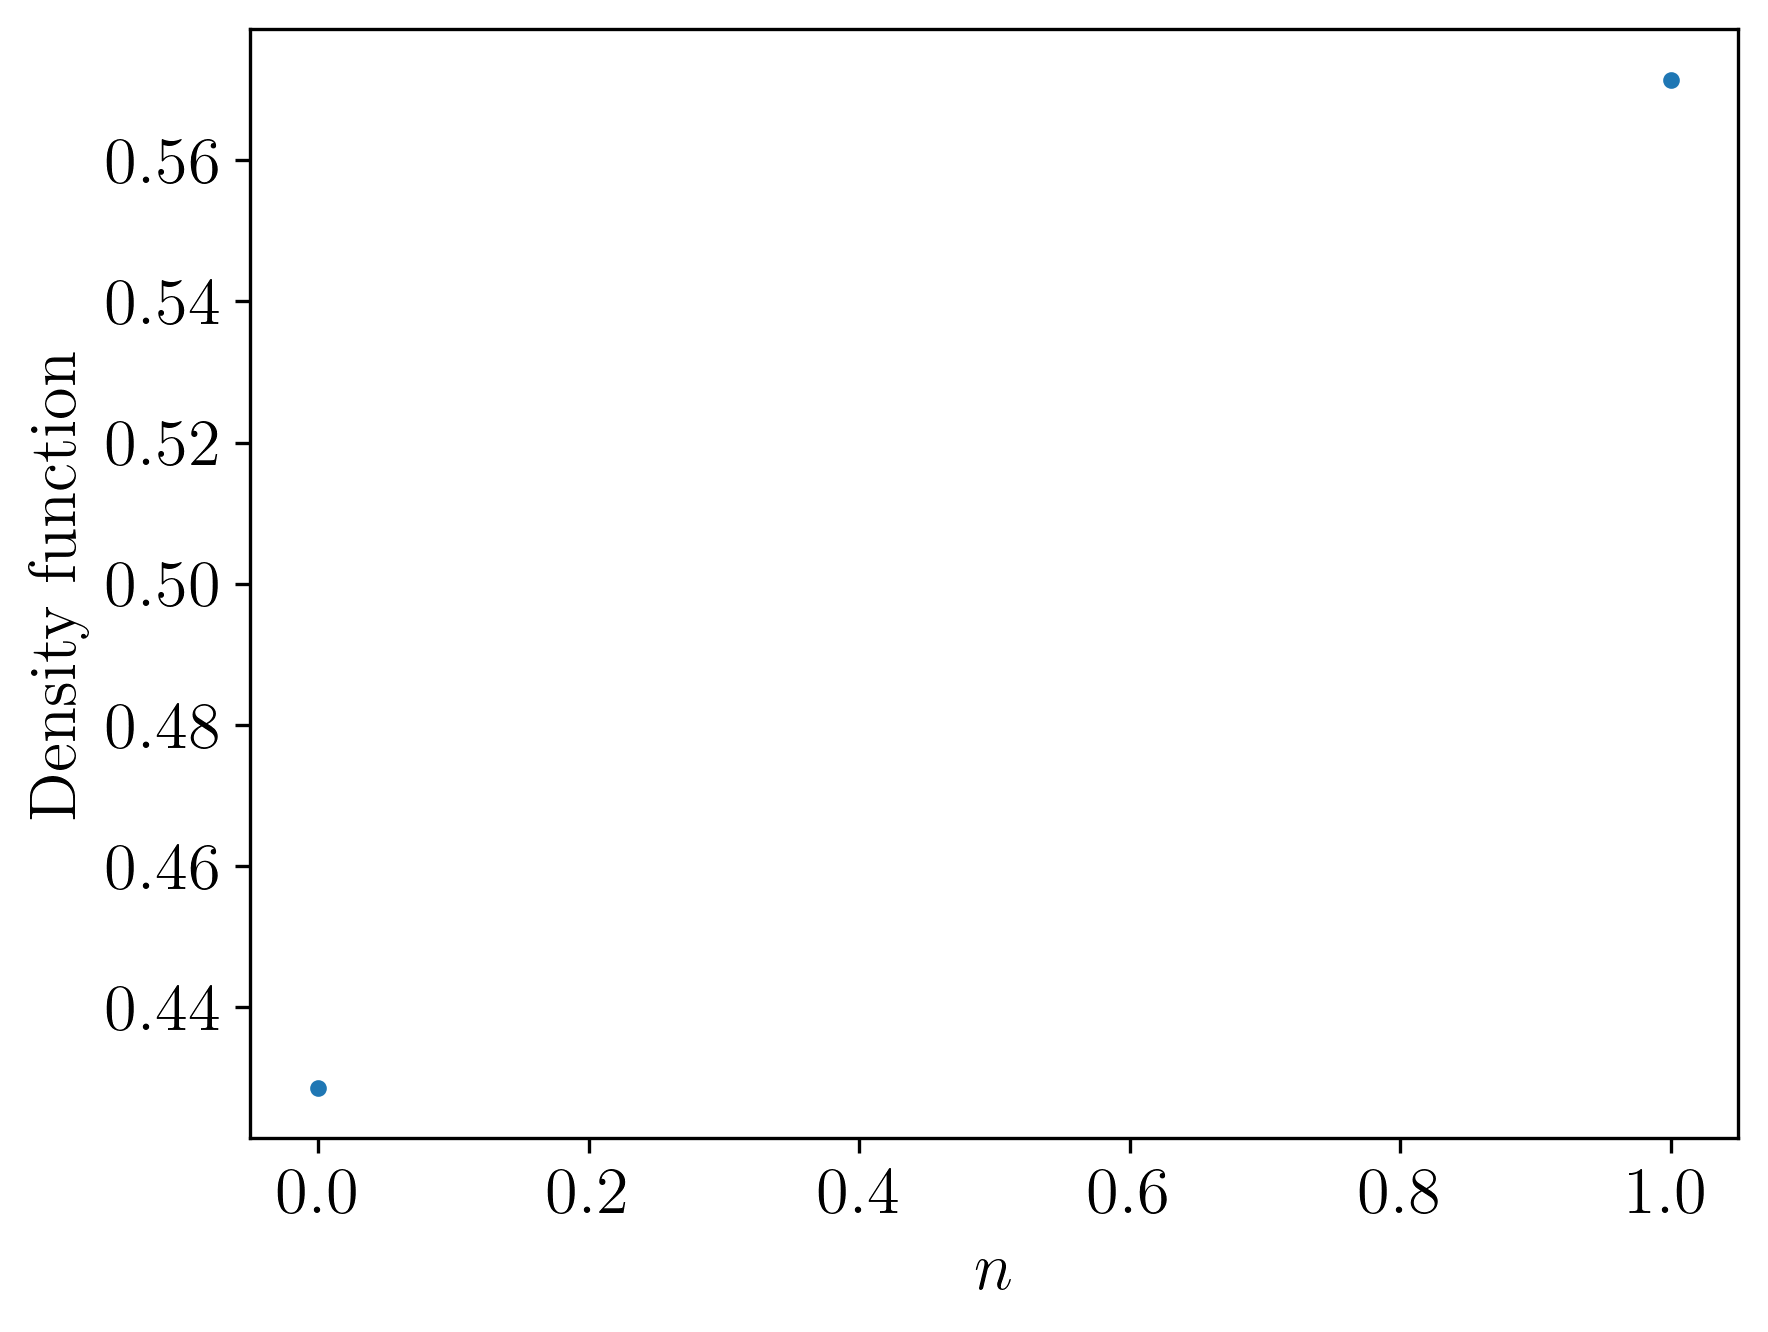
\includegraphics[width=0.5\linewidth]{./Section/Grundlegende Begriffe/Dichte Bernoulli.png}
\caption{Dichte einer $\Ber(4/7)$-Verteilung}
\end{figure}
Wir können diesen Plot auch modifizieren. Mittels
\begin{lstlisting}[numbers=left, numberstyle=\tiny\color{codegray}, firstnumber=6]
fig, ax = rv.plot_density(show=False)
ax.spines['top'].set_visible(False)
ax.spines['right'].set_visible(False)
ax.spines['bottom'].set_position('zero')
ax.spines['left'].set_position('zero')
ax.set_ylim(0)
ax.set_xticks([0, 1])
ax.set_yticks([3/7, 4/7], [r'$\frac{3}{7}$', r'$\frac{4}{7}$'])
plt.savefig('Dichte Bernoulli 2.png', dpi=300)
\end{lstlisting}

\newpage

erhalten wir
\begin{figure}[H]
\centering
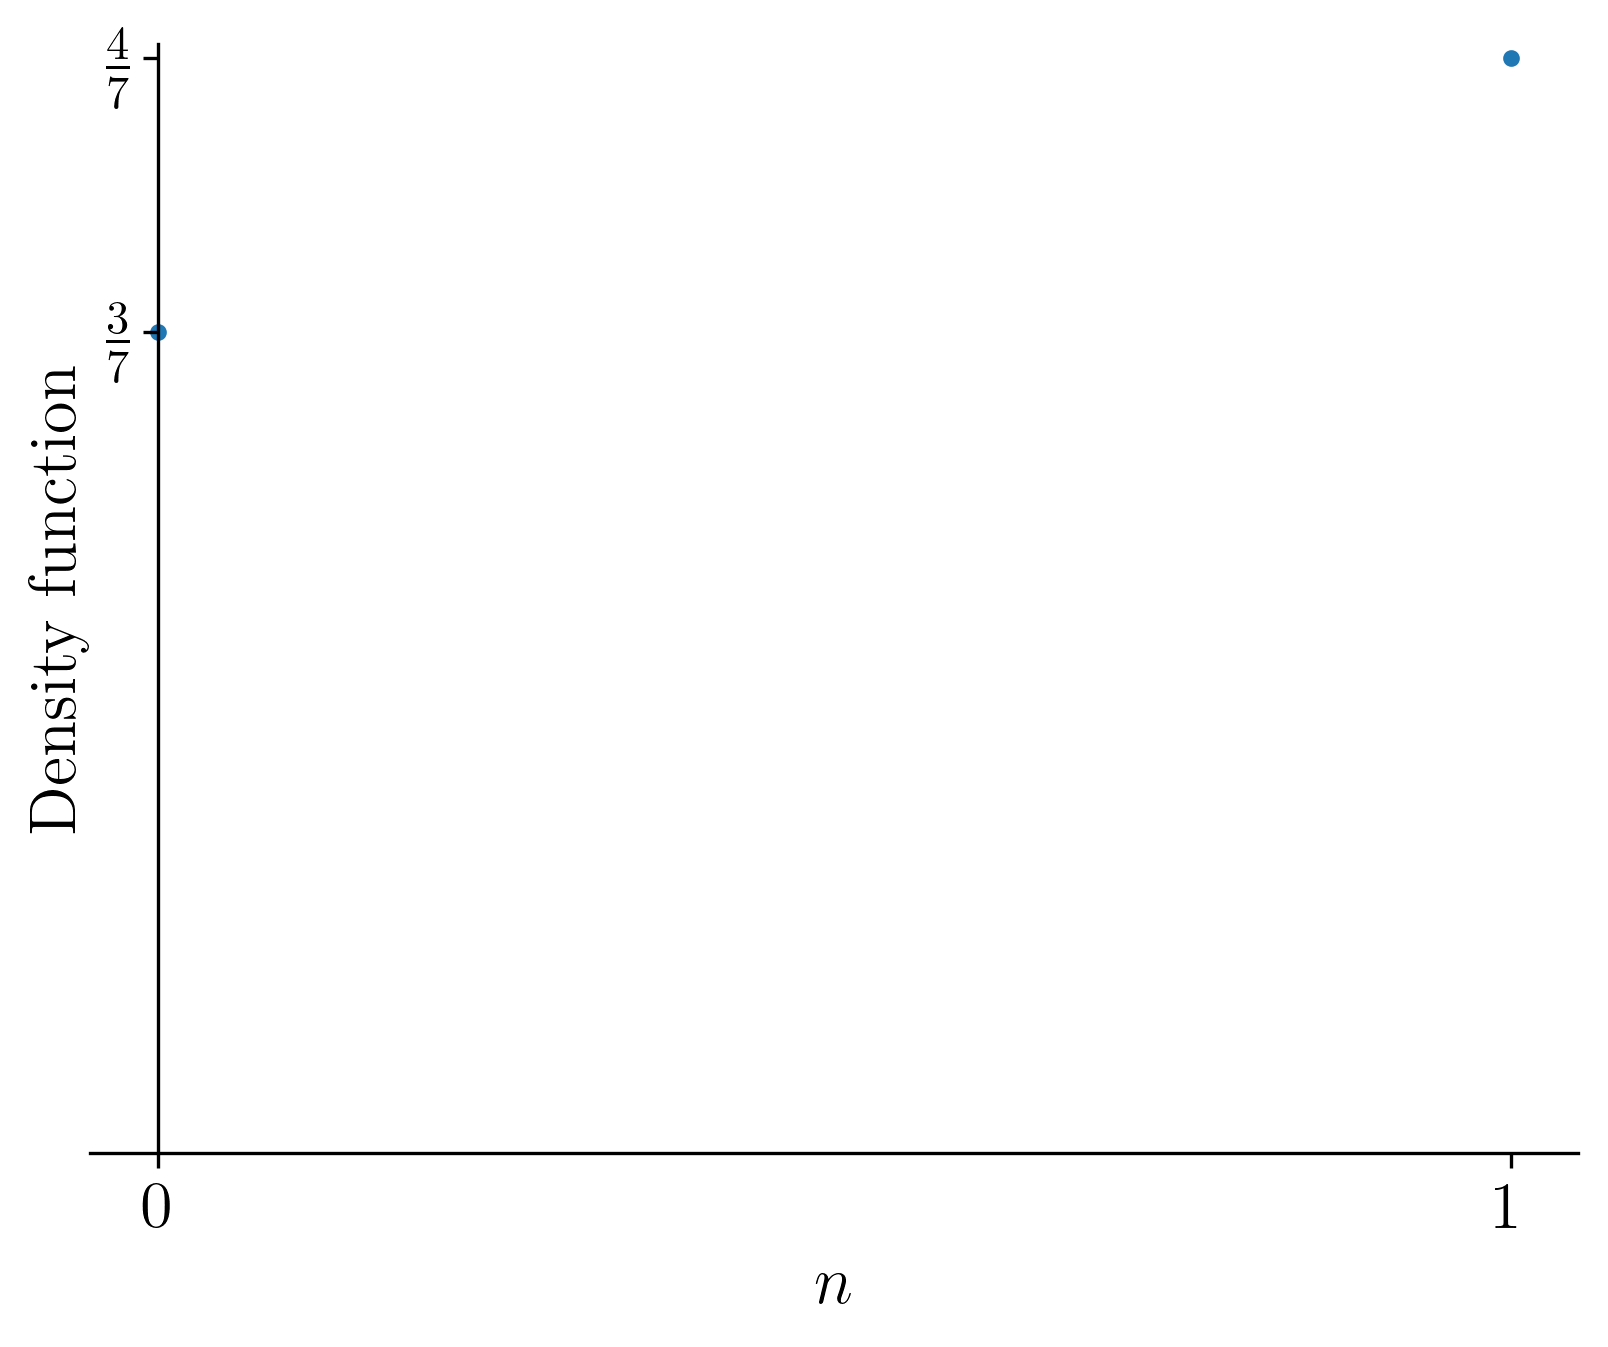
\includegraphics[width=0.5\linewidth]{./Section/Grundlegende Begriffe/Dichte Bernoulli 2.png}
\caption{Dichte einer $\Ber(4/7)$-Verteilung}
\end{figure}

\item Sei $X \sim \Bin(8, 2/3)$. Wir verwenden
\begin{lstlisting}[numbers=left, numberstyle=\tiny\color{codegray}]
k = sym.symbols('k', integer=True, nonnegative=True)
n = sym.Integer(8)
p = sym.Rational(2, 3)
density = sym.binomial(n, k) * p**k * (1 - p)**(n - k)
rv = RandomVariableDiscrete(density, k)
rv.plot_density()
\end{lstlisting}
und erhalten
\begin{figure}[H]
\centering
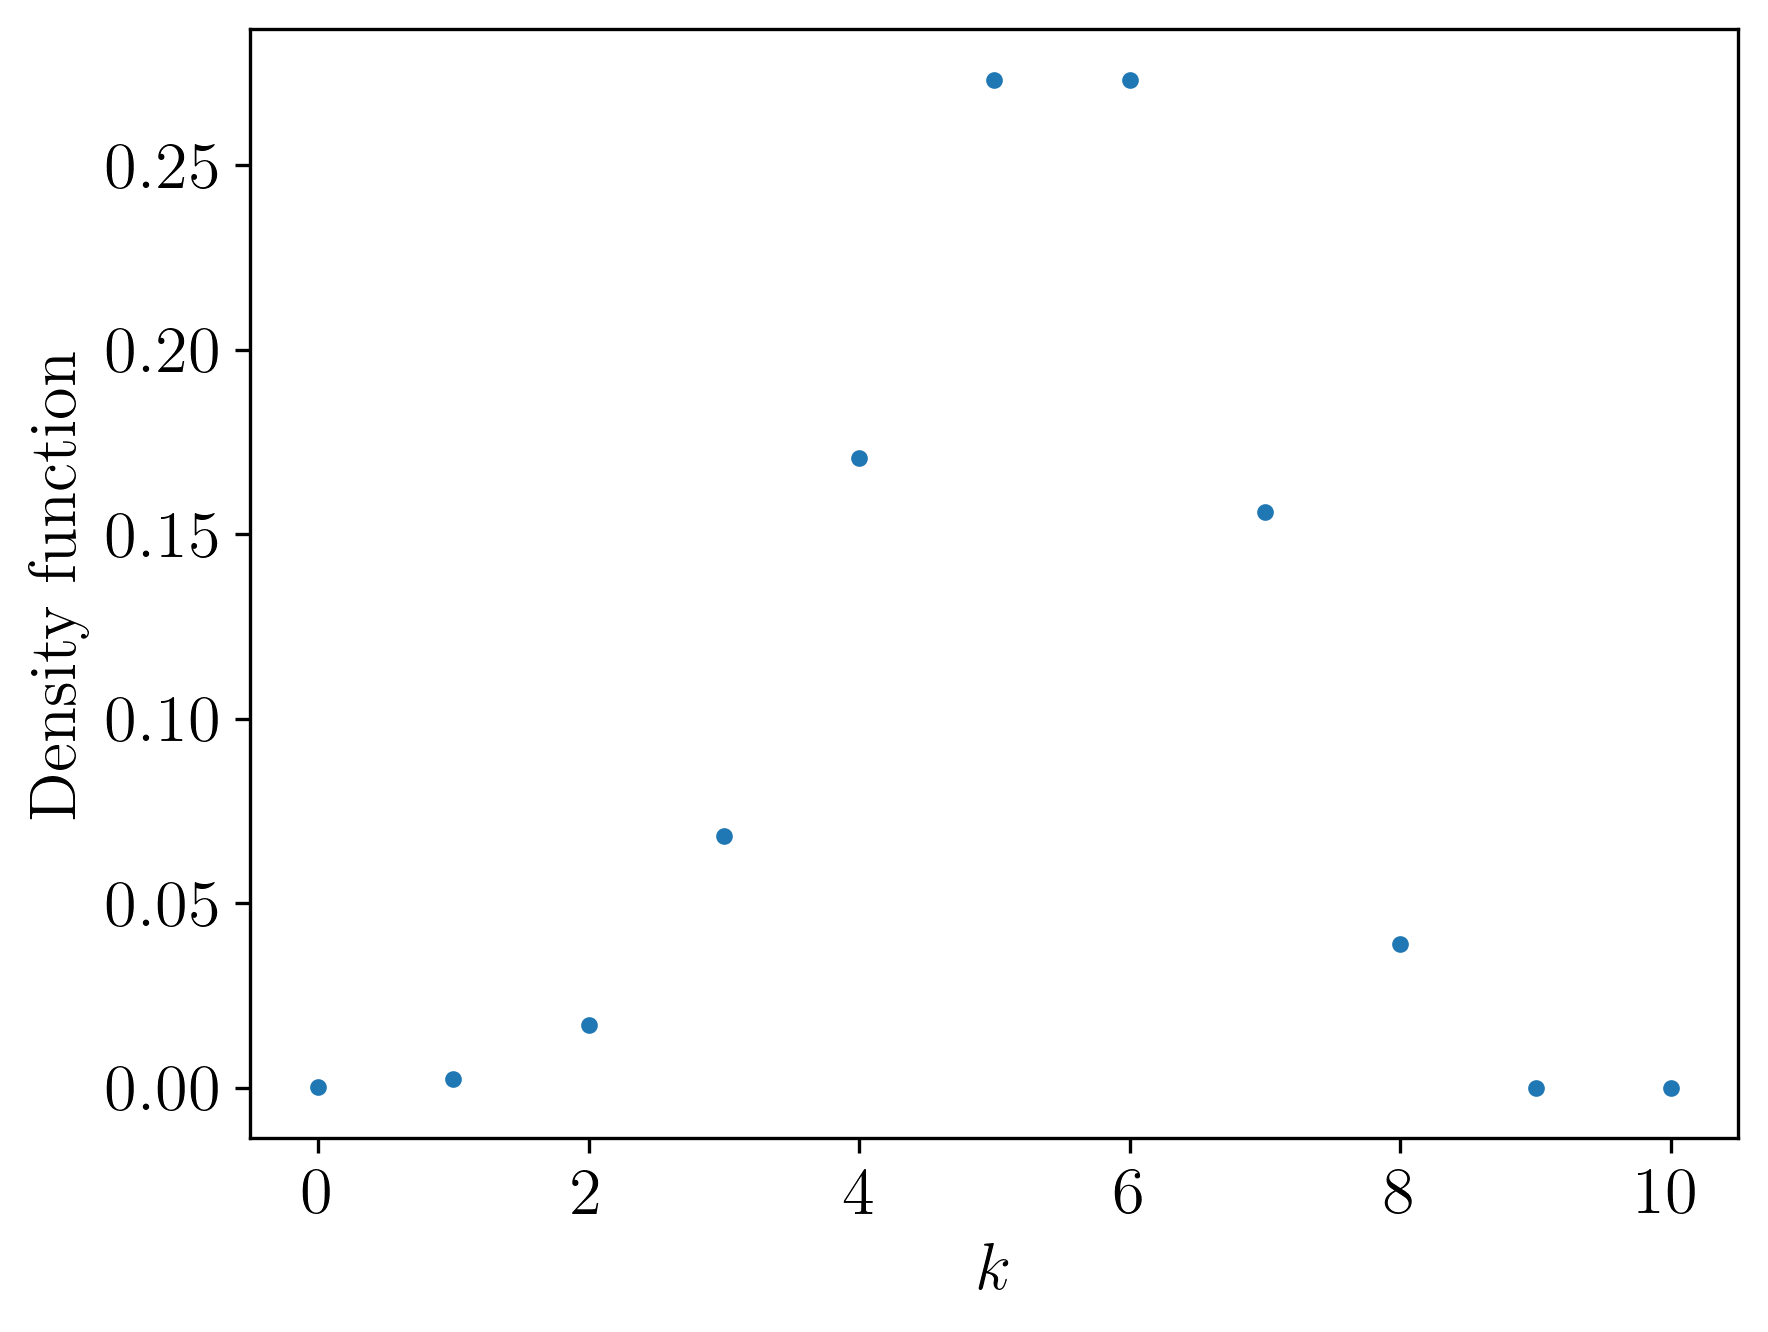
\includegraphics[width=0.5\linewidth]{./Section/Grundlegende Begriffe/Dichte Binomial.png}
\caption{Dichte einer $\Bin(8, 2/3)$-Verteilung}
\end{figure}
Dieser Plot ließe sich auch entsprechend verändern, worauf wir an dieser Stelle aber verzichten wollen.

\item Sei $X \sim \Nor(0, 1)$. Wir verwenden
\begin{lstlisting}[numbers=left, numberstyle=\tiny\color{codegray}]
mu = sym.Integer(0)
sigma = sym.Integer(1)
x = sym.symbols('x', real=True)
density = 1 / (sigma * sym.sqrt(2 * sym.pi)) * sym.exp(- (x - mu)**2 / (2 * sigma**2))
rv = RandomVariableContinuous(density, x)
rv.plot_density()
\end{lstlisting}
und erhalten
\begin{figure}[H]
\centering
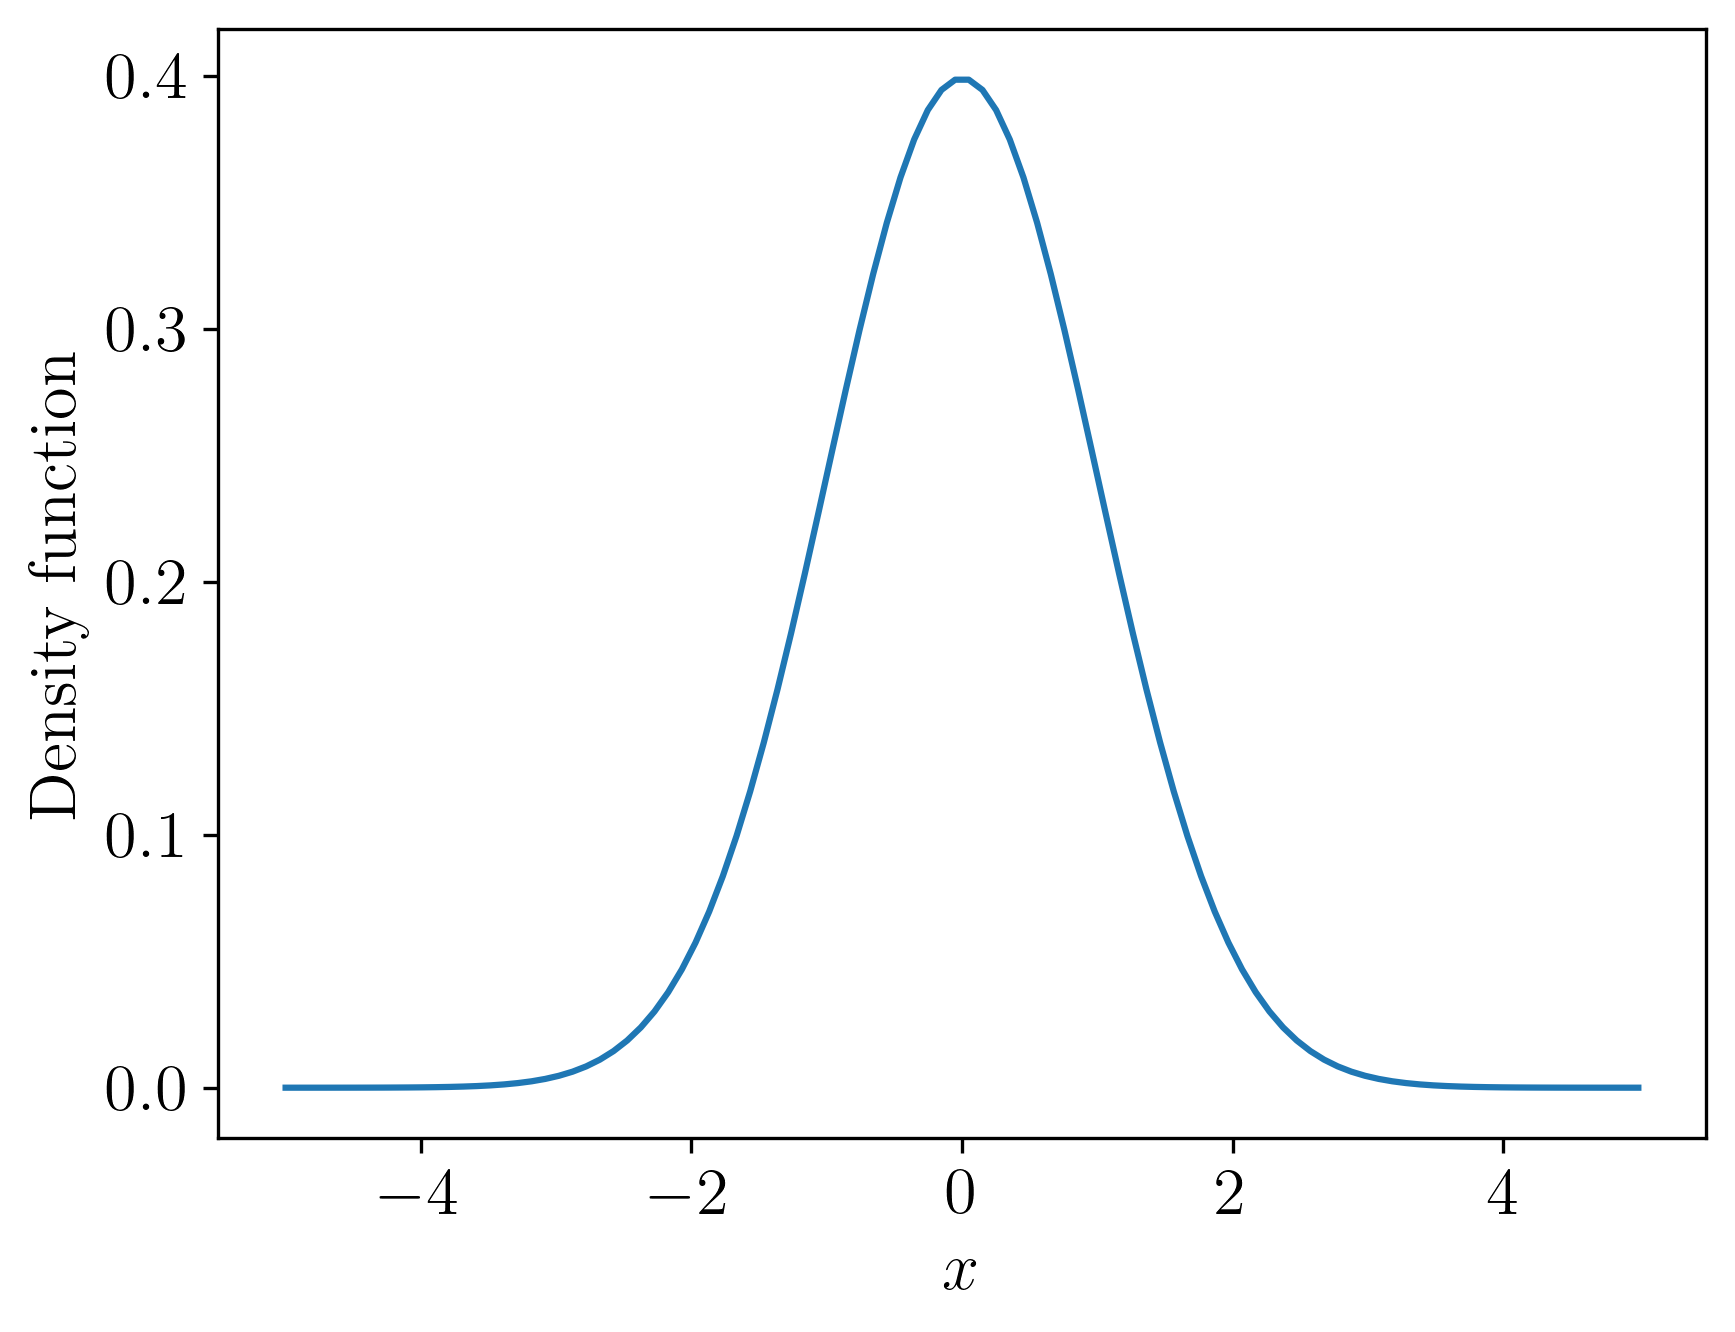
\includegraphics[width=0.5\linewidth]{./Section/Grundlegende Begriffe/Dichte Normal.png}
\caption{Dichte einer $\Nor(0, 1)$-Verteilung}
\end{figure}

\item Sei $X \sim \Exp(3)$. Diesen Plot wollen wir gleich etwas bearbeiten.
\begin{lstlisting}[numbers=left, numberstyle=\tiny\color{codegray}]
lamda = sym.Integer(3)
x = sym.symbols('x', real=True)
density = lamda * sym.exp(- lamda * x)
rv = RandomVariableContinuous(density, x, [sym.Integer(0), sym.oo])
fig, ax = rv.plot_density(numpoints=1000, show=False)
ax.spines['top'].set_visible(False)
ax.spines['right'].set_visible(False)
ax.spines['bottom'].set_position('zero')
ax.spines['left'].set_position('zero')
ax.set_xlim(-1, 4)
ax.set_ylim(0)
plt.show()
\end{lstlisting}
Wir erhalten
\begin{figure}[H]
\centering
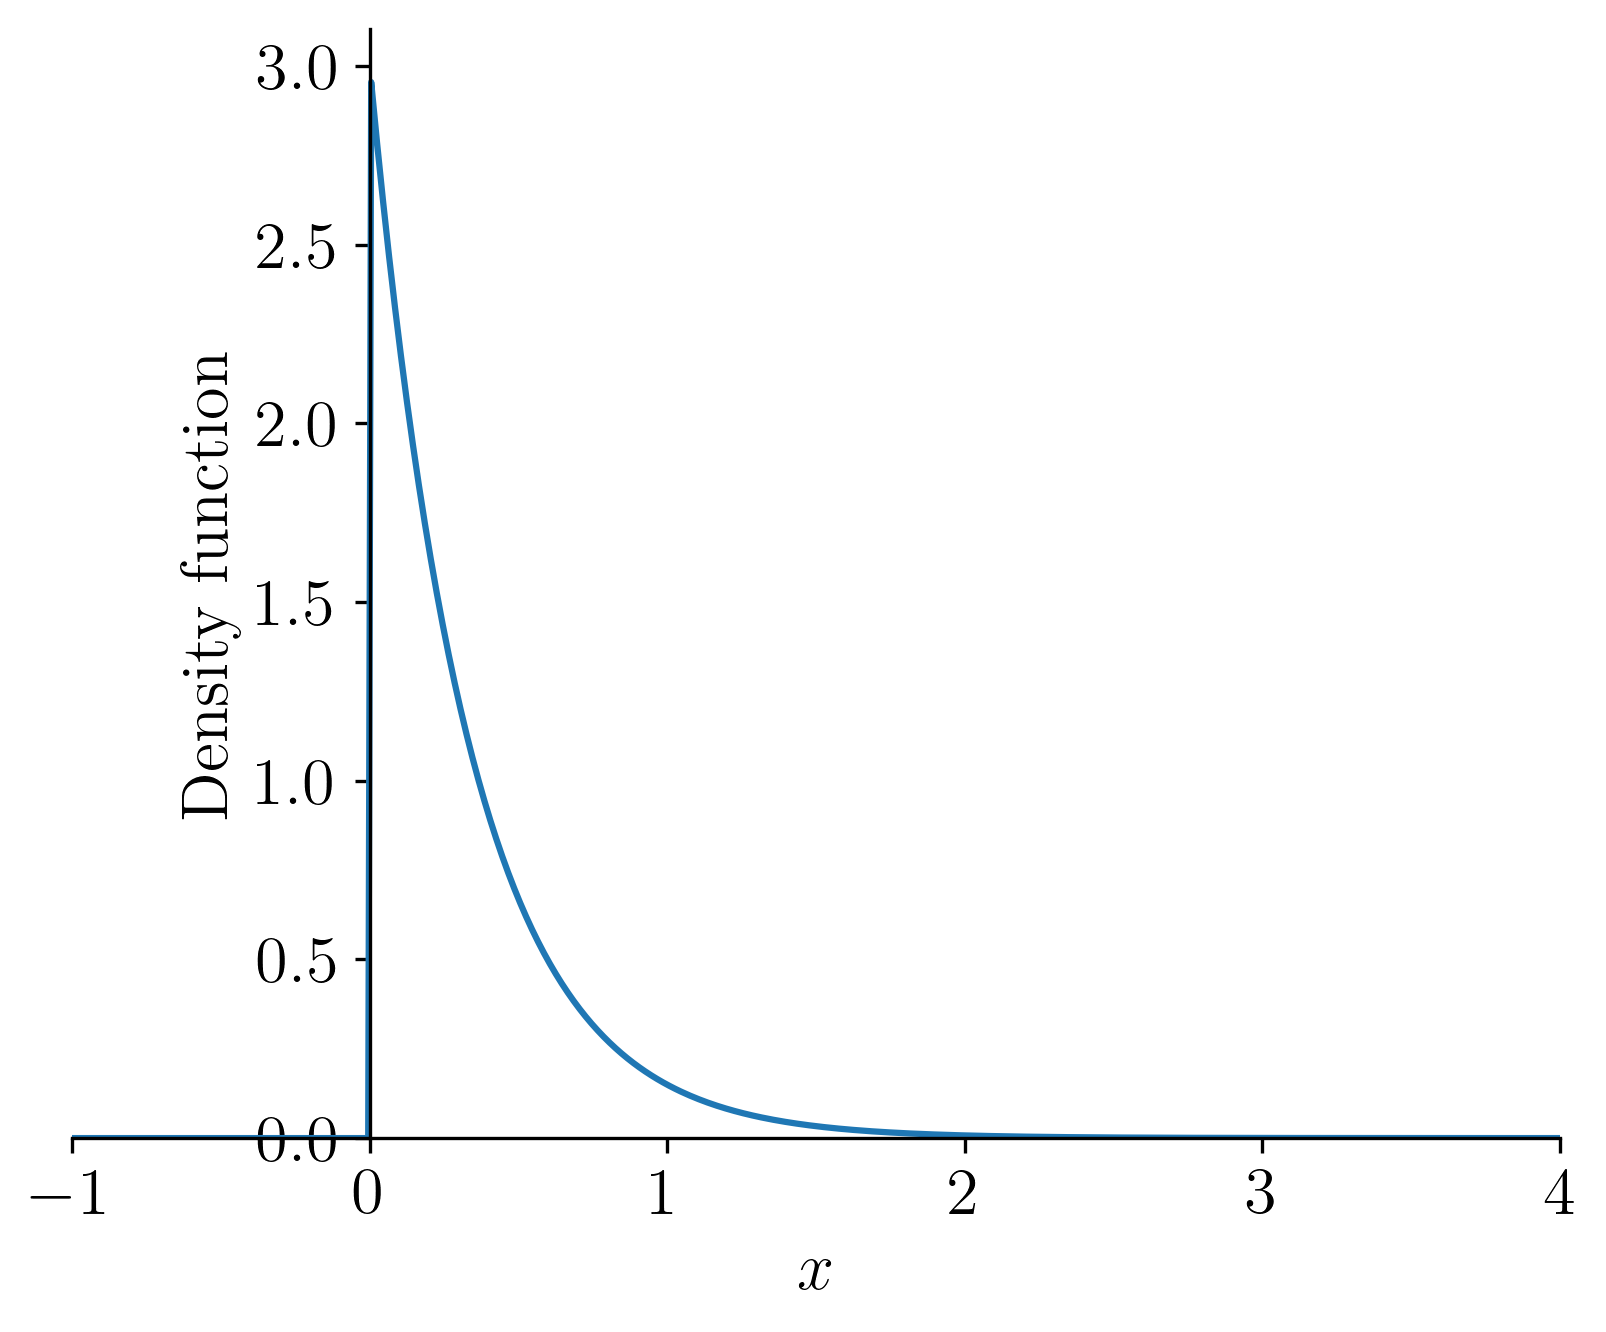
\includegraphics[width=0.5\linewidth]{./Section/Grundlegende Begriffe/Dichte Exponential.png}
\caption{Dichte einer $\Exp(3)$-Verteilung}
\end{figure}
\end{enumerate}
An dieser Stelle sei erwähnt, dass die Senkrechte um die Null mathematisch nicht schön ist. Die Dichte macht an dieser Stelle einen Sprung und diese Unterscheidung wäre in matplotlib theoretisch möglich, hätte aber zu einer unnötigen Spaghettifizierung des Codes geführt.
\end{Beispiel}

\newpage

Wir werden nun einen Satz betrachten und beweisen, mit dem wir Funktionen bezüglich des Bildmaßes integrieren können.

\begin{Satz}{(Maß und Bildmaß)}
\hypertarget{Satz:Maß_und_Bildmaß}{}Sei $(\Omega, \mathscr{A}, \mathbb{P})$ ein Wahrscheinlichkeitsraum und $X$ eine reelle Zufallsvariable. Weiter sei $f: \mathbb{R} \rightarrow \mathbb{R}$ eine messbare Funktion, so dass $f \circ X: \Omega \rightarrow \mathbb{R}$ $\mathbb{P}$-integrierbar ist. Dann gilt
\[\int f \d \mathbb{P}_X = \int f \circ X \d \mathbb{P}~.\]
\end{Satz}

\begin{Beweis}{}
Wir beweisen diesen Satz mittels algebraischer Induktion. Sei $B \in \mathscr{B}$ und $\indi_B$ die zugehörige Indikatorfunktion. Betrachte zunächst für $\omega \in \Omega$
\[\indi_B \circ X(\omega) = 1 \Leftrightarrow X(\omega) \in B \Leftrightarrow \omega \in X^{-1}(B)~.\]
Also gilt
\[\indi_B \circ X = \indi_{X^{-1}(B)}~.\]
Betrachte nun
\begin{align*}
\int \indi_B \d \mathbb{P}_X &= \int_B \d \mathbb{P}_X\\
&= \mathbb{P}_X(B)\\
&= \mathbb{P}(X^{-1}(B))\\
&= \int_{X^{-1}(B)} \d \mathbb{P}\\
&= \int \indi_{X^{-1}(B)} \d \mathbb{P}\\
&= \int \indi_B \circ X \d \mathbb{P}~.
\end{align*}
Sei nun $f$ eine Linearkombination von Indikatorfunktionen mit $(B_n)_{n \in \mathbb{N}_0} \subset \mathscr{B}$ und $(a_n)_{n \in \mathbb{N}_0} \subset \mathbb{R}$. Dann gilt dank Linearität des Integrals
\begin{align*}
\int \sum_{n \in \mathbb{N}_0} a_n \indi_{B_n} \d \mathbb{P}_X &= \sum_{n \in \mathbb{N}_0} a_n \int \indi_{B_n} \d \mathbb{P}_X~.
\intertext{Da dies nur Indikatorfunktionen sind, gilt nach dem ersten Schritt}
&= \sum_{n \in \mathbb{N}_0} a_n \int \indi_{B_n} \circ X \d \mathbb{P}\\
&= \int \sum_{n \in \mathbb{N}_0} a_n \indi_{B_n} \circ X \d \mathbb{P}~.
\end{align*}
Sei $f$ nun eine positive, messbare Funktion. Dann existiert eine monoton steigende Folge $(f_n)_{n \in \mathbb{N}_0}$ von Linearkombination von Indikatorfunktionen mit $\lim_{n \rightarrow \infty} f_n = f$. Dann gilt
\begin{align*}
\int f \d \mathbb{P}_X &= \int \lim_{n \rightarrow \infty} f_n \d \mathbb{P}_X~.
\intertext{Dank dem Satz von Lebesgue lassen sich Limes und Integration vertauschen und es gilt}
&= \lim_{n \rightarrow \infty} \int f_n \d \mathbb{P}_X~.
\intertext{Da dies Linearkombination von Indikatorfunktionen sind, gilt nach obigem}
&= \lim_{n \rightarrow \infty} \int f_n \circ X \d \mathbb{P}~.
\intertext{Nochmaliges Anwenden des Satzes von Lebesgue liefert}
&= \int \lim_{n \rightarrow \infty} f_n \circ X \d \mathbb{P}\\
&= \int f \circ X \d \mathbb{P}~.
\end{align*}
Sei nun $f$ nur noch eine messbare Funktion. Dann gibt es positive, messbare Funktion $f^+$ und $f^-$ mit $f = f^+ - f^+$ und es gilt
\begin{align*}
\int f \d \mathbb{P}_X &= \int f^+ - f^+ \d \mathbb{P}_X\\
&= \int f^+ \d \mathbb{P}_X - \int f^- \d \mathbb{P}_X~.
\intertext{Da dies positive messbare Funktionen sind, folgt dank obigem}
&= \int f^+ \circ X \d \mathbb{P} - \int f^- \circ X \d \mathbb{P}\\
&= \int f^+ \circ X - f^- \circ X \d \mathbb{P}\\
&= \int (f^+ - f^+) \circ X \d \mathbb{P}\\
&= \int f \circ X \d \mathbb{P}~.
\end{align*}
Die Aussage gilt somit für alle messbaren Funktionen und wir sind fertig.
\end{Beweis}
\vspace*{\baselineskip}

Nun werden wir einen Satz beweisen, der es uns erlaubt Funktionen, die wir bezüglich des Bildmaßes integrieren wollen auf einem einfacheren Wege mithilfe der Dichtefunktion zu integrieren.

\begin{Satz}{(Dichtesatz)}
\hypertarget{Satz:Dichtesatz}{}Sei $(\Omega, \mathscr{A}, \mathbb{P})$ ein Wahrscheinlichkeitsraum und $X$ eine reelle Zufallsvariable mit Lebesgue-Dichte $\varphi$. Weiter sei $f: \mathbb{R} \rightarrow \mathbb{R}$ eine Funktion, sodass $f \cdot \varphi$ $\lambda$-integrierbar ist. Dann gilt
\[\int f \d \mathbb{P}_X = \int f \varphi \d \lambda~.\] 
Eine analoge Aussage gilt für das Zählmaß.
\end{Satz}

\begin{Beweis}{}
Wir beweisen diesen Satz mittels algebraischer Induktion. Sei $B \in \mathscr{B}$ und $\indi_B$ die zugehörige Indikatorfunktion. Betrachte
\begin{align*}
\int \indi_B \d \mathbb{P}_X &= \mathbb{P}_X(B)~.
\intertext{Da $\varphi$ eine $\lambda$-Dichte des Maßes $\mathbb{P}_X$ ist, folgt direkt aus der \hyperlink{Def:Dichtefunktion}{\blue{Definition der Dichtefunktion}}}
&= \int \indi_B \varphi \d \lambda~.
\end{align*}
Sei nun $f$ eine Linearkombination von Indikatorfunktionen mit $(B_n)_{n \in \mathbb{N}_0} \subset \mathscr{B}$ und $(a_n)_{n \in \mathbb{N}_0} \subset \mathbb{R}$. Dann gilt dank Linearität des Integrals
\begin{align*}
\int \sum_{n \in \mathbb{N}_0} a_n \indi_{B_n} \d \mathbb{P}_X &= \sum_{n \in \mathbb{N}_0} a_n \int \indi_{B_n} \d \mathbb{P}_X~.
\intertext{Da dies nur Indikatorfunktionen sind, gilt nach dem ersten Schritt}
&= \sum_{n \in \mathbb{N}_0} a_n \int \indi_{B_n} \varphi \d \lambda\\
&= \int \sum_{n \in \mathbb{N}_0} a_n \indi_{B_n} \varphi \d \lambda\\
&= \int \left( \sum_{n \in \mathbb{N}_0} a_n \indi_{B_n} \right) \varphi \d \lambda~.
\end{align*}
Sei $f$ nun eine positive, messbare Funktion. Dann existiert eine monoton steigende Folge $(f_n)_{n \in \mathbb{N}_0}$ von Linearkombinationen von Indikatorfunktionen mit $\lim_{n \rightarrow \infty} f_n = f$. Dann gilt
\begin{align*}
\int f \d \mathbb{P}_x &= \int \lim_{n \rightarrow \infty} f_n \d \mathbb{P}_X~.
\intertext{Dank dem Satz von Lebesgue lassen sich Limes und Integration vertauschen und es gilt}
&= \lim_{n \rightarrow \infty} \int f_n \d \mathbb{P}_X~.
\intertext{Da dies Linearkombinationen von Indikatorfunktionen sind, gilt nach obigem}
&= \lim_{n \rightarrow \infty} \int f_n \varphi \d \lambda~.
\intertext{Nochmaliges Anwenden des Satzes von Lebesgue liefert}
&= \int \lim_{n \rightarrow \infty} f_n \varphi \d \lambda\\
&= \int f \varphi \d \lambda~.
\end{align*}
Sei nun $f$ nur noch eine messbare Funktion. Dann gibt es positive, messbare Funktion $f^+$ und $f^-$ mit $f = f^+ - f^+$ und es gilt
\begin{align*}
\int f \d \mathbb{P}_X &= \int f^+ - f^- \d \mathbb{P}_X\\
&= \int f^+ \d \mathbb{P}_X - \int f^- \d \mathbb{P}_X~.
\intertext{Da dies positive messbare Funktionen sind, folgt dank obigem}
&= \int f^+ \varphi \d \lambda - \int f^- \varphi \d \lambda\\
&= \int f^+ \varphi - f^- \varphi \d \lambda\\
&= \int \left( f^+ - f^- \right) \varphi \d \lambda\\
&= \int f \varphi \d \lambda~.
\end{align*}
Die Aussage gilt somit für alle messbaren Funktionen und wir sind fertig.
\end{Beweis}
\vspace*{\baselineskip}

\newpage

Die Kombination dieser beiden Sätze liefert das folgende Korollar. Dies liefert uns eine einfach Möglichkeit Maßintegrale mit bekannten Werkzeugen zu Riemann- beziehungsweise Lebesgue-Integralen und Reihen zu berechnen.

\begin{Korollar}{(Dichtekorollar)}
\hypertarget{Kor:Dichtekorollar}{}Sei $(\Omega, \mathscr{A}, \mathbb{P})$ ein Wahrscheinlichkeitsraum und $X$ eine reelle Zufallsvariable mit Lebesgue-Dichte $\varphi$. Weiter sei $f: \mathbb{R} \rightarrow \mathbb{R}$ eine messbare Funktion, so dass $f \circ X: \Omega \rightarrow \mathbb{R}$ $\mathbb{P}$-integrierbar und $f \cdot \varphi$ $\lambda$-integrierbar ist. Dann gilt
\[\int f \circ X \d \mathbb{P} = \int f \varphi \d \lambda~.\]
Eine analoge Aussage gilt für das Zählmaß.
\end{Korollar}

\begin{Beweis}{}
Wir verbinden die Aussagen der vorangegangenen Sätze. Betrachte mit dem \hyperlink{Satz:Maß_und_Bildmaß}{\blue{Satz von Maß und Bildmaß}}
\begin{align*}
\int f \circ X \d \mathbb{P} &= \int f \d \mathbb{P}_X\\
&= \int f \varphi \d \lambda~,
\end{align*}
dank dem gerade bewiesenen \hyperlink{Satz:Dichtesatz}{\blue{Dichtesatz}}.
\end{Beweis}
%\vspace*{\baselineskip}

\begin{Bemerkung}{(Dichtekorollar Summenform)}
Wir können das obige \hyperlink{Kor:Dichtekorollar}{\blue{Dichtkorollar}} in die Form für diskrete Zufallsvariablen schreiben. Sei $(\Omega, \mathscr{A}, \mathbb{P})$ ein Wahrscheinlichkeitsraum und $X$ eine diskrete Zufallsvariable mit Zähldichte $\varphi$. Dann gilt für $f : \mathbb{N}_0 \rightarrow \mathbb{R}$
\begin{align*}
\int f \circ X \d \mathbb{P} &= \int f \varphi \d \#\\
&= \sum_{n \in \mathbb{N}_0} f(n) \varphi(n)~.
\end{align*}
Analog gilt dies auch für finite Zufallsvariablen.\\

Sei $X$ nun eine stetige Zufallsvariable mit Dichte $\varphi$. Ist $f \varphi$ für stetige Zufallsvariablen sogar Riemann-integrierbar, so können wir die Integrale wie gewohnt mit dem Hauptsatz berechnen. Diese Voraussetzung nehmen wir im Folgenden häufig implizit an.
\end{Bemerkung}

Wollen wir also die Funktion einer Zufallsvariable bezüglich des Wahrscheinlichkeitsmaßes $\mathbb{P}$ berechnen, so genügt es entsprechende Lebesgue-Integral oder die Summe zu berechnen, falls diese existiert. Wir können nun eine Methode definieren, die genau dieses Korollar anwendet.

\begin{Code}{(\lstinline|integrate_random_variable|)}
\hypertarget{Code:Integrate}{}Ziel dieser Methode ist es Integrale von $f(X)$ zu bestimmen. Sei  $X$ eine reelle Zufallsvariable mit Dichte $\varphi$ und $f$ eine Funktion, die wir mit \lstinline|expr| bezeichnen. Da sich das Zähl- und Lebesgue-Maß grundlegend in ihrer Berechnung unterscheiden, ist diese Methode für jeden Typ von Zufallsvariable separat definiert.
\begin{enumerate}[label=(\roman*)]
\item Für finite Zufallsvariablen gilt
\begin{lstlisting}
def integrate_random_variable(self, expr, lower=-sym.oo, upper=sym.oo):
    integral = sym.Integer(0)
    for key in self.density.keys():
        if key >= lower and key <= upper:
            integral += expr.subs(self.variable, key) * self.density[key]
    integral = sym.simplify(integral)
    return integral
\end{lstlisting}

\newpage

Wir lassen hier untere und obere Grenzen für die Summation zu, welche standardmäßig $- \infty$ und $\infty$ sind. Da die Dichte einer finiten Zufallsvariable aus einem Dictionary besteht, können wir über deren Schlüssel iterieren. Ist der Schlüssel innerhalb des Integrationsintervalls, ersetzen wir mithilfe der \lstinline|subs|-Methode in jeder Iteration die Variable der Funktion durch den entsprechenden Schlüssel und multiplizieren dies mit der Wahrscheinlichkeit diesen Wert zu erhalten, was \lstinline|self.density[key]| entspricht. Zuletzt lassen wir SymPy diesen Ausdruck vereinfachen und anschließend ausgeben.

\item Für diskrete Zufallsvariablen gilt
\begin{lstlisting}
def integrate_random_variable(self, expr, lower=sym.Integer(0), upper=sym.oo):
    lower = sym.Max(lower, self.supp[0])
    upper = sym.Min(upper, self.supp[1])
    integral = sym.summation(expr * self.density, (self.variable, lower, upper)).doit()
    integral = RandomVariable.clean_piecewise(integral)
    integral = sym.simplify(integral)
    return integral
\end{lstlisting}
Wir lassen hier untere und obere Grenzen für die Summation zu, welche standardmäßig $0$ und $\infty$ sind. Diese Summationsgrenzen werden dann noch mit den Grenzen für die Werte der Zufallsvariable verarbeitet. Mithilfe von SymPy bilden wir die Summe aus Funktion und Dichte  und summieren von der unteren bis zur oberen Grenze. Als nächstes wird aus der Hauptklasse die \lstinline|clean_piecewise|-Funktion aufgerufen. Diese überprüft einen Ausdruck, ob dieser zur SymPy \lstinline|Piecewise|-Klasse gehört. Dies ist das SymPy Objekt für stückweise definiert Funktionen. Ist der Ausdruck aus dieser Klasse, so nimmt die Funktion immer den ersten Zweig dieser Funktion, da dieser meist das gesuchte Ergebnis ist und gibt eine Warnung in der Konsole aus. Sollte man nicht wollen, dass stückweise Funktionen gekürzt werden, so kann man die \lstinline|no_chopping|-Funktion aufrufen. Es ist zu beachten, dass dann die meisten Funktionen nicht mehr funktionieren, da SymPy mit stückweisen Funktionen nicht richtig weiterrechnen kann. Zum Schluss wird wieder versucht das Ergebnis zu vereinfachen.

\item Für stetige Zufallsvariablen gilt
\begin{lstlisting}
def integrate_random_variable(self, expr, lower=-sym.oo, upper=sym.oo):
    lower = sym.Max(lower, self.supp[0])
    upper = sym.Min(upper, self.supp[1])
    integral = sym.integrate(expr * self.density, (self.variable, lower, upper)).doit()
    integral = RandomVariable.clean_piecewise(integral)
    integral = sym.simplify(integral)
    return integral
\end{lstlisting}
Wir lassen auch hier obere und untere Grenzen zu, welche standardmäßig auf $\infty$ und $- \infty$ gesetzt werden. Da wir für die Dichten von stetigen Zufallsvariablen die Indikatorfunktionen weggelassen haben, müssen wir diese in einem ersten Schritt mit dem Träger der Dichte vergleichen. Anschließend integrieren wir mit SymPy das Produkt aus Funktion und Dichte von der unteren zur oberen Grenze. Nach der Entfernung von stückweisen Funktionen wird dies wieder vereinfacht und ausgegeben.
\end{enumerate}

Der besonders elegante Teil besteht darin, dass wir in der Aufforderung für die Berechnung quasi die maßtheoretische Integration einer Zufallsvariable verwenden können, da der Code das Dichtekorollar automatisch anwendet und die Dichtefunktion dazu multipliziert.
\end{Code}

\newpage

Wir können nun versuchen mit der obigen Methode eine Funktion einer Zufallsvariable zu integrieren.

\begin{Beispiel}{(Funktionen von Zufallsvariablen)}
\begin{enumerate}[label=(\roman*)]
\item Sei $X$ eine finite Zufallsvariable mit
\begin{align*}
\mathbb{P}(X = 1) &= p\\
\mathbb{P}(X = 2) &= q\\
\mathbb{P}(X = 3) &= 1 - p - q\\
\end{align*}
mit $p, q \in (0, 1)$. Wir berechnen nun mit $E = \{ 1, 2, 3 \}$
\begin{align*}
\int X^2 + 2 X \d \mathbb{P} &= \sum_{n \in E} (n^2 + 2 n) \mathbb{P}(X = n)\\
&= (1^2 + 2 \cdot 1) \mathbb{P}(X = 1) + (2^2 + 2 \cdot 2) \mathbb{P}(X = 2) + (3^2 + 2 \cdot 3) \mathbb{P}(X = 3)\\
&= (1 + 2) p + (4 + 4) q + (9 + 6) (1 - p - q)\\
&= 3 p + 8 q + 15 - 15 p - 15 q\\
&= 15 - 12 p - 7 q
\end{align*}
Dies können wir nun folgendermaßen mit der oben definierten Funktion berechnen lassen.
\begin{lstlisting}[numbers=left, numberstyle=\tiny\color{codegray}]
n = sym.Symbol('n', integer=True, positive=True)
p, q = sym.symbols('p, q', real=True, positive=True)
density = {1: p, 2: q, 3: 1 - p - q}
rv = RandomVariableFinite(density, n)
polynom = rv.integrate_random_variable(n**2 + 2 * n)
\end{lstlisting}
Als Ergebnis erhalten wir \lstinline|-12*p - 7*q + 15|.

\item Sei $X \sim \Exp(\lambda)$ mit $\lambda > 0$ exponentialverteilt. Betrachte nun mit dem \hyperlink{Kor:Dichtekorollar}{\blue{Dichtekorollar}}
\begin{align*}
\int \sin(X) \d \mathbb{P} &= \int_{-\infty}^\infty \sin(x) \lambda \exp(- \lambda x) \indi_{[0, \infty)}(x) \d x\\
&= \lambda \int_0^\infty \sin(x) \exp(- \lambda x) \d x~.
\end{align*}
Weiter betrachten wir das Integral
\begin{align*}
\alpha &= \int_0^\infty \sin(x) \exp(- \lambda x) \d x
\intertext{Mit partieller Integration erhalten wir}
&= \left[ \frac{1}{\lambda} \sin(x) \exp(- \lambda x) \right]_0^\infty + \frac{1}{\lambda} \int_0^\infty \cos(x) \exp(- \lambda x) \d x\\
&= \left[ 0 - 0 \right] + \frac{1}{\lambda} \int_0^\infty \cos(x) \exp(- \lambda x) \d x\\
&= \frac{1}{\lambda} \int_0^\infty \cos(x) \exp(- \lambda x) \d x~.
\displaybreak
\intertext{Nochmal partielle Integration liefert}
&= \left[ - \frac{1}{\lambda^2} \cos \exp(- \lambda x) \right]_0^\infty - \frac{1}{\lambda^2} \int_0^\infty \sin(x) \exp(- \lambda x) \d x\\
&= \left[ - 0 + \frac{1}{\lambda^2} \right] - \frac{1}{\lambda^2} \int_0^\infty \sin(x) \exp(- \lambda x) \d x\\
&= \frac{1}{\lambda^2} - \frac{1}{\lambda^2} \alpha~.
\end{align*}
Zusammengefasst ist also
\begin{align*}
\alpha &= \frac{1}{\lambda^2} - \frac{1}{\lambda^2} \alpha~.
\intertext{Umformen liefert}
(\lambda^2 + 1) \alpha &= 1\\
\alpha &= \frac{1}{\lambda^2 + 1}~.
\end{align*}
Damit ist dann insgesamt
\[\int \sin(X) \d \mathbb{P} = \frac{\lambda}{\lambda^2 + 1}~.\]
Dies können wir folgendermaßen berechnen lassen
\begin{lstlisting}[numbers=left, numberstyle=\tiny\color{codegray}]
x = sym.Symbol('x', real=True)
lamda = sym.Symbol('lambda', real=True, positive=True)
density = lamda * sym.exp(- lamda * x)
rv = RandomVariableContinuous(density, x, [sym.Integer(0), sym.oo])
sine = rv.integrate_random_variable(sym.sin(x))
\end{lstlisting}
Wir erhalten analog \lstinline|lambda/(lambda**2 + 1)|.

\item Sei $X \sim \Nor(0, 1)$ standardnormalverteilt. Wir können mit dieser Methode beispielsweise
\[\int \log(X) \d \mathbb{P}\]
berechnen. Es ist zu beachten, dass $\log$ den natürlichen Logarithmus bezeichnet.
\begin{lstlisting}[numbers=left, numberstyle=\tiny\color{codegray}]
x = sym.Symbol('x', real=True)
density = 1 / sym.sqrt(2 * sym.pi) * sym.exp(- x**2 / 2)
rv = RandomVariableContinuous(density, x)
natural_logarithm = rv.integrate_random_variable(sym.log(x))
\end{lstlisting}
Wir erhalten
\begin{align*}
\int \log(X) \d \mathbb{P} &= - \frac{\log{\left(2 \right)}}{2} - \frac{\gamma}{2} + \frac{i \pi}{2}\\
&= \frac{1}{2} \left( - \log(2) - \gamma + i \pi \right)~.
\end{align*}
Dies ist ein sehr interessantes Ergebnis, da hier einige wichtige mathematische Konstanten auftauchen. Die eulersche Zahl $e$ implizit im natürliche Logarithmus von $2$, die Euler–Mascheroni-Konstante $\gamma$, die komplexe Einheit $i$ und die Kreiszahl $\pi$. Dies können wir leider nicht auf elementare Weise nachrechnen.
\end{enumerate}
Wir werden später in vielen Funktionen diese \lstinline|integrate_random_variable|-Methode benötigen.
\end{Beispiel}

\newpage

Mit dieser Integrationsmethode können wir nun die \lstinline|_is_density|-Methode definieren, welche bei der \hyperlink{Code:Initialisierung}{\blue{Initialisierung einer Zufallsvariable}} aufgerufen wird.

\begin{Code}{(\lstinline|_is_density|)}
Mit dieser Methode überprüfen wir, ob die Wahrscheinlichkeit des gesamten Raumes gleich eins ist. Dies ist folgendermaßen implementiert
\begin{lstlisting}
def _is_density(self):
    total = self.integrate_random_variable(sym.Integer(1))
    if not total.equals(sym.Integer(1)):
        print('WARNING: Density not standardized!')
    return total
\end{lstlisting}
Mithilfe der gerade definieren Integrationsmethode wird über die Einsfunktion integriert. Wir bilden also im stetigen Fall
\begin{align*}
\int_\mathbb{R} 1 \varphi(x) \d x &= \int_\mathbb{R} \varphi(x)  \d x\\
&= \mathbb{P}_X(\mathbb{R})~.
\end{align*}
Für ein Wahrscheinlichkeitsmaß war dies nach \hyperlink{Def:Maß}{\blue{Definition}} eins. Streng genommen müssten wir noch nachrechnen, dass die Dichtefunktion überall nicht-negativ ist. Hierfür gibt es leider keine einfache und effiziente Methode, weshalb diese Überprüfung nicht stattfindet. Diese Methode dient allgemein nur dazu, dem Nutzer offensichtliche Fehler bei der Eingabe der Dichte mitzuteilen. Ist die Dichte nicht normiert, so wird eine entsprechende Warnung in der Konsole ausgegeben. Sollte man diese Überprüfung unterdrücken wollen, so muss man bei der Definition der Zufallsvariable zusätzlich \lstinline|force_denisty=True| übergeben, was die gesamte Überprüfung überspringt. Hier wurde bewusst kein Python-Fehler verwendet. Dieser würde das Programm sofort beenden und es gibt leider Zufallsvariablen, deren Dichten SymPy nicht zu eins vereinfachen kann. Sei dazu $X \sim \Log(p)$ mit $p \in (0, 1)$ logarithmischverteilt. Die Dichte ist gegeben durch
\[\varphi(n) = - \frac{p^n}{n} \frac{1}{\log(1 - p)}\]
für alle $n \in \mathbb{N}$. Wir können daraus nun ein \lstinline|RandomVariable|-Objekt machen.
\begin{lstlisting}[numbers=left, numberstyle=\tiny\color{codegray}]
p = sym.Symbol('p', real=True, positive=True)
n = sym.Symbol('n', integer=True, nonnegative=True)
density = - p**n / n * 1 / sym.log(1 - p)
rv = RandomVariableDiscrete(density, n, supp=[sym.Integer(1), sym.oo])
\end{lstlisting}
Wir erhalten nun die Meldung \lstinline|WARNING: Density not standardized!|. Dies liegt vermutlich daran, dass SymPy die Summe nicht zusammenfassen möchte, da wir nicht festlegen können, dass $p < 1$ ist.
\end{Code}

Da uns Dichtefunktionen die Arbeit erleichtern, wollen wir nun allgemein wissen, wann eine solche Funktion existiert. Für diesen zentralen Satz der Maßtheorie benötigen wir zunächst die folgende

\begin{Definition}{(Nullmenge)}
Sei $(\Omega, \mathscr{A}, \mu)$ ein Maßraum und $A \in \mathscr{A}$ eine Menge. Gilt
\[\mu(A) = 0~,\]
so ist $A$ eine \textit{$\mu$-Nullmenge} oder nur \textit{Nullmenge}.
\end{Definition}

\newpage

Nun können wir einige typische Beispiele für Nullmengen betrachten.

\begin{Beispiel}{(Nullmenge)}
\hypertarget{Bsp:Nullmenge}{}
\begin{enumerate}[label=(\roman*)]
\item Betrachten wir $(\Omega, \mathscr{A}, \delta_{\{\omega\}})$ mit einem $\omega \in \Omega$, so ist jede Menge $A \in \mathscr{A}$ mit $\omega \notin A$ eine $\delta_{\{\omega\}}$-Nullmenge.

\item Betrachten wir $(\mathbb{R}, \mathscr{B}, \lambda)$, so ist jede Einpunktmenge eine Nullmenge. Sei dazu $x \in \mathbb{R}$. Dann gilt
\begin{align*}
\lambda(\{x\}) &= \lambda([x, x])\\
&= x - x\\
&= 0~.
\end{align*}

\item Betrachte wieder $(\mathbb{R}, \mathscr{B}, \lambda)$. Dann ist jede abzählbare Menge eine Nullmenge. Sei nun $A = \{ x_n \in \Omega \mid n \in \mathbb{N}_0 \}$. Dann gilt
\begin{align*}
\lambda(A) &= \lambda\left( \bigsqcup_{n \in \mathbb{N}_0} \{x_n\} \right)~.
\intertext{Aufgrund der $\sigma$-Additivität gilt}
&= \sum_{n \in \mathbb{N}_0} \lambda (\{x_n\})~.
\intertext{Nach (ii) sind dies Nullmenge, womit gilt}
&= \sum_{n \in \mathbb{N}_0} 0\\
&= 0~.
\end{align*}
Insbesondere sind $\mathbb{N}$, $\mathbb{Z}$ und $\mathbb{Q}$ Lebesgue-Nullmengen.
\end{enumerate}
\end{Beispiel}

\vspace*{-0.75\baselineskip}

\begin{Definition}{(Absolute Stetigkeit)}
Seien $\mu$ und $\nu$ Maße auf $(\Omega, \mathscr{A})$. Gilt für alle $A \in \mathscr{A}$ mit $\mu(A) = 0$ auch $\nu(A) = 0$, so ist $\nu$ \textit{absolutstetig} bezüglich $\mu$ und wir schreiben $\nu \ll \mu$.
\end{Definition}

Mithilfe dieser Definitionen können wir nun den folgenden Satz formulieren, der uns dabei hilft, verstehen zu können, wann Dichten existieren.

\begin{Satz}{(Radon-Nikodym)}
\hypertarget{Satz:Radon-Nikodym}{}Seien $\mu$ und $\nu$ zwei $\sigma$-endliche Maße auf $(\Omega, \mathscr{A})$. Dann sind die folgenden Aussagen äquivalent.
\begin{enumerate}[label=\textup{(\roman*)}]
\item $\nu$ ist absolutstetig bezüglich $\mu$.
\item $\nu$ hat eine Dichte bezüglich $\mu$.
\end{enumerate}
\end{Satz}

%\vspace*{-0.5\baselineskip}

Dies ist ein zentraler Satz der Maß- und Wahrscheinlichkeitstheorie. Der Satz von Radon-Nikodym ist nicht nur eine Existenz-Aussage sondern er liefert uns auch eine \glqq Bauanleitung\grqq{}, wie wir eine solche Dichte finden können. Darauf wollen wir aber im Folgenden nicht weiter eingehen.

\newpage
Nun können wir einige Beispiele zur Anwendung des Satzes von Radon-Nikodym betrachten.

\begin{Beispiel}{(Anwendungen Radon-Nikodym)}
\begin{enumerate}[label=(\roman*)]
\item Gegeben sei die Zufallsvariable $X$ aus dem \hyperlink{Bsp:Regen}{\blue{Regenbeispiel}}. Die Lebesgue-Dichte ist
\[\varphi(x) = \indi_{[0, 1]}(x)~.\]
Nach dem \hyperlink{Satz:Radon-Nikodym}{\blue{Satz von Radon-Nikodym}} ist das Bildmaß $\mathbb{P}_X$ absolutstetig bezüglich dem Lebesgue-Maß $\lambda$ und alle Lebesgue-Nullmengen sind auch Nullmengen bezüglich dem Bildmaß $\mathbb{P}_X$. Wir können also folgern, dass die Wahrscheinlichkeit, dass der Regentropfen auf einem bestimmten Punkt auftritt, null ist.

\item Gegeben sei ein Dirac-Maß zu $x \in \mathbb{R}$. Nach dem \hyperlink{Bsp:Nullmenge}{\blue{Beispiel zu Nullmengen}} ist $\{x\}$ eine Lebesgue-Nullmenge. Da aber $\delta_{\{x\}}(\{x\}) = 1$ ist, ist $\delta_{\{x\}}$ nicht absolutstetig bezüglich $\lambda$. Aus dem \hyperlink{Satz:Radon-Nikodym}{\blue{Satz von Radon-Nikodym}} folgt, dass das Dirac-Maß keine Lebesgue-Dichte besitzen kann.

\item Sei $X \sim \Ber(p)$ mit $p \in (0, 1)$. Da
\[\mathbb{P}_X(1) = p \neq 0\]
ist, kann $X$ nach dem \hyperlink{Satz:Radon-Nikodym}{\blue{Satz von Radon-Nikodym}} keine Lebesgue-Dichte besitzen. $X$ hat dafür eine Zähldichte.
\end{enumerate}
Es gibt auch Zufallsvariablen, die weder eine Lebesgue- noch eine Zähldichte besitzen.
\end{Beispiel}

Im Folgenden werden wir uns ausschließlich mit Zufallsvariablen beschäftigen, die eine Zähl- oder Lebesgue-Dichte besitzen.

\subsection{Verteilungsfunktionen}

In diesem Abschnitt werden wir uns mit einer wichtigen Funktion beschäftigen, die für jede reelle Zufallsvariable existiert.

\begin{Definition}{(Verteilungsfunktion)}
Sei $X$ eine reelle Zufallsvariable. Durch 
\[F_X: \mathbb{R} \rightarrow [0, 1]: x \mapsto F_X(x) := \mathbb{P}(X \leq x)\]
ist die \textit{Verteilungsfunktion} definiert.
\end{Definition}

Wir werden nun einige Eigenschaften von Verteilungsfunktionen beweisen.

\begin{Satz}{(Eigenschaften Verteilungsfunktion)}
\hypertarget{Satz:EigVertFun}{}Sei $(\Omega, \mathscr{A}, \mathbb{P})$ ein Wahrscheinlichkeitsraum und $X$ eine reelle Zufallsvariable. Die Verteilungsfunktion $F_X$ hat dann die folgenden Eigenschaften.
\begin{enumerate}[label=\textup{(\roman*)}]
\item $F_X$ ist rechtsseitig stetig.
\item $F_X$ ist monoton wachsend.
\item $\lim_{x \rightarrow -\infty} F_X(x) = 0$.
\item $\lim_{x \rightarrow \infty} F_X(x) = 1$.
\end{enumerate}
\end{Satz}

\newpage

\begin{Beweis}{}
Zu (i):\\
Sei $x \in \mathbb{R}$ beliebig und $(x_n)_{n \in \mathbb{N}_0}$ eine monoton fallende Folge mit Grenzwert $x$. Betrachte
\begin{align*}
\lim_{n \rightarrow \infty} F_X(x) &= \lim_{n \rightarrow \infty} \mathbb{P}(X \leq x_n)~.
\intertext{Da $\mathbb{P}$ als Wahrscheinlichkeitsmaß insbesondere stetig von oben ist, kann man den Limes reinziehen und erhält}
&= \mathbb{P}(X \leq x)\\
&= F_X(x)~.
\end{align*}
Somit ist $F_X$ rechtsseitig stetig.\\

Zu (ii):\\
Sei $x_1 \leq x_2$ aus $\mathbb{R}$. Betrachte
\begin{align*}
F_X(x_2) - F_X(x_1) &= \mathbb{P}(X \leq x_2) - \mathbb{P}(X \leq x_1)\\
&= \int_\mathbb{R} \indi_{(-\infty, x_2]} \d \mathbb{P}_X - \int_\mathbb{R} \indi_{(-\infty, x_2]} \d \mathbb{P}_X~.
\intertext{Mit der Linearität des Integrals gilt}
&= \int_\mathbb{R} \indi_{(-\infty, x_2]} - \indi_{(-\infty, x_1]} \d \mathbb{P}_X~.
\intertext{Wir werden gleich sehen, dass folgenden Umformung eine Identität ist}
&= \int_\mathbb{R} \indi_{[x_1, x_2]} \d \mathbb{P}_X\\
&= \mathbb{P}(X \in [x_1, x_2]) \geq 0~,
\end{align*}
dank (M2). Umformen liefert
\[F_X(x_2) \geq F_X(x_1)~.\]
Zum Beweis der oben verwendeten Identität, betrachte die folgende Tabelle:

\begin{center}
\renewcommand{\arraystretch}{1.5}
\begin{tabularx}{\linewidth}{c | c c c c}
& $\indi_{(-\infty, x_1]}(x)$ & $\indi_{(-\infty, x_2]}(x)$ & $\indi_{(-\infty, x_2]}(x) - \indi_{(-\infty, x_1]}(x)$ & $\indi_{[x_1, x_2]}(x)$\\
\hline
$x \in (-\infty, x_1]$ & $1$ & $1$ & $0$ & $0$\\
$x \in (x_1, x_2)$ & $0$ & $1$ & $1$ & $1$\\
$x \in [x_2, \infty)$ & $0$ & $0$ & $0$ & $0$
\end{tabularx}
\end{center}

Da die letzten beiden Spalten immer übereinstimmen gilt für alle $x \in \mathbb{R}$
\[\indi_{(-\infty, x_2]}(x) - \indi_{(-\infty, x_1]}(x) = \indi_{[x_1, x_2]}(x)~.\]

Zu (iii):\\
Betrachte
\begin{align*}
\lim_{x \rightarrow -\infty} F_X(x) &= \lim_{x \rightarrow -\infty} \mathbb{P}(X \leq x)\\
&= \lim_{x \rightarrow -\infty} \int \indi_{(-\infty, x]} \d \mathbb{P}_X~.
\intertext{Mit dem Satz von Lebesgue können wir Integration und Limesbildung vertauschen und es gilt}
&= \int \lim_{x \rightarrow -\infty} \indi_{(-\infty, x]} \d \mathbb{P}_X\\
&= \int \indi_{\emptyset} \d \mathbb{P}_X \\
&= \mathbb{P}_X(\emptyset) = 0~,
\end{align*}
da $\mathbb{P}_X$ als Maß insbesondere nulltreu ist.\\

Zu (iv):\\
Betrachte
\begin{align*}
\lim_{x \rightarrow \infty} F_X(x) &= \lim_{x \rightarrow \infty} \mathbb{P}(X \leq x)\\
&= \lim_{x \rightarrow \infty} \int \indi_{(-\infty, x]} \d \mathbb{P}_X~.
\intertext{Mit dem Satz von Lebesgue können wir Integration und Limesbildung vertauschen und es gilt}
&= \int \lim_{x \rightarrow \infty} \indi_{(-\infty, x]} \d \mathbb{P}_X\\
&= \int \indi_\mathbb{R} \d \mathbb{P}_X \\
&= \mathbb{P}_X(\mathbb{R}) = 1~,
\end{align*}
da $\mathbb{P}_X$ ein Wahrscheinlichkeitsmaß ist.
\end{Beweis}

\vspace*{\baselineskip}

Wir werden nun eine Möglichkeit finden, diese Verteilungsfunktion auf einfache Weise zu berechnen.

\begin{Bemerkung}{(Berechnung der Verteilungsfunktion)}
\hypertarget{Verteilungsfunktion}{} Sei $X$ eine stetige Zufallsvariable mit Dichte $\varphi$. Dann gilt dank dem \hyperlink{Kor:Dichtekorollar}{\blue{Dichtekorollar}}
\begin{align*}
F_X(x) &= \mathbb{P}(X \leq x)\\
&= \int \indi_{\{\omega: X(\omega) \leq x\}}(\omega) \d \mathbb{P}(\omega)\\
&= \int \indi_{X \in (- \infty, x]} \d \mathbb{P}\\
&= \int \indi_{(-\infty, x]} \varphi \d x\\
&= \int_{-\infty}^x \varphi \d x~.
\end{align*}
Wir können also einfach die Einsfunktion bis zum Wert $x$ integrieren. Für diskrete Zufallsvariablen berechnen wir
\[F_X(x) = \sum_{n = 0}^{\lfloor x \rfloor} \varphi(n)~.\]
Es sei an dieser Stelle nochmal erwähnt, dass die Verteilungsfunktion eine Funktion von $\mathbb{R}$ nach $[0, 1]$ ist. Wir können also jeden reellen Wert einsetzen und nicht nur Werte, die $X$ annehmen kann. Deshalb müssen wir hier die Abrundungsfunktion $\lfloor \cdot \rfloor$ verwenden.
\end{Bemerkung}

\newpage

Wir können nun eine Methode schreiben, welche zu einer Zufallsvariable die Verteilungsfunktion berechnet.

\begin{Code}{(\lstinline|distribution_function|)}
Die Berechnung der Verteilungsfunktion ist leider etwas komplizierter. Aufgrund dessen müssen wir hier wieder die verschiedenen Typen unterscheiden.
\begin{enumerate}[label=(\roman*)]
\item Für finite Zufallsvariablen gilt
\begin{lstlisting}
def distribution_function(self):
    sortable = True
    keys = list(self.density.keys())
    for key in keys:
        if isinstance(key, sym.Symbol):
            print('WARNING: Can\'t sort values.')
            sortable = False
            break
    if sortable:
        keys = sorted(keys)
    cumulative_probability = self.density[keys[0]]
    distribution_function = {keys[0]: cumulative_probability}
    keys.pop(0)
    for key in keys:
        cumulative_probability += self.density[key]
        distribution_function.update({key: cumulative_probability})
    return distribution_function
\end{lstlisting}
Im ersten Schritt wird überprüft, ob die Werte der Zufallsvariable, also die Keys des Dictionaries, sortierbar sind. Sind sie nicht sortierbar, so wird die Verteilungsfunktion aufgrund der gegebenen Reihenfolge berechnet. Nun wird die erste kumulierte Wahrscheinlichkeit festgelegt und diese mit dem entsprechenden Wert der Zufallsvariable der Verteilungsfunktion hinzugefügt. Zuletzt wird dieser Wert aus der Liste der Werte entfernt. Im nächsten Schritt wird über alle anderen Werte iteriert. Dazu wird die Wahrscheinlichkeit für den entsprechenden Wert der kumulierte Wahrscheinlichkeit hinzuaddiert und das Dictionary um das entsprechende Paar erweitert. Man erhält am Schluss also ein Dictionary. Die Keys sind die ersten Werte, ab denen die sich im Value befindende kumulierte Wahrscheinlichkeit angenommen wird. Dies sind also jeweils nach links geschlossene halboffene Intervalle. Insbesondere ist auf dem offenen Intervall von $- \infty$ bis zum ersten Wert die kumulierte Wahrscheinlichkeit (implizit) null. 

\item Für diskrete Zufallsvariablen gilt
\begin{lstlisting}
def distribution_function(self, value=None):
    if value == None:
        t = sym.Symbol('t', real=True)
        upper = sym.Min(self.supp[1], sym.floor(t))
        distribution_function = self.integrate_random_variable(sym.Integer(1), upper=upper)
        return distribution_function
    else:
        value = sym.sympify(value)
        upper = sym.Min(self.supp[1], sym.floor(value))
        distribution_function = self.integrate_random_variable(sym.Integer(1), upper=upper)
        distribution_function = float(distribution_function.evalf())
        return distribution_function
\end{lstlisting}
Die Berechnung der Verteilungsfunktion für diskrete Zufallsvariablen läuft über zwei verschiedene Arten ab. Ruft man die Methode ohne weiteres Argument auf, so ergibt sich die obere Grenze über die Abrundungsfunktion $\lfloor t \rfloor$ und das Minimum mit der oberen Schranke für den Wertebereich. Anschließend wird über die Eins summiert bis zu dieser oberen Grenze.

\newpage

Verwendet man als Argument eine Zahl, so wird diese ebenfalls abgerundet und das Minimum mit der oberen Grenze gebildet. Auch hier wird die Summe über die Eins gebildet. Anders als zuvor wird dieser Wert nun evaluiert und in eine Gleitkommazahl umgewandelt. Diese zweite Methode wird später für den \hyperlink{Code:PlotDistr}{\blue{Plot der Verteilungsfunktion}} und die \hyperlink{Sec:Sim}{\blue{Simulation}} wichtig.

\item Für stetige Zufallsvariablen gilt
\begin{lstlisting}
def distribution_function(self):
    t = sym.Symbol('t', real=True)
    distribution_function = self.integrate_random_variable(sym.Integer(1), upper=t)
    return distribution_function
\end{lstlisting}
Diese Berechnung ist viel näher an der Definition der Verteilungsfunktion. Dabei wird die Einsfunktion mithilfe der Integrationsmethode integriert, wobei die obere Grenze die Variable der Verteilungsfunktion ist.
\end{enumerate}
\end{Code}

\vspace*{-\medskipamount}

Wir können nun einige Verteilungsfunktionen berechnen.

\begin{Beispiel}{(Verteilungsfunktionen)}
\hypertarget{Bsp:VertFun}{}Da diskrete Zufallsvariablen Treppenfunktionen als Verteilungsfunktionen haben und sich die Summen nicht weiter zusammenfassen lassen, werden wir nur finite und stetige Beispiele betrachten.
\begin{enumerate}[label=(\roman*)]
\item Sei $X \sim \Ber(p)$ mit $p \in (0, 1)$ Bernoulli-verteilt. Wir finden die folgende Verteilungsfunktion
\[F_X(x) = \begin{cases}
0 &, x \in (- \infty, 0)\\
1 - p &, x \in [0, 1)\\
1 &, x \in [1, \infty)~.
\end{cases}\]
Mittels
\begin{lstlisting}[numbers=left, numberstyle=\tiny\color{codegray}]
n = sym.Symbol('n', integer=True,positive=True)
p = sym.Symbol('p', real=True, positive=True)
density = {1: p, 0: 1 - p}
rv = RandomVariableFinite(density, n)
distribution_function = rv.distribution_function()
\end{lstlisting}
erhalten wir \lstinline|{0: 1 - p, 1: 1}|. Dies entspricht genau dem oben Berechneten.
\item Sei $X \sim \Exp(\lambda)$ mit $\lambda > 0$ exponentialverteilt. Für $x \geq 0$ betrachten wir deshalb
\begin{align*}
F_X(x) &= \mathbb{P}(X \leq x)\\
&= \int_{-\infty}^x \lambda \exp(- \lambda x) \indi_{[0, \infty)}(x) \d x\\
&= \int_0^x \lambda \exp(- \lambda x) \d x\\
&= \left[ - \exp(- \lambda x) \right]_0^x\\
&= - \exp(- \lambda x) + 1~.
\end{align*}
Nach den \hyperlink{Satz:EigVertFun}{\blue{Eigenschaften der Verteilungsfunktion}} ist für $x < 0$ dann $F_X(x) = 0$. Um den oberen Teil der Verteilungsfunkion mit SymPy auszurechnen, verwenden wir
\begin{lstlisting}[numbers=left, numberstyle=\tiny\color{codegray}]
x = sym.Symbol('x', real=True)
lamda = sym.Symbol('lambda', real=True, positive=True)
density = lamda * sym.exp(- lamda * x)
rv = RandomVariableContinuous(density, x, [sym.Integer(0), sym.oo])
distribution_function = rv.distribution_function()
\end{lstlisting}
und erhalten \lstinline|1 - exp(-lambda*t)| wie oben.
\item Sei $X$ auf $[0, 1]$ stetig gleichverteilt. Betrachte zu $x \in [0, 1]$
\begin{align*}
F_X(x) &= \mathbb{P}(X \leq x)\\
&= \int_{-\infty}^x \indi_{[0, 1]}(x) \d x\\
&= \int_0^x 1 \d x\\
&= \left[ x \right]_0^x\\
&= x~.
\end{align*}
Nach den \hyperlink{Satz:EigVertFun}{\blue{Eigenschaften der Verteilungsfunktion}} ist $F_X(x) = 0$ für $x < 0$ und $F(x) = 1$ für $x > 1$. Mittels
\begin{lstlisting}[numbers=left, numberstyle=\tiny\color{codegray}]
x = sym.Symbol('x', real=True)
density = sym.Integer(1)
rv = RandomVariableContinuous(density, x, [sym.Integer(0), sym.Integer(1)])
distribution_function = rv.distribution_function()
\end{lstlisting}
erhalten wir \lstinline|Min(1, t)|, was gleichbedeutend ist mit Obigem. Wir können SymPy bei der Integration leider nicht mitteilen, dass die obere Grenze kleiner eins ist, weshalb es zu diesem Minimum kommt.
\end{enumerate}
Vor allem diese letzte Verteilungsfunktion wird bei der Simulation noch sehr wichtig werden. Zu den anderen Beispielen werden wir die Verteilungsfunktion gleich noch visualisieren.
\end{Beispiel}

Wie bei den Dichtefunktionen könnte man sich hier natürlich auch eine Visualisierung wünschen. Diese ist im Folgenden beschrieben.

\begin{Code}{(\lstinline|plot_distribution_function|)}
\hypertarget{Code:PlotDistr}{}Wie bei \hyperlink{Code:PlotDensity}{\blue{\lstinline|plot_density|}} müssen wir hier die verschiedenen Typen von Zufallsvariablen unterscheiden. Teile der Methoden wurden dort schon erläutert, weshalb diese hier nicht wiederholt werden.
\begin{enumerate}[label=(\roman*)]
\item Für finite Zufallsvariablen gilt
\begin{lstlisting}
def plot_distribution_function(self, show=True, use_latex=True):
    if self._test_for_symbols():
        return
    distribution_function = self.distribution_function()
    keys = list(distribution_function.keys())
    min_value = min(keys)
    max_value = max(keys)
    distance = max_value - min_value
    lower = min_value - 0.1 * distance
    upper = max_value + 0.1 * distance
    if use_latex:
        plt.rc('text', usetex=True)
    fig, ax = plt.subplots()
    ax.set_xlabel(f'${sym.latex(self.variable)}$')
    ax.set_ylabel('Distribution function')
    ax.hlines(y=0, xmin=lower, xmax=min_value, color='tab:blue', linewidth=2)
    ax.hlines(y=1, xmin=max_value, xmax=upper, color='tab:blue',linewidth=2)
    for num, key in enumerate(keys):
        if num < len(keys) - 1:
            ax.hlines(y=distribution_function[key], xmin=keys[num], xmax=keys[num+1], color='tab:blue', linewidth=2)
    if show:
        plt.show()
    else:
        return fig, ax
\end{lstlisting}
Zuerst lassen wir mit der gerade definierten \lstinline|distribution_function|-Methode die Verteilungsfunktion berechnen. Zu den $x$-Werten der Sprungstellen berechnen wir nun Minimum, Maximum sowie deren Abstand. Um die linke und rechte Grenze des Plots zu bestimmen, geben wir jeweils $10 \%$ der Länge als Puffer dazu. Als nächstes bilden wir zwei horizontale Linien auf den Höhen Null und Eins. Wir iterieren nun über alle restlichen Werte und fügen die entsprechenden Horizontalen ein.

\item Für diskrete Zufallsvariablen gilt
\begin{lstlisting}
def plot_distribution_function(self, lower=0, upper=10, show=True, use_latex=True):
    if self._test_for_symbols():
        return
    lower = int(np.floor(lower))
    upper = int(np.ceil(upper))
    if use_latex:
        plt.rc('text', usetex=True)
    fig, ax = plt.subplots()
    ax.set_xlabel(f'${sym.latex(self.variable)}$')
    ax.set_ylabel('Distribution function')
    for num in range(lower, upper + 1):
        propability = self.distribution_function(value=num)
        ax.hlines(y=propability, xmin=num - 1, xmax=num, color='tab:blue', linewidth=2)
    if show:
        plt.show()
    else:
        return fig, ax
\end{lstlisting}
Da wir bei dieser Methode eine untere und obere Grenze selbst wählen können, müssen wir in einem ersten Schritt diese entsprechend runden, um später sinnvoll iterieren zu können. Standardmäßig wird die Verteilungsfunktion auf dem Intervall $[0, 10]$ geplottet. Wir iterieren über alle ganzen Zahlen von der unteren Grenze bis zur oberen Grenze eingeschlossen. Die kumulierte Wahrscheinlichkeit erhalten wir von der \lstinline|distribution_function|-Methode im numerischen Modus. Damit können wir dann die passenden Horizontalen plotten.

\item Für stetige Zufallsvariablen gilt
\begin{lstlisting}
def plot_distribution_function(self, lower=-5, upper=5, numpoints=100, show=True, use_latex=True):
    if self._test_for_symbols():
        return
    distribution_function = self.distribution_function()
    t = sym.Symbol('t', real=True)
    x_values = np.linspace(lower, upper, num=numpoints)
    y_values = []
    for x_value in x_values:
        if x_value < self.supp[0]:
            y_value = 0
        elif x_value > self.supp[1]:
            y_value = 1
        else:
            y_value = float(distribution_function.subs(t, x_value).evalf())
        y_values.append(y_value)
    if use_latex:
        plt.rc('text', usetex=True)
    fig, ax = plt.subplots()
    ax.set_xlabel(f'${sym.latex(self.variable)}$')
    ax.set_ylabel('Distribution function')
    ax.plot(x_values, y_values)
    if show:
        plt.show()
    else:
        return fig, ax
\end{lstlisting}
Als erstes lassen wir die Verteilungsfunktion berechnen. Anschließen bestimmen wir mit NumPy äquidistante $x$-Werte zwischen der unteren und oberen Grenze. Diese lassen sich beliebig ändern. Standardmäßig wird das Intervall $[-5, 5]$ geplottet. Um die kumulierte Wahrscheinlichkeit zu bestimmen iterieren wir über alle $x$-Werte. Zuerst wird überprüft, ob dieser Wert kleiner ist als der Träger. In diesem Fall verschwindet die kumulierte Wahrscheinlichkeit. Ist der Wert größer als der Träger, so ist diese eins. Ansonsten setzen wir in die Verteilungsfunktion den $x$-Wert ein und werten diese dort aus. Zum Schluss plotten wir unsere so berechneten $x$- und $y$-Werte.
\end{enumerate}
An dieser Stelle sei noch darauf hingewiesen, dass die Verteilungsfunktion strenggenommen rechtsseitig stetig ist und wir dies an den Anfängen und Enden der Linien entsprechend kennzeichnen könnten. Darauf wurde verzichtet, um die Plots übersichtlicher zu gestalten.
\end{Code}

Im folgenden Beispiel werden wir uns zu den Beispielen, für die wir \hyperlink{Bsp:DichteBild}{\blue{bereits}} die Dichtefunktion visualisiert haben, auch die Verteilungsfunktion plotten.

\begin{Beispiel}{(Plots von Verteilungsfunktionen)}
Auf Änderungen am Plot wollen wir an dieser Stelle verzichten. Wir fügen \lstinline|rv.plot_distribution_function| an die entsprechenden Codeschnipsel an.\\
\begin{minipage}{0.5\linewidth}
\begin{figure}[H]
\begin{center}
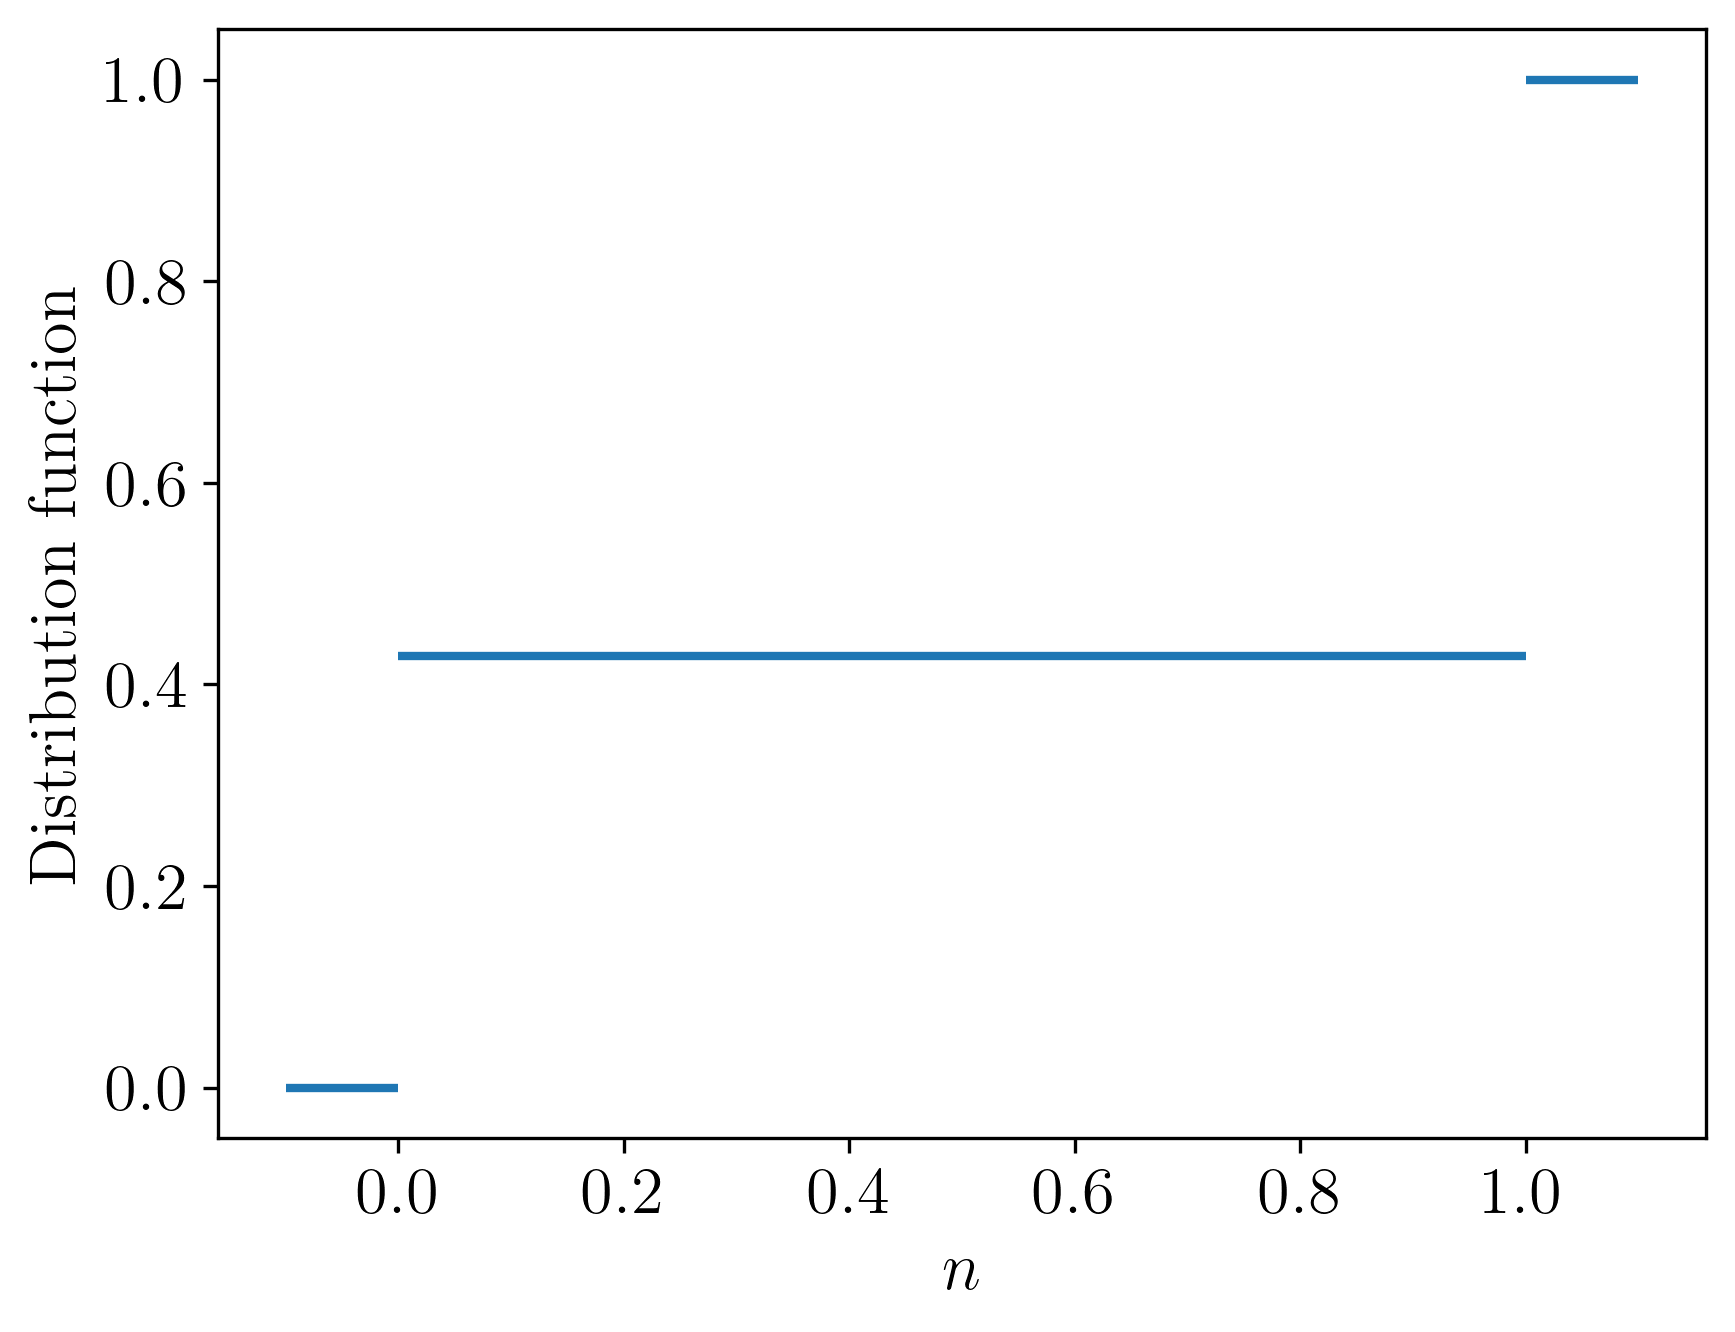
\includegraphics[width=.9\linewidth]{./Section/Grundlegende Begriffe/Verteilungsfunktion Bernoulli.png}
\vspace*{-.3\baselineskip}
\caption{\centering Verteilungsfunktion einer $\Ber(4/7)$-Verteilung}
\vspace*{-.3\baselineskip}
\end{center}
\end{figure}
\end{minipage}
\begin{minipage}{0.5\linewidth}
\begin{figure}[H]
\begin{center}
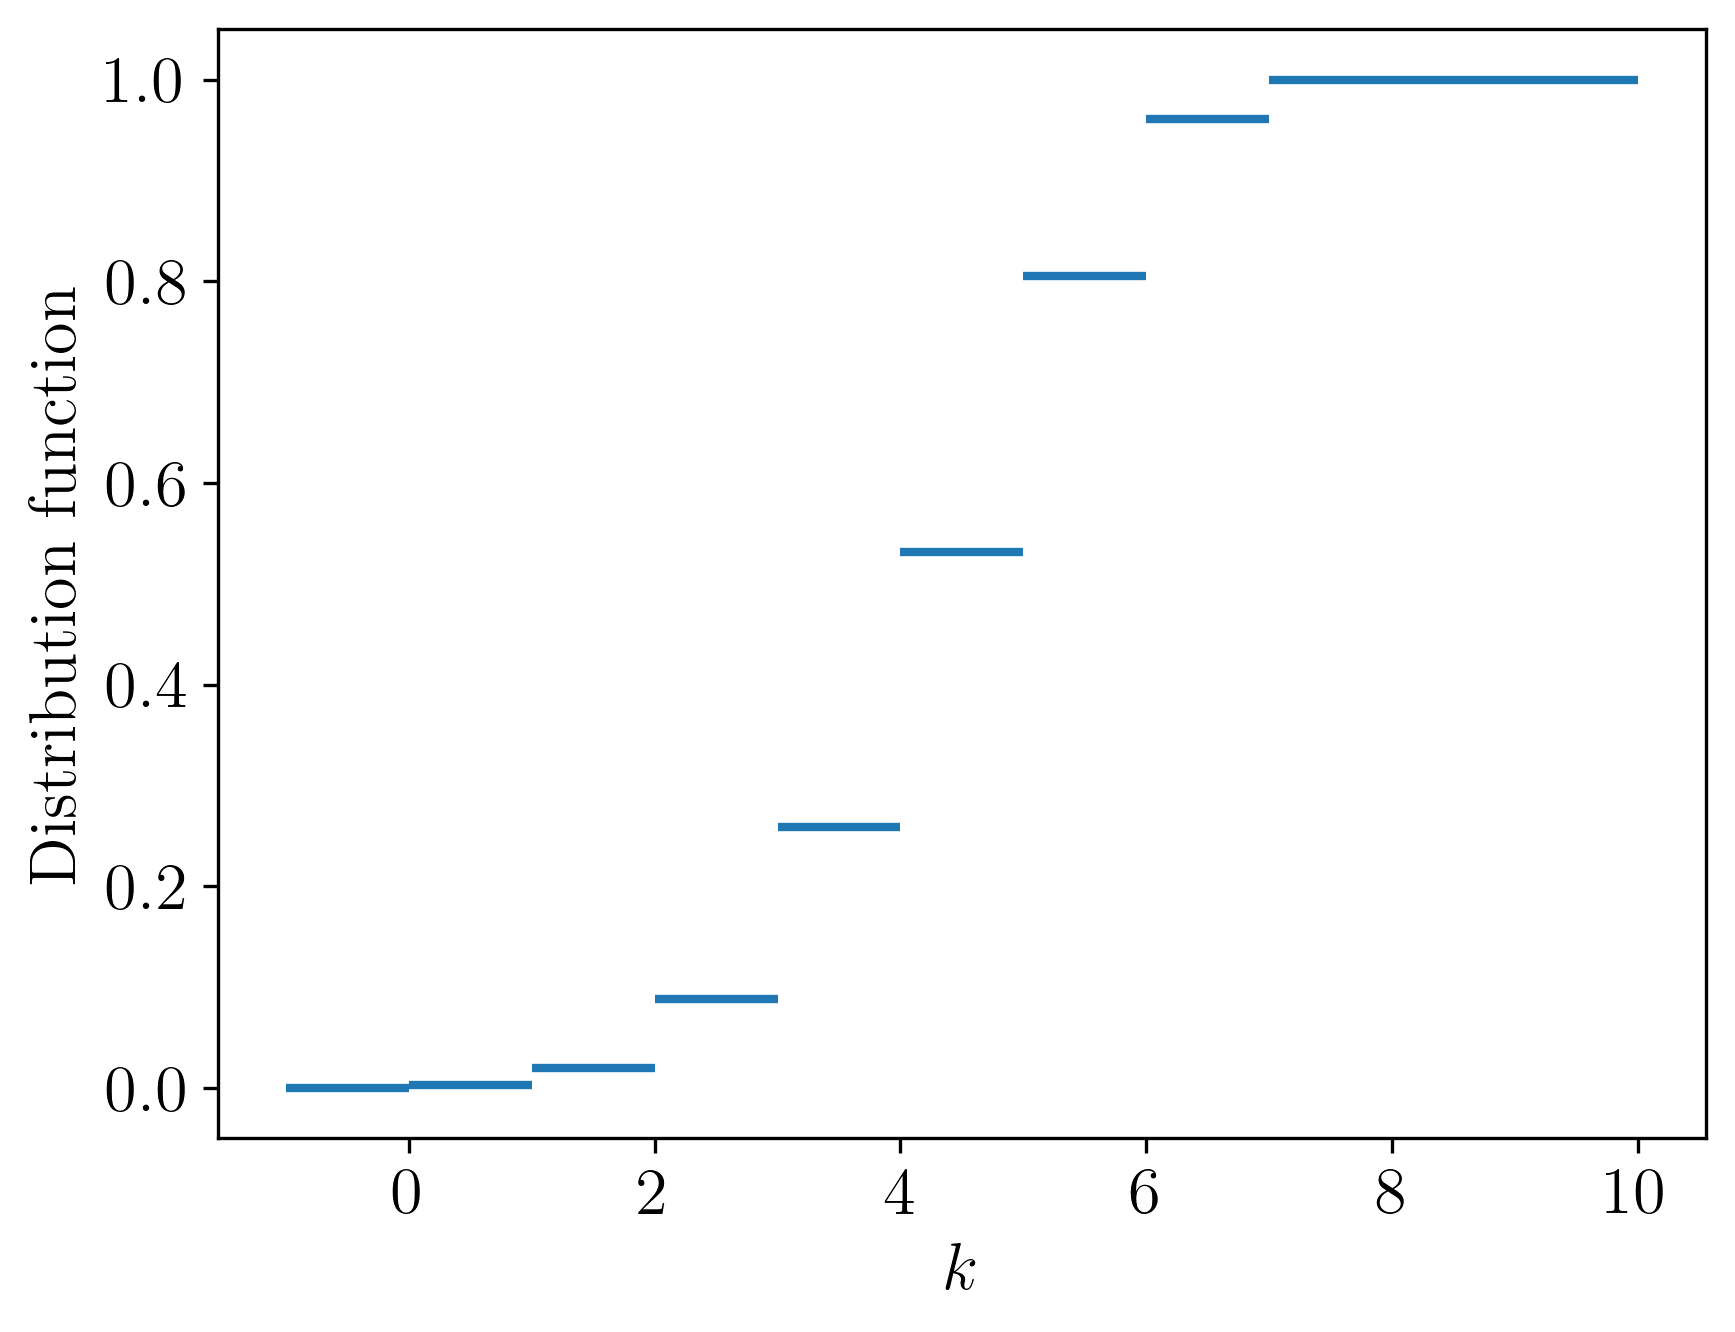
\includegraphics[width=.9\linewidth]{./Section/Grundlegende Begriffe/Verteilungsfunktion Binomial.png}
\vspace*{-.3\baselineskip}
\caption{\centering Verteilungsfunktion einer $\Bin(8, 2/3)$-Verteilung}
\vspace*{-.3\baselineskip}
\end{center}
\end{figure}
\end{minipage}
\vspace*{-\baselineskip}

\begin{minipage}{0.5\linewidth}
\begin{figure}[H]
\begin{center}
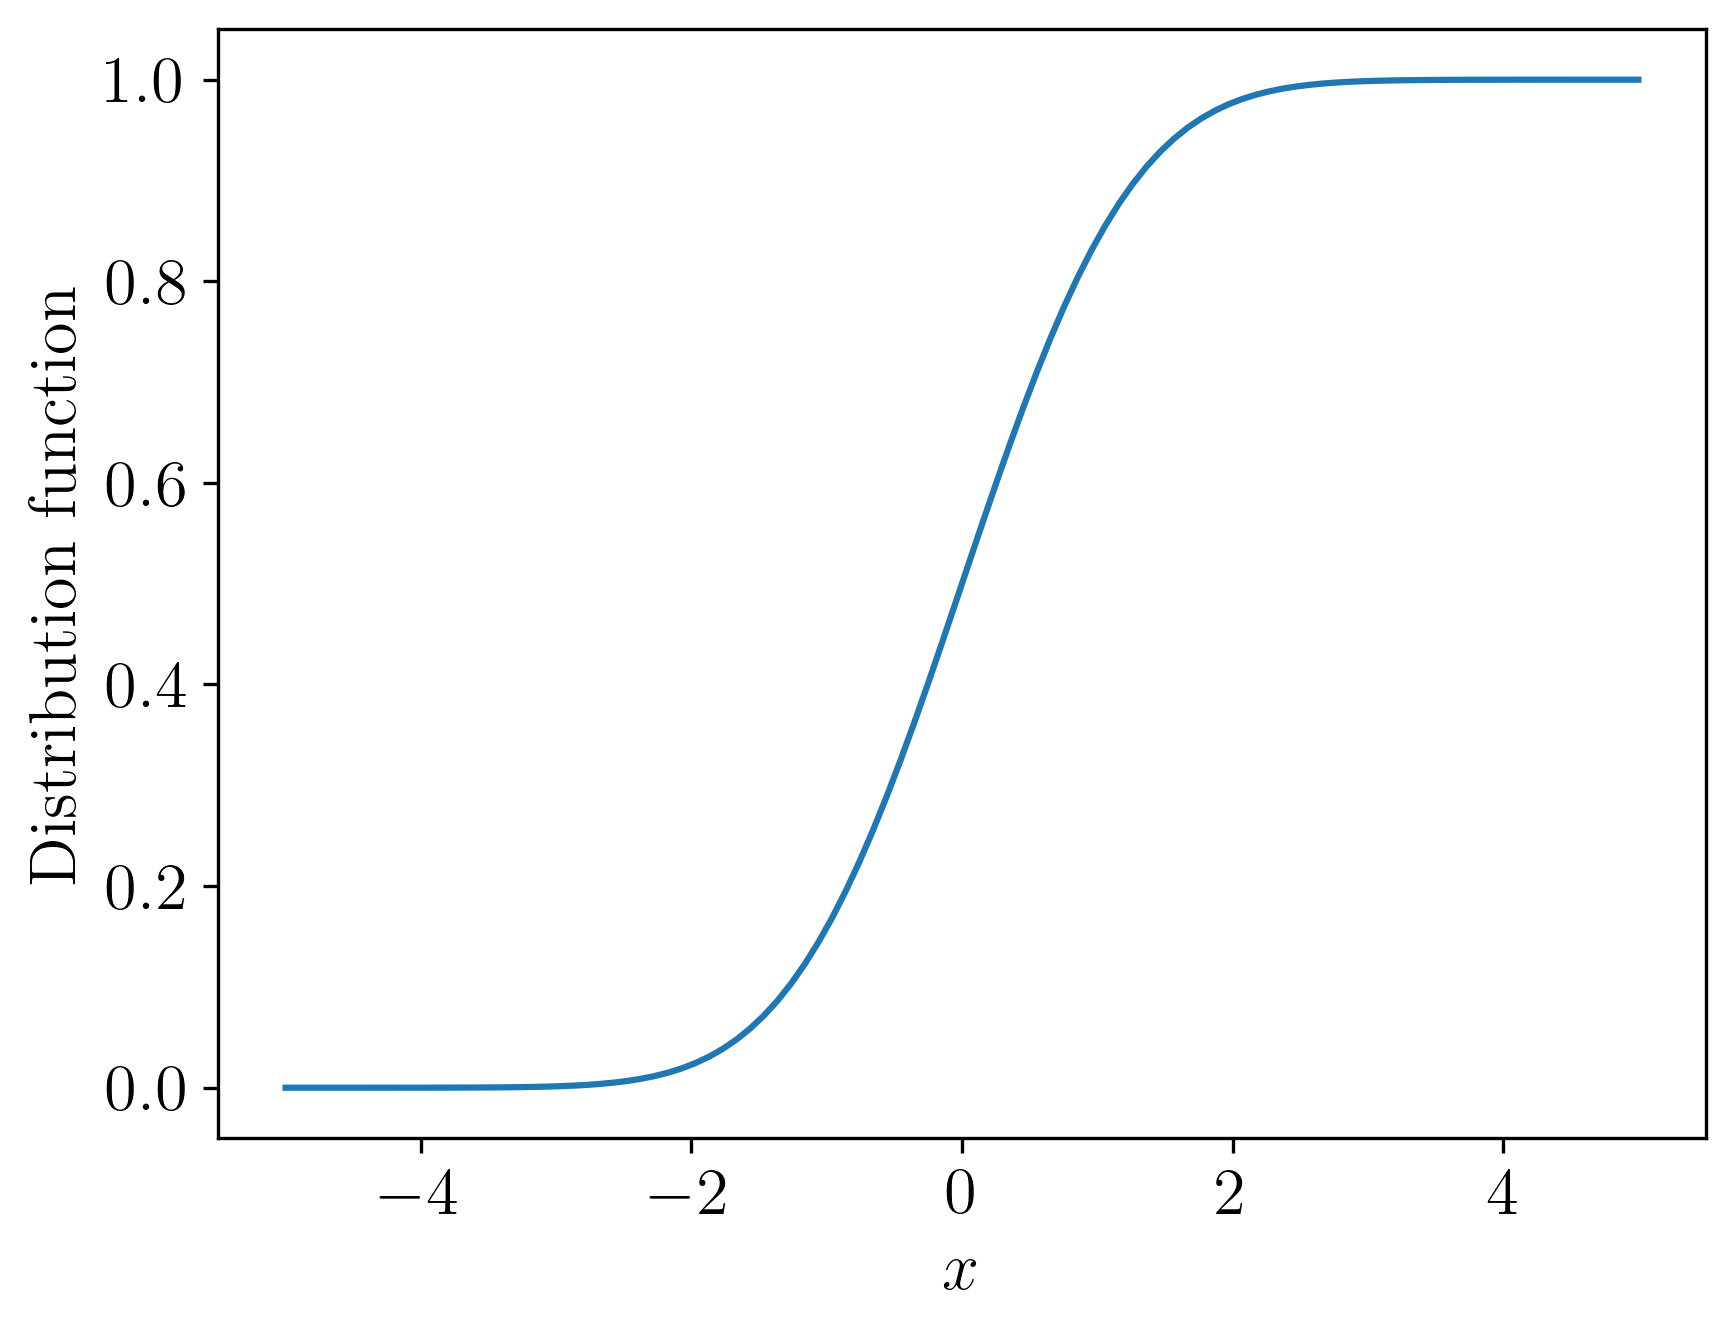
\includegraphics[width=.9\linewidth]{./Section/Grundlegende Begriffe/Verteilungsfunktion Normal.png}
\vspace*{-.3\baselineskip}
\caption{\centering Verteilungsfunktion einer $\Nor(0, 1)$-Verteilung}
\vspace*{-.3\baselineskip}
\end{center}
\end{figure}
\end{minipage}
\begin{minipage}{0.5\linewidth}
\begin{figure}[H]
\begin{center}
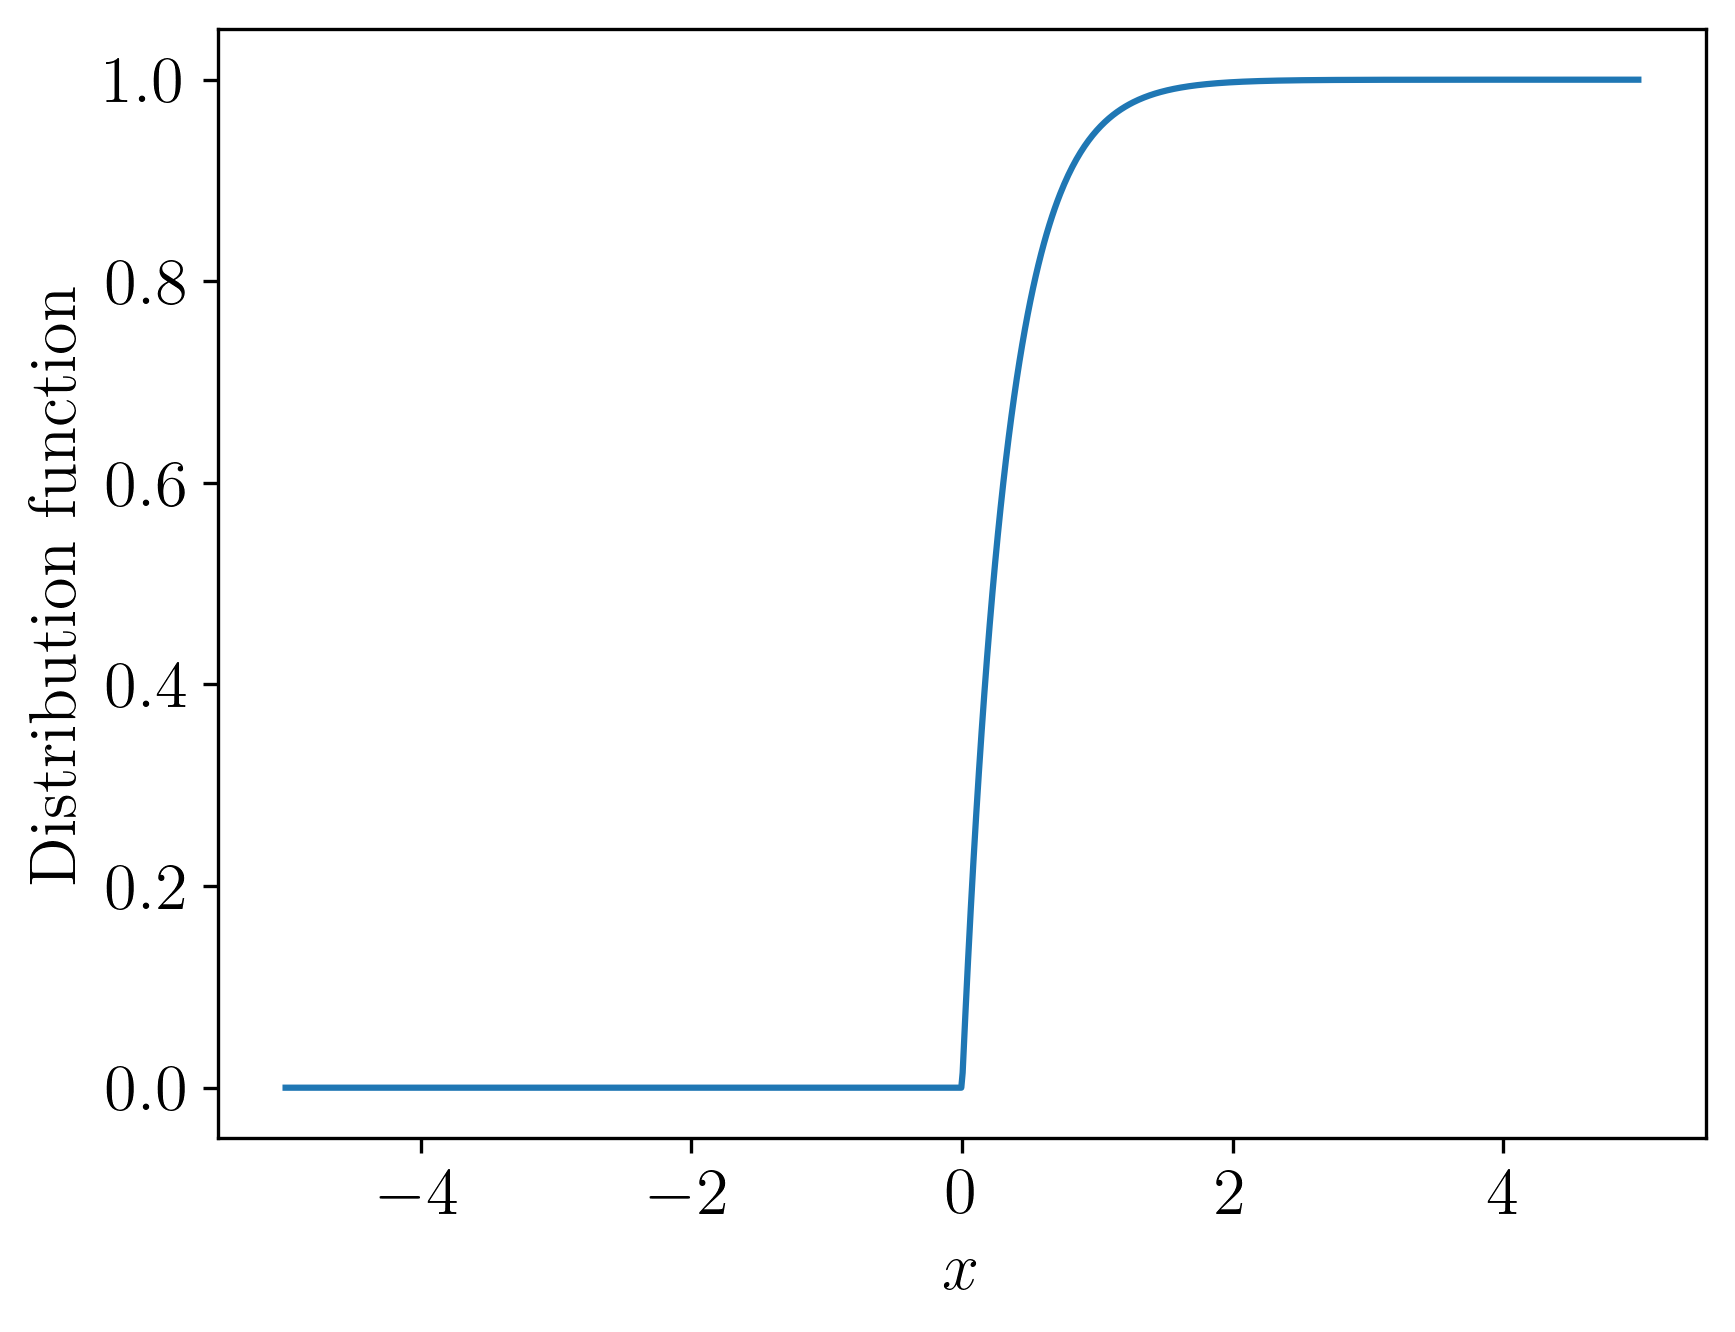
\includegraphics[width=.9\linewidth]{./Section/Grundlegende Begriffe/Verteilungsfunktion Exponential.png}
\vspace*{-.3\baselineskip}
\caption{\centering Verteilungsfunktion einer $\Exp(3)$-Verteilung}
\vspace*{-.3\baselineskip}
\end{center}
\end{figure}
\end{minipage}

Wir sehen bei allen Verteilungsfunktionen, dass sie nur Werte aus $[0, 1]$ annehmen und insbesondere die Grenzwerte $0$ und $1$ für $x \rightarrow -\infty$ und $x \rightarrow \infty$ haben. Außerdem sehen wir, dass Verteilungsfunktionen monoton wachsend sind. Bei der Bernoulli- und Binomialverteilung sehen wir deren stückweise stetige Natur. Die stetigen Verteilungen sind sogar stetig. Dies sind genau die Aussagen, die wir im \hyperlink{Satz:EigVertFun}{\blue{Satz über die Eigenschaften der Verteilungsfunktion}} gezeigt haben.
\end{Beispiel}


\setcounter{Zaehler}{0}

\section{Momente}

%In diesem Abschnitt werden wir weitere wahrscheinlichkeitstheoretische Begriffe definieren, wie Momente, Integrierbarkeit, momenterzeugende und charakteristische Funktion.

\subsection{Erwartungswerte}

Interpretiert man eine Zufallsvariable als ein Experiment mit einem zufälligen Ausgang, so könnte man sich überlegen, welche Methoden sich zur Berechnung des Erwartungswertes anbieten.

\begin{Beispiel}{(Erwartungswert Würfel)}
Wir betrachten wieder das \hyperlink{Bsp:Würfel}{\blue{Würfelbeispiel}}. Naiv würde man berechnen, dass man mit einer Wahrscheinlichkeit von $1/6$ die Zahl Eins würfelt, mit $1/6$ die Zwei und so weiter. Wir berechnen also
\[1 \cdot \frac{1}{6} + 2 \cdot \frac{1}{6} + 3 \cdot \frac{1}{6} + 4 \cdot \frac{1}{6} + 5 \cdot \frac{1}{6} + 6 \cdot \frac{1}{6} = 3.5~.\]
Ist $E = \{1, \dots, 6\}$ unser Ergebnisraum, so berechnen wir
\[\mathbb{E}(X) = \sum_{n \in E} n \mathbb{P}(X = n)~.\]
Vergleichen wir dies mit unserem \hyperlink{Kor:Dichtekorollar}{\blue{Dichtekorollar}}, so könnte man auf die Idee kommen, als zu integrierende Funktion die Identität zu wählen.
\end{Beispiel}

Dieses Beispiel erheben wir nun zur

\begin{Definition}{(Erwartungswert)}
Sei $(\Omega, \mathscr{A}, \mathbb{P})$ ein Wahrscheinlichkeitsraum und $X$ eine reelle Zufallsvariable. Der  \textit{Erwartungswert von $X$} \en{mean} ist definiert durch
\[\mathbb{E}(X) := \int X \d \mathbb{P}~.\]
\end{Definition}

Dieses Maßintegral können wir so nicht direkt berechnen.

\begin{Bemerkung}{(Berechnung des Erwartungswertes)}
\hypertarget{Bem:Berechnung_Erwartung}{}Wenden wir nun das \hyperlink{Kor:Dichtekorollar}{\blue{Dichtekorollar}} an, so erhalten wir für finite und diskrete Zufallsvariable
\begin{align*}
\mathbb{E}(X) &= \sum_{n \in \mathbb{N}_0} n \varphi(n)~.
\intertext{Für stetige Zufallsvariable erhalten wir ähnlich}
\mathbb{E}(X) &= \int_\mathbb{R} x \varphi(x) \d x~.
\end{align*}
Auf diese Weise werden wir den Erwartungswert berechnen.
\end{Bemerkung}

Mit dieser neuen Definition können wir das \hyperlink{Bsp:Regen}{\blue{Regenbeispiel}} betrachten.

\begin{Beispiel}{(Erwartungswert Regen)}
\hypertarget{Bsp:ErwRegen}{}Sei $X$ so verteilt, wie im \hyperlink{Bsp:Regen}{\blue{Regenbeispiel}}. Wir können nun berechnen, wo der Regentropfen im Mittel auftrifft. Betrachte also
\begin{align*}
\mathbb{E}(X) &= \int_\mathbb{R} x \indi_{[0, 1]}(x) \d x\\
&= \int_0^1 x \d x\\
&= \left[ \frac{x^2}{2} \right]_0^1\\
&= \frac{1}{2}~.
\end{align*}
Der Regentropfen kommt also im Mittel in der Mitte auf. Dies entspricht auch unserer Erwartung.
\end{Beispiel}

\newpage

Auf die Implementierung wollen wir im Moment noch verzichten, da wir im \hyperlink{Sec:MomGenFun}{\blue{folgenden Kapitel}} eine allgemeinere Methode zur Momentebestimmung definieren werden. Außerdem werden wir in einem \hyperlink{Sec:MomErzFun}{\blue{späteren Kapitel}} noch eine zweite Methode zur Berechnung der Momente finden.

\begin{Beispiel}{(Interpretation Erwartungswert)}
\hypertarget{Bsp:InterpretErw}{}Wie wir gerade bemerkt haben, scheint der Erwartungswert den durchschnittlichen Wert einer Zufallsvariable zu beschreiben. Den Erwartungswert können wir beispielsweise in der Dichtefunktion visualisieren. Hierfür verwenden wir die \hyperlink{Bsp:DichteBild}{\blue{Beispiele}}, für die wir die Dichtefunktion bereits visualisiert haben.\\
\begin{minipage}{0.5\linewidth}
\begin{figure}[H]
\begin{center}
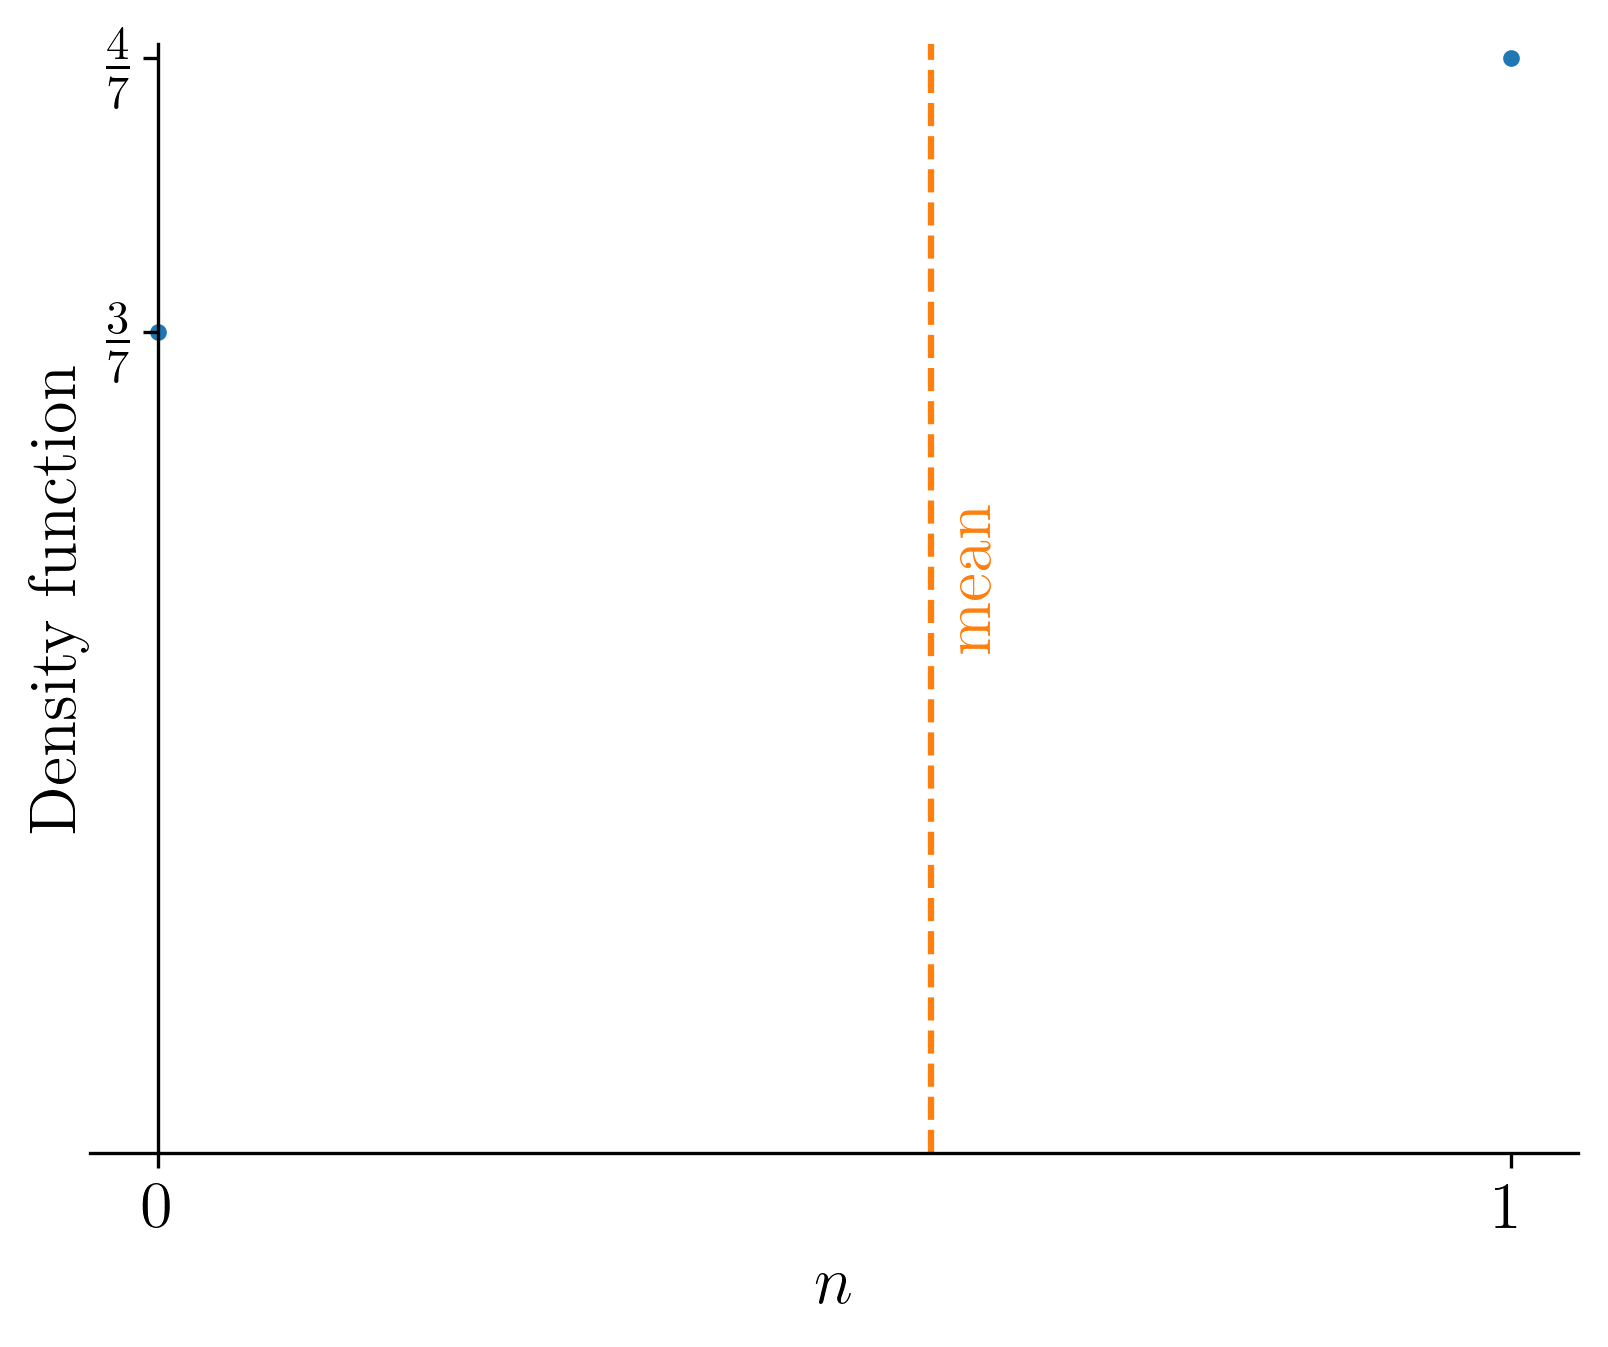
\includegraphics[width=\linewidth]{./Section/Momente/Erwartungswert Bernoulli.png}
\caption{\centering Dichte einer $\Ber(4/7)$-Verteilung}
\end{center}
\end{figure}
\end{minipage}
\begin{minipage}{0.5\linewidth}
\begin{figure}[H]
\begin{center}
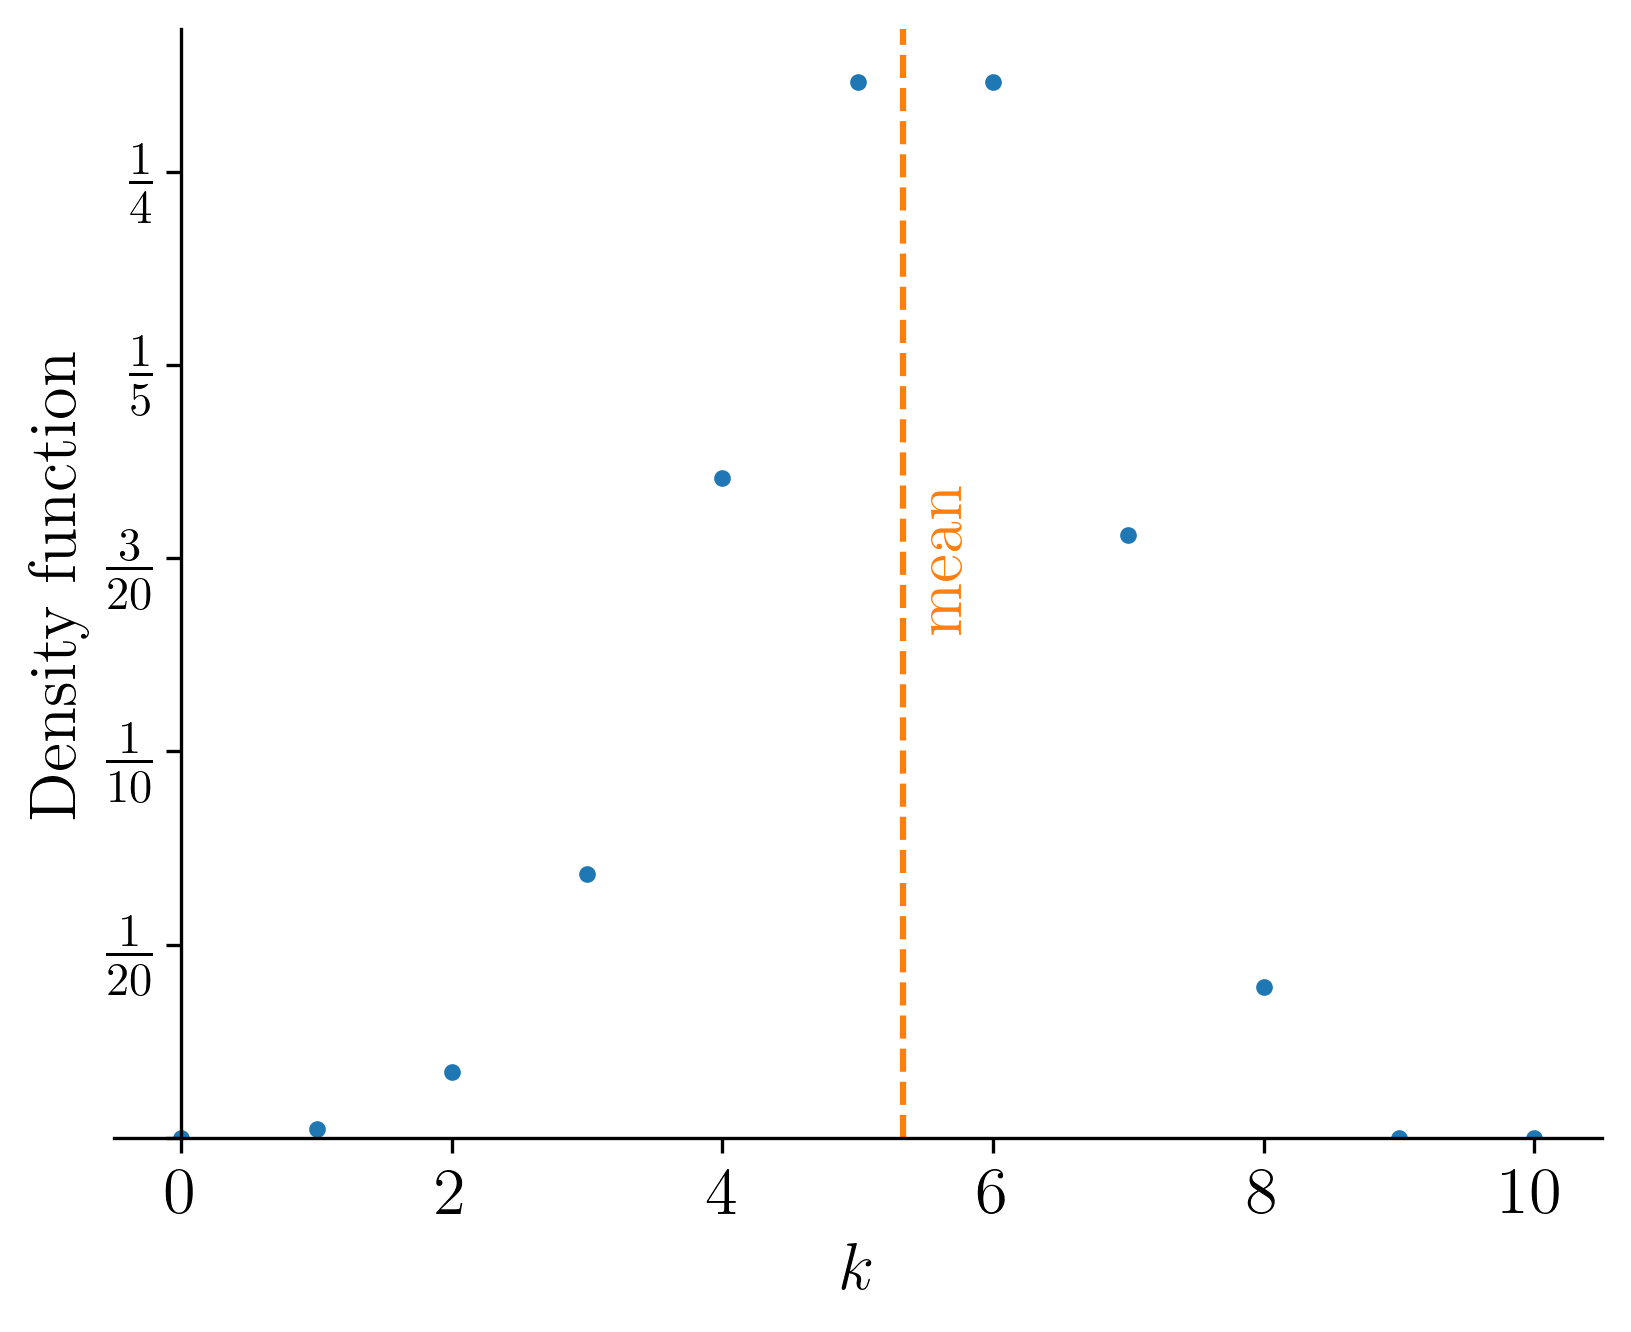
\includegraphics[width=\linewidth]{./Section/Momente/Erwartungswert Binomial.png}
\caption{\centering Dichte einer $\Bin(8, 2/3)$-Verteilung}
\end{center}
\end{figure}
\end{minipage}
\begin{minipage}{0.5\linewidth}
\begin{figure}[H]
\begin{center}
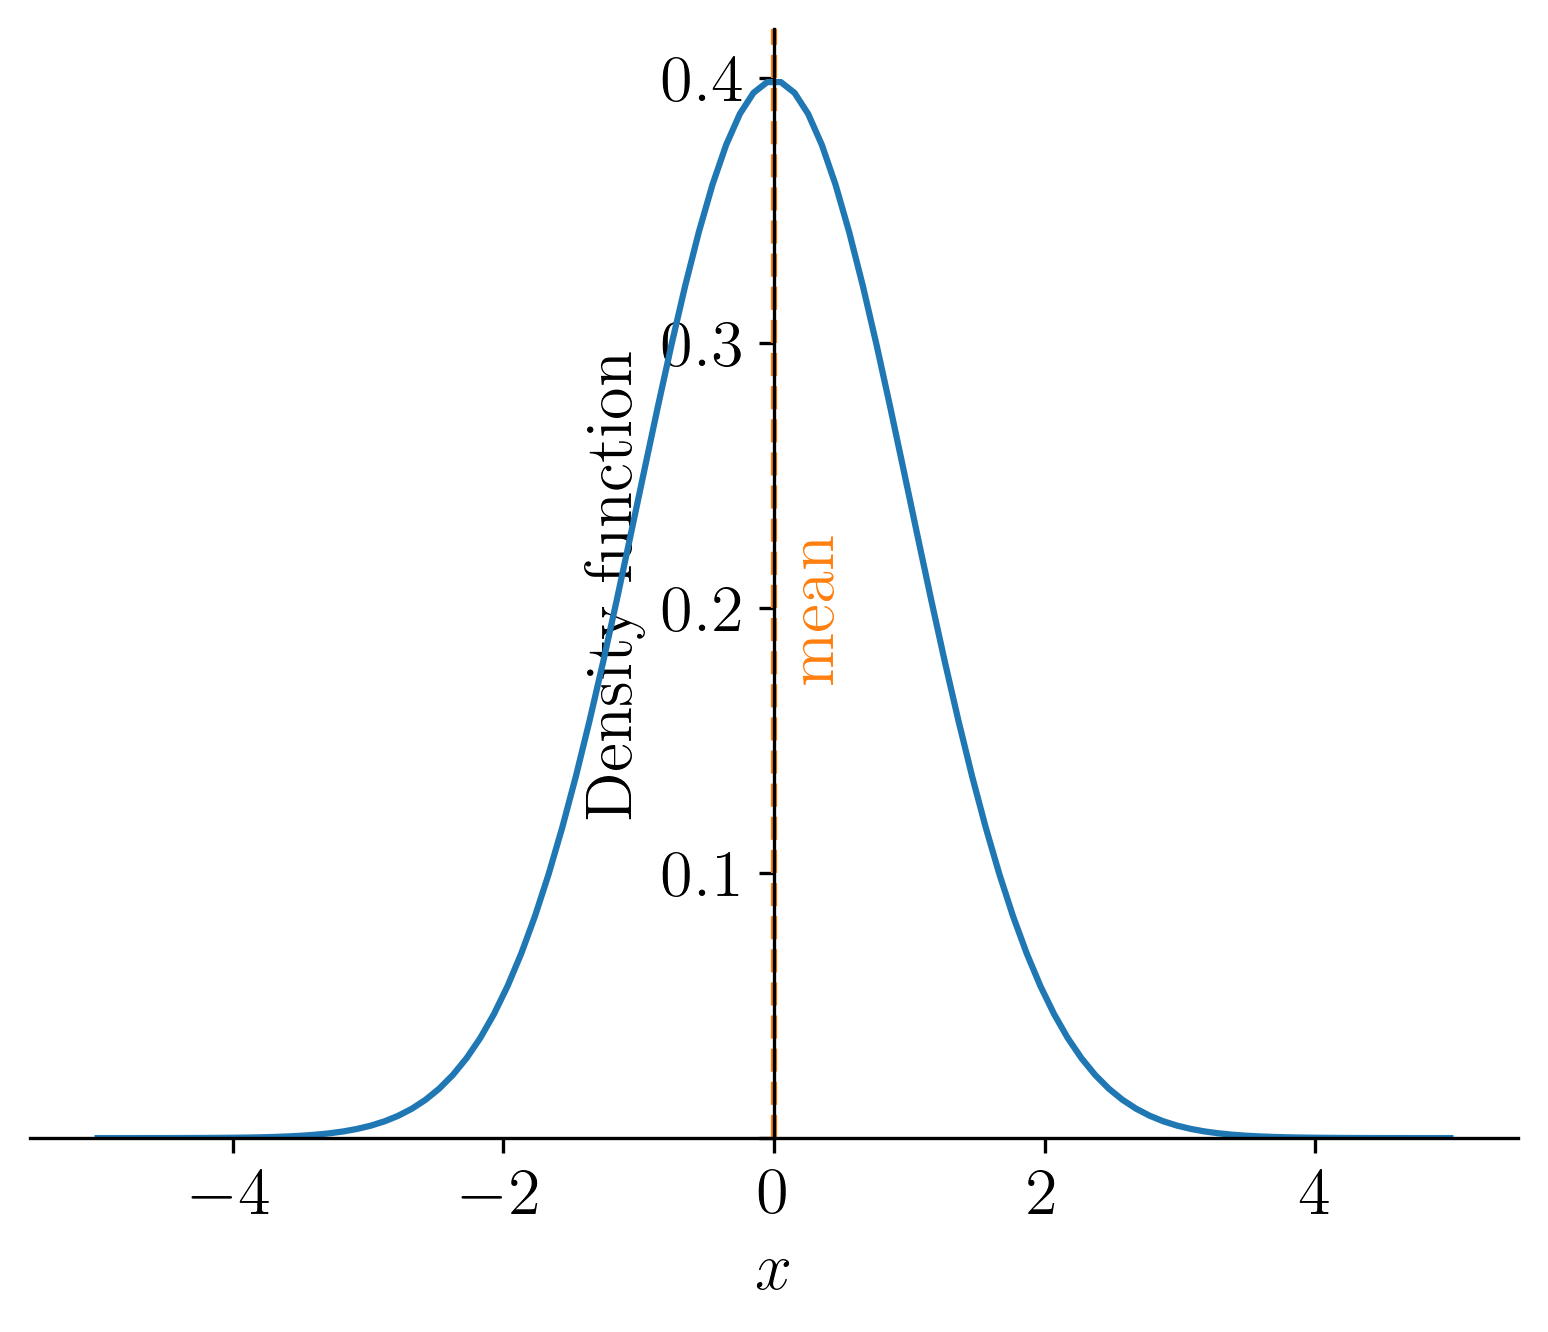
\includegraphics[width=\linewidth]{./Section/Momente/Erwartungswert Normal.png}
\caption{\centering Dichte einer $\Nor(0, 1)$-Verteilung}
\end{center}
\end{figure}
\end{minipage}
\begin{minipage}{0.5\linewidth}
\begin{figure}[H]
\begin{center}
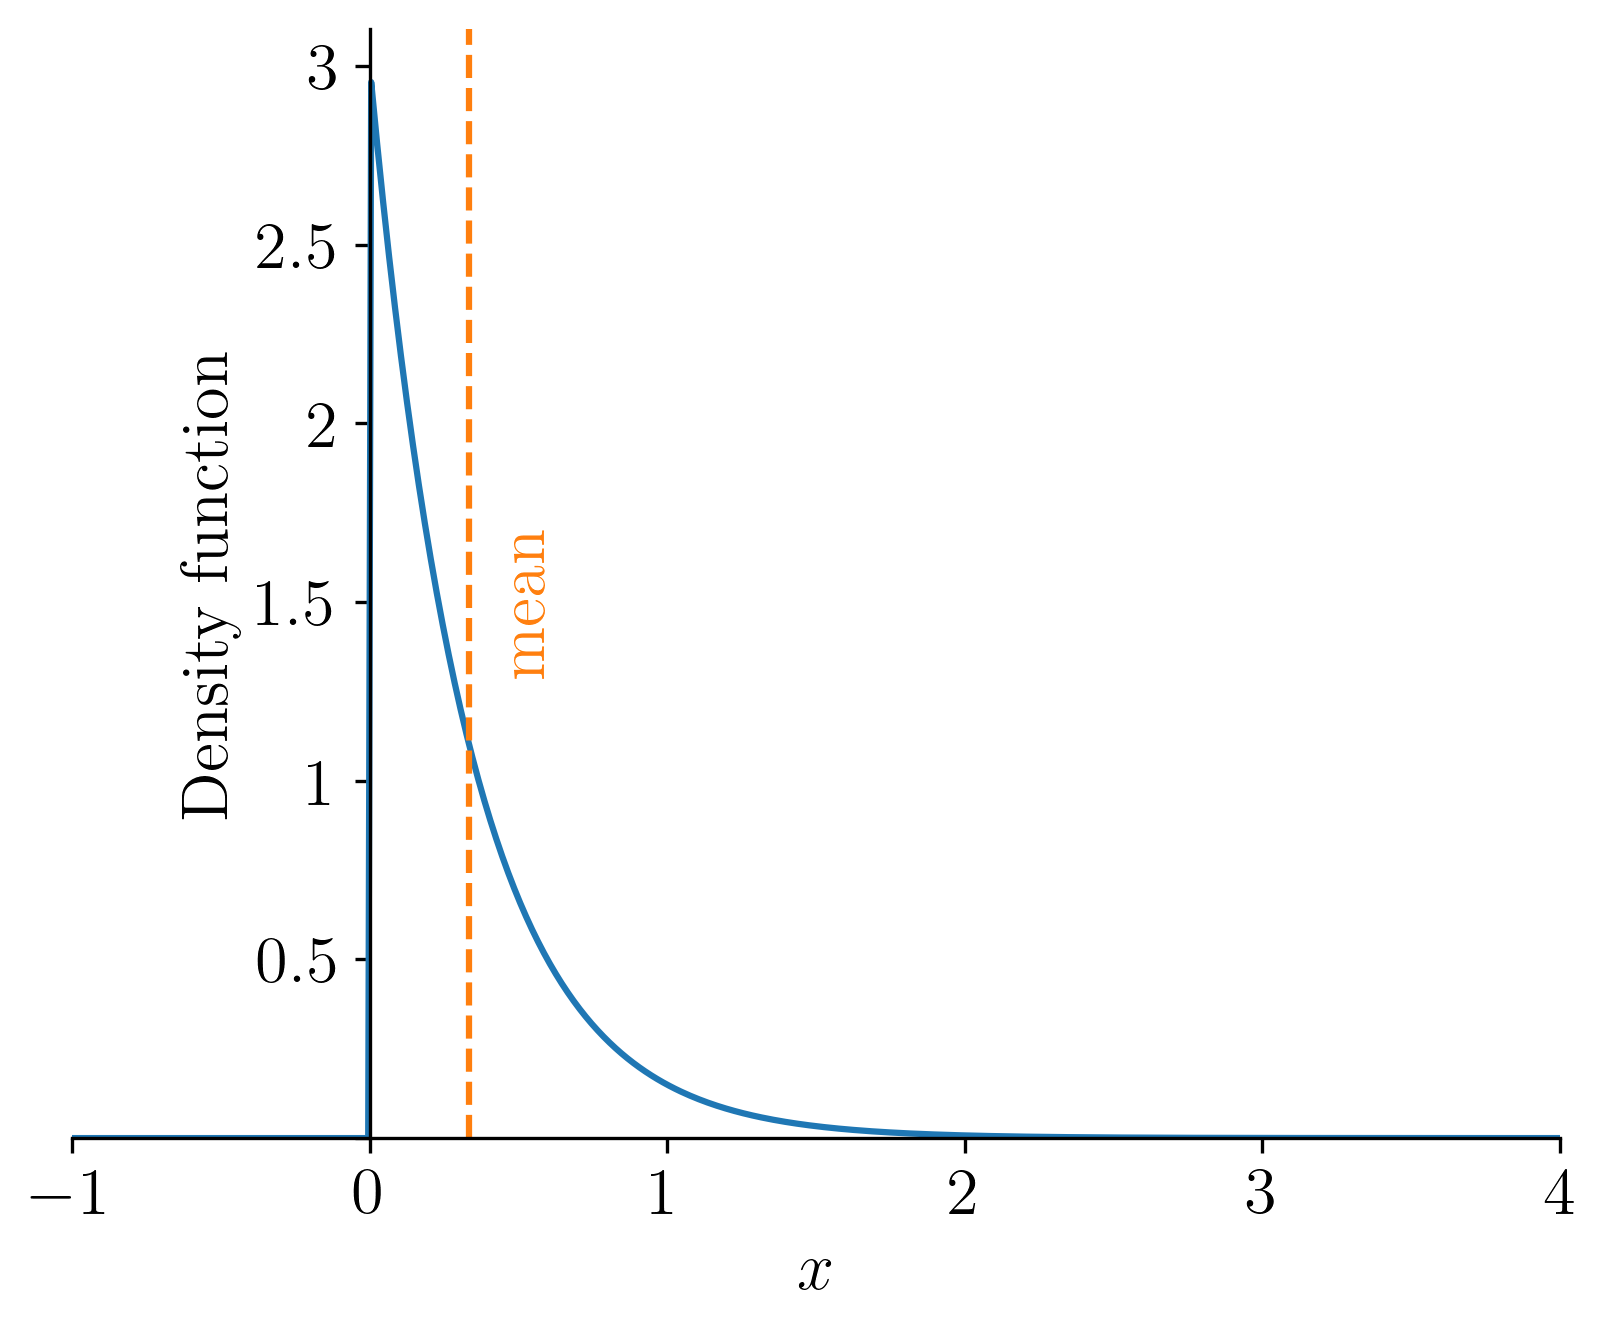
\includegraphics[width=\linewidth]{./Section/Momente/Erwartungswert Exponential.png}
\caption{\centering Dichte einer $\Exp(3)$-Verteilung}
\end{center}
\end{figure}
\end{minipage}

Wir sehen, dass der Erwartungswert tatsächlich die Verteilung teilt. Bei der finiten und diskreten Verteilung fällt auf, dass der Erwartungswert nicht unbedingt ein Wert sein muss, den die Zufallsvariable tatsächlich annimmt. Hierzu könnte man den Median \en{median} oder Modus \en{mode} berechnen.

\newpage 

Da die Dichtefunktionen von Normalverteilungen symmetrisch um den Erwartungswert sind, wollen wir diese noch gesondert betrachten.

\begin{figure}[H]
\centering
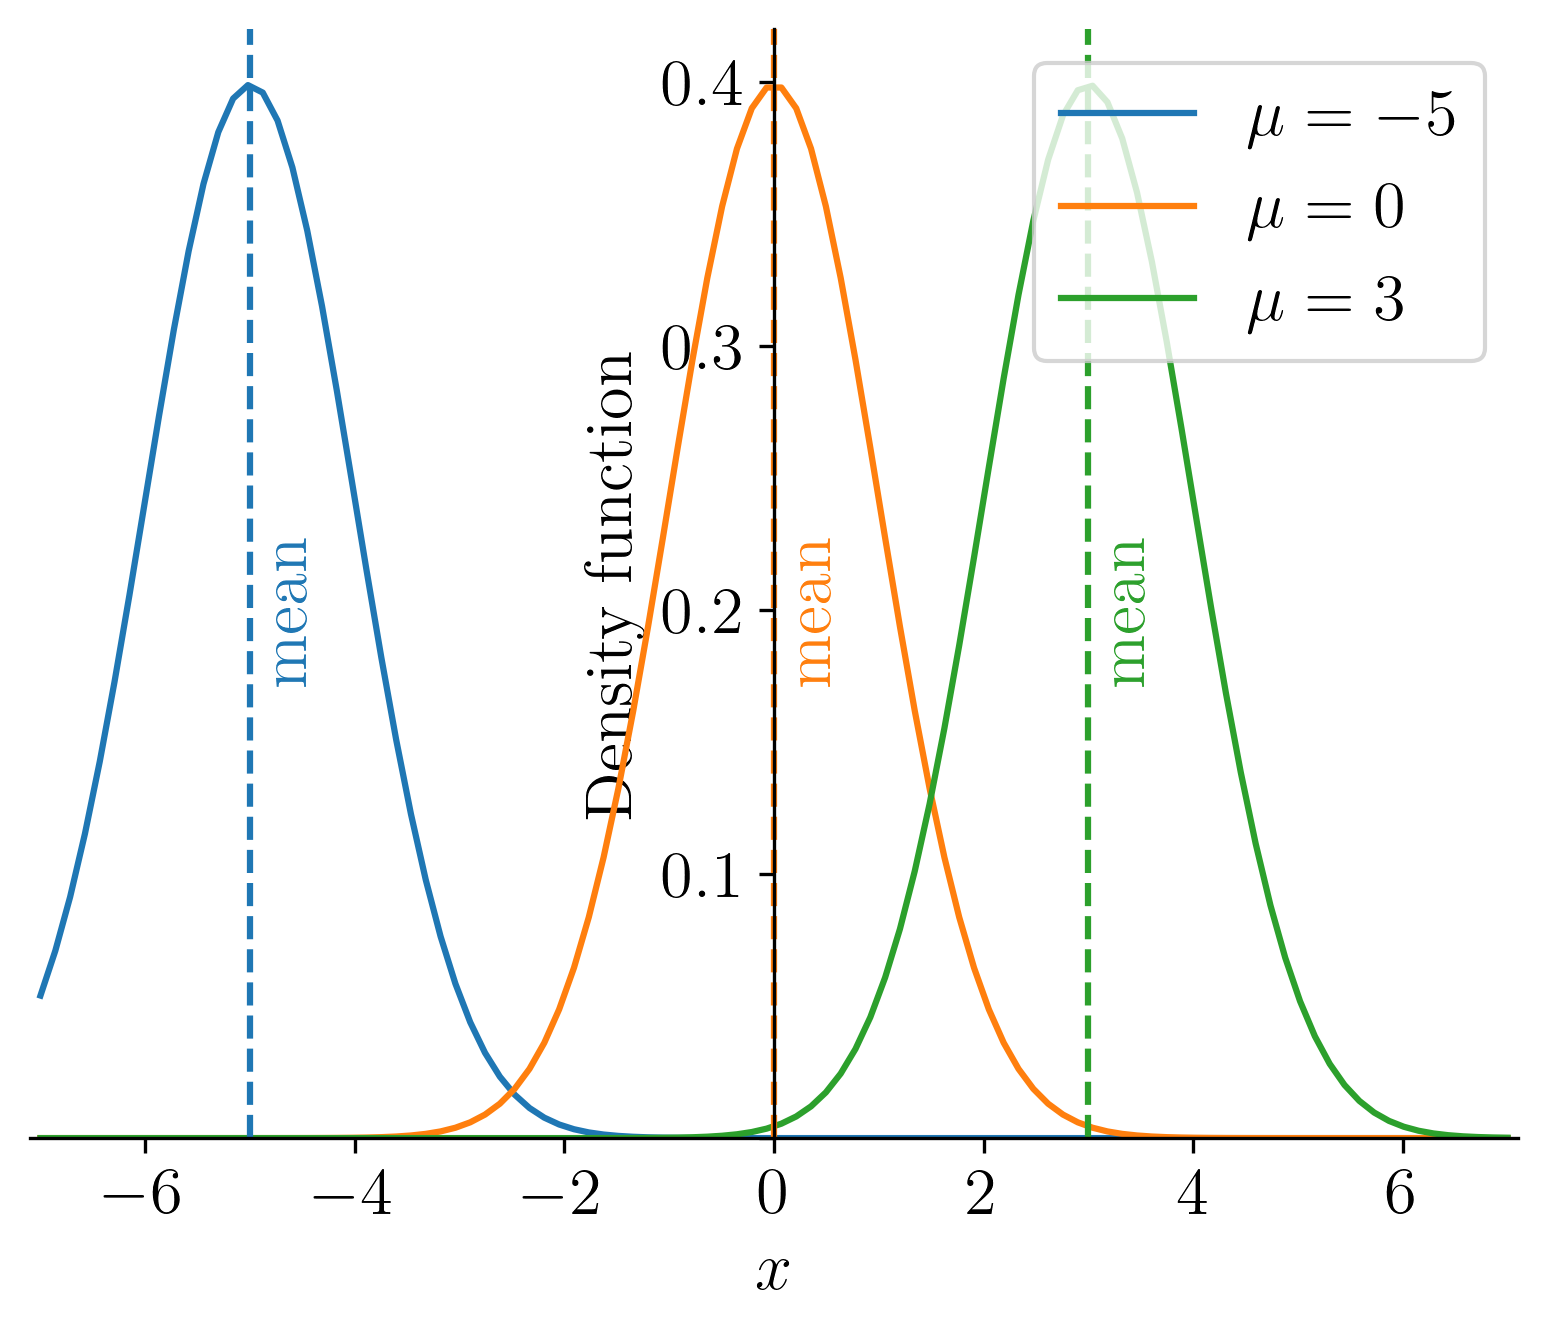
\includegraphics[width=0.5\linewidth]{./Section/Momente/Erwartungswert Normal Multi.png}
\caption{Dichte einer $\Nor(\mu, 1)$-Verteilung}
\end{figure}

Wir sehen also, dass Symmetriezentrum und Erwartungswert bei diesen Normalverteilungen zusammenfallen. Diese Aussage gilt sogar allgemein.
\end{Beispiel}

\vspace*{-\medskipamount}

\begin{Satz}{(Erwartungswert symmetrischer Verteilungen)}
Sei $(\Omega, \mathscr{A}, \mathbb{P})$ ein Wahrscheinlichkeitsraum und $X$ eine integrierbare Zufallsvariable, sodass die Dichte symmetrisch um $\mu$ ist. Dann gilt
\[\mathbb{E}(X) = \mu~.\]
\end{Satz}

\begin{Beweis}{}
Aufgrund der Symmetrie gilt
\[f(\mu + x) = f(\mu - x)\]
für alle $x \in \mathbb{R}$. Nach Definition gilt
\begin{align*}
\mathbb{E}(X) &= \int X \d \mathbb{P}\\
&= \int_\mathbb{R} x f(x) \d x~.
\intertext{Aufgrund der Integrierbarkeit können wir dieses Integral am Symmetriezentrum trennen und es gilt}
&= \int_{-\infty}^\mu x f(x) \d x + \int_\mu^\infty x f(x) \d x~.
\end{align*}
Wir werden nun diese beiden Integral getrennt voneinander betrachten. Betrachte zunächst
\begin{align*}
\int_{-\infty}^\mu x f(x) \d x &= \int_{-\infty}^\mu (\mu - (\mu - x)) f(x) \d x\\
&= \int_{-\infty}^\mu \mu f(x) - (\mu - x) f(x) \d x~.
\intertext{Dank der Linearität folgt}
&= \mu \int_{-\infty}^\mu f(x) \d x - \int_{-\infty}^\mu (\mu - x) f(x) \d x~.
\intertext{Das Integral im vorderen Summanden können wir auch mittels der Verteilungsfunktion $F_X$ ausdrücken}
&= \mu F_X(\mu) - \int_{-\infty}^\mu (\mu - x) f(x) \d x~.
\intertext{Auf eine ähnliche Weise betrachten wir das andere Integral}
\int_\mu^\infty x f(x) \d x &= \int_\mu^\infty (\mu + (x - \mu)) f(x) \d x\\
&= \int_\mu^\infty \mu f(x) + (x - \mu) f(x) \d x~.
\intertext{Mithilfe der Linearität folgt wieder}
&= \mu \int_\mu^\infty f(x) \d x + \int_\mu^\infty (x - \mu) f(x) \d x~.
\intertext{Im vorderen Integral finden wir die Gegenwahrscheinlichkeit zu vorigem Ereigniss. Wir können dies also umschreiben zu}
&= \mu (1 - F_X(\mu)) + \int_\mu^\infty (x - \mu) f(x) \d x~.
\end{align*}
Setzen wir diese Rechnung nun in die Berechnung des Erwartungswertes ein, so erhalten wir
\begin{align*}
\mathbb{E}(X) &= \mu F_X(\mu) - \int_{-\infty}^\mu (\mu - x) f(x) \d x + \mu (1 - F_X(\mu)) + \int_\mu^\infty (x - \mu) f(x) \d x\\
&= \mu - \int_{-\infty}^\mu (\mu - x) f(x) \d x + \int_\mu^\infty (x - \mu) f(x) \d x~.
\intertext{Aufgrund der Symmetrie der Dichtefunktion sind die beiden Integrale gleich und es gilt}
&= \mu~.
\end{align*}

Wir können diesen Satz auch auf eine deutlich elegantere und kürzere Art beweisen. Da $X$ symmetrisch bezüglich $\mu$ ist, haben $X - \mu$ und $\mu - X$ dieselbe Verteilung. Es gilt also
\[\mathbb{E}(X - \mu) = \mathbb{E}(\mu + X)~.\]
Damit gilt
\begin{align*}
0 &= \mathbb{E}(X - \mu) - \mathbb{E}(\mu - X)\\
&= \mathbb{E}(X - \mu - \mu + X)\\
&= \mathbb{E}(2 X - 2 \mu)\\
&= 2 \mathbb{E}(X) - 2 \mu\\
\intertext{und}
\mathbb{E}(X) &= \mu
\end{align*}
durch Umformen.
\end{Beweis}

\input{./Section/Momente/Höhere Momente.tex}

\subsection{Momenterzeugende Funktionen}
\hypertarget{Sec:MomErzFun}{}Wir beginnen dieses Kapitel mit der folgenden

\begin{Definition}{(Momenterzeugende Funktion)}
Sei $(\Omega, \mathscr{A}, \mathbb{P})$ ein Wahrscheinlichkeitsraum und $X$ eine reelle Zufallsvariable. Die \textit{momenterzeugende Funktion von $X$} \en{moment-generating function} ist definiert durch
\[M_X(t) := \mathbb{E}\left( \exp(t X) \right)~.\]
Insbesondere ist $M_X: \mathbb{D} \rightarrow \mathbb{R}: t \mapsto M_X(t)$ für $\mathbb{D} := \{ t \in \mathbb{R} \mid M_X(t) < \infty\}$ eine Abbildung.
\end{Definition}

\newpage

Wir werden nun die momenterzeugende Funktion implementieren.

\begin{Code}{(\lstinline|moment_generating_function|)}
Dank der allgemeinen Integrationsmethode ist auch an dieser Stelle nicht viel zu implementieren.
\begin{lstlisting}
def moment_generating_function(self):
    if hasattr(self, 'MGF'):
        moment_generating_function = self.MGF
    else:
        t = sym.Symbol('t', real=True)
        moment_generating_function = self.integrate_random_variable(sym.exp(t * self.variable))
        self.MGF = moment_generating_function
    return moment_generating_function
\end{lstlisting}
Neu ist, dass wir zuvor noch das Symbol \lstinline|t| definieren müssen. Da dieses Symbol hier verwendet wird, sollte man in der Definition seiner Dichtefunktion kein \lstinline|t| verwenden, da dies sonst zu großen Schwierigkeiten führt. Weiter prüfen wir zuerst, ob das Attribut \lstinline|MGF| schon belegt ist. In diesem Attribut wird die momenterzeugende Funktion nach der ersten Berechnung gespeichert, um Berechnungen zu beschleunigen.\\

Zur momenterzeugenden Funktion gibt es auch eine Visualisierungsmethode. Diese ist unter \lstinline|plot_moment_generating_function| zu finden und funktioniert wie \hyperlink{Code:PlotDensity}{\blue{\lstinline|plot_denisty|}} für stetige Zufallsvariablen. Auf Beispiele zur Visualisierung wollen wir verzichten.\\

Um zu zeigen, wieso in der Dichte kein \lstinline|t| verwendet werden sollte, definieren wir beispielsweise folgendermaßen eine Exponentialverteilung
\begin{lstlisting}[numbers=left, numberstyle=\tiny\color{codegray}]
t = sym.Symbol('t', real=True)
lamda = sym.Symbol('lamda', real=True, positive=True)
density = lamda * sym.exp(- lamda * t)
rv = RandomVariableContinuous(density, t, [sym.Integer(0), sym.oo])
moment_generating_function = rv.moment_generating_function()
\end{lstlisting}
SymPy liefert uns \lstinline|lamda*Integral(exp(t**2)*exp(-lamda*t), (t, 0, oo))| für die momenterzeugende Funktion. Dieses Integral kann SymPy nicht berechnen, da es aufgrund des $t^2$ Terms divergiert. Wir werden im folgenden Beispiel die richtige momenterzeugende Funktion berechnen.
\end{Code}

\vspace*{-\medskipamount}

\begin{Bemerkung}{(Momenterzeugende Funktion in Null)}
\hypertarget{Bem:MomGenFun_Null}{}Sei $X$ eine reelle Zufallsvariable und $M_X$ eine um Null existierende momenterzeugende Funktion. Betrachte
\begin{align*}
M_X(0) &= \mathbb{E}(\exp(0 \cdot x))\\
&= \mathbb{E}(\exp(0))\\
&= \mathbb{E}(1)\\
&= \int 1 \d \mathbb{P}~.
\intertext{Da $\mathbb{P}$ ein Wahrscheinlichkeitsmaß ist, folgt aus der Normiertheit}
&= 1~.
\end{align*}
Dies werden wir später noch benötigen. Diese Aussage können wir wieder mit SymPy \glqq beweisen\grqq{}. Mit
\begin{lstlisting}[numbers=left, numberstyle=\tiny\color{codegray}]
x = sym.Symbol('x', real=True)
t = sym.Symbol('t', real=True)
f = sym.Function('f')(x)
rv = RandomVariableContinuous(f, x, force_density=True)
moment_generating_function = rv.moment_generating_function()
value = moment_generating_function.subs(t, sym.Integer(0))
\end{lstlisting}
erhalten wir \lstinline|Integral(f(x), (x, -oo, oo))|, was eins ist.
\end{Bemerkung}

Wir werden nun einige Beispiele für momenterzeugende Funktionen berechnen.

\begin{Beispiel}{(Momenterzeugende Funktionen)}
\hypertarget{Bsp:Moment_Erz}{}
\begin{enumerate}[label=(\roman*)]
\item Sei $X \sim \Ber(p)$ mit $p \in (0, 1)$ Bernoulli-verteilt. Wir berechnen mit $E = \{0, 1\}$
\begin{align*}
M_X(t) &= \int \exp(t X) \d \mathbb{P}\\
&= \sum_{n \in E} \exp(t n) \mathbb{P}(X = n)\\
&= \exp(t \cdot 0) \mathbb{P}(X = 0) + \exp(t \cdot 1) \mathbb{P}(X = 1)\\
&= \exp(0) (1 - p) + \exp(t) p\\
&= (1 - p) + p \exp(t)~.
\end{align*}
Um dies mit dem Programm zu berechnen, verwenden wir
\begin{lstlisting}[numbers=left, numberstyle=\tiny\color{codegray}]
p = sym.Symbol('p', real=True, positive=True)
n = sym.Symbol('n', integer=True, nonnegative=True)
density = {1: p, 0: 1 - p}
rv = RandomVariableFinite(density, n)
moment_generating_function = rv.moment_generating_function()
\end{lstlisting}
und erhalten ebenfalls \lstinline|p*exp(t) - p + 1|.

\item Sei $X \sim \Exp(\lambda)$ mit $\lambda > 0$ exponentialverteilt. Wir berechnen
\begin{align*}
M_X(t) &= \int \exp(t X) \d \mathbb{P}\\
&= \int_{-\infty}^\infty \exp(t x) \lambda \exp(- \lambda x) \indi_{[0, \infty)}(x) \d x\\
&= \lambda \int_0^\infty  \exp\left( (t - \lambda) x \right) \d x\\
&= \lambda \left[ \frac{1}{t - \lambda} \exp\left( (t - \lambda) x \right) \right]_0^\infty\\
&= \lambda \left[ 0 - \frac{1}{t - \lambda} \right]\\
&= \frac{\lambda}{\lambda - t}~.
\end{align*}
Durch
\begin{lstlisting}[numbers=left, numberstyle=\tiny\color{codegray}]
x = sym.Symbol('x', real=True)
lamda = sym.Symbol('lambda', real=True, positive=True)
density = lamda * sym.exp(- lamda * x)
rv = RandomVariableContinuous(density, x, [sym.Integer(0), sym.oo])
moment_generating_function = rv.moment_generating_function()
\end{lstlisting}
erhalten wir ebenfalls \lstinline|lambda/(lambda - t)|.

\item Sei nun $X \sim \Nor(\mu, \sigma)$ mit $\mu \in \mathbb{R}$ und $\sigma > 0$ normalverteilt. 
Diese momenterzeugende Funktion wollen wir nicht von Hand berechnen, da dies ziemlich kompliziert ist. SymPy schafft dies folgendermaßen problemlos.
\begin{lstlisting}[numbers=left, numberstyle=\tiny\color{codegray}]
x = sym.symbols('x', real=True)
mu = sym.symbols('mu', real=True)
sigma = sym.symbols('sigma', real=True, positive=True)
density = 1 / (sigma * sym.sqrt(2 * sym.pi)) * sym.exp(- (x - mu)**2 / (2 * sigma**2))
rv = RandomVariableContinuous(density, x)
moment_generating_function = rv.moment_generating_function()
\end{lstlisting}
Wir erhalten \lstinline|exp(t*(mu + sigma**2*t/2))|, wie in \cite{Joram} nachzulesen ist.
\end{enumerate}
\end{Beispiel}

\newpage 

Wir werden nun einen Satz beweisen, der es uns erlaubt die momenterzeugenden Funktion als eine Potenzreihe der Momente darzustellen.

\begin{Satz}{(Potenzreihendarstellung der momenterzeugenden Funktion) \cite{Meintrup}}
\hypertarget{Satz:Potenzreihe}{}Sei $(\Omega, \mathscr{A}, \mathbb{P})$ ein Wahrscheinlichkeitsraum und $X$ eine reelle Zufallsvariable. Ist $M_X$ die momenterzeugende Funktion und existiert ein $\varepsilon > 0$, sodass $(- \varepsilon, \varepsilon) \subseteq \mathbb{D}$, so gilt
\[M_X(t) = \sum_{n = 0}^\infty \frac{t^n}{n!} \mathbb{E}(X^n)~.\]
\end{Satz}

\begin{Beweis}{\cite{Meintrup}}
Betrachte die Potenzreihe der Exponentialfunktion
\[\exp(t c) = \sum_{n = 0}^\infty \frac{t^n}{n!} c^n~.\]
Wir erkennen eine deutliche Ähnlichkeit zu dem, was wir zeigen wollen. Wir müssen also beweisen, dass wir Erwartungswert und Summation vertauschen dürfen. Sei für $N \in \mathbb{N}$ durch
\[f_N(X) := \sum_{n = 0}^N \frac{t^n}{n!} X^n\]
eine Folge von Zufallsvariablen definiert. Dann gilt nach obiger Potenzreihe
\begin{align*}
M_X(t) &= \mathbb{E}\left( \exp(t X) \right)\\
&= \mathbb{E}\left( \lim_{N \rightarrow \infty} f_N(X) \right)~.
\intertext{Da nach Definition $\exp(t X)$ überall auf $\mathbb{D}$ $\mathbb{P}_X$-integierbar ist, können wir mit dem Satz von Lebesgue Limes und Integration vertauschen und erhalten}
&= \lim_{N \rightarrow \infty} \mathbb{E}\left( f_N(X) \right)\\
&= \lim_{N \rightarrow \infty} \mathbb{E}\left( \sum_{n = 0}^N \frac{t^n}{n!} X^n \right)~.
\intertext{Dank Linearität des Erwarungswertes folgt für diese endliche Summe}
&= \lim_{N \rightarrow \infty} \sum_{n = 0}^N \frac{t^n}{n!} \mathbb{E}(X^n)\\
&= \sum_{n = 0}^\infty \frac{t^n}{n!} \mathbb{E}(X^n)~,
\end{align*}
was zu zeigen war.
\end{Beweis}
\medskip

Damit können wir nun mit der momenterzeugenden Funktion die Momente berechnen.

\begin{Korollar}{(Momente mit momenterzeugenden Funktion)}
\hypertarget{Kor:Momente_MomGenFun}{}Sei $(\Omega, \mathscr{A}, \mathbb{P})$ ein Wahrscheinlichkeitsraum und $X$ eine reelle Zufallsvariable. Ist $M_X$ die momenterzeugende Funktion und existiert ein $\varepsilon > 0$, sodass $(- \varepsilon, \varepsilon) \subseteq \mathbb{D}$, so gilt
\[\mathbb{E}(X^n) = \left[ \frac{\d^n}{\d t^n} M_X(t) \right]_{t = 0}\]
und alle Momente sind endlich.
\end{Korollar}

\begin{Beweis}{}
Betrachte zuerst
\begin{align*}
\frac{\d^n}{\d t^n} t^k = \begin{cases}
\frac{k!}{(n - k)!} t^{k - n}, &n < k\\
n!, &n = k\\
0, &n > k~.
\end{cases}
\end{align*}
Setzen wir $t = 0$ ein, so gilt
\begin{align*}
\left[ \frac{\d^n}{\d t^n} t^k \right]_{t = 0} = \begin{cases}
0, &n < k\\
n!, &n = k\\
0, &n > k~.
\end{cases}
\end{align*}
Mit dem \hyperlink{Satz:Potenzreihe}{\blue{Satz über die Potenzreihendarstellung der momenterzeugenden Funktion}} gilt
\begin{align*}
\left[ \frac{\d^n}{\d t^n} M_X(t) \right]_{t = 0} &= \left[ \frac{\d^n}{\d t^n} \sum_{k = 0}^\infty \frac{t^k}{k!} \mathbb{E}(X^k) \right]_{t = 0}~.
\intertext{Da eine Potenzreihe im inneren ihre Konvergenzradiuses unendlich oft differenzierbar ist, folgt durch Vertauschen von Differentiation und Summenbildung}
&= \left[ \sum_{k = 0}^\infty \frac{\d^n}{\d t^n} \frac{t^k}{k!} \mathbb{E}(X^k) \right]_{t = 0}~.
\intertext{Nach obiger Betrachtung bleibt nur für Summanden mit $n = k$ der Faktor $n!$ übrig. Es folgt also}
&= \frac{n!}{n!} \mathbb{E}(X^n)\\
&= \mathbb{E}(X^n)~,
\end{align*}
was zu zeigen war.
\end{Beweis}
\medskip

Dieses Korollar werden wir als Methode zur alternative Berechnung der Momente implementieren.

\begin{Code}{(\lstinline|_moment_generating|)}
\hypertarget{Code:n_Moment_Generating}{}Wir haben nun gesehen, dass wir mithilfe der momenterzeugenden Funktion die Momente einer Zufallsvariable erzeugen können. Da wir hier einige Werkzeuge von SymPy verwenden, die wir bisher noch nicht benötigt haben, wollen wir hier den Code besprechen.
\begin{lstlisting}
def _moment_generating(self, n):
    t = sym.Symbol('t', real=True)
    moment_generating_function = self.moment_generating_function()
    moment = sym.diff(moment_generating_function, (t, n))
    moment = moment.subs(t, sym.Integer(0))
    moment = sym.simplify(moment)
    return moment
\end{lstlisting}
Zuerst lassen wir uns die momenterzeugende Funktion bestimmen. Diese leiten wir mithilfe von SymPy  \lstinline|n| mal nach \lstinline|t| ab. Anschließend setzen wir für \lstinline|t| den Wert \lstinline|0| ein und versuchen dies zu vereinfachen. Es ist es wichtig in der Ableitung \lstinline|(t, n)| zu klammern, falls man für \lstinline|n| ein Symbol verwenden möchte.

\newpage

Dazu betrachten wir das folgende kurze Beispiel.
\begin{lstlisting}[numbers=left, numberstyle=\tiny\color{codegray}]
x = sym.Symbol('x', real=True)
n = sym.Symbol('n', integer=True, positive=True)
f = sym.exp(x**2)
wrong = sym.Derivative(f, x, n)
right = sym.Derivative(f, (x, n))
\end{lstlisting}
Die \lstinline|Derivative|-Methode ist eine noch nicht ausgeführte Version der \lstinline|diff| Methode. Wir erhalten im ersten Fall
\[\frac{\d^2}{\d x \d n} \exp(x^2)~,\]
was wir nicht wollen und im zweiten Fall
\[\frac{\d^n}{\d x^n} \exp(x^2)~.\] 
Mit dieser Methode ist es leider nicht möglich das allgemeine $n$-te Moment zu berechnen, da SymPy  keine Funktion $n$-mal ableiten möchte. Selbst
\begin{lstlisting}[numbers=left, numberstyle=\tiny\color{codegray}]
x = sym.Symbol('x', real=True)
n = sym.Symbol('n', integer=True, postive=True)
expr = sym.exp(x)
derivative = sym.diff(expr, (x, n))
\end{lstlisting}
bleibt unevaluiert.
\end{Code}

Mithilfe dieser neuen Methode werden wir nun einige Momente berechnen.

\begin{Beispiel}{(Momente mit momenterzeugenden Funktionen)}
Wir verwenden die momenterzeugenden Funktionen aus \hyperlink{Bsp:Moment_Erz}{\blue{obigem Beispiel}}
\begin{enumerate}[label=(\roman*)]
\item Sei $X \sim \Ber(p)$ mit $p \in (0, 1)$ Bernoulli-verteilt. Die momenterzeugende Funktion ist dann
\[M_X(t) = (1 - p) + p \exp(t)~.\]
Wir berechnen beispielsweise das vierte Moment
\begin{align*}
\mathbb{E}(X^4) &= \left[ \frac{\d^4}{\d t^4} M_X(t) \right]_{t = 0}\\
&= \left[ \frac{\d^4}{\d t^4} (1 - p) + p \exp(t) \right]_{t = 0}~.
\intertext{Der erste Summand fällt beim Ableiten weg, da dort kein $t$ vorkommt und der hintere verändert sich nicht. Somit gilt}
&= \left[ p \exp(t) \right]_{t = 0}\\
&= p \exp(0)\\
&= p
\end{align*}
Verwenden wir
\begin{lstlisting}[numbers=left, numberstyle=\tiny\color{codegray}]
p = sym.Symbol('p', real=True, positive=True)
n = sym.Symbol('n', integer=True, nonnegative=True)
density = {1: p, 0: 1 - p}
rv = RandomVariableFinite(density, n)
fourth_moment = rv._moment_generating(4)
\end{lstlisting}
so erhalten wir ebenfalls \lstinline|p|.

\item Sei $X \sim \Exp(\lambda)$ mit $\lambda > 0$ exponentialverteilt. Die momenterzeugende Funktion ist
\[M_X(t) = \frac{\lambda}{\lambda - t}~.\]
Wir berechnen das zweite Moment
\begin{align*}
\mathbb{E}(X^2) &= \left[ \frac{\d^2}{\d t^2} M_X(t) \right]_{t = 0}\\
&= \left[ \frac{\d^2}{\d t^2} \frac{\lambda}{\lambda - t} \right]_{t = 0}~.
\intertext{Einmal Ableiten liefert}
&= \left[ \frac{\d}{\d t} \frac{\lambda}{(\lambda - t)^2} \right]_{t = 0}
\intertext{und nochmal Ableiten liefert dann}
&= \left[ \frac{2 \lambda}{(\lambda - t)^3} \right]_{t = 0}\\
&= \frac{2 \lambda}{(\lambda - 0)^3}\\
&= \frac{2}{\lambda^2}~.
\end{align*}
Durch
\begin{lstlisting}[numbers=left, numberstyle=\tiny\color{codegray}]
x = sym.Symbol('x', real=True)
lamda = sym.Symbol('lambda', real=True, positive=True)
density = lamda * sym.exp(- lamda * x)
rv = RandomVariableContinuous(density, x, [sym.Integer(0), sym.oo])
second_moment = rv._moment_generating(2)
\end{lstlisting}
erhalten wir \lstinline|2/lambda**2|.

\item \hypertarget{Bsp:Normal_mean}{}Sei nun $X \sim \Nor(\mu, \sigma)$ mit $\mu \in \mathbb{R}$ und $\sigma > 0$ normalverteilt. Die momenterzeugende Funktion ist
\begin{align*}
M_X(t) &= \exp\left( t \left( \mu + \frac{\sigma^2 t}{2} \right) \right)\\
&= \exp\left( \mu t + \frac{\sigma^2}{2} t^2 \right)~.
\end{align*}
Hier wollen wir nur das erste Moment bestimmen. Betrachte also
\begin{align*}
\mathbb{E}(X) &= \left[ \frac{\d}{\d t} M_X(t) \right]_{t = 0}\\
&= \left[ \frac{\d}{\d t} \exp\left( \mu t + \frac{\sigma^2}{2} t^2 \right) \right]_{t = 0}~.
\intertext{Die Kettenregel liefert}
&= \left[ (\mu + \sigma^2 t) \exp\left( \mu t + \frac{\sigma^2}{2} t^2 \right) \right]_{t = 0}\\
&= (\mu + \sigma^2 \cdot 0) \exp(0)\\
&= \mu~.
\end{align*}

\newpage 

Das Programm liefert mit
\begin{lstlisting}[numbers=left, numberstyle=\tiny\color{codegray}]
x = sym.symbols('x', real=True)
mu = sym.symbols('mu', real=True)
sigma = sym.symbols('sigma', real=True, positive=True)
density = 1 / (sigma * sym.sqrt(2 * sym.pi)) * sym.exp(- (x - mu)**2 / (2 * sigma**2))
rv = RandomVariableContinuous(density, x)
first_moment = rv._moment_generating(1)
\end{lstlisting}
ebenfalls \lstinline|mu|.
\end{enumerate}
Mittels Integration erhalten wir jeweils dasselbe Ergebnis.
\end{Beispiel}

Diese Methoden zur Berechnung der Momente wollen wir nun zusammenfassen.

\begin{Code}{(\lstinline|moment|)}
\hypertarget{Code:Moment}{}
\begin{lstlisting}
def moment(self, n, use_integration=True):
    if use_integration == True:
        moment = self._moment_integration(n)
    else:
        moment = self._moment_generating(n)
    return moment
\end{lstlisting}
Standardmäßig wird für die Berechnung von Momenten Integration verwenden, da dies besser funktioniert. Wir werden \hyperlink{Sec:Laufzeit}{\blue{anschließend}} die beiden Methoden in ihrer Geschwindigkeit vergleichen. Sollte man die Berechnung mithilfe der momenterzeugenden Funktion bevorzugen, kann man einfach das Argument \lstinline|use_integration=False| verwenden.
\end{Code}

\begin{Satz}{(Verschiebesatz)}
\hypertarget{Satz:Verschiebesatz}{}Sei $(\Omega, \mathscr{A}, \mathbb{P})$ ein Wahrscheinlichkeitsraum und $X$ eine reelle Zufallsvariable mit momenterzeugender Funktion $M_X$. Für $a, b \in \mathbb{R}$ gilt
\[M_{a X + b}(t) = \exp(b t) M_X(a t)~.\]
\end{Satz}

\begin{Beweis}{}
Betrachte
\begin{align*}
M_{aX + b}(t) &= \mathbb{E}\left( \exp((aX + b) t) \right)\\
&= \int \exp((aX + b) t) \d \mathbb{P}\\
&= \int \exp(aX t + b t) \d \mathbb{P}\\
&= \int \exp(aX t) \exp(b t) \d \mathbb{P}\\
&= \int \exp(a X(\omega) t) \exp(b t) \d \mathbb{P}(\omega)~.
\intertext{Da der hintere Faktor nicht von $\omega$ abhängt, lässt sich dieser einfach vor das Integral ziehen und es gilt}
&= \exp(b t) \int \exp(a X t) \d \mathbb{P}\\
&= \exp(b t) \int \exp(X (at)) \d \mathbb{P}\\
&= \exp(b t) M_X(a t)~,
\end{align*}
was zu zeigen war.
\end{Beweis}

\newpage

Wenden wir diesen Satz jetzt auf eine zentrierte und standardisierte Zufallsvariable an, so erhalten wir das folgende

\begin{Korollar}{(Zentral- und Standardmomenterzeugende Funktion)}
\hypertarget{Satz:ZSMomErzFun}{}Sei $(\Omega, \mathscr{A}, \mathbb{P})$ ein Wahrscheinlichkeitsraum und $X$ eine Zufallsvariable. Weiter seien $\mu$ und $\sigma$ der Erwartungswert und die Standardabweichung.
Für
\[\overline{X} = X - \mu\]
gilt dann
\[M_{\overline{X}}(t) = \exp(- \mu t) M_X(t)~.\]
Für
\[\tilde{X} = \frac{X - \mu}{\sigma}\]
gilt dann
\[M_{\tilde{X}}(t) = \exp\left( - \frac{\mu}{\sigma} t \right) M_X\left( \frac{1}{\sigma} t \right)~.\]
Diese beiden Funktionen können wir dann als \textit{zentral-} beziehungsweise \textit{standardmomenterzeugende Funktionen} bezeichnen.
\end{Korollar}

\begin{Beweis}{}
Betrachte zunächst
\[\overline{X} = X - \mu~.\]
Mit dem \hyperlink{Satz:Verschiebesatz}{\blue{Verschiebesatz}} folgt für $a = 1$ und $b = - \mu$
\begin{align*}
M_{\overline{X}}(t) &= \exp(- \mu t) M_X(t)~.
\end{align*}
Für
\begin{align*}
\tilde{X} &= \frac{X - \mu}{\sigma}\\
&= \frac{X}{\sigma} - \frac{\mu}{\sigma}
\end{align*}
folgt ähnlich für $a = 1 / \sigma$ und $b = - \mu / \sigma$
\begin{align*}
M_{\tilde{X}}(t) &= \exp\left( - \frac{\mu}{\sigma} \right) M_X\left( \frac{t}{\sigma} \right)
\end{align*}
dank dem \hyperlink{Satz:Verschiebesatz}{\blue{obigen Satz}}.
\end{Beweis}

\medskip

Auch zu diesen beiden Funktionen können wir Methoden zur Berechnung implementieren.

\begin{Code}{(\lstinline|standardized_moment_generating_function|)}
Wir implementieren die zentral- beziehungsweise standardmomenterzeugenden Funktionen wie \hyperlink{Satz:ZSMomErzFun}{\blue{oben}} erarbeitet. Da dies für beide Fälle ähnlich abläuft, werden wir dies nur für Letztere zeigen.
\begin{lstlisting}
def standardized_moment_generating_function(self):
    if hasattr(self, 'SMGF'):
        standardized_moment_generating_function = self.SMGF
    else:
        t = sym.Symbol('t', real=True)
        mu = self.mean()
        sigma = self.standard_deviation()
        moment_generating_function = self.moment_generating_function().subs(t, t / sigma)
        standardized_moment_generating_function = sym.exp(- mu / sigma * t) * moment_generating_function
        standardized_moment_generating_function = sym.simplify(standardized_moment_generating_function)
        self.SMGF = standardized_moment_generating_function
    return standardized_moment_generating_function
\end{lstlisting}
Als erstes überprüfen wir, wie bei der momenterzeugenden Funktion, ob das Attribut \lstinline|SMGF| schon belegt ist. Ansonsten lassen wir in einem ersten Schritt Erwartungswert, Standardabweichung und momenterzeugende Funktion berechnen. Nach \hyperlink{Satz:ZSMomErzFun}{\blue{obigen Satzes}} bilden wir dann die standardmomenterzeugenden Funktionen und vereinfachen diese. Mithilfe dieser Funktionen können wir nun ebenfalls Zentral- und Standardmomente berechnen. Der Code für \lstinline|_central_moment_generating| und \lstinline|_standard_moment_generating| ist analog zu \hyperlink{Code:n_Moment_Generating}{\blue{\lstinline|_moment_generating|}} und wird daher nicht vorgeführt.
\end{Code}

An dieser Stelle betrachten wir eine eng mit der momenterzeugenden Funktion verwandte Funktion, die uns ein weiteres Set an Charakteristika liefert.

\begin{Definition}{(Kumulantenerzeugende Funktion und Kumulanten)}
Sei $(\Omega, \mathscr{A}, \mathbb{P})$ ein Wahrscheinlichkeitsraum und $X$ eine reelle Zufallsvariable mit momenterzeugender Funktion $M_X$. Die \textit{Kumulantenerzeugende Funktion von $X$} \en{cumulant-generating function} ist definiert durch
\begin{align*}
K_X(t) &:= \log\left( M_X(t) \right)\\
&= \log\left( \mathbb{E}\left( \exp(t X) \right) \right)~.
\end{align*}
Insbesondere ist $K_X: \mathbb{D} \rightarrow \mathbb{C}: t \mapsto K_X(t)$ eine Abbildung. Die $n$-te \textit{Kumulante} \en{cumulant} ist dann definiert durch
\[\kappa_n := \left[ \frac{\d^n}{\d t^n} K_X(t) \right]_{t = 0}~.\]
\end{Definition}

\begin{Code}{(\lstinline|cumulant_generating_function|)}
Die Implementierung der kumulantenerzeugenden Funktion ist exakt nach obiger Definition
\begin{lstlisting}
def cumulant_generating_function(self):
    if hasattr(self, 'CGF'):
        cumulant_generating_function = self.CGF
    else:
        moment_generating_function = self.moment_generating_function()
        cumulant_generating_function = sym.log(moment_generating_function)
        cumulant_generating_function = sym.simplify(cumulant_generating_function)
        self.CHF = cumulant_generating_function
    return cumulant_generating_function
\end{lstlisting}
und die der Kumulanten ist analog zu Definition von \hyperlink{Code:n_Moment_Generating}{\blue{\lstinline|_moment_generating|}}.
\end{Code}

\vspace*{-\medskipamount}

\begin{Bemerkung}{(Einfache Kumulanten)}
Gegeben sei eine Zufallsvariable $X$ mit momenterzeugender Funktion $M_X$. Betrachte nun
\begin{align*}
\kappa_1 &= \left[ \frac{\d}{\d t} K_X(t) \right]_{t = 0}\\
&= \left[ \frac{\d}{\d t} \log(M_X(t)) \right]_{t = 0}~.
\intertext{Mit der Kettenregel folgt}
&= \left[ \frac{1}{M_X(t)} M_X'(t) \right]_{t = 0}\\
&= \frac{1}{M_X(0)} M_X'(0)~.
\intertext{Dies ist wohldefiniert, da wie \hyperlink{Bem:MomGenFun_Null}{\blue{zuvor}} berechnet $M_X(0) = 1$ ist. Nach der \hyperlink{Satz:Potenzreihe}{\blue{Potenzreihendarstellung der momenterzeugenden Funktion}} finden wir rechts den Erwatungswert und es gilt}
&= \mathbb{E}(X)~.
\end{align*}

\newpage

Diesen Beweis können wir mit SymPy andeuten. Durch
\begin{lstlisting}[numbers=left, numberstyle=\tiny\color{codegray}]
x = sym.Symbol('x', real=True)
f = sym.Function('f')(x)
rv = RandomVariableContinuous(f, x, force_density=True)
first_cumulant = rv.cumulant(1)
mean = rv.mean()
solution = first_cumulant - mean
solution = sym.simplify(solution)
\end{lstlisting}
erhalten wir \lstinline|(1 - Integral(f(x), (x, -oo, oo)))*Integral(x*f(x), (x, -oo, oo))/Integral(f(x), (x, -oo, oo))|. Da $f$ eine Dichte ist, wird der vordere Faktor zu Null. Damit ist dann gezeigt, dass Erwartungswert und erster Kumulante gleich sind.\\

Wir betrachten nun den zweiten Kumulanten
\begin{align*}
\kappa_2 &= \left[ \frac{\d^2}{\d t^2} K_X(t) \right]_{t = 0}\\
&= \left[ \frac{\d^2}{\d t^2} \log(M_X(t)) \right]_{t = 0}~.
\intertext{Mit der Kettenregel folgt}
&= \left[ \frac{\d}{\d t} \frac{1}{M_X(t)} M_X'(t) \right]_{t = 0}~.
\intertext{Mit Produkt- und Kettenregel folgt}
&= \left[ - \frac{1}{M_X(t)^2} M_X'(t) M_X'(t) + \frac{1}{M_X(t)} M_X''(t) \right]_{t = 0}\\
&= \left[ \frac{1}{M_X(t)} M_X''(t) - \frac{1}{M_X(t)^2} M_X'(t)^2 \right]_{t = 0}\\
&= \frac{1}{M_X(0)} M_X''(0) - \frac{1}{M_X(0)^2} M_X'(0)^2~.
\intertext{Mit einer ähnlichen Argumentation zu oben folgt}
&= \mathbb{E}(X^2) - \mathbb{E}(X)^2
\intertext{und wir finden}
&= \Var(X)~.
\end{align*}
Dies lässt sich leider nicht sinnvoll mit SymPy \glqq beweisen\grqq{}.
\end{Bemerkung}

Wir berechnen nun einige kumulantenerzeugende Funktionen.

\begin{Beispiel}{(Kumulantenerzeugende Funktionen)}
Wir verwenden die Zufallsvariablen, für die wir \hyperlink{Bsp:Moment_Erz}{\blue{schon}} die momenterzeugende Funktion berechnet haben.
\begin{enumerate}[label=(\roman*)]
\item Sei $X \sim \Ber(p)$ mit $p \in (0, 1)$ Bernoulli-verteilt. Die momenterzeugende Funktion ist dann
\[M_X(t) = (1 - p) + p \exp(t)~.\]
Damit ergibt sich die kumulantenerzeugende Funktion durch
\begin{align*}
K_X(t) &= \log(M_X(t))\\
&= \log\left( (1 - p) + p \exp(t) \right)~.
\end{align*}

\newpage

Durch
\begin{lstlisting}[numbers=left, numberstyle=\tiny\color{codegray}]
p = sym.Symbol('p', real=True, positive=True)
n = sym.Symbol('n', integer=True, nonnegative=True)
density = {1: p, 0: 1 - p}
rv = RandomVariableFinite(density, n)
cumulant_generating_function = rv.cumulant_generating_function()
\end{lstlisting}
erhalten wir ebenfalls \lstinline|log(p*exp(t) - p + 1)|.

\item Sei $X \sim \Exp(\lambda)$ mit $\lambda > 0$ exponentialverteilt. Die momenterzeugende Funktion ist
\[M_X(t) = \frac{\lambda}{\lambda - t}\]
Für die kumulantenerzeugende Funktion gilt dann
\begin{align*}
K_X(t) &= \log(M_X(t))\\
&= \log\left( \frac{\lambda}{\lambda - t} \right)\\
&= \log(\lambda) - \log(\lambda - t)~.
\end{align*}
Mittels
\begin{lstlisting}[numbers=left, numberstyle=\tiny\color{codegray}]
x = sym.Symbol('x', real=True)
lamda = sym.Symbol('lambda', real=True, positive=True)
density = lamda * sym.exp(- lamda * x)
rv = RandomVariableContinuous(density, x, [sym.Integer(0), sym.oo])
cumulant_generating_function = rv.cumulant_generating_function()
\end{lstlisting}
erhalten wir ebenso \lstinline|log(lambda/(lambda - t))|.

\item Sei nun $X \sim \Nor(\mu, \sigma)$ mit $\mu \in \mathbb{R}$ und $\sigma > 0$ normalverteilt. Die momenterzeugenden Funktion ist
\[M_X(t) = \exp\left( \mu t + \frac{\sigma^2}{2} t^2 \right)~.\]
Damit ergibt sich die folgende kumulantenerzeugende Funktion
\begin{align*}
K_X(t) &= \log(M_X(t))\\
&= \log\left( \exp\left( \mu t + \frac{\sigma^2}{2} t^2 \right) \right)\\
&= \mu t + \frac{\sigma^2}{2} t^2~.
\end{align*}
Durch
\begin{lstlisting}[numbers=left, numberstyle=\tiny\color{codegray}]
x = sym.symbols('x', real=True)
mu = sym.symbols('mu', real=True)
sigma = sym.symbols('sigma', real=True, positive=True)
density = 1 / (sigma * sym.sqrt(2 * sym.pi)) * sym.exp(- (x - mu)**2 / (2 * sigma**2))
rv = RandomVariableContinuous(density, x)
cumulant_generating_function = rv.cumulant_generating_function()
\end{lstlisting}
erhalten wir \lstinline|t*(2*mu + sigma**2*t)/2|, was dasselbe ist. Es ist interessant, dass SymPy sich für diese doch etwas komplizierte Vereinfachung entscheidet. Verwenden wir nun
\begin{lstlisting}[numbers=left, numberstyle=\tiny\color{codegray}, firstnumber=7]
cumulant_generating_function = sym.expand(cumulant_generating_function)
\end{lstlisting}
so erhalten wir \lstinline|mu*t + sigma**2*t**2/2| wie oben.
\end{enumerate}
Auf die Berechnung von Kumulanten dieser Zufallsvariablen wollen wir verzichten. Die entsprechende Methode ist unter \lstinline|cumulant| zu finden. Sie funktioniert analog zu \hyperlink{Code:n_Moment_Generating}{\blue{\lstinline|_moment_generating|}}.
\end{Beispiel}

\vspace*{-\medskipamount}

\subsection{Laufzeitvergleiche}
\hypertarget{Sec:Laufzeit}{}

In diesem Kapitel wollen wir die Dauer der Berechnung der Momente mit verschiedenen Methoden vergleichen. Für alle Berechnung wurden möglichst gleiche Voraussetzungen geschaffen, indem möglichst alle Programme im Hintergrund geschlossen wurden.

\begin{Beispiel}{(Laufzeit Exponentialverteilung)}
Sei $X \sim \Exp(\lambda)$ mit $\lambda > 0$ exponentialverteilt. Der folgende Graph stellt die Dauer für die Berechnung der ersten hundert Momente dar.

\begin{figure}[H]
\centering
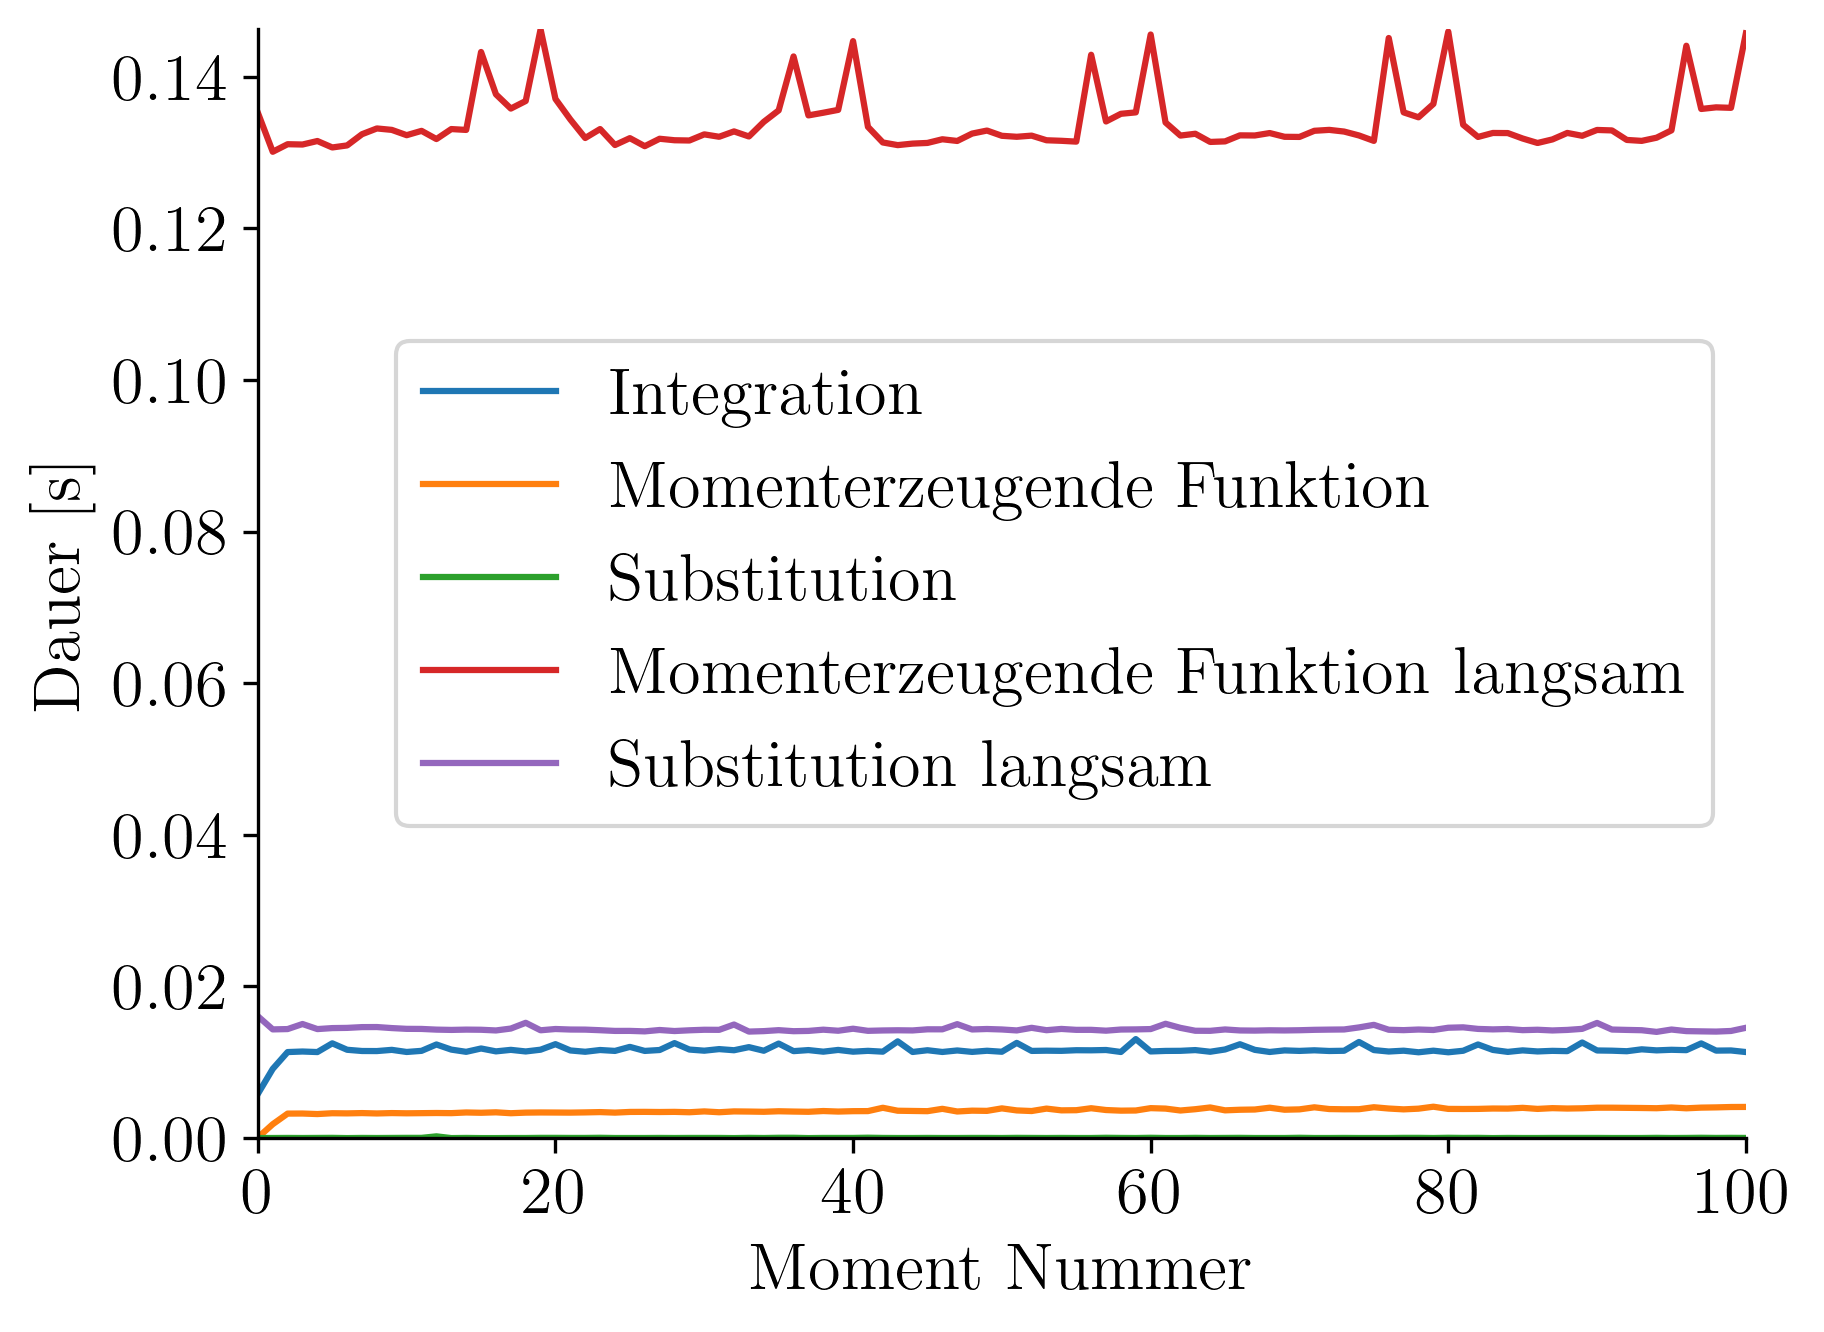
\includegraphics[width=0.5\linewidth]{./Section/Momente/Dauer Exp.png}
\vspace*{-.3\baselineskip}
\caption{Dauer der Berechnung der ersten hundert Momente einer $\Exp(\lambda)$-Verteilung}
\end{figure}

Für die Erstellung der Daten lassen wir die ersten hundert Momente hundertmal berechnen. Für Integration verwenden wir die \lstinline|_moment_integration|- und für momenterzeugende Funktion die \lstinline|_moment_generating|-Methode. Für die langsam-Kurven wird vor jeder Berechnung das \lstinline|MGF|-Attribut gelöscht. Somit muss dort jedes Mal die momenterzeugende Funktion neu berechnet werden. Für Substitution wird zu Beginn (ohne Messung der Zeit) das $n$-te Momente berechnet und anschließend für $n$ der entsprechende Wert eingesetzt. Im langsamen Fall wird das $n$-te Moment für jede Iteration von neuem berechnet.\\

Interessant sind die Spitzen bei $[15, 19]$, $[36, 40]$, $[56, 60]$ sowie $[76, 80]$ und $[96, 100]$. Dies dauert circa $10 \%$ länger, als die anderen Berechnungen. Es kann nicht am Ableiten liegen, da sonst die ähnliche Doppelspitzen auch in der Kurve für die optimierte Berechnung mit der momenterzeugenden Funktion zu finden wären. Der Garbage Collector kann mit ziemlicher Sicherheit ausgeschlossen werden, da nach jeder Berechnung der Inhalt der Variable mit \lstinline|del| gelöscht wird. Verwenden wir einen anderen Computer, so erhalten wir

\begin{figure}[H]
\centering
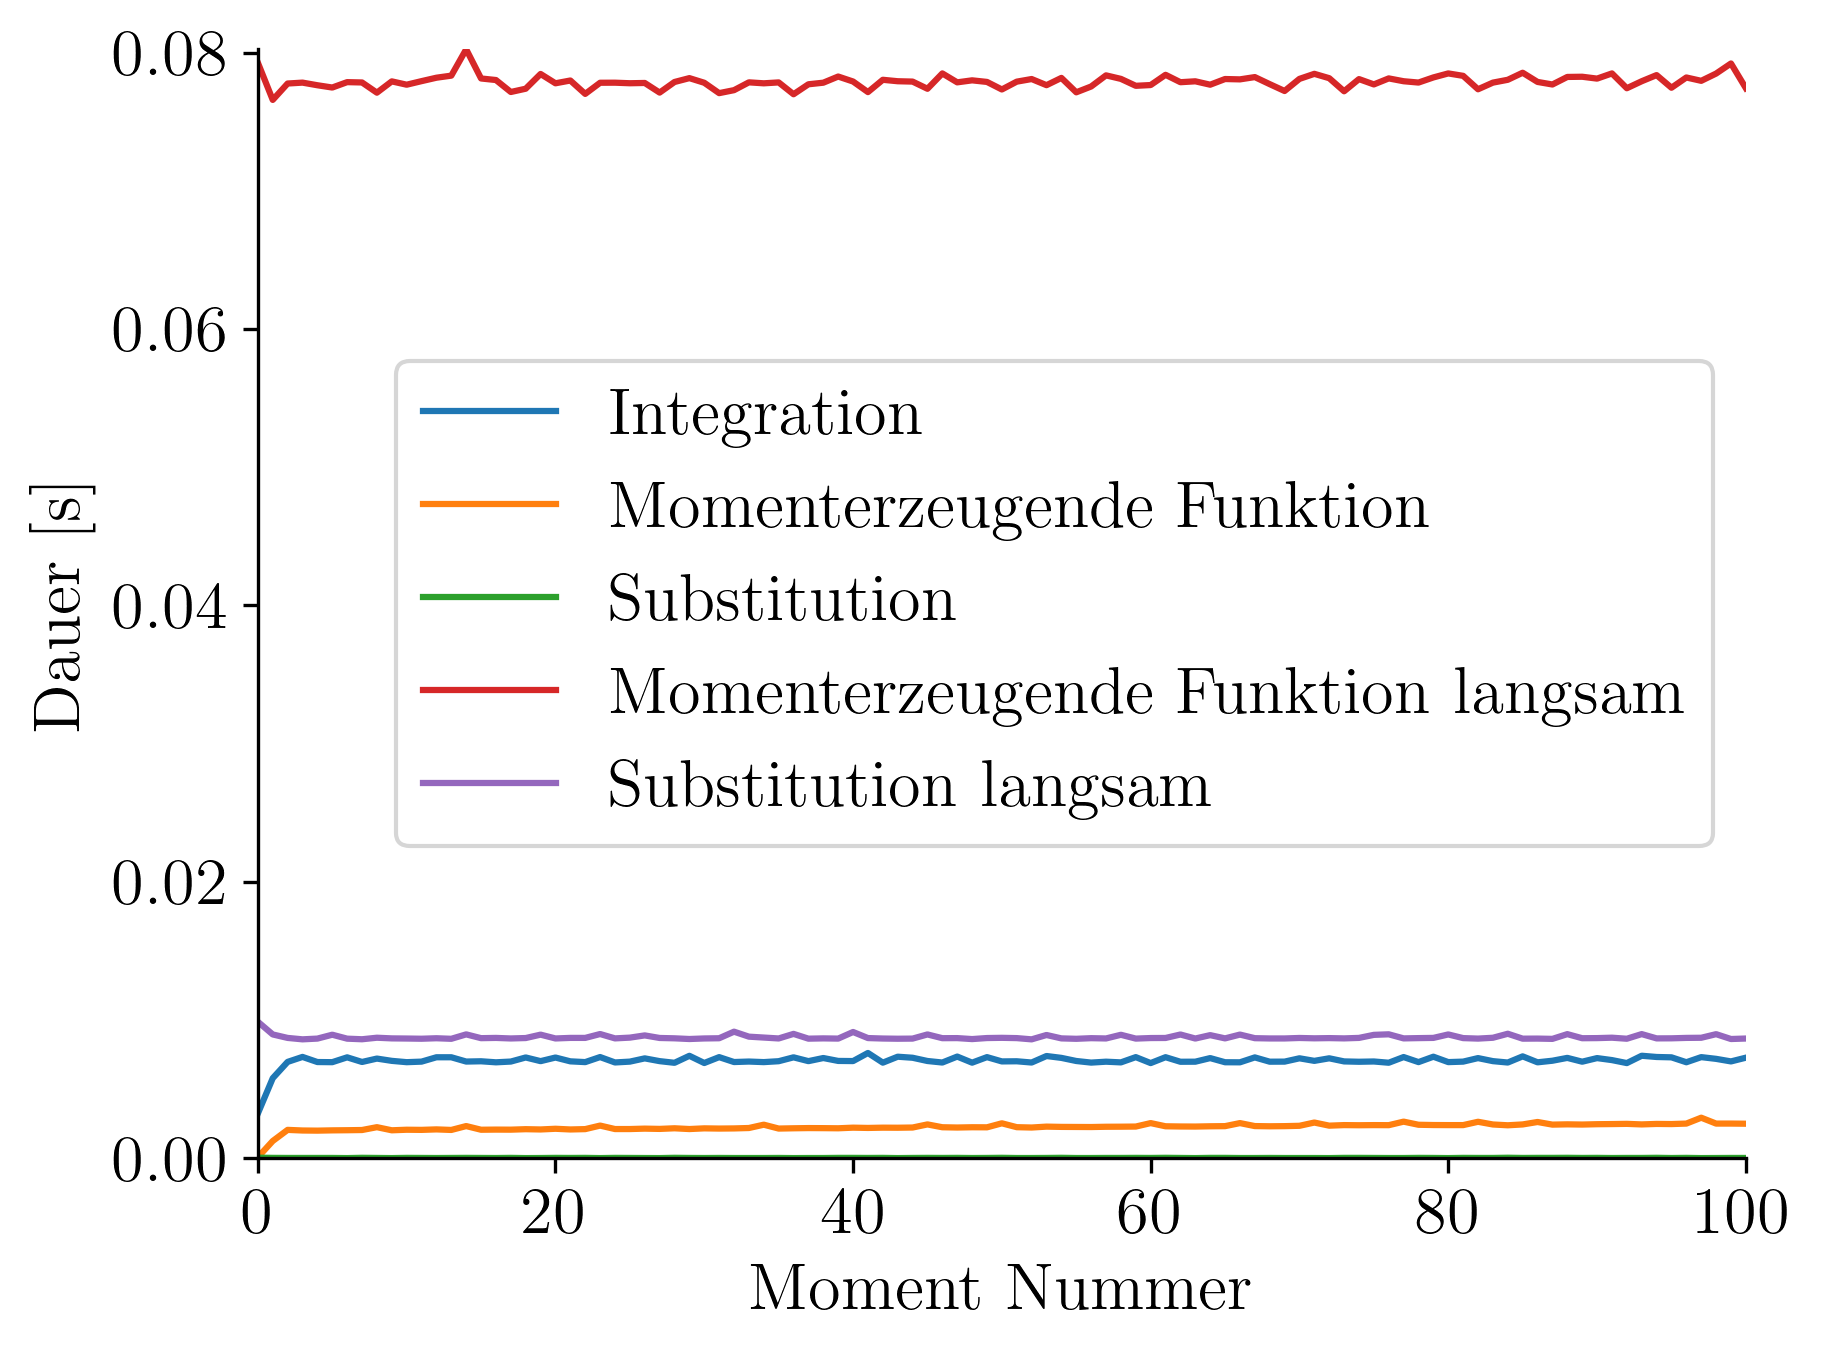
\includegraphics[width=0.5\linewidth]{./Section/Momente/Dauer Exp Alex.png}
\vspace*{-.3\baselineskip}
\caption{Dauer der Berechnung der ersten hundert Momente einer $\Exp(\lambda)$-Verteilung}
\end{figure}

An dieser Grafik lässt sich feststellen, dass das erste System um etwa die Hälfte langsamer ist als das zweite. Zudem treten die angesprochenen Spitzen nicht erneut auf. Daraus lässt sich schließen, dass diese Anomalie vermutlich nichts mit dem Programm selbst zu tun hat.\\

Für die folgende Diskussion werden wir uns mit den ersten Daten beschäftigen. Um den Graphen zu vereinfachen, ist die folgende Grafik linear interpoliert.

\begin{figure}[H]
\centering
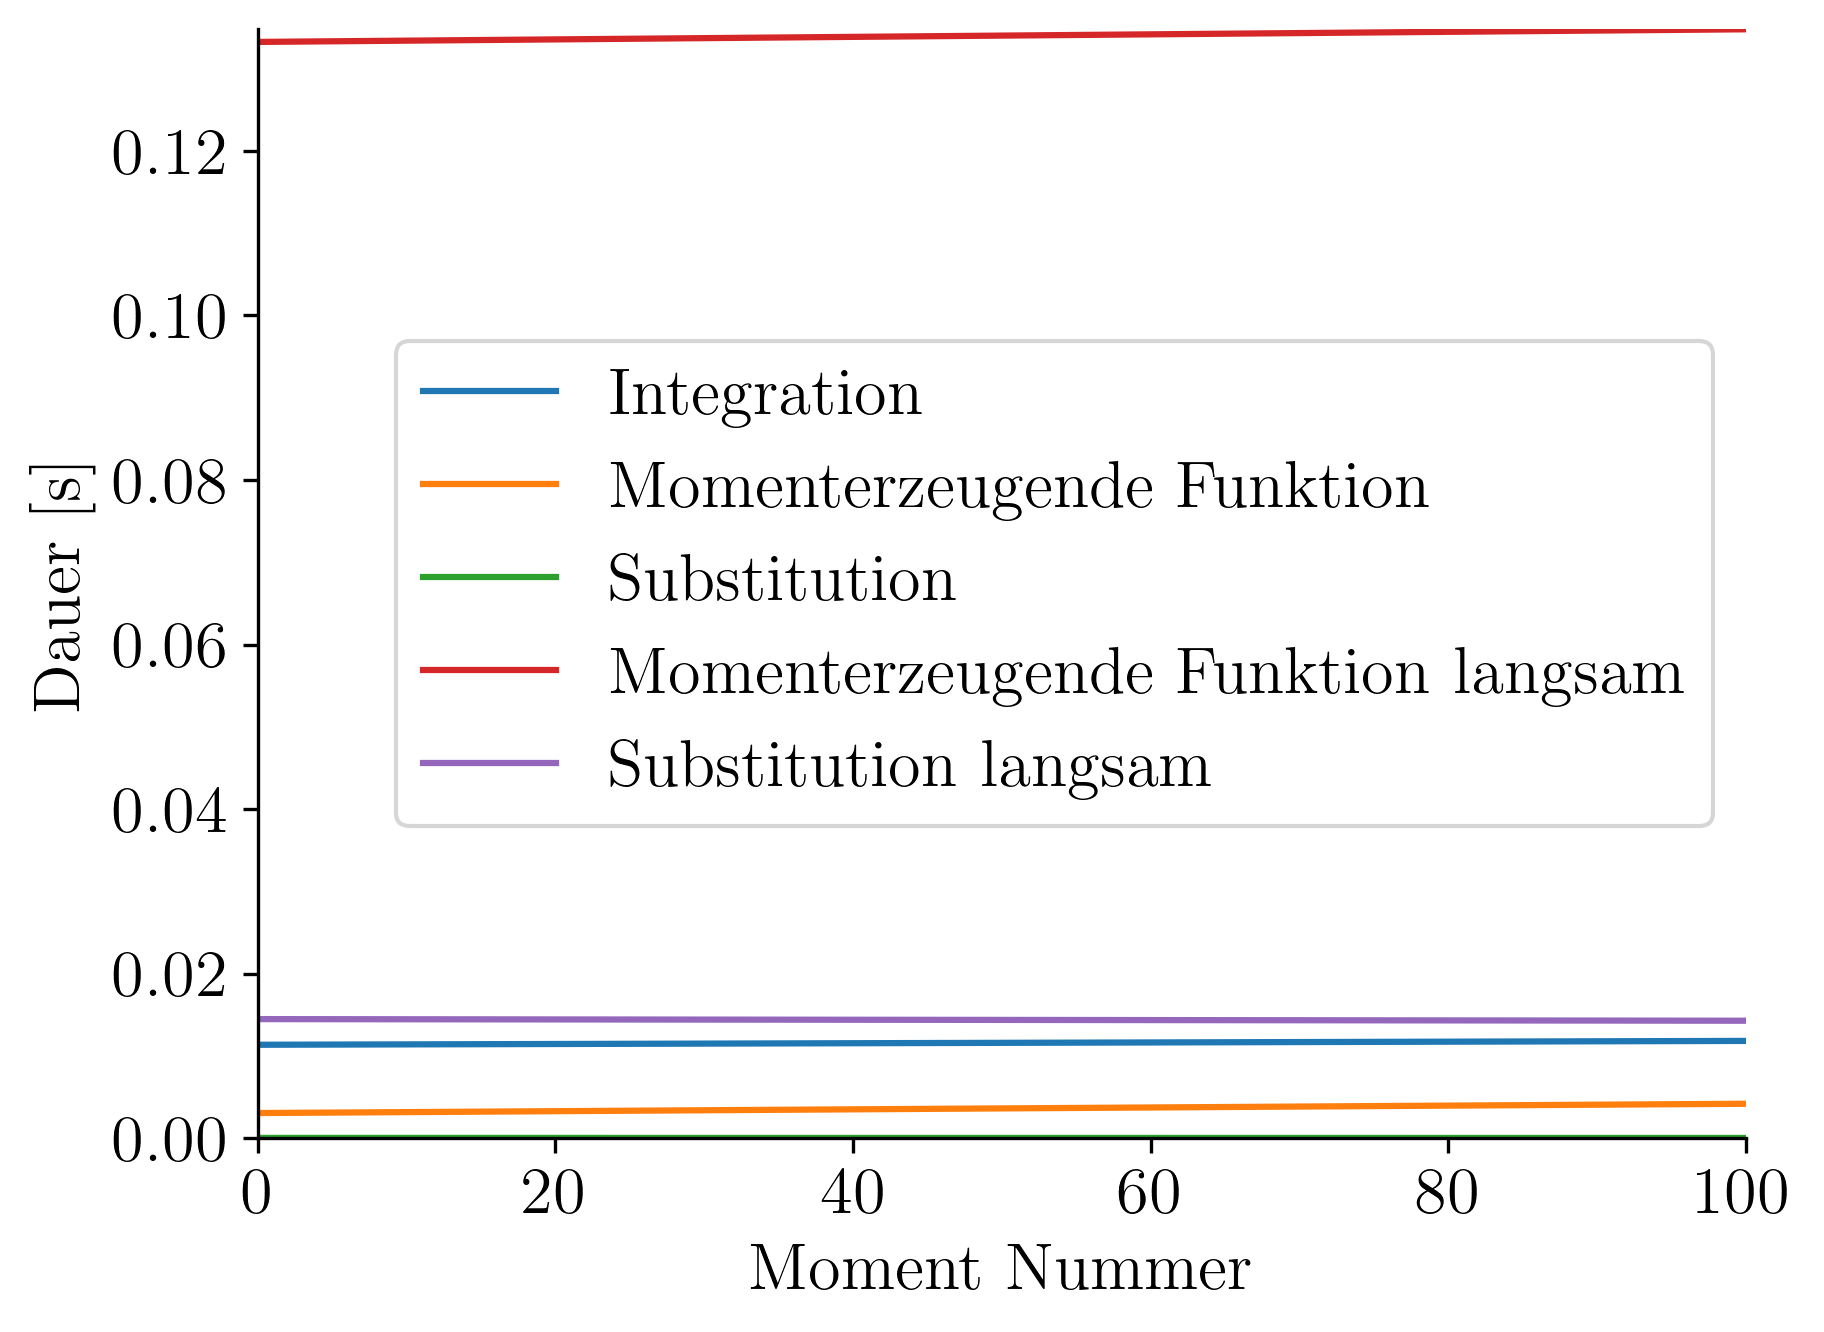
\includegraphics[width=0.5\linewidth]{./Section/Momente/Dauer Exp Lin.png}
\vspace*{-.3\baselineskip}
\caption{Interpolierte Dauer der Berechnung der ersten hundert Momente einer $\Exp(\lambda)$-Verteilung}
\end{figure}

Betrachten wir den Unterschied zwischen den beiden Geraden für die momenterzeugende Funktion, so erhalten wir eine Dauer von $0.1310$ Sekunden. Lassen wir die momenterzeugende Funktion eintausendmal berechnen, so erhalten wir im Mittel einen Wert von $0.1362$ Sekunden. Dies stimmt also mit obigem Abstand überein. Da die Berechnung der momenterzeugende Funktion scheinbar eine \glqq teure\grqq{} Berechnung ist, ist es sinnvoll die momenterzeugende Funktion, falls sie schon berechnet wurde, in dem Attribut \lstinline|MGF| zu speichern. Dies findet analog für die kumulantenerzeugende Funktion unter \lstinline|CGF| und die im folgenden Kapitel vorgestellt charakteristische Funktion unter \lstinline|CF| statt.\\

Für diese Zufallsvariable macht es scheinbar keinen großen Unterschied, mit welcher Methode man die Momente berechnet. Es ist allerdings sehr interessant, dass die Berechnung der Momente mittels Substitution, falls zuvor das $n$-te Moment berechnet quasi instantan stattfindet. Man könnte sich an dieser Stelle wundern, wieso es keine Methode gibt, die ein Moment mittels Substitution berechnet. Die Berechnung des $n$-ten Moments ist für die meisten Verteilungen höchst aufwendig und für viele Verteilungen kann SymPy auch keinen geschlossenen Ausdruck angeben. Des Weiteren haben wir, wie bei dem \hyperlink{Bsp:Nicht-Int}{\blue{Beispiel zur nicht-integrierbaren Familie}} gesehen, auch ein Problem, falls das $n$-te Moment eine stückweise Funktion ist. Es fällt auf, dass die Berechnung mithilfe der momenterzeugenden Funktion um circa $0.008$ Sekunden schneller ist, als die Berechnung mittels Integration. Daher scheint es momentan eher unsinnvoll zu sein die Integration als Standardmethode gewählt zu haben. Weiter fällt auf, dass alle Methoden nahezu konstanten Aufwand haben. Die Steigung ist jeweils im Bereich von $10^{-6}$, was vermutlich auf Messungenauigkeiten zurückzuführen ist.
\end{Beispiel}

\vspace*{-\medskipamount}

\newpage

\begin{Beispiel}{(Laufzeit Normalverteilung)}
Sei $X \sim \Nor(\mu, \sigma)$ mit $\mu, \sigma > 0$ normalverteilt. Da die Berechnungen hier deutlich mehr Zeit in Anspruch nehmen, lassen wir die ersten hundert Momente nur zehnmal berechnen und  verzichten auf die unoptimierten Varianten der Berechnungen.

\begin{figure}[H]
\centering
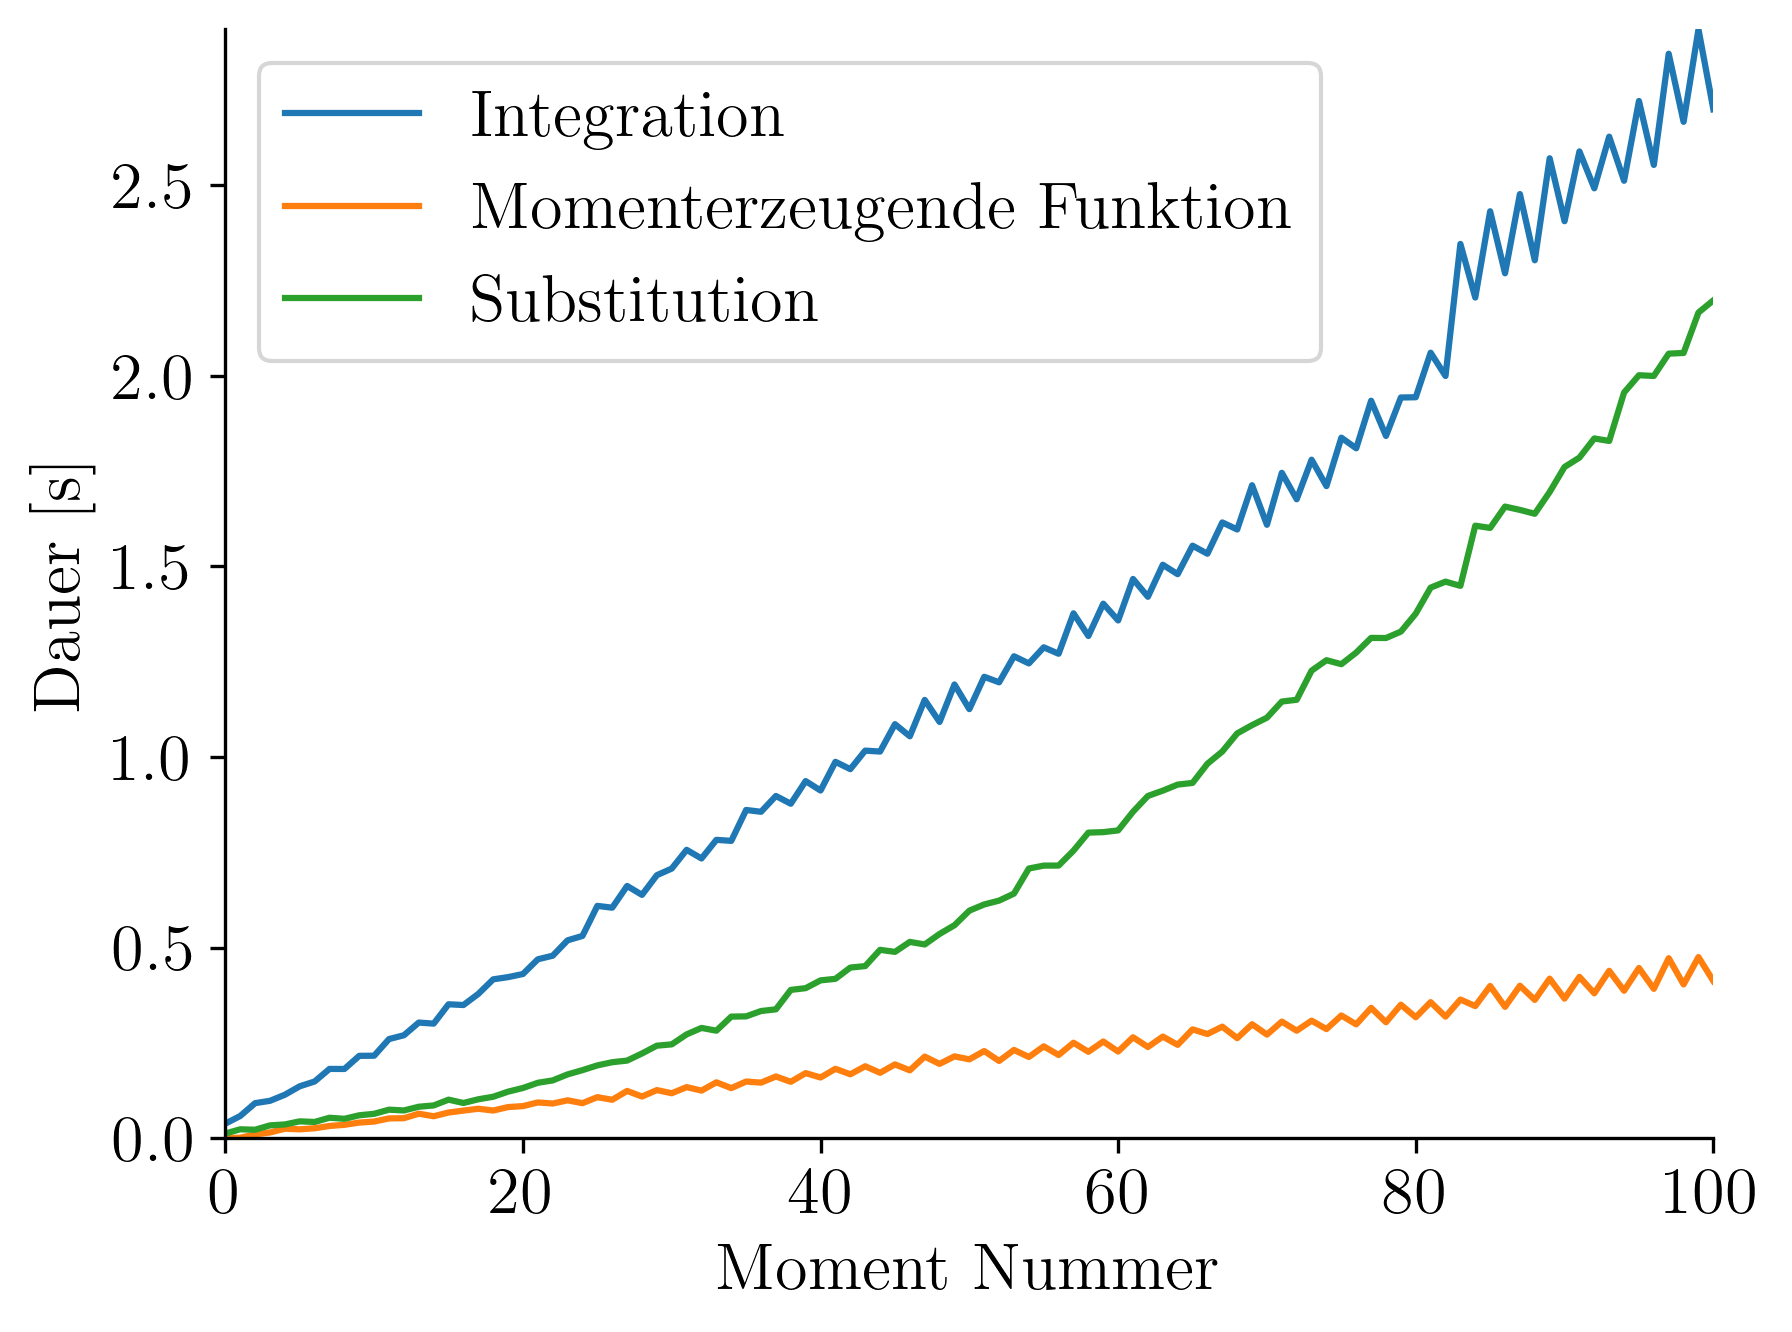
\includegraphics[width=0.5\linewidth]{./Section/Momente/Dauer Nor Falsch.png}
\vspace*{-.3\baselineskip}
\caption{Dauer der Berechnung der ersten hundert Momente einer $\Nor(\mu, \sigma)$-Verteilung ohne Vereinfachung}
\end{figure}

Dieser Plot spiegelt aber nicht ganz die Wahrheit wieder. Lassen wir mit SymPy das $n$-te Moment berechnen, so erhalten wir
\[\mathbb{E}(X^n) = \frac{2^{\frac{n}{2} - 1} \sigma^{n} \left(\left(-1\right)^{n} {G_{1, 2}^{2, 1}\left(\begin{matrix} \frac{1}{2} - \frac{n}{2} &  \\0, \frac{1}{2} &  \end{matrix} \middle| {\frac{\mu^{2}}{2 \sigma^{2}}} \right)} + {G_{1, 2}^{2, 1}\left(\begin{matrix} \frac{1}{2} - \frac{n}{2} &  \\0, \frac{1}{2} &  \end{matrix} \middle| {\frac{\mu^{2} e^{2 i \pi}}{2 \sigma^{2}}} \right)}\right) e^{- \frac{\mu^{2}}{2 \sigma^{2}}}}{\pi}~.\]
Setzen wir beispielsweise den Wert $n = 6$ ein, so erhalten wir
\[\mathbb{E}(X^6) = \frac{2 \sigma^{4} \left({G_{1, 2}^{2, 1}\left(\begin{matrix} - \frac{3}{2} &  \\0, \frac{1}{2} &  \end{matrix} \middle| {\frac{\mu^{2}}{2 \sigma^{2}}} \right)} + {G_{1, 2}^{2, 1}\left(\begin{matrix} - \frac{3}{2} &  \\0, \frac{1}{2} &  \end{matrix} \middle| {\frac{\mu^{2} e^{2 i \pi}}{2 \sigma^{2}}} \right)}\right) e^{- \frac{\mu^{2}}{2 \sigma^{2}}}}{\pi}~.\]
Wir wollen eigentlich den Ausdruck
\[\mathbb{E}(X^6) = \mu^6 + 15 \mu^4 \sigma^2 + 45 \mu^2 \sigma^4 + 15 \sigma^6~.\]
Diesen erhalten wir durch die Anwendung von \lstinline|simplify| auf obigen Ausdruck. Verwenden wir diesen Schritt auch in der obigen Berechnung, so erhalten wir das folgende Bild.

\begin{figure}[H]
\centering
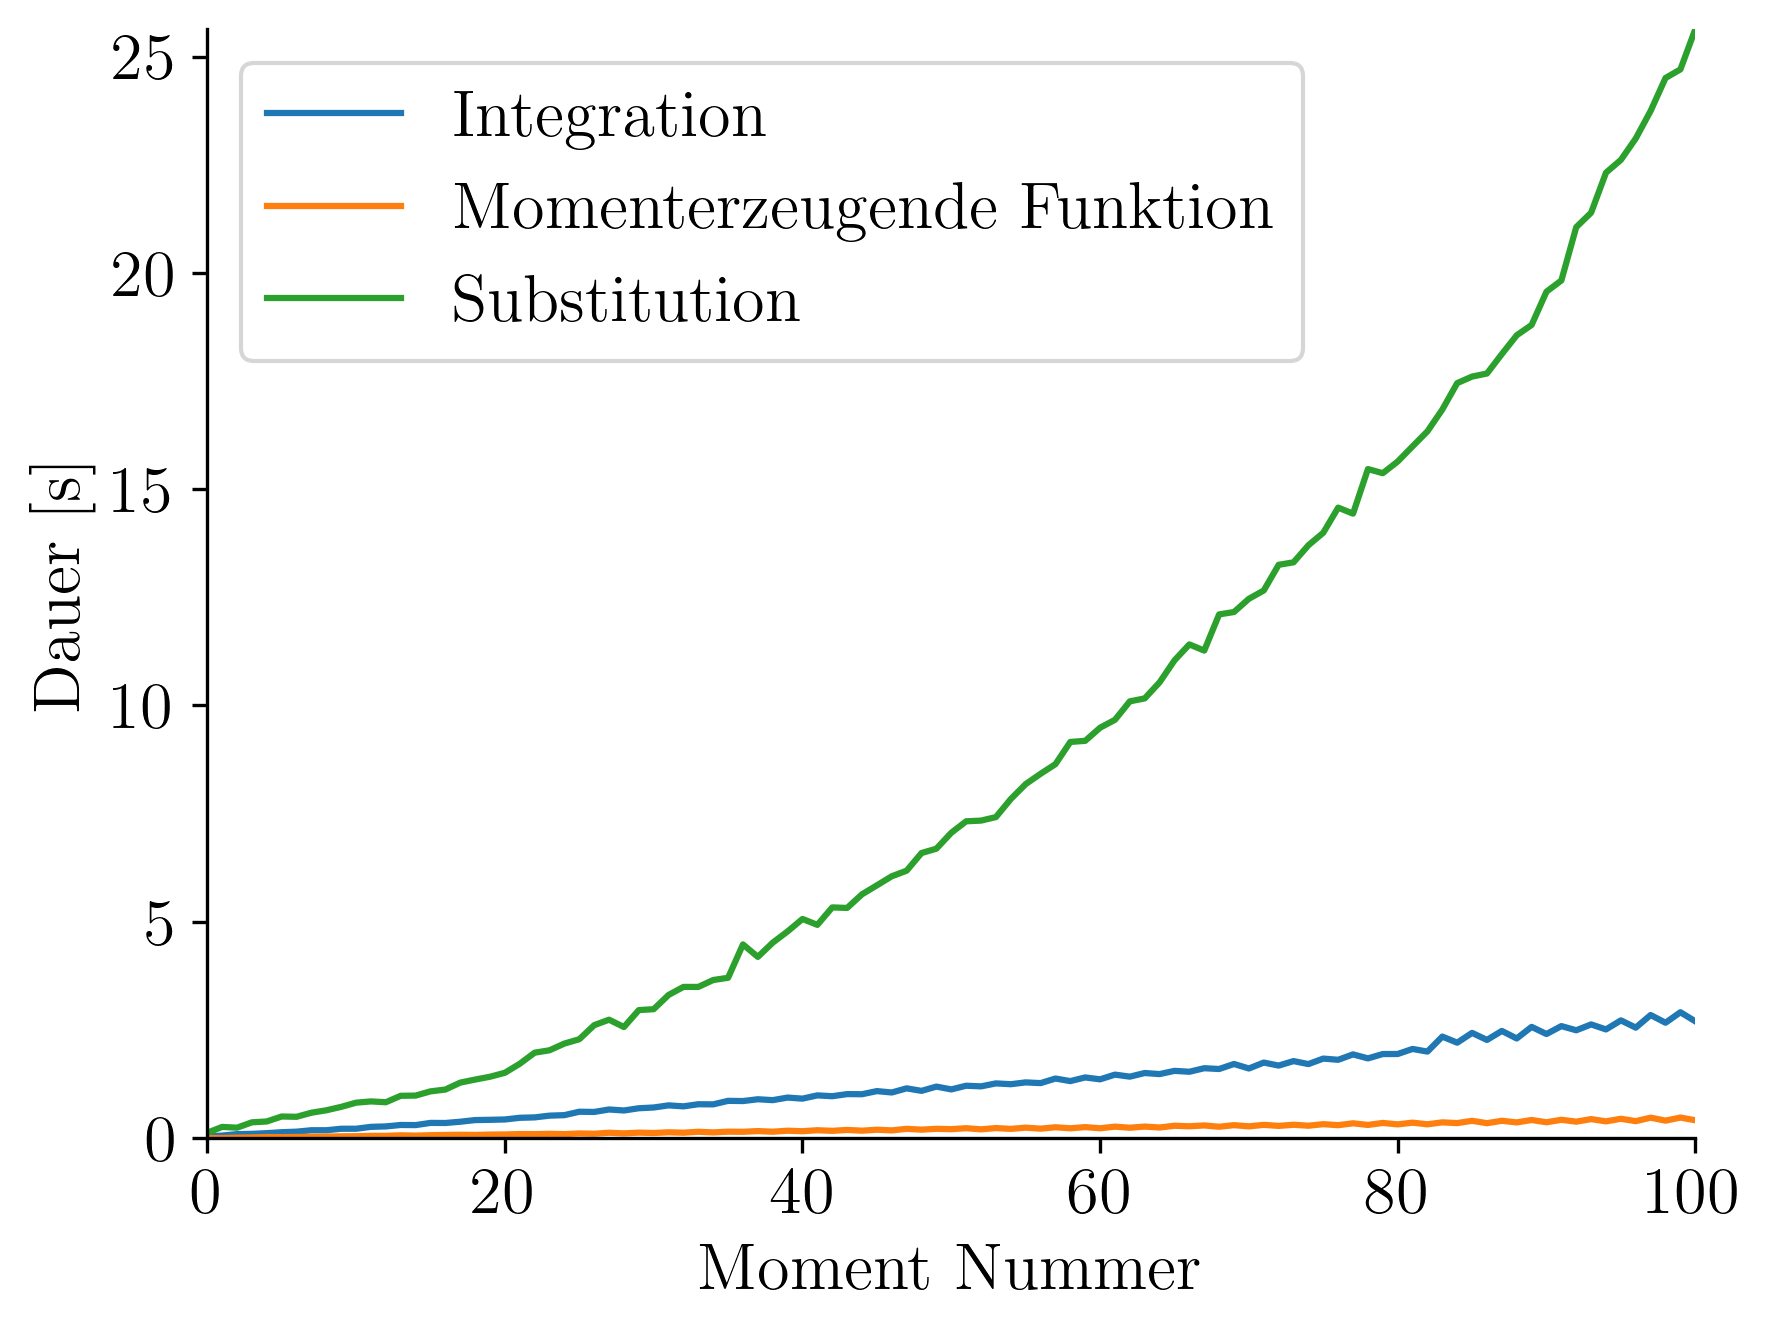
\includegraphics[width=0.5\linewidth]{./Section/Momente/Dauer Nor.png}
\vspace*{-.3\baselineskip}
\caption{Dauer der Berechnung der ersten hundert Momente einer $\Nor(\mu, \sigma)$-Verteilung mit Vereinfachung}
\end{figure}

Wir erkennen, dass Substitution für eine Normalverteilung aufgrund der nötigen, scheinbar sehr kostspieligen Vereinfachung ein grauenhaft ineffizientes Verfahren ist. Bei der Exponentialverteilung haben wir diese Vereinfachung nicht benötigt, da SymPy selbst große Fakultäten sofort berechnen kann. Wir erkennen weiter, dass der Aufwand zur Berechnung der Moment nicht mehr konstant. Für die Substitution scheint er quadratisch zu sein und für die anderen Methoden linear. Interessant ist auch, dass die Berechnung mittels der momenterzeugenden Funktion deutlich schneller abläuft als die Berechnung mittels Integration. Verwenden wir eine lineare Interpolation, so erhalten wir eine Steigung von $0.004$ beziehungsweise $0.240$.
\end{Beispiel}

Wir werden nun als Beispiel einer der einfachsten stetigen Verteilungen betrachten.

\begin{Beispiel}{(Laufzeit stetige Gleichverteilung)}
Sei $X$ auf $[a, b]$ gleichverteilt mit $a < b$ aus $\mathbb{R}$. Lassen wir an dieser Stelle die ersten hundert Moment fünfzigmal mit den drei Methoden berechnen, so erhalten wir den folgenden Plot.

\begin{figure}[H]
\centering
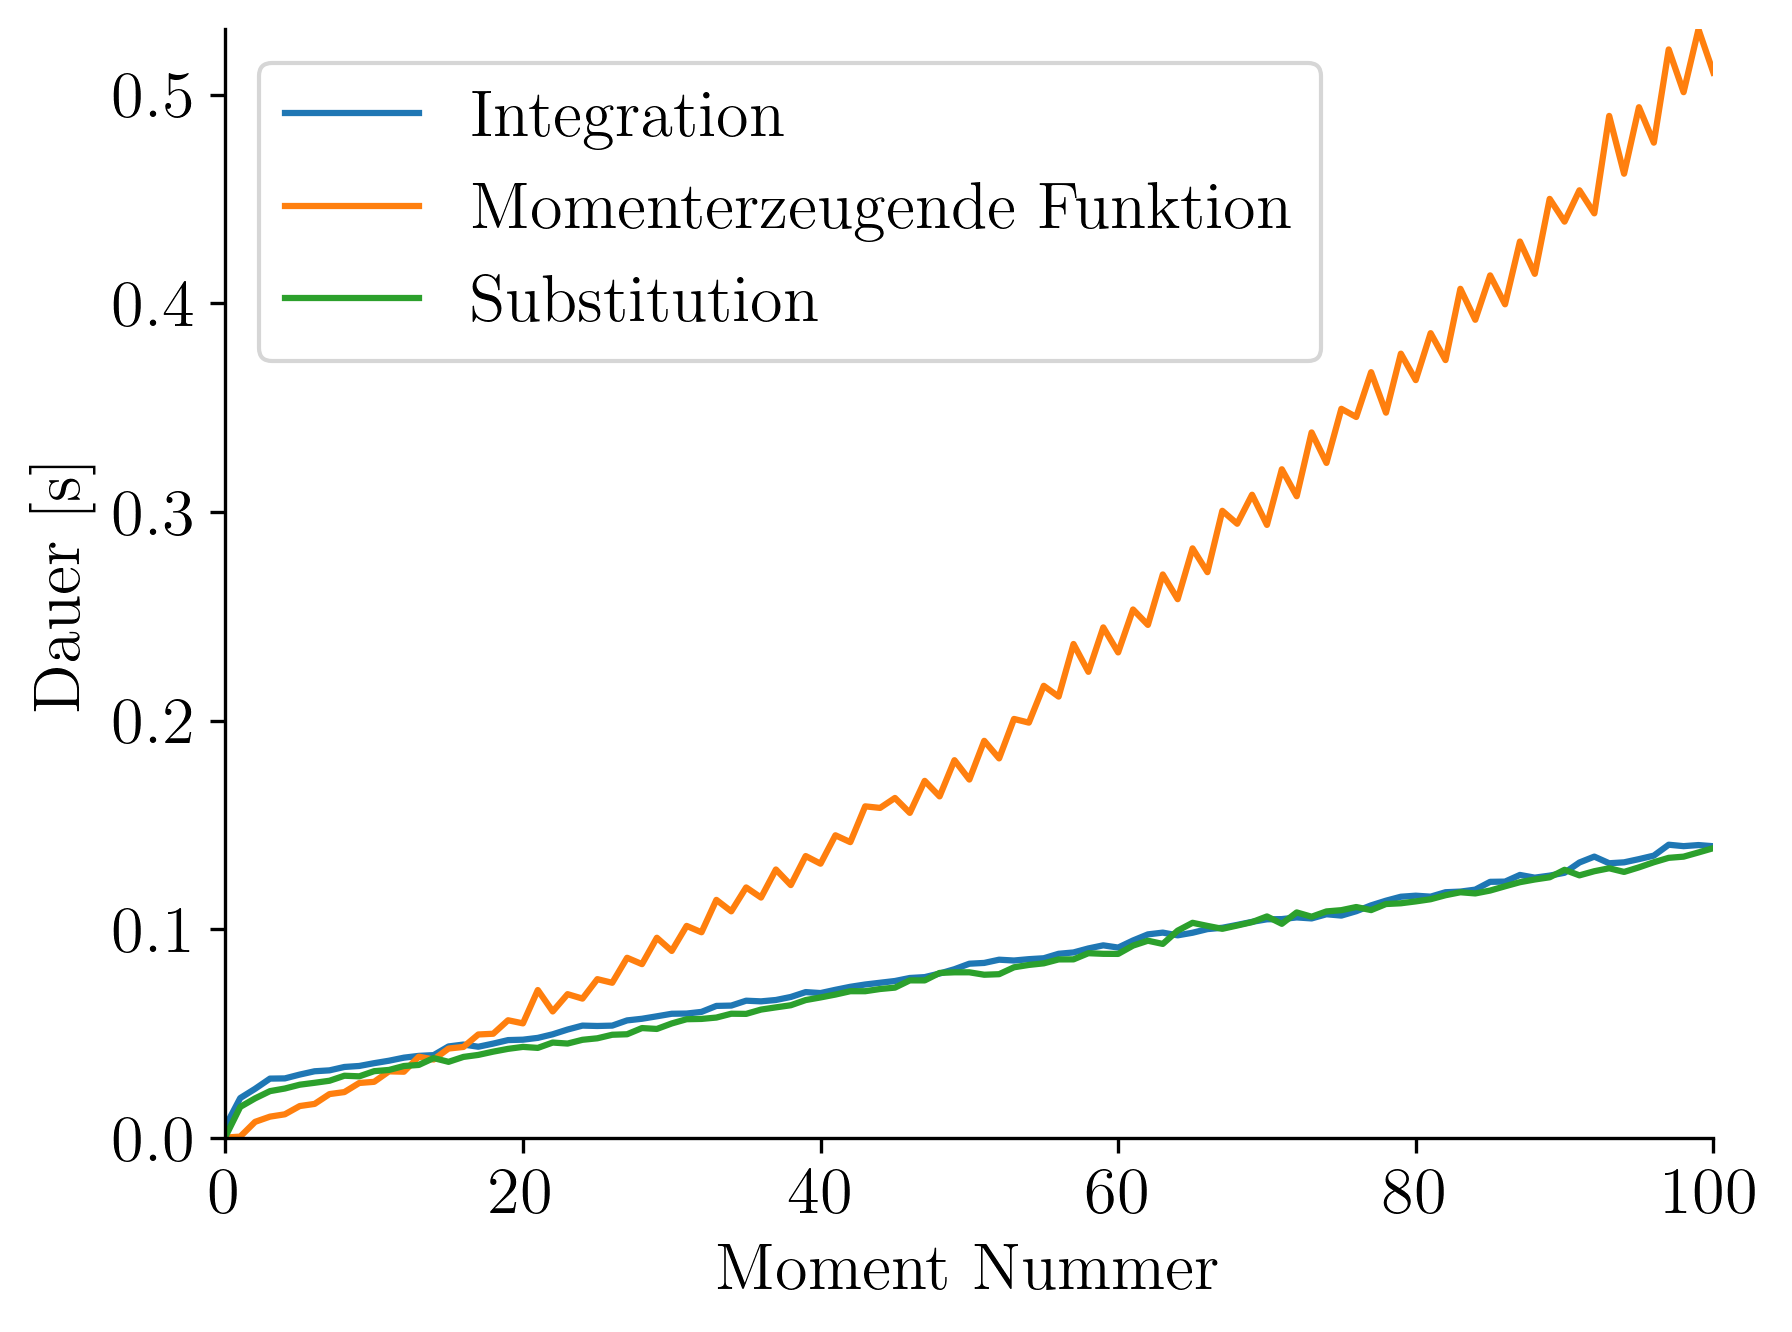
\includegraphics[width=0.5\linewidth]{./Section/Momente/Dauer Gleich.png}
\vspace*{-.3\baselineskip}
\caption{Dauer der Berechnung der ersten hundert Momente einer Gleichverteilung auf $[a, b]$}
\end{figure}

Wir erkennen nun etwas scheinbar Überraschendes. Die Berechnung mittels der momenterzeugenden Funktion ist langsamer. Die Berechnung mittels Integration und Substitution scheinen wieder lineares Wachstum zu haben und sind interessanterweise gleich schnell. Die Berechnung mit der momenterzeugenden Funktion scheint quadratischen Aufwand zu haben.
\end{Beispiel}

Nun werden wir uns ein finites Beispiel anschauen.

\begin{Beispiel}{(Laufzeit Bernoulli-Verteilung)}
Sei $X \sim \Ber(p)$ mit $p \in (0, 1)$ Bernoulli-verteilt. Lassen wir die ersten hundert Momente tausendmal berechnen, so erhalten wir die folgende Grafik.

\begin{figure}[H]
\centering
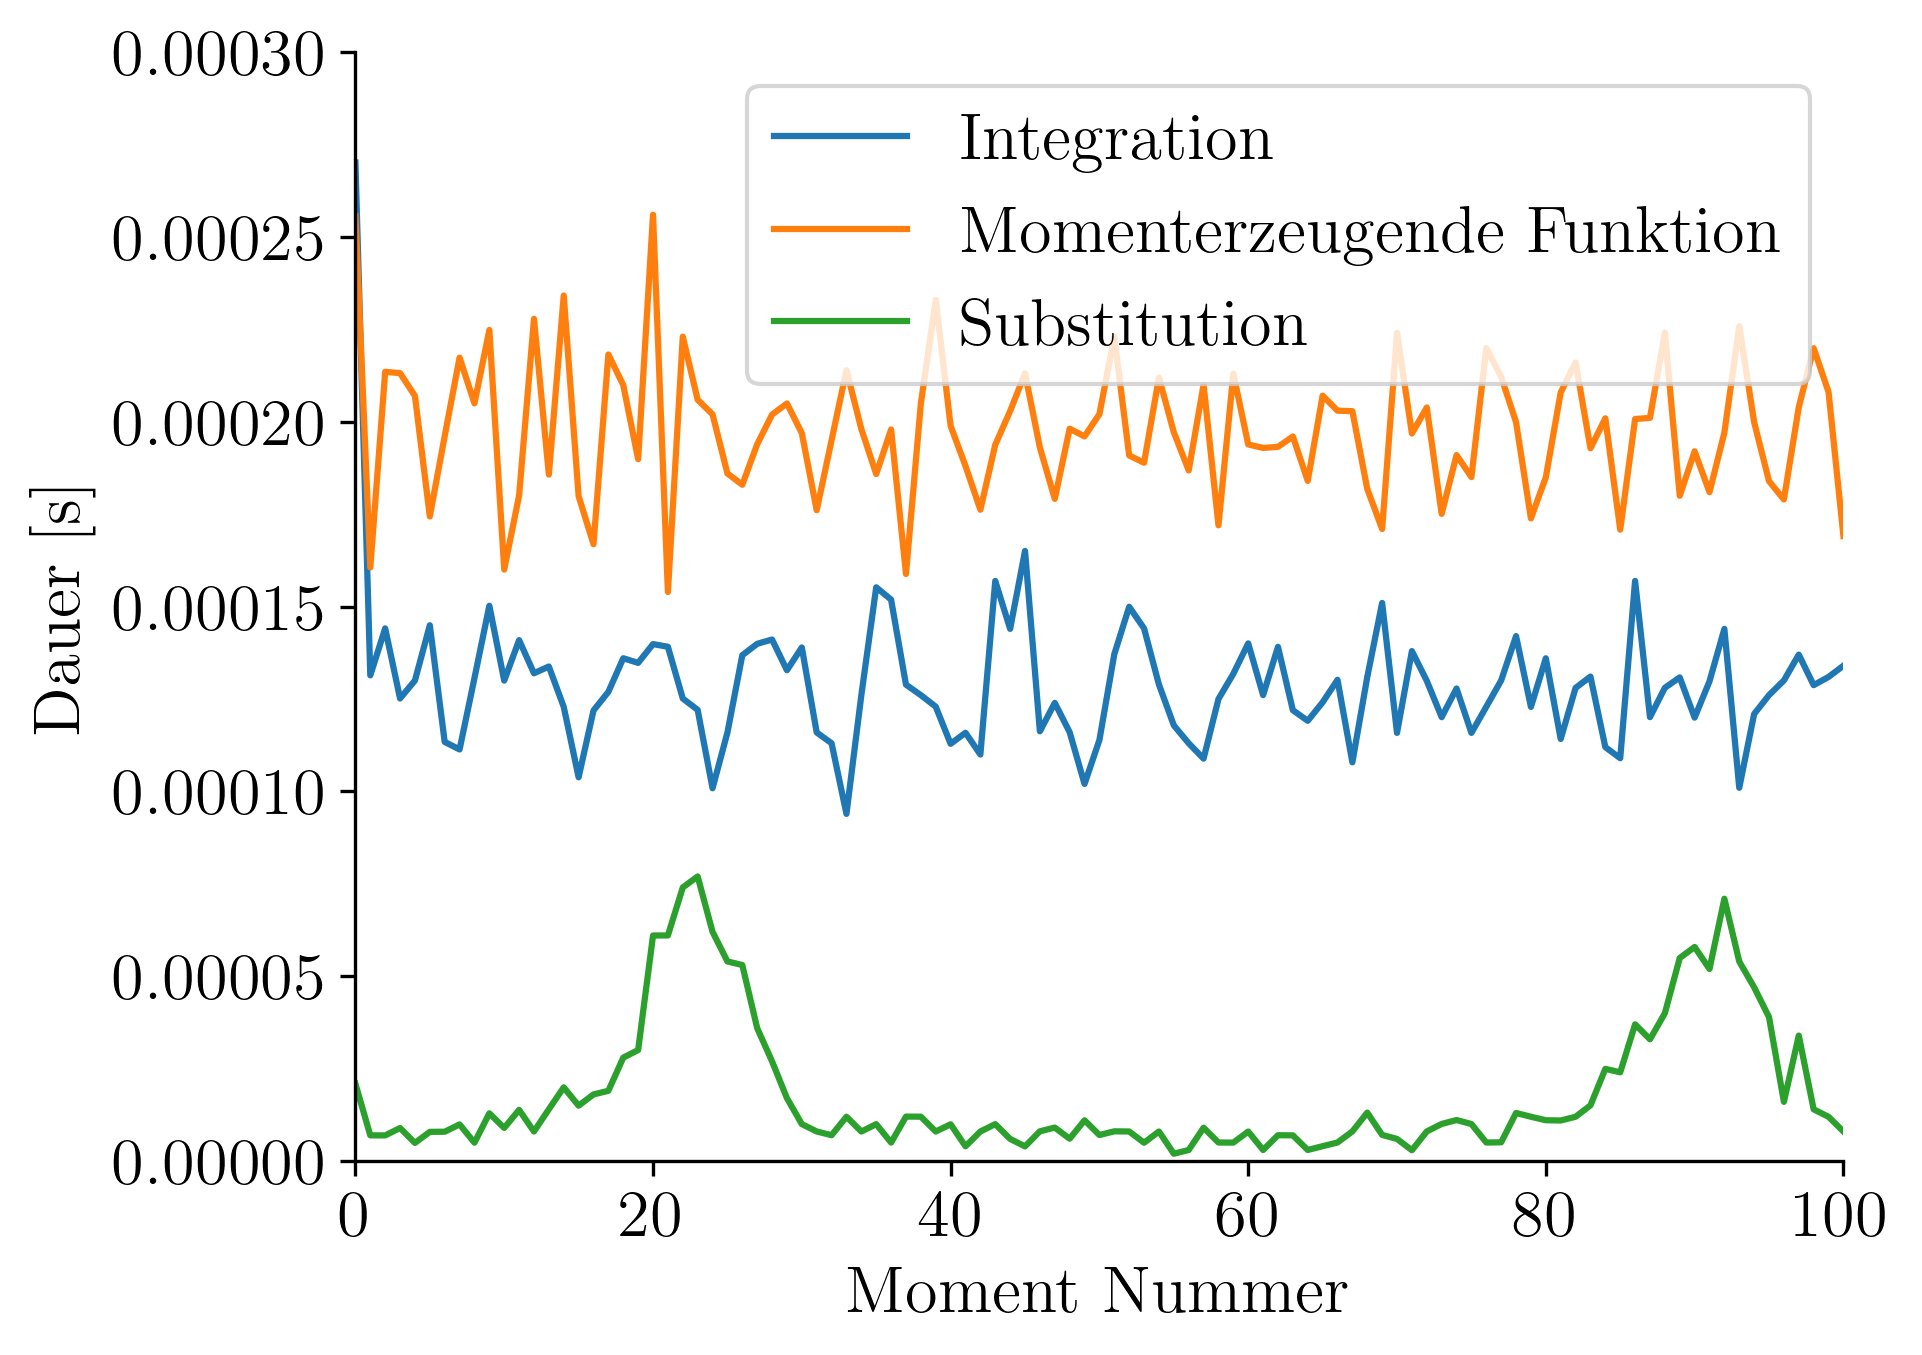
\includegraphics[width=0.5\linewidth]{./Section/Momente/Dauer Ber.png}
\vspace*{-.3\baselineskip}
\caption{Dauer der Berechnung der ersten hundert Momente einer $\Ber(p)$-Verteilung}
\end{figure}

Dieses Beispiel ist eher zum Spaß gedacht. Wir sehen, dass die Dauer der Berechnung im Zehntel Millisekundenbereich liegt. Diese unglaubliche Geschwindigkeit lässt sich darauf zurückführen, dass hier nur simpelste Berechnungen durchgeführt werden müssen. Es muss null oder eins potenziert werden und anschließend mit $1 - p$ respektive $p$ multipliziert werden. Aufgrund dieser Geschwindigkeit sind die Daten auch so rauschend, da die gesamte Berechnung nur wenige Sekunden gedauert hat und somit kleinste Nebentätigkeiten des Betriebssystem große Schwankungen hervorrufen. Vermutlich ist die Berechnung der Momente aller finiten Verteilungen derart \glqq einfach\grqq{}, da hier wie gesagt nur die Grundoperationen benötigt werden und diese sehr gut optimiert sind.
\end{Beispiel}

Als letztes Beispiel werden wir eine diskrete Zufallsvariable betrachten.

\begin{Beispiel}{(Laufzeit Poisson-Verteilung)}
Sei $X \sim \Poiss(\lambda)$ mit $\lambda > 0$ Poisson-verteilt. Hier lassen wir nur die ersten zwanzig Moment zehnmal berechnen. Wir erhalten den folgenden Plot.

\begin{figure}[H]
\centering
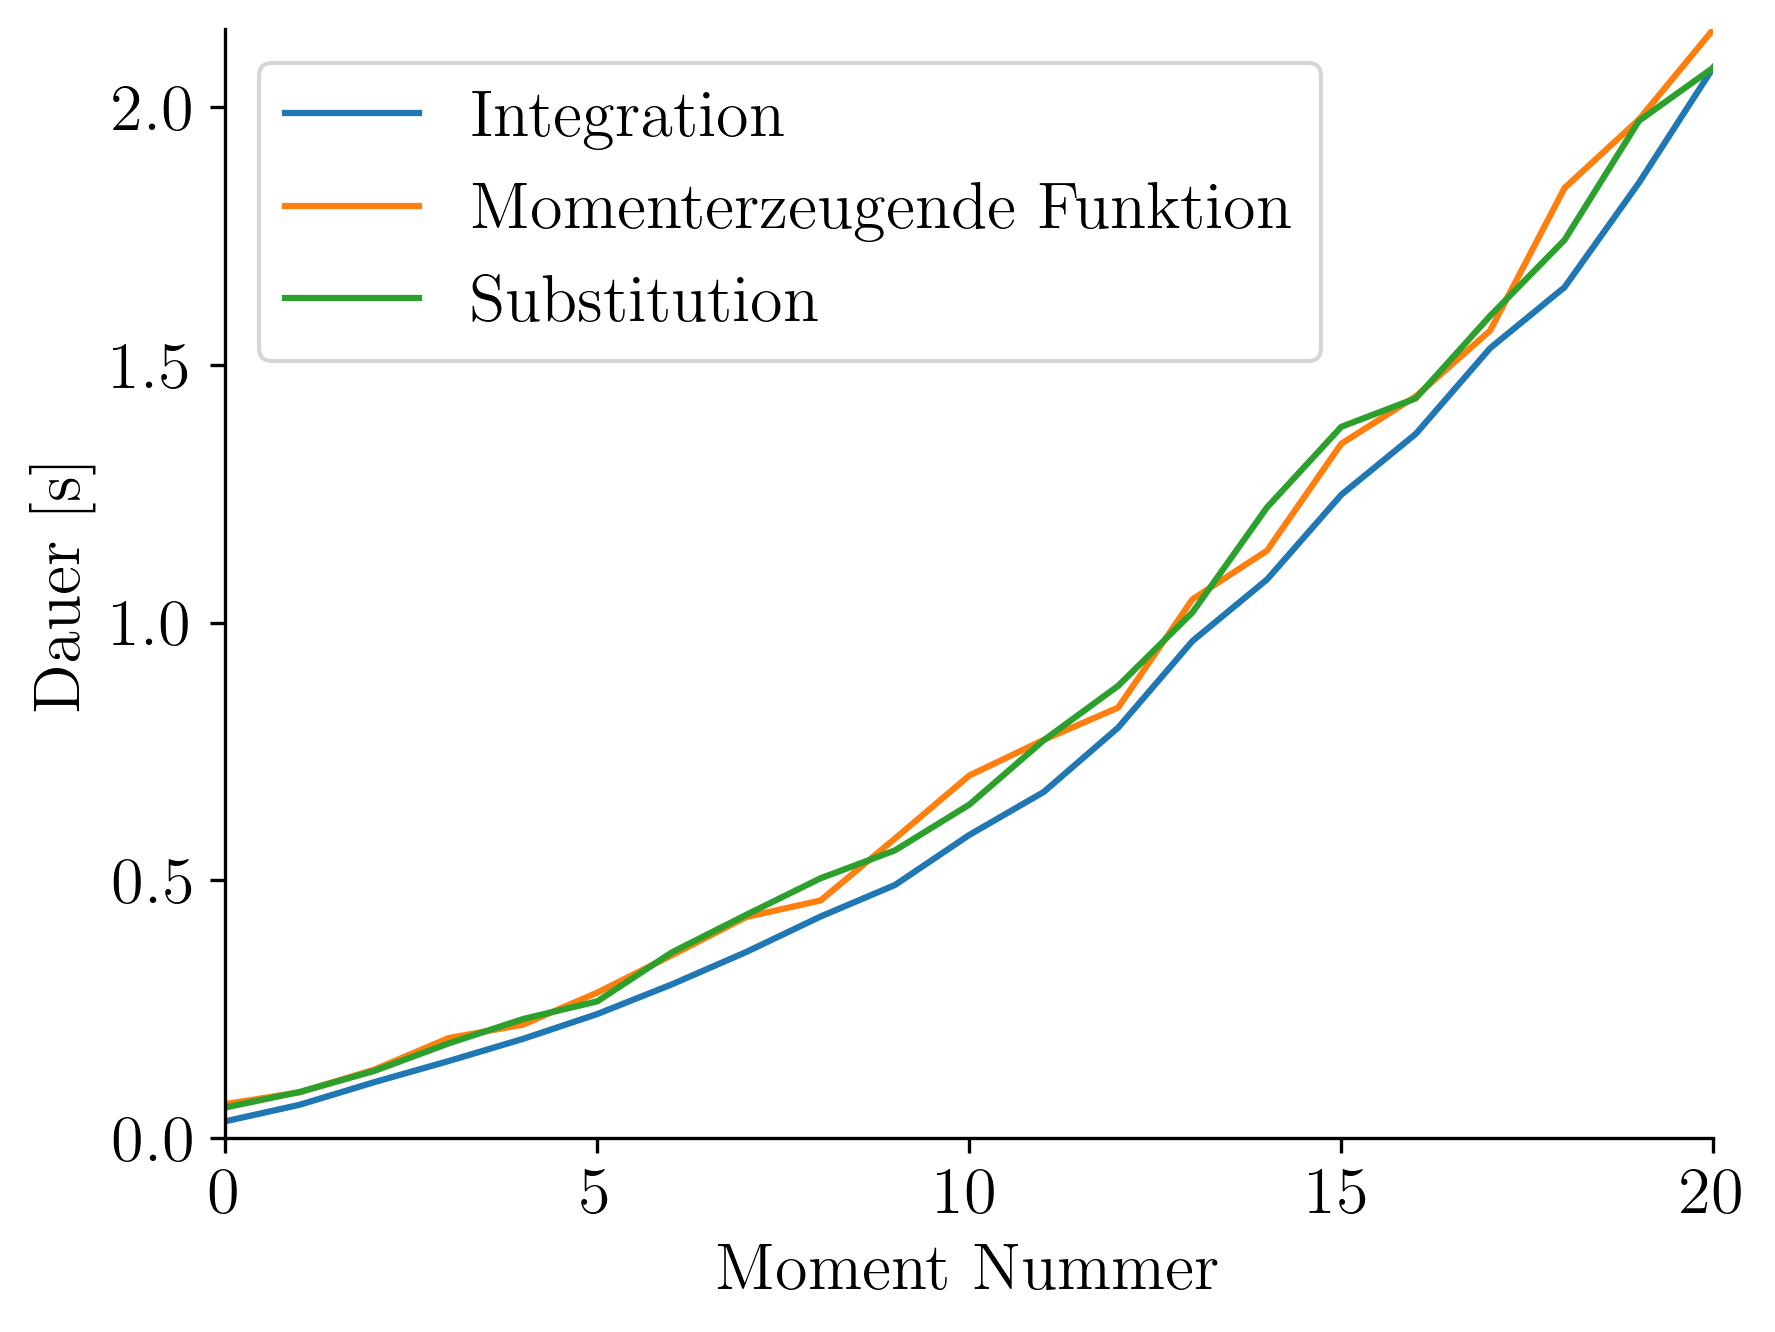
\includegraphics[width=0.5\linewidth]{./Section/Momente/Dauer Poisson.png}
\vspace*{-.3\baselineskip}
\caption{Dauer der Berechnung der ersten zwanzig Momente einer $\Poiss(\lambda)$-Verteilung}
\end{figure}

Interessanterweise sind hier alle drei Arten der Berechnung ziemlich genau gleich schnell und zeigen mindestens quadratisches Wachstum. Vermutlich sind alle Berechnungen ungefähr gleich schnell, da SymPy für Summen beziehungsweise Reihen keine so starken Werkzeuge hat, wie für Integrale. Dies ist vermutlich auch der Grund, wieso schon das zwanzigste Moment über $2$ Sekunden Rechenzeit benötigt.
\end{Beispiel}

Man stellt sich jetzt natürlich die Frage, was wir aus all diesen Beispielen gelernt haben. Es ist leider nicht klar, welche der Methoden \glqq die Beste\grqq{} ist. Je nach Verteilung ist eine andere Methode am schnellsten. Außerdem haben wir gelernt, dass finite Verteilungen blitzschnell berechenbar sind und diskrete Verteilungen scheinbar größere Probleme machen, wobei dies noch etwas näher beleuchtet werden sollte. Bei stetigen Verteilungen ist von der Rechendauer alles dabei.


\subsection{Charakteristische Funktionen}

In diesem Abschnitt wollen wir uns mit einer weiteren Funktion beschäftigen, die sehr eng mit der momenterzeugenden Funktion verwandt ist.

\begin{Definition}{(Charakteristische Funktion)}
Sei $(\Omega, \mathscr{A}, \mathbb{P})$ ein Wahrscheinlichkeitsraum und $X$ eine reelle Zufallsvariable. Die \textit{charakteristische Funktion von $X$} \en{characteristic function} ist definiert durch
\[C_X(t) := \mathbb{E}\left( \exp(i t X) \right)~.\]
Insbesondere ist $C_X: \mathbb{D} \rightarrow \mathbb{C}: t \mapsto C_X(t)$ für $\mathbb{D} := \{ t \in \mathbb{R} \mid C_X(t) < \infty\}$ eine komplexwertige Abbildung.
\end{Definition}

Mit dem folgenden Satz werden wir einen einfachen Zusammenhang zwischen momenterzeugender und charakteristischer Funktion erkennen.

\begin{Satz}{(Zusammenhang charakteristische und momenterzeugende Funktion)}
Sei $(\Omega, \mathscr{A}, \mathbb{P})$ ein Wahrscheinlichkeitsraum und $X$ eine reelle Zufallsvariable mit momenterzeugender Funktion $M_X$. Es gilt für $t \in \mathbb{D}$
\[M_X(i t) = C_X(t)~.\]
\end{Satz}

\begin{Beweis}{}
Betrachte zu $t \in \mathbb{D}$
\begin{align*}
M_X\left( i t \right) &= \mathbb{E}\left( \exp(i t X) \right)\\
&= C_X(t)~.
\end{align*}
Wir können an dieser Stelle wieder einen \glqq Beweis\grqq{} mit SymPy führen. Wir formen die zu beweisende Identität um und erhalten
\[0 = M_X(i t) - C_X(t)~.\]
Wir betrachten nun.
\begin{lstlisting}[numbers=left, numberstyle=\tiny\color{codegray}]
x = sym.Symbol('x', real=True)
t = sym.Symbol('t', real=True)
f = sym.Function('f')(x)
rv = RandomVariableContinuous(f, x, force_density=True)
moment_generating_function = rv.moment_generating_function()
characteristic_function = rv.characteristic_function()
solution = moment_generating_function.subs(t, sym.I * t) - characteristic_function
\end{lstlisting}
Mit dem Ergebnis von \lstinline|0|, was zu zeigen war.
\end{Beweis}

\medskip

Wir können nun auch die charakteristische Funktion verwenden, um Momente zu bestimmen.

\begin{Satz}{(Momente mit charakteristischer Funktion)}
Sei $(\Omega, \mathscr{A}, \mathbb{P})$ ein Wahrscheinlichkeitsraum und $X$ eine reelle Zufallsvariable. Existiert das $n$-te Momente, so gilt
\[\mathbb{E}(X^n) = \left[\frac{\d^n}{\d t^n} \frac{C_X(t)}{i^n}\right]_{t = 0}~.\]
\end{Satz}

\begin{Beweis}{}
Betrachte mit vorigem Satz
\begin{align*}
\left[\frac{\d^n}{\d t^n} \frac{C_X(t)}{i^n}\right]_{t = 0} &= \left[\frac{\d^n}{\d t^n} \frac{M_X\left( i t \right)}{i^n}\right]_{t = 0}~.
\intertext{Nach der Kettenregel erhalten wir durch das Ableiten einen Faktor von $i^n$. Da wir $t = 0$ einsetzen, ist die Multiplikation mit $i$ in der momenterzeugenden Funktion irrelevant und wir erhalten aus dem \hyperlink{Kor:Momente_MomGenFun}{\blue{Korollar über die Berechnung der Momente mithilfe der momenterzeugenden Funtion}}}
&= \frac{i^n}{i^n} \mathbb{E}(X^n)\\
&= \mathbb{E}(X^n)
\end{align*}
mittels Kürzen.
\end{Beweis}

\medskip

Diese Methode wollen wir allerdings nicht weiter verwenden, da sie extrem ähnlich zur Berechnung mithilfe der momenterzeugenden Funktion ist, aber keinerlei Vorteile hat.

\section{Simulationen}
\hypertarget{Sec:Sim}{}

In diesem Kapitel werden wir uns mit der Simulation von Zufallsvariablen beschäftigen. Hierzu benötigen wir zunächst die folgende

\begin{Definition}{(Inverse Verteilungsfunktion) \cite{Nelson}}
Sei $(\Omega, \mathscr{A}, \mathbb{P})$ ein Wahrscheinlichkeitsraum und $X$ eine reelle Zufallsvariable mit Verteilungsfunktion $F_X$. Zu $p \in [0, 1]$ ist das \textit{$p$-Quantil} definiert durch
\[F_X^{-1}(p) := \inf\{ x \in \mathbb{R} \mid F_X(x) \geq p \}~.\]
Damit erhält man die \textit{inverse Verteilungsfunktion}
\[F_X^{-1}: [0, 1] \rightarrow \mathbb{R}: p \mapsto F_X^{-1}(p)~.\]
\end{Definition}

Mit dieser Definition können wir nun den Satz formulieren und beweisen, der die Grundlage unserer Simulationsmethode bilden wird.

\begin{Satz}{(Inversionsmethode) \cite{Nelson}}
Sei $(\Omega, \mathscr{A}, \mathbb{P})$ ein Wahrscheinlichkeitsraum und $X$ eine reelle Zufallsvariable mit Verteilungsfunktion $F_X$. Sei weiter $U$ auf $[0, 1]$ stetig gleichverteilt. Dann ist $F_X^{-1}(U)$ wieder eine reelle Zufallsvariable mit der gleichen Verteilung wie $X$.
\end{Satz}

\begin{Beweis}{\cite{Nelson}}
Nach Definition der inversen Verteilungsfunktion gilt insbesondere
\begin{align*}
F_X^{-1}(U) &\leq x
\intertext{genau dann, wenn}
U &\leq F_X(x)~.
\end{align*}
Betrachte zu $x \in \mathbb{R}$
\begin{align*}
\mathbb{P}(F_X^{-1}(U) \leq x) &= \mathbb{P}(U \leq F_X(x))~.
\intertext{Da $U$ auf $[0, 1]$ gleichverteilt ist, gilt nach dem \hyperlink{Bsp:VertFun}{\blue{Beispiel zur Berechnung von Verteilungsfunktionen}}}
&= F_X(x)~,
\end{align*}
denn $F_X(x) \in [0, 1]$ nach den \hyperlink{Satz:EigVertFun}{\blue{Eigenschaften der Verteilungsfunktion}}.
\end{Beweis}

\medskip

Diese Methode wollen wir gleich programmieren.

\begin{Code}{(\lstinline|simulate|)}
Aufgrund der unterschiedlichen Arten von Verteilungsfunktionen müssen wir diese Methode wieder für jeden Typen getrennt implementieren.
\begin{enumerate}[label=(\roman*)]
\item Für finite Zufallsvariablen gilt
\begin{lstlisting}
def simulate(self, number):
    simulate = []
    uni = np.random.uniform(0, 1, number)
    distribution_function = self.distribution_function()
    for num in uni:
        for key in distribution_function.keys():
            if num <= float(distribution_function[key]):
                simulate.append(float(key))
                break
    return simulate
\end{lstlisting}
Der erste Teil läuft für alle Typen gleich ab. Wir erzeugen mit NumPy ein Array von auf $[0, 1]$ gleichverteilten Zufallszahlen. Die Anzahl muss als Argument übergeben werden. Wir lassen uns anschließend die Verteilungsfunktion berechnen. Nun iterieren wir über alle gleichverteilten Werte und anschließend über alle kumulierten Wahrscheinlichkeiten, die unsere Verteilungsfunktion annimmt. Sobald wir das erste Mal mit dem gleichverteilten Wert kleiner sind, als die kumulierten Wahrscheinlichkeit, fügen wir den zugehörigen $x$-Wert der Verteilungsfunktion dem Simulationsergebnis hinzu und brechen die innere Schleife ab. Diese Methode funktioniert, da die $x$-Werte der Verteilungsfunktion im Dictionary sortiert sind und  wir so genau das Infimum finden.

\item Für diskrete Zufallsvariablen gilt
\begin{lstlisting}
def simulate(self, number, n_max=100):
    simulate = []
    n_list = [n for n in range(n_max) if n >= self.supp[0] and n <= self.supp[1]]
    uni = np.random.uniform(0, 1, number)
    for num in uni:
        cumulative_probability = sym.Integer(0)
        for n in n_list:
            cumulative_probability += self.density.subs(self.variable, n)
            if num <= cumulative_probability:
                simulate.append(n)
                break
    return simulate
\end{lstlisting}
Die Simulation für diskrete Zufallsvariablen läuft ganz ähnlich ab. Als zusätzliches Argument haben wir \lstinline|n_max|. Diese Zahl bestimmt, bis zu welchem Wert die kumulierte Wahrscheinlichkeit berechnet wird. Wir bilden zuerst eine Liste der ersten \lstinline|n_max| Zahlen, die in unserem Träger liegen. Anschließend iterieren wir wieder über jede der gleichverteilten Zahlen. Als nächstes durchlaufen wir die Liste der ersten \lstinline|n_max| Zahlen und bilden jeweils die kumulierte Wahrscheinlichkeit. Falls die kumulierte Wahrscheinlichkeit das erste Mal größer ist, als der gleichverteilte Wert, fügen wir das \lstinline|n| der Simulationsliste hinzu und brechen die innere Schleife ab. Da wir uns von unten an den gleichverteilten Wert herantasten, finden wir auf jeden Fall das Infimum. Sollte der gleichverteilte Wert sehr nahe an eins liegen, sorgt das \lstinline|n_max| dafür, dass die Schleife auf jeden Fall terminiert.

\item Für stetige Zufallsvariablen gilt
\begin{lstlisting}
def simulate(self, number):
    simulate = []
    uni = np.random.uniform(0, 1, number)
    t = sym.Symbol('t', real=True)
    distribution_function = self.distribution_function()
    mean = self.mean()
    for num in uni:
        eq = sym.Eq(distribution_function, num)
        sim = sym.nsolve(eq, t, mean)
        simulate.append(float(sim))
    return simulate
\end{lstlisting}
Diese Simulation läuft etwas anders ab. Wir lassen uns neben der Verteilungsfunktion noch den Erwartungswert berechnen. Somit muss der Erwartungswert endlich sein. Trotz dieser deutlichen Einschränkung ist diese Herangehensweise sehr sinnvoll, da alle Werte der Zufallsvariable um den Erwartungswert verteilt sind. Würden wir einen bestimmten Wert, wie zum Beispiel Null wählen, so wäre eine Normalverteilung mit $\mu = 10^6$ sehr schwierig zu simulieren, da der Abstand zwischen Startwert und gesuchtem Wert zum einen sehr groß ist und zum anderen die Steigung sehr klein wäre.

\newpage

Im nächsten Schritt der Simulation lösen wir für jeden Wert $u$ der Gleichverteilung die Gleichung
\[F(x) = u\]
nach $x$ auf. Symbolisch lässt sich diese Gleichung meistens leider nicht lösen. Als Startwert für die numerische Lösung verwenden wir den Erwartungswert. Dieser Algorithmus kann im stetigen Falle theoretisch für Verteilungsfunktionen, die nicht streng monoton wachsend sind, schiefgehen. Dies liegt daran, dass die numerische Approximation möglicherweise nicht den richtigen Wert \glqq findet\grqq{}. Hierzu werden wir gleich ein Beispiel betrachten.
\end{enumerate}

An dieser Stelle sei erwähnt, dass die oben implementierte Simulationsmethode keineswegs effizient implementiert ist. Wie an den meisten Stellen ist es hier leider nicht möglich große Laufzeitvorteile durch Vektorisierung zu erhalten, da es für viele Verteilungen nicht die Möglichkeit gibt die SymPy-Funktionen in beispielsweise NumPy-Funktionen zu übersetzen, um dort effizienter zu arbeiten.
\end{Code}

Nun betrachten wir eine Verteilungsfunktion, die vermutlich Probleme machen würde.

\begin{Beispiel}{(Nicht-simulierbare Zufallsvariable)}
Sei $X$ eine reelle Zufallsvariable mit der folgenden Verteilungsfunktion

\begin{figure}[H]
\centering
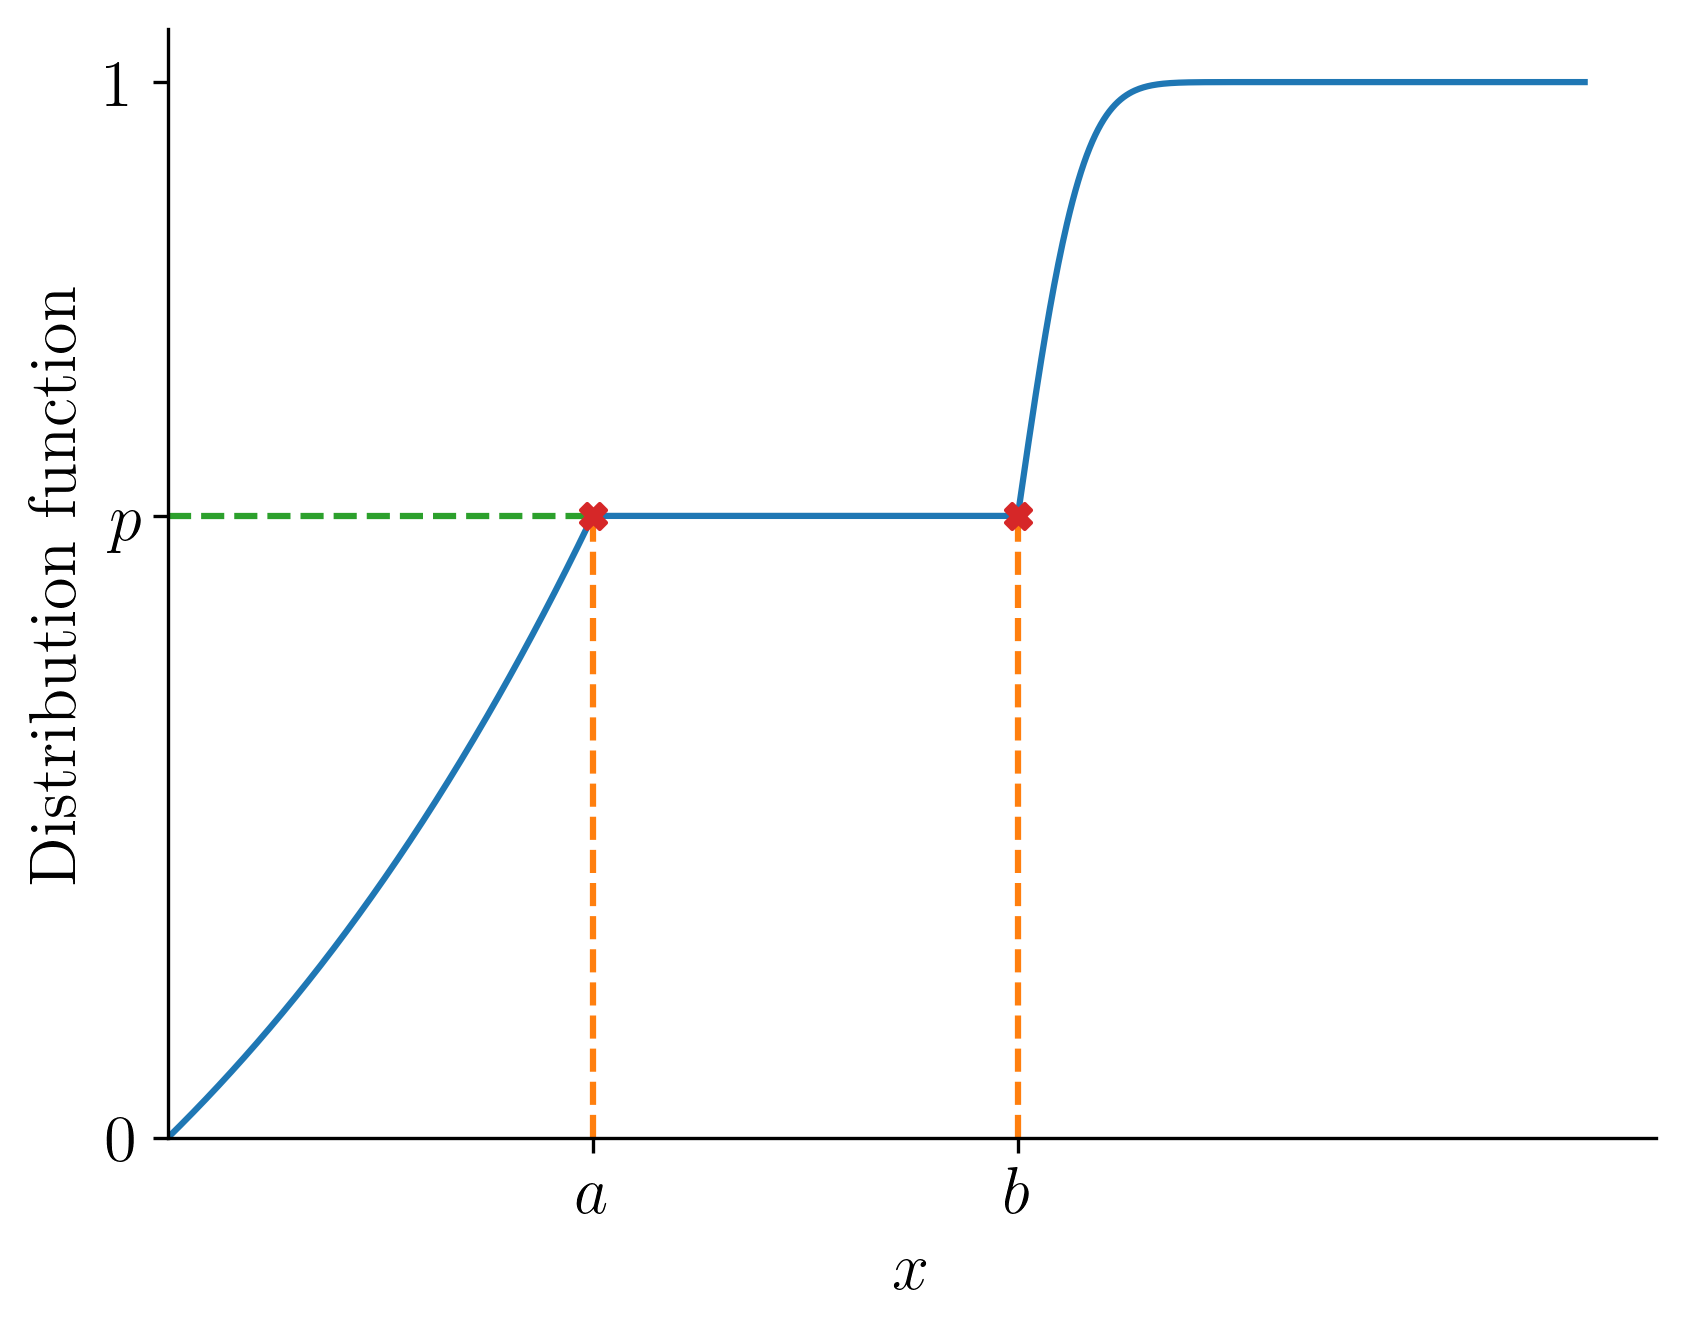
\includegraphics[width=0.5\linewidth]{./Section/Simulation/Nicht Simulierbar.png}
\caption{Verteilungsfunktion einer vermutlich schlecht simulierbaren Verteilung}
\end{figure}

Die Verteilungsfunktion ist auf $[a, b]$ nur monoton. Ist $U = p$, so ist
\begin{align*}
F^{-1}(p) &= \inf\{ x \in \mathbb{R} \mid F(x) \geq p\}\\
&= \inf\{ x \in [a, \infty)\}\\
&= a~.
\end{align*}
Die numerische Methode hingegen versucht ein $x \in \mathbb{R}$ zu finden mit $F(x) = p$ . Ist $\mathbb{E}(X) > b$, so findet die numerische Methode vermutlich zuerst den Wert $b$, womit wir dann ein falsches Ergebnis erhalten. In den allermeisten Fällen sollte dies jedoch gut gehen.
\end{Beispiel}

\newpage

Nun können wir einige Beispiele untersuchen, für die die Methode wunderbar funktioniert.

\begin{Beispiel}{(Klassische Zufallsvariablen)}
Um die Richtigkeit unserer Ergebnisse zu \glqq überprüfen\grqq{}, können wir unseren Code mit den entsprechenden Funktionen von NumPy vergleichen. Wir verwenden eine Bernoulli-Verteilung als finites, eine Poisson-Verteilung als diskretes, sowie eine Normal- und Exponentialverteilung als stetige Beispiele.\\
\begin{minipage}{0.5\linewidth}
\begin{figure}[H]
\begin{center}
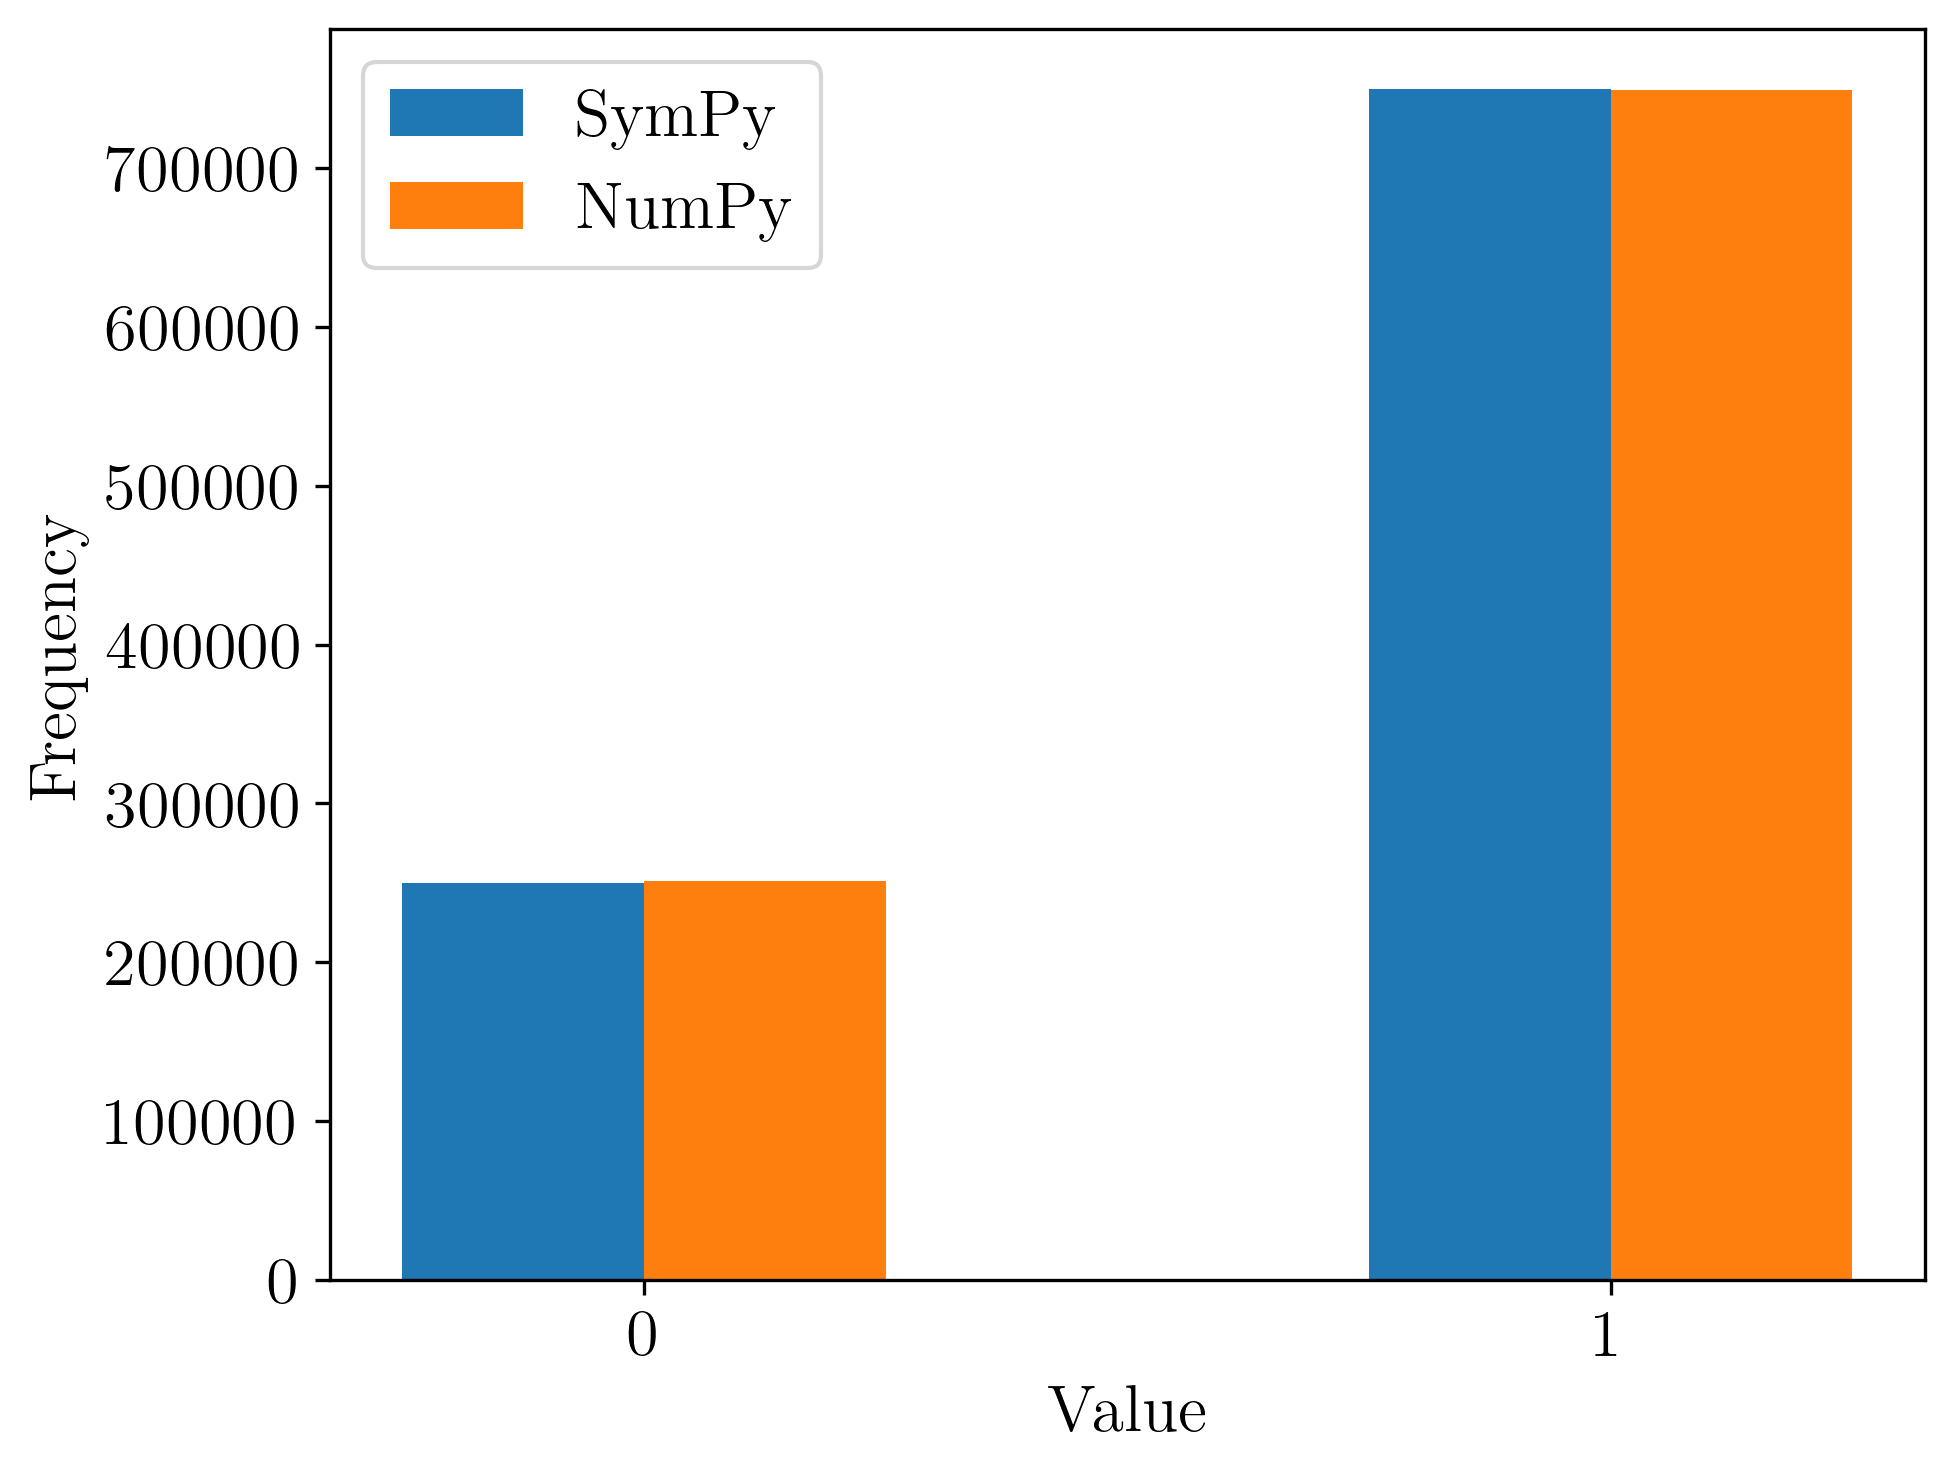
\includegraphics[width=\linewidth]{./Section/Simulation/Sim Bernoulli.png}
\caption{Simulation einer $\Ber(3/4)$-Verteilung}
\end{center}
\end{figure}
\end{minipage}
\begin{minipage}{0.5\linewidth}
\begin{figure}[H]
\begin{center}
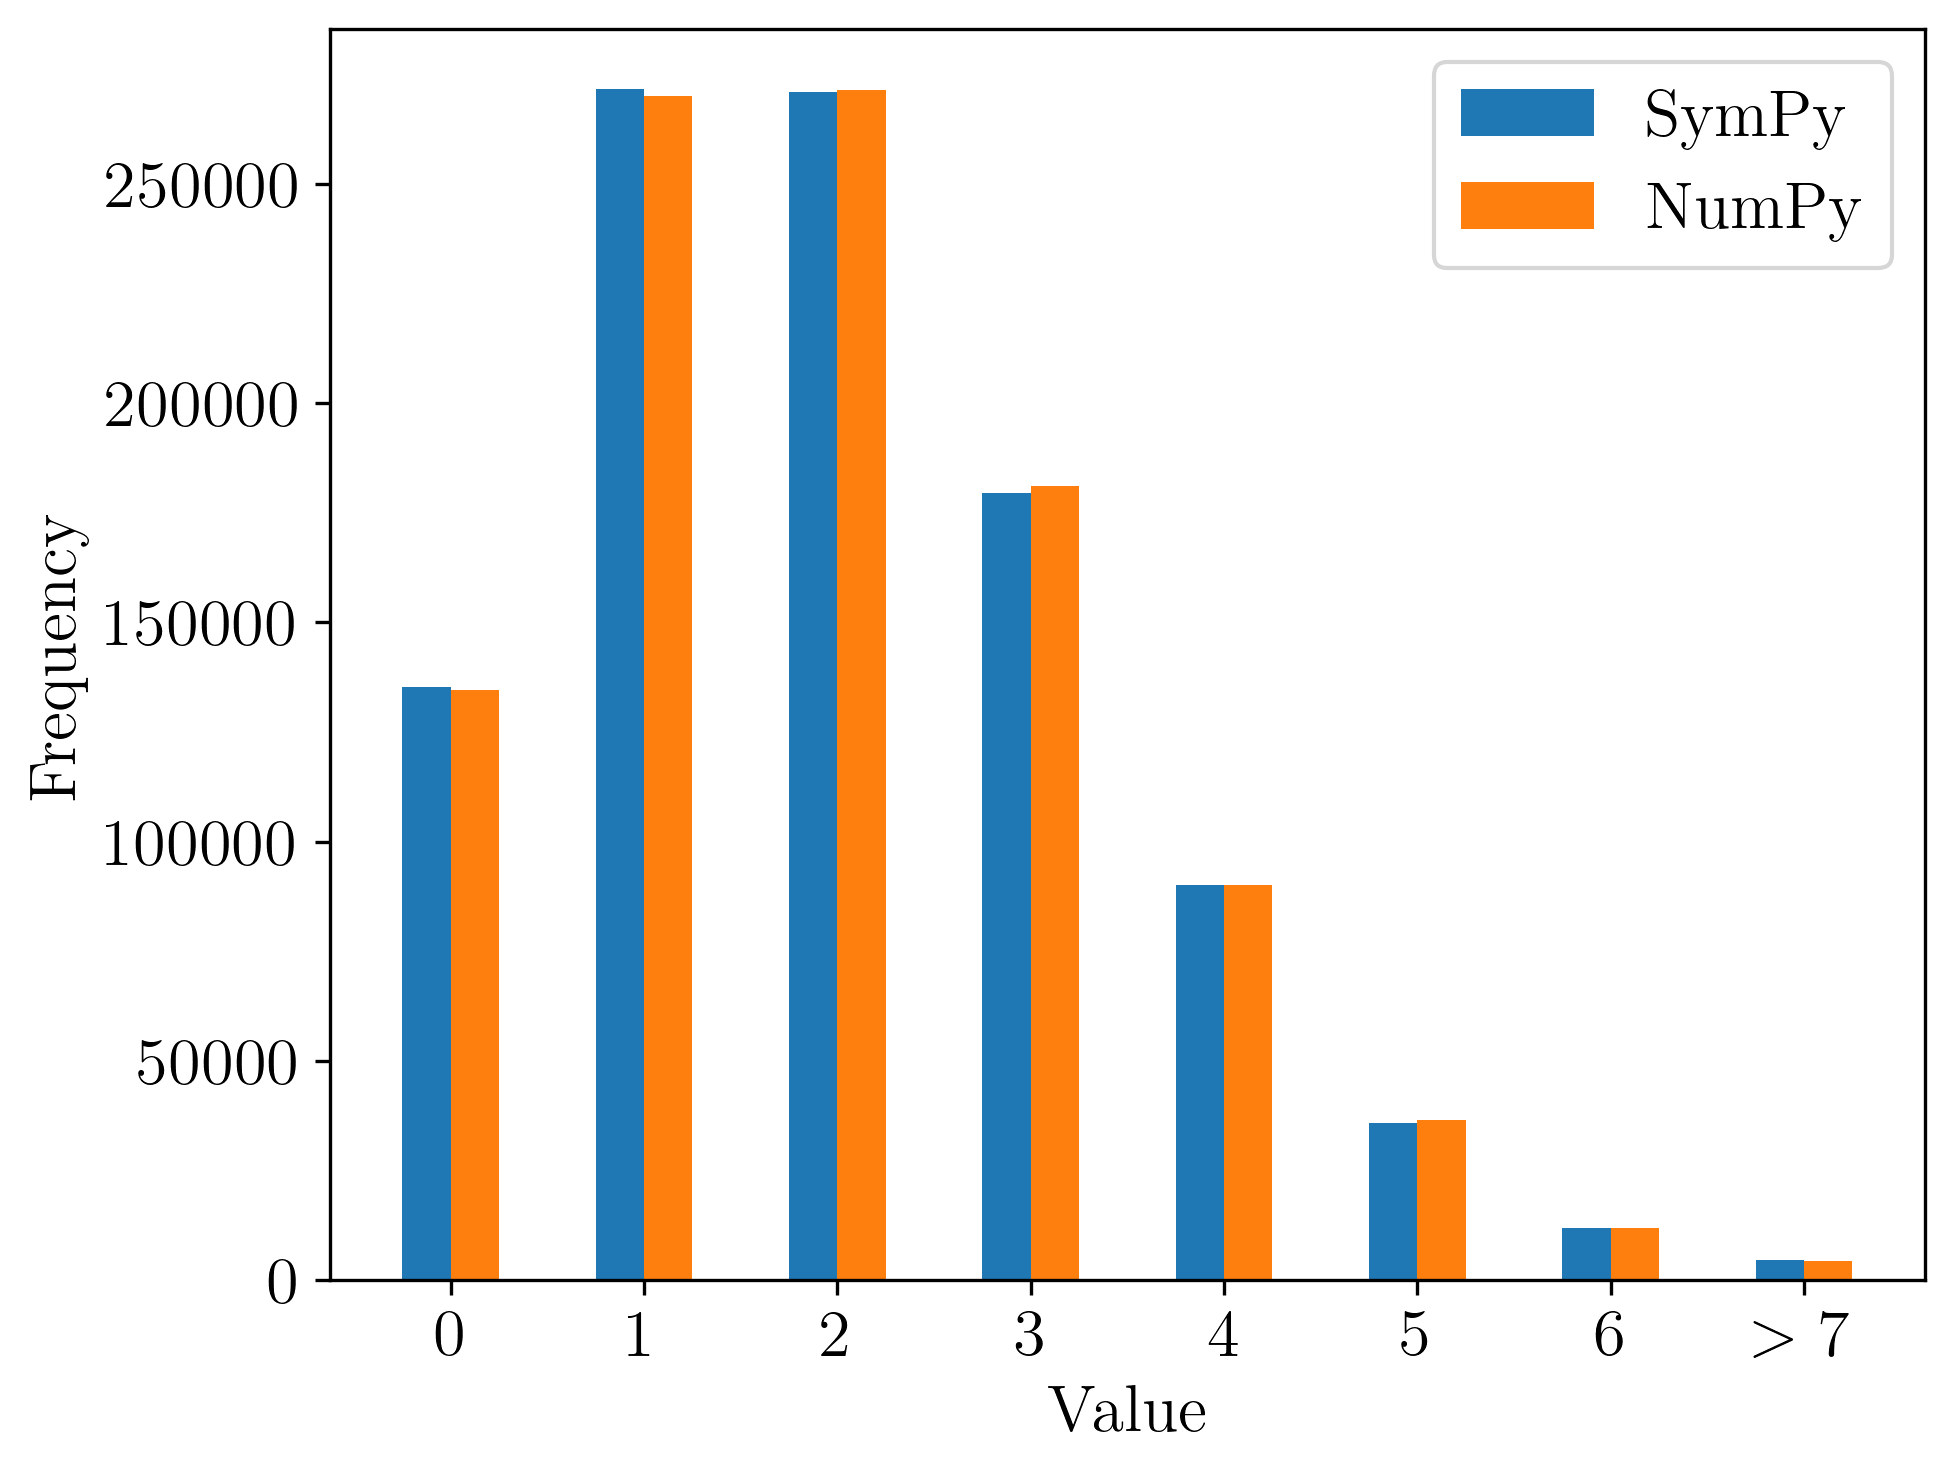
\includegraphics[width=\linewidth]{./Section/Simulation/Sim Poisson.png}
\caption{Simulation einer $\Poiss(2)$-Verteilung}
\end{center}
\end{figure}
\end{minipage}

\begin{minipage}{0.5\linewidth}
\begin{figure}[H]
\begin{center}
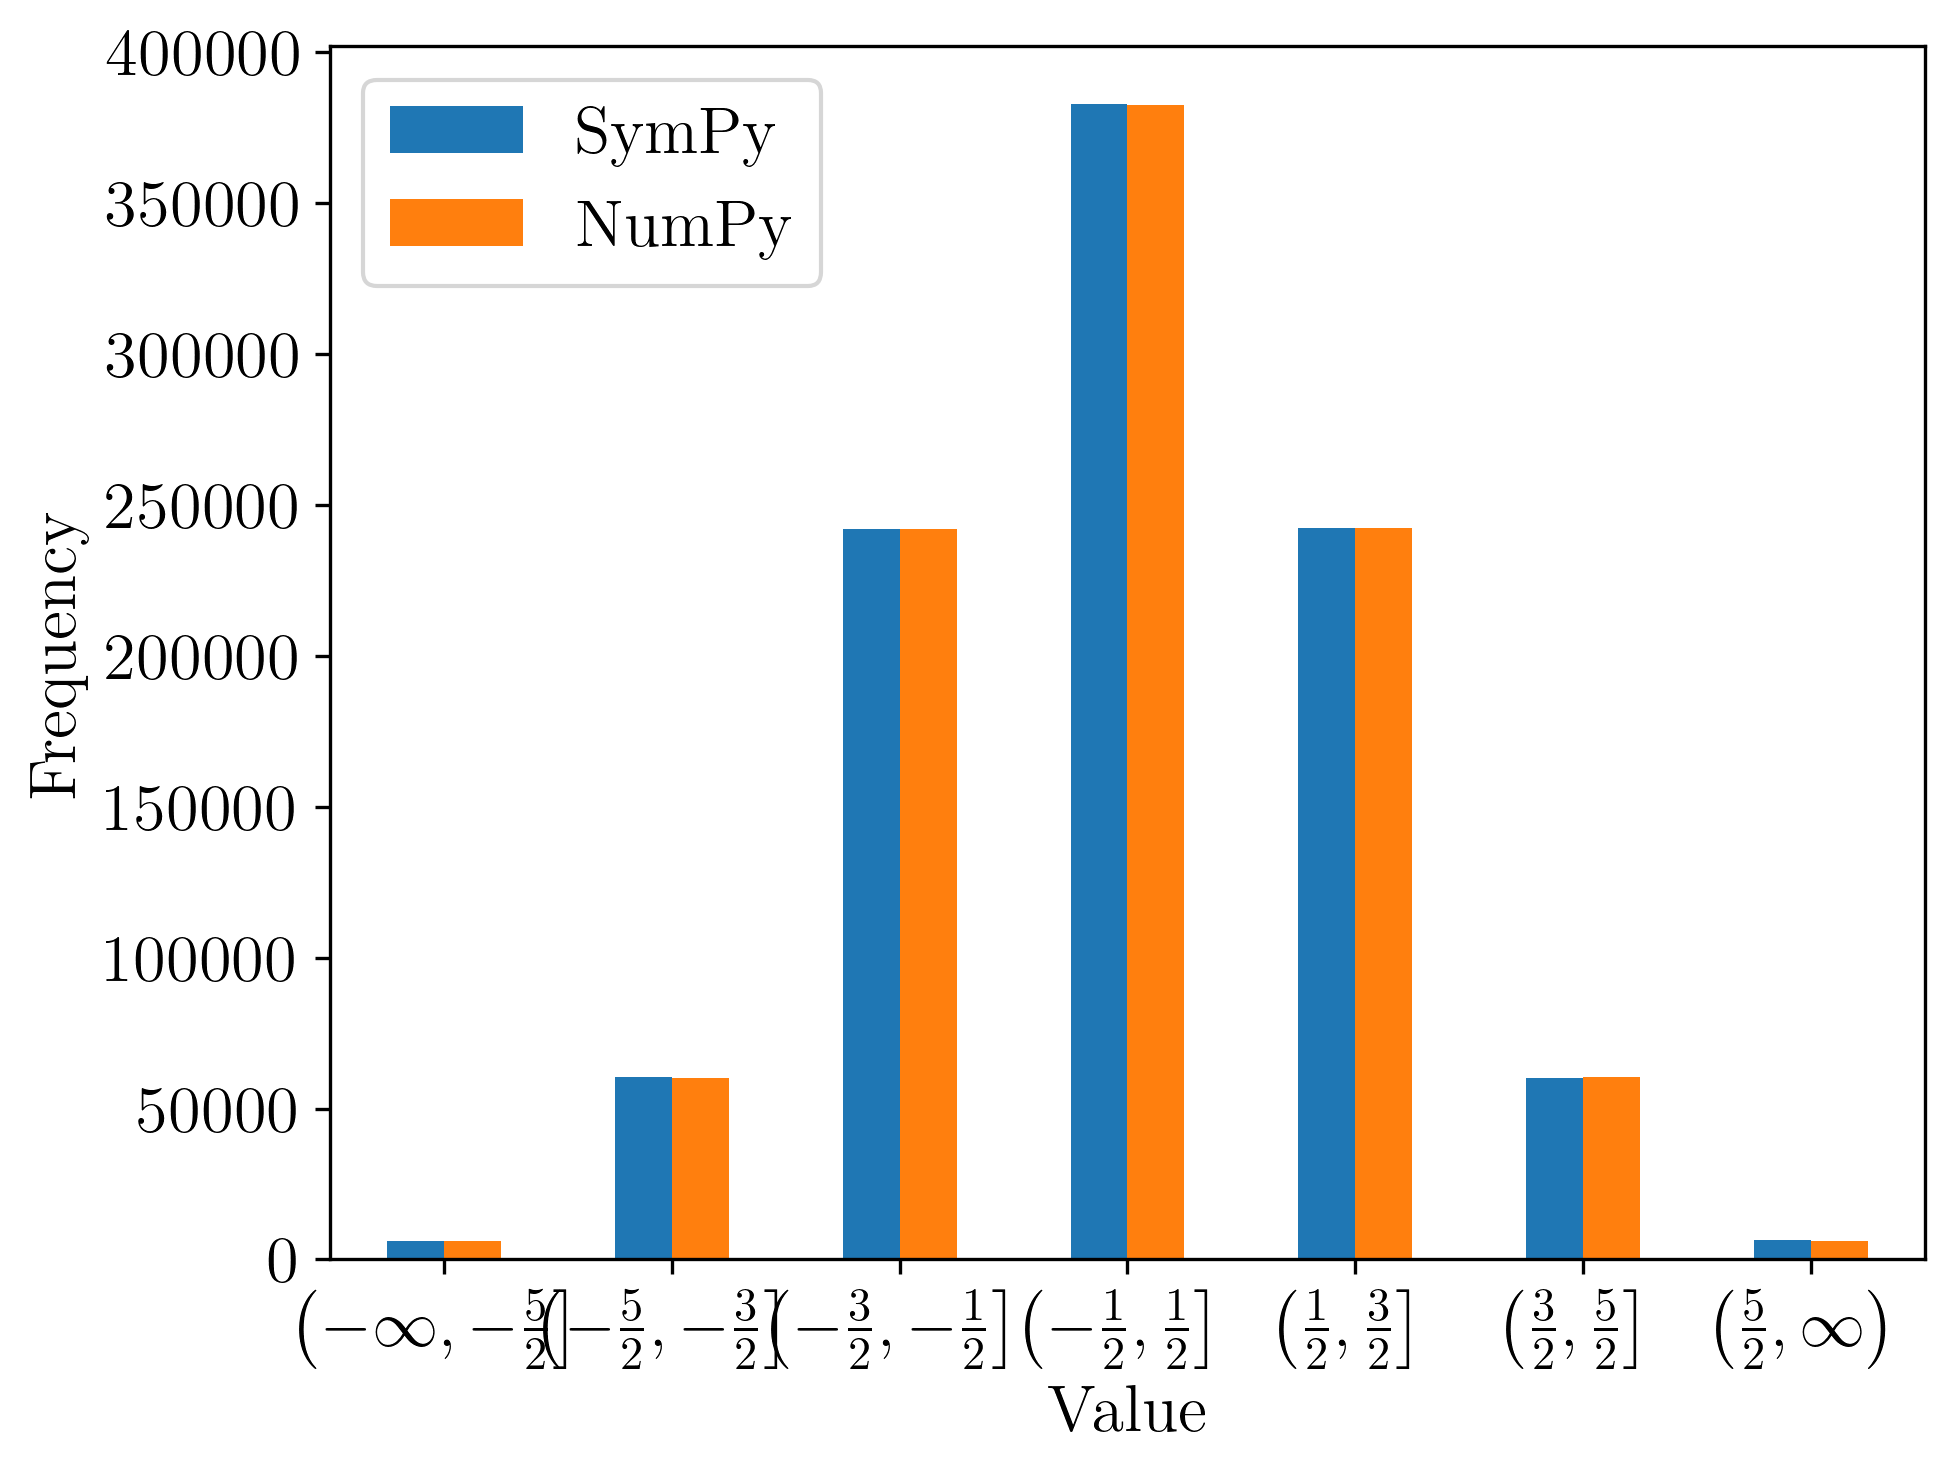
\includegraphics[width=\linewidth]{./Section/Simulation/Sim Normal.png}
\caption{Simulation einer $\Nor(0, 1)$-Verteilung}
\end{center}
\end{figure}
\end{minipage}
\begin{minipage}{0.5\linewidth}
\begin{figure}[H]
\begin{center}
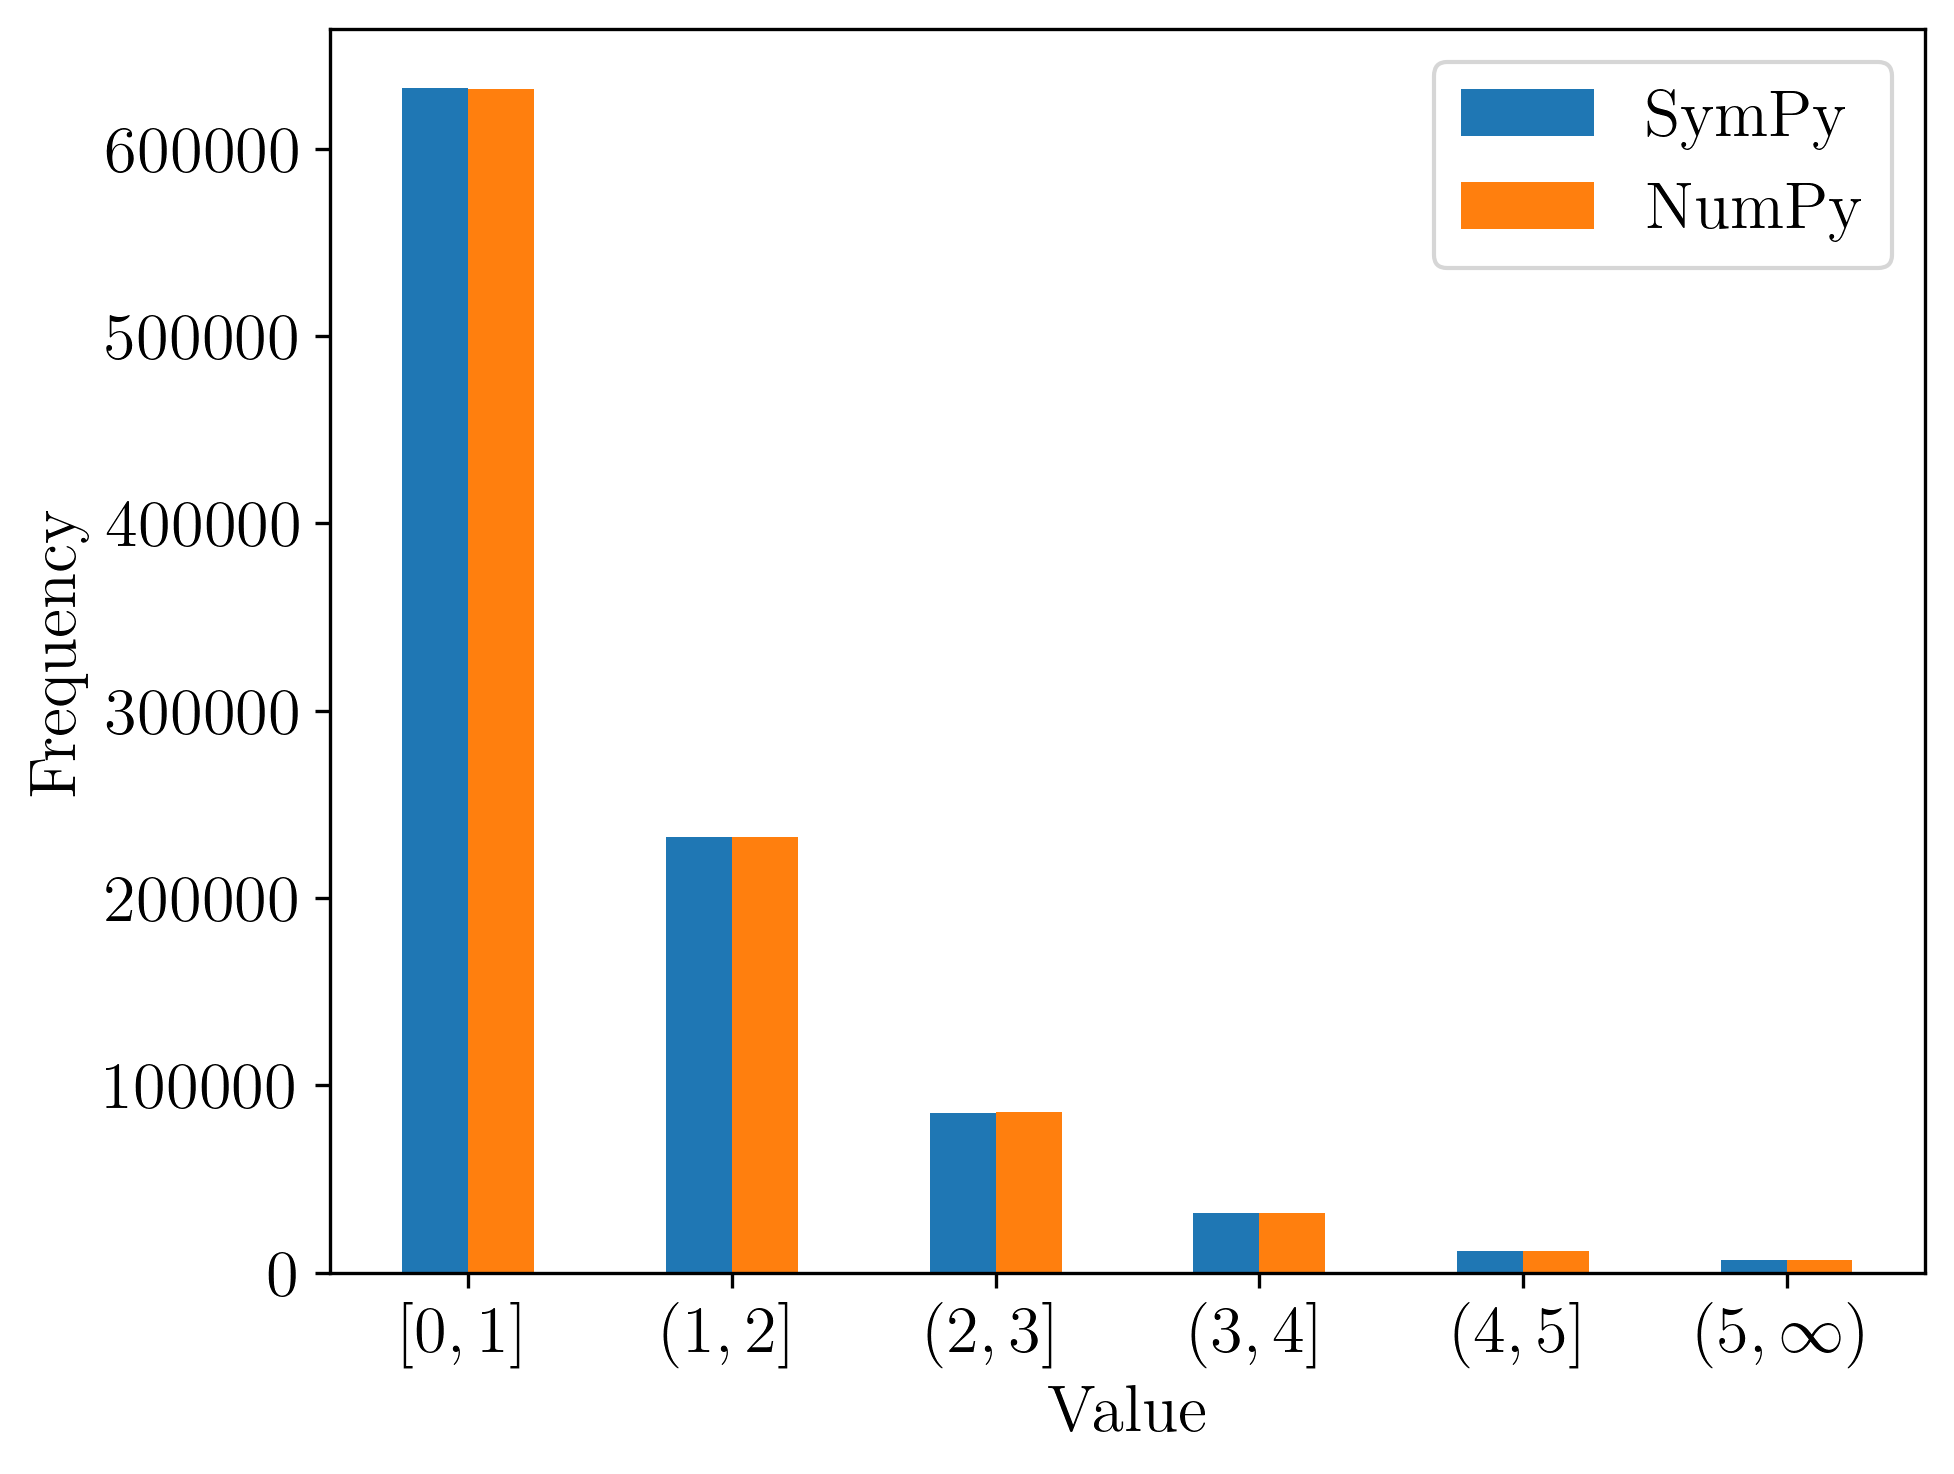
\includegraphics[width=\linewidth]{./Section/Simulation/Sim Exp.png}
\caption{Simulation einer $\Exp(3)$-Verteilung}
\end{center}
\end{figure}
\end{minipage}

Vergleicht man jeweils die Höhe benachbarter Balken miteinander, so scheint es, als würde der von uns programmierte Code genau das tun, was er soll.
\end{Beispiel}

\newpage

Als großen Vorteil gegenüber NumPy können wir die folgenden Beispiele betrachten.

\begin{Beispiel}{(Nicht-klassische Zufallsvariablen)}
Wir werden nun Zufallsvariablen simulieren, die nicht in NumPy implementiert sind und zu denen wir nur die Dichte haben.
\begin{enumerate}[label=(\roman*)]
\item Wir können an dieser Stelle das \hyperlink{Bsp:Münze}{\blue{Münzwurfbeispiel}} simulieren.
\begin{figure}[H]
\centering
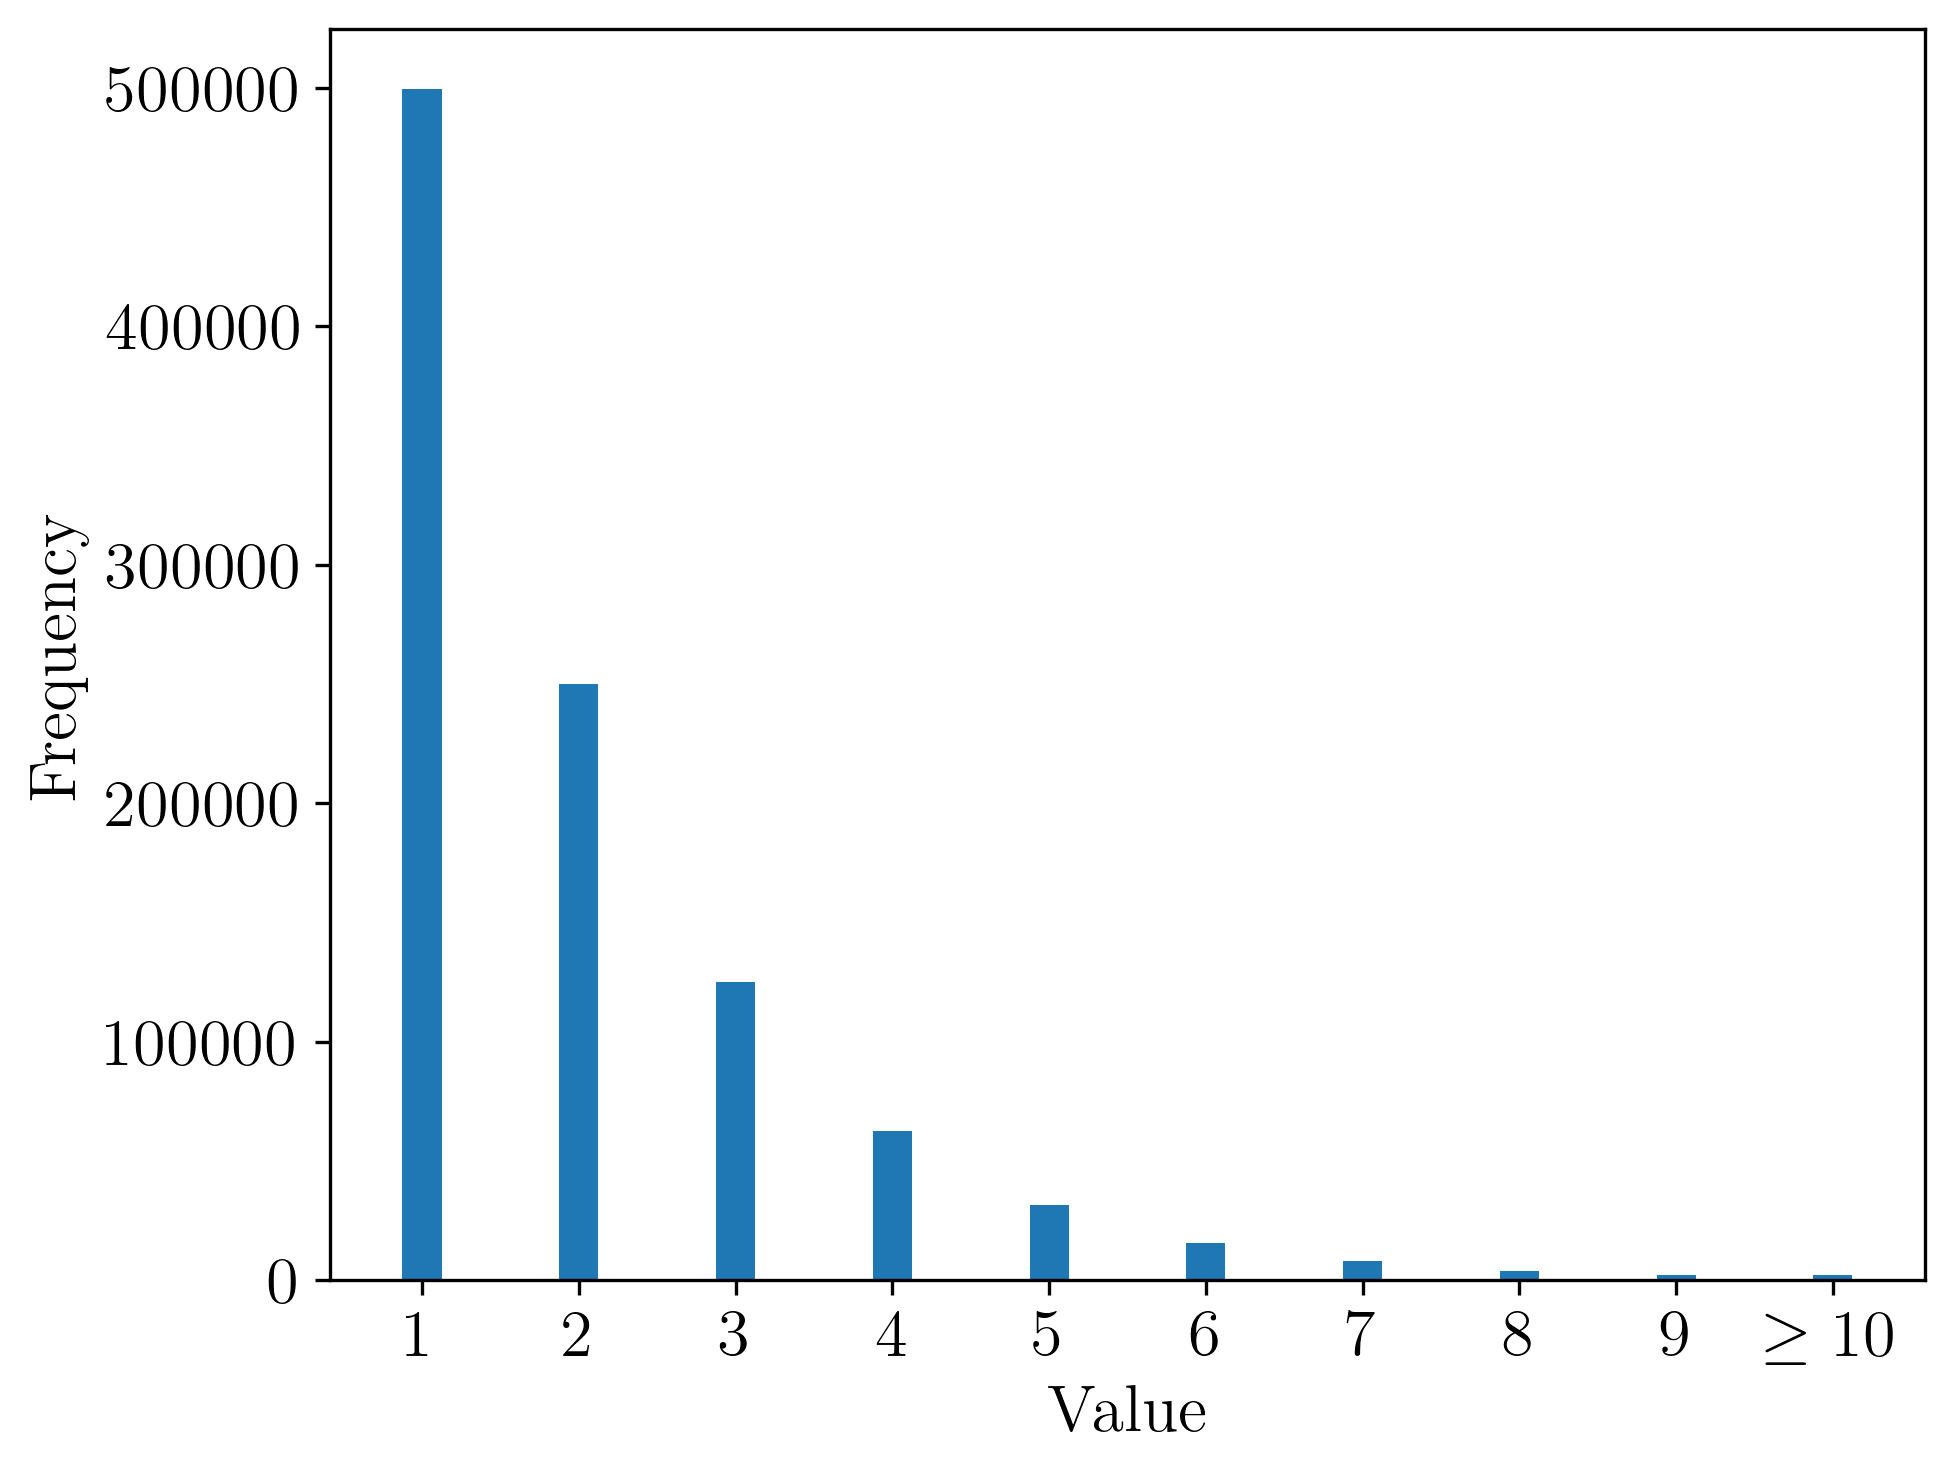
\includegraphics[width=0.5\linewidth]{./Section/Simulation/Sim Dis.png}
\caption{Simulation einer Verteilung mit Dichte $\sim 2^{- n}$}
\end{figure}
Der höchste Wert der Zufallsvariable lag bei $27$. Dieses Ereignis hat eine Wahrscheinlichkeit von
\begin{align*}
\mathbb{P}(X = 27) &= 2^{-27}\\
&= 7.4506 \cdot 10^{-9}~.
\end{align*}

\item Gegeben sei einer Verteilung mit der Dichtefunktion
\[\varphi(x) = \left(- \frac{3}{4} x^2 + \frac{3}{4}\right) \indi_{[-1, 1]}(x)~.\]
Wir können auf einfache Weise die Normiertheit nachrechnen mittels
\begin{align*}
\mathbb{P}_X(\mathbb{R}) &= \int_\mathbb{R} \left(- \frac{3}{4} x^2 + \frac{3}{4}\right) \indi_{[-1, 1]}(x) \d x\\
&= \int_{-1}^1 - \frac{3}{4} x^2 + \frac{3}{4} \d x\\
&= \left[ - \frac{1}{4} x^3 + \frac{3}{4} x \right]_{-1}^1\\
&= - \frac{1}{4} \cdot 1^3 + \frac{3}{4} \cdot 1 + \frac{1}{4} \cdot (-1)^3 - \frac{3}{4} \cdot (-1)\\
&= - \frac{1}{4} + \frac{3}{4} - \frac{1}{4} + \frac{3}{4}\\
&= 1~.
\end{align*}
Die Nullstellen von $\varphi$ sind genau an den Grenzen des Trägers, womit die Dichte überall nicht-negativ ist. Wir können nun diese Zufallsvariable simulieren und würden etwas ähnliches, wie bei der Normalverteilung erwarten, nur dass die Werte auf $[-1, 1]$ beschränkt sind.
\begin{figure}[H]
\centering
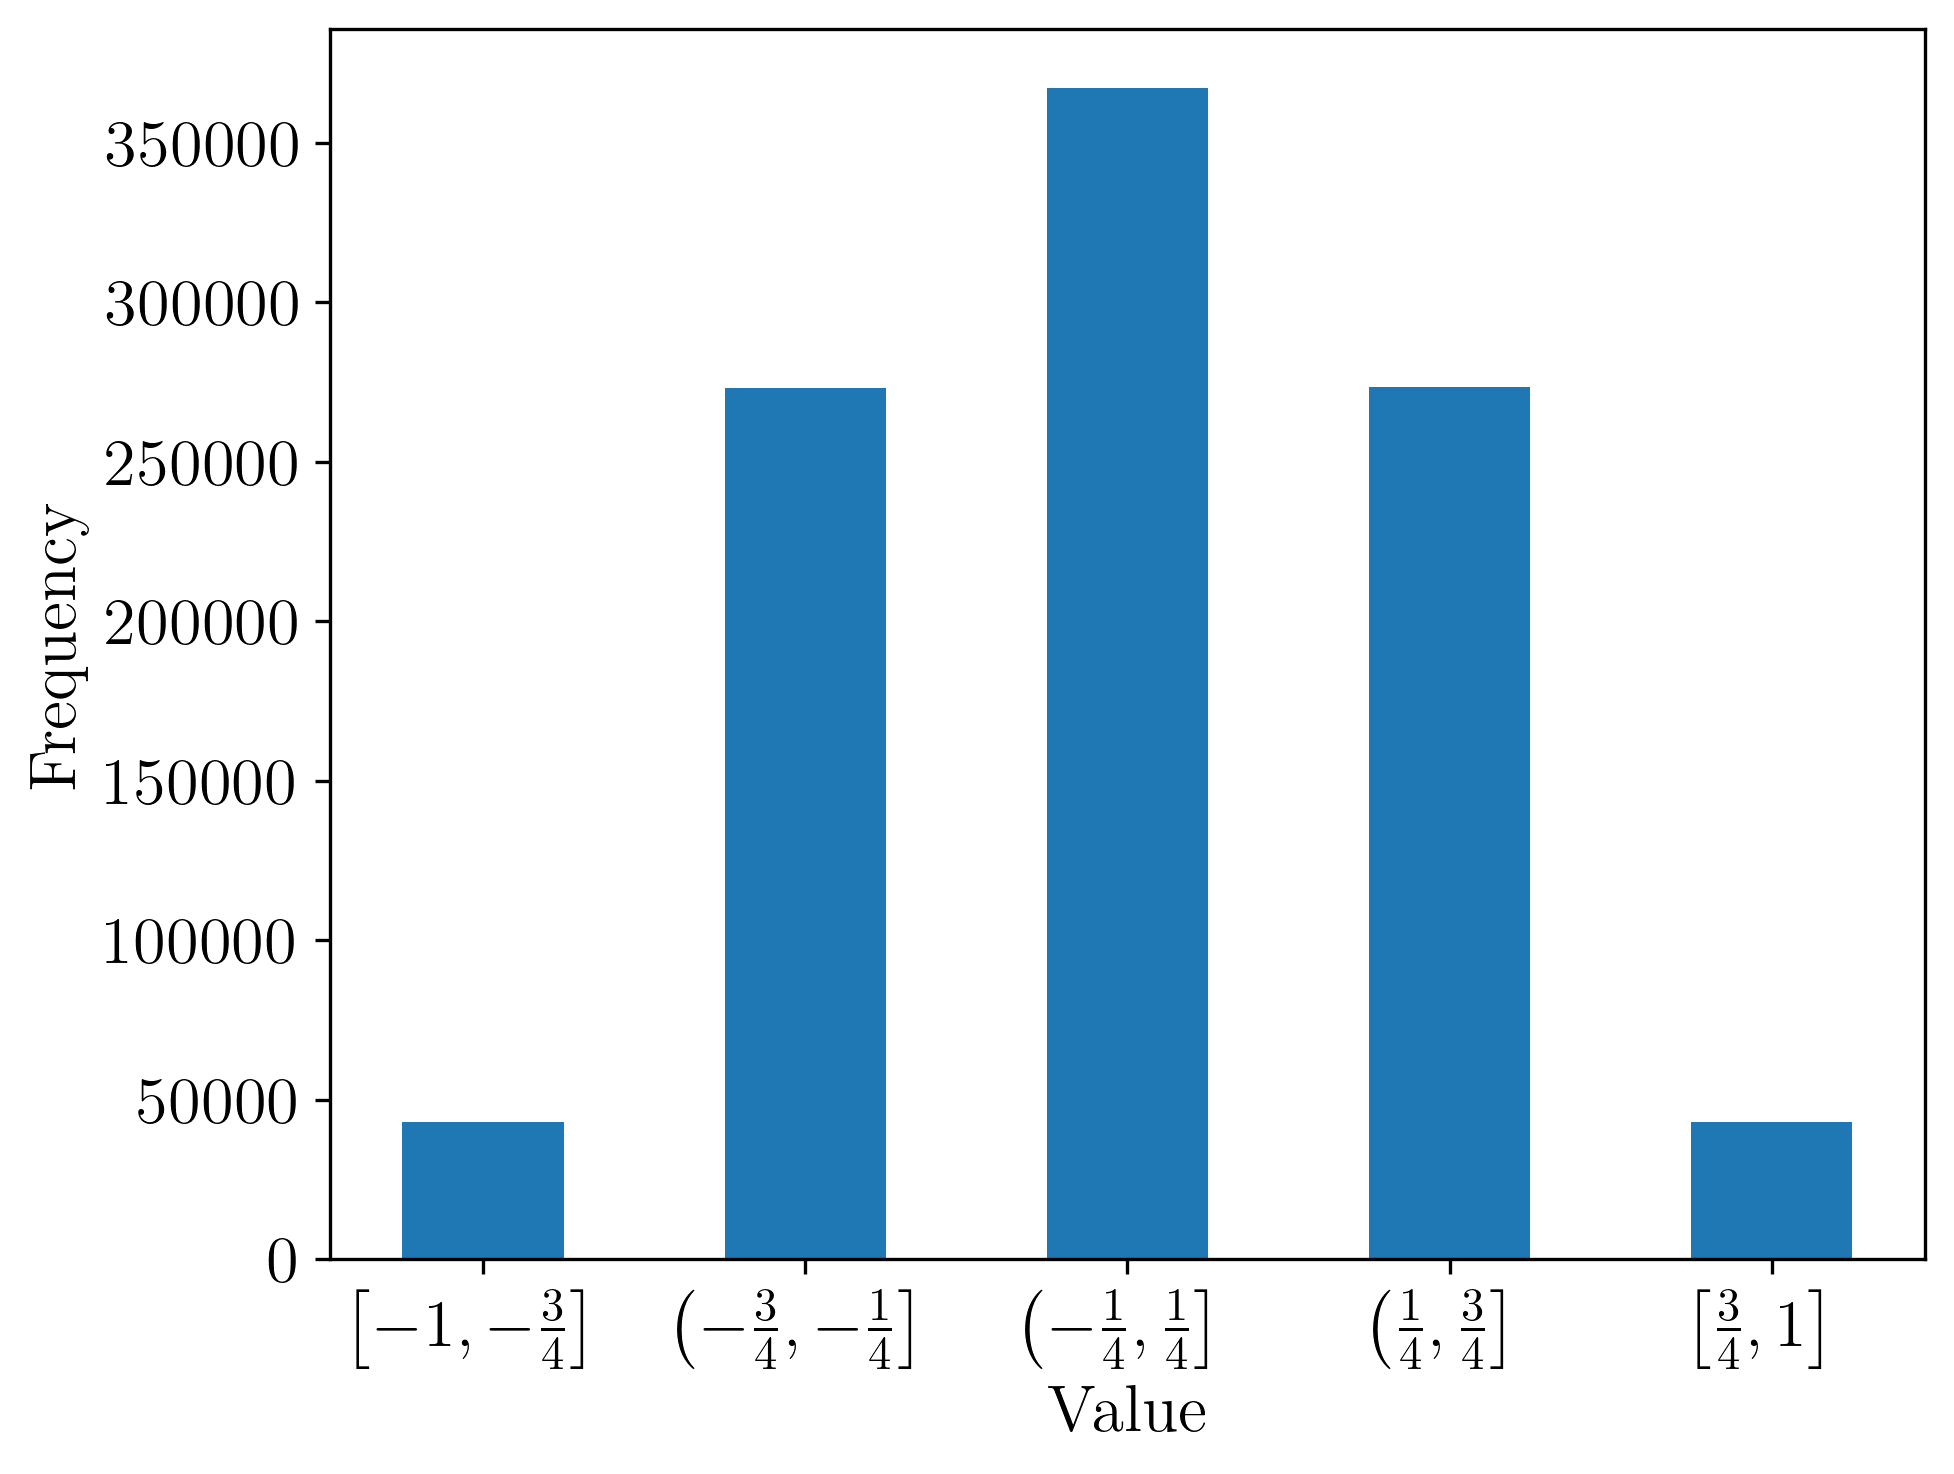
\includegraphics[width=0.5\linewidth]{./Section/Simulation/Sim Sq.png}
\caption{Simulation einer Verteilung mit Dichte $\sim - x^2$}
\end{figure}

\item Als letztes Beispiel können wir die mit der Normalverteilung verwandte, \hyperlink{Bsp:Platy}{\blue{platykurtische Verteilung}} simulieren. Wir würden wieder etwas Ähnliches zur Normalverteilung erwarten, nur dass die Enden schneller abfallen und mehr Ereignisse um die Null zentriert sind.

\begin{figure}[H]
\centering
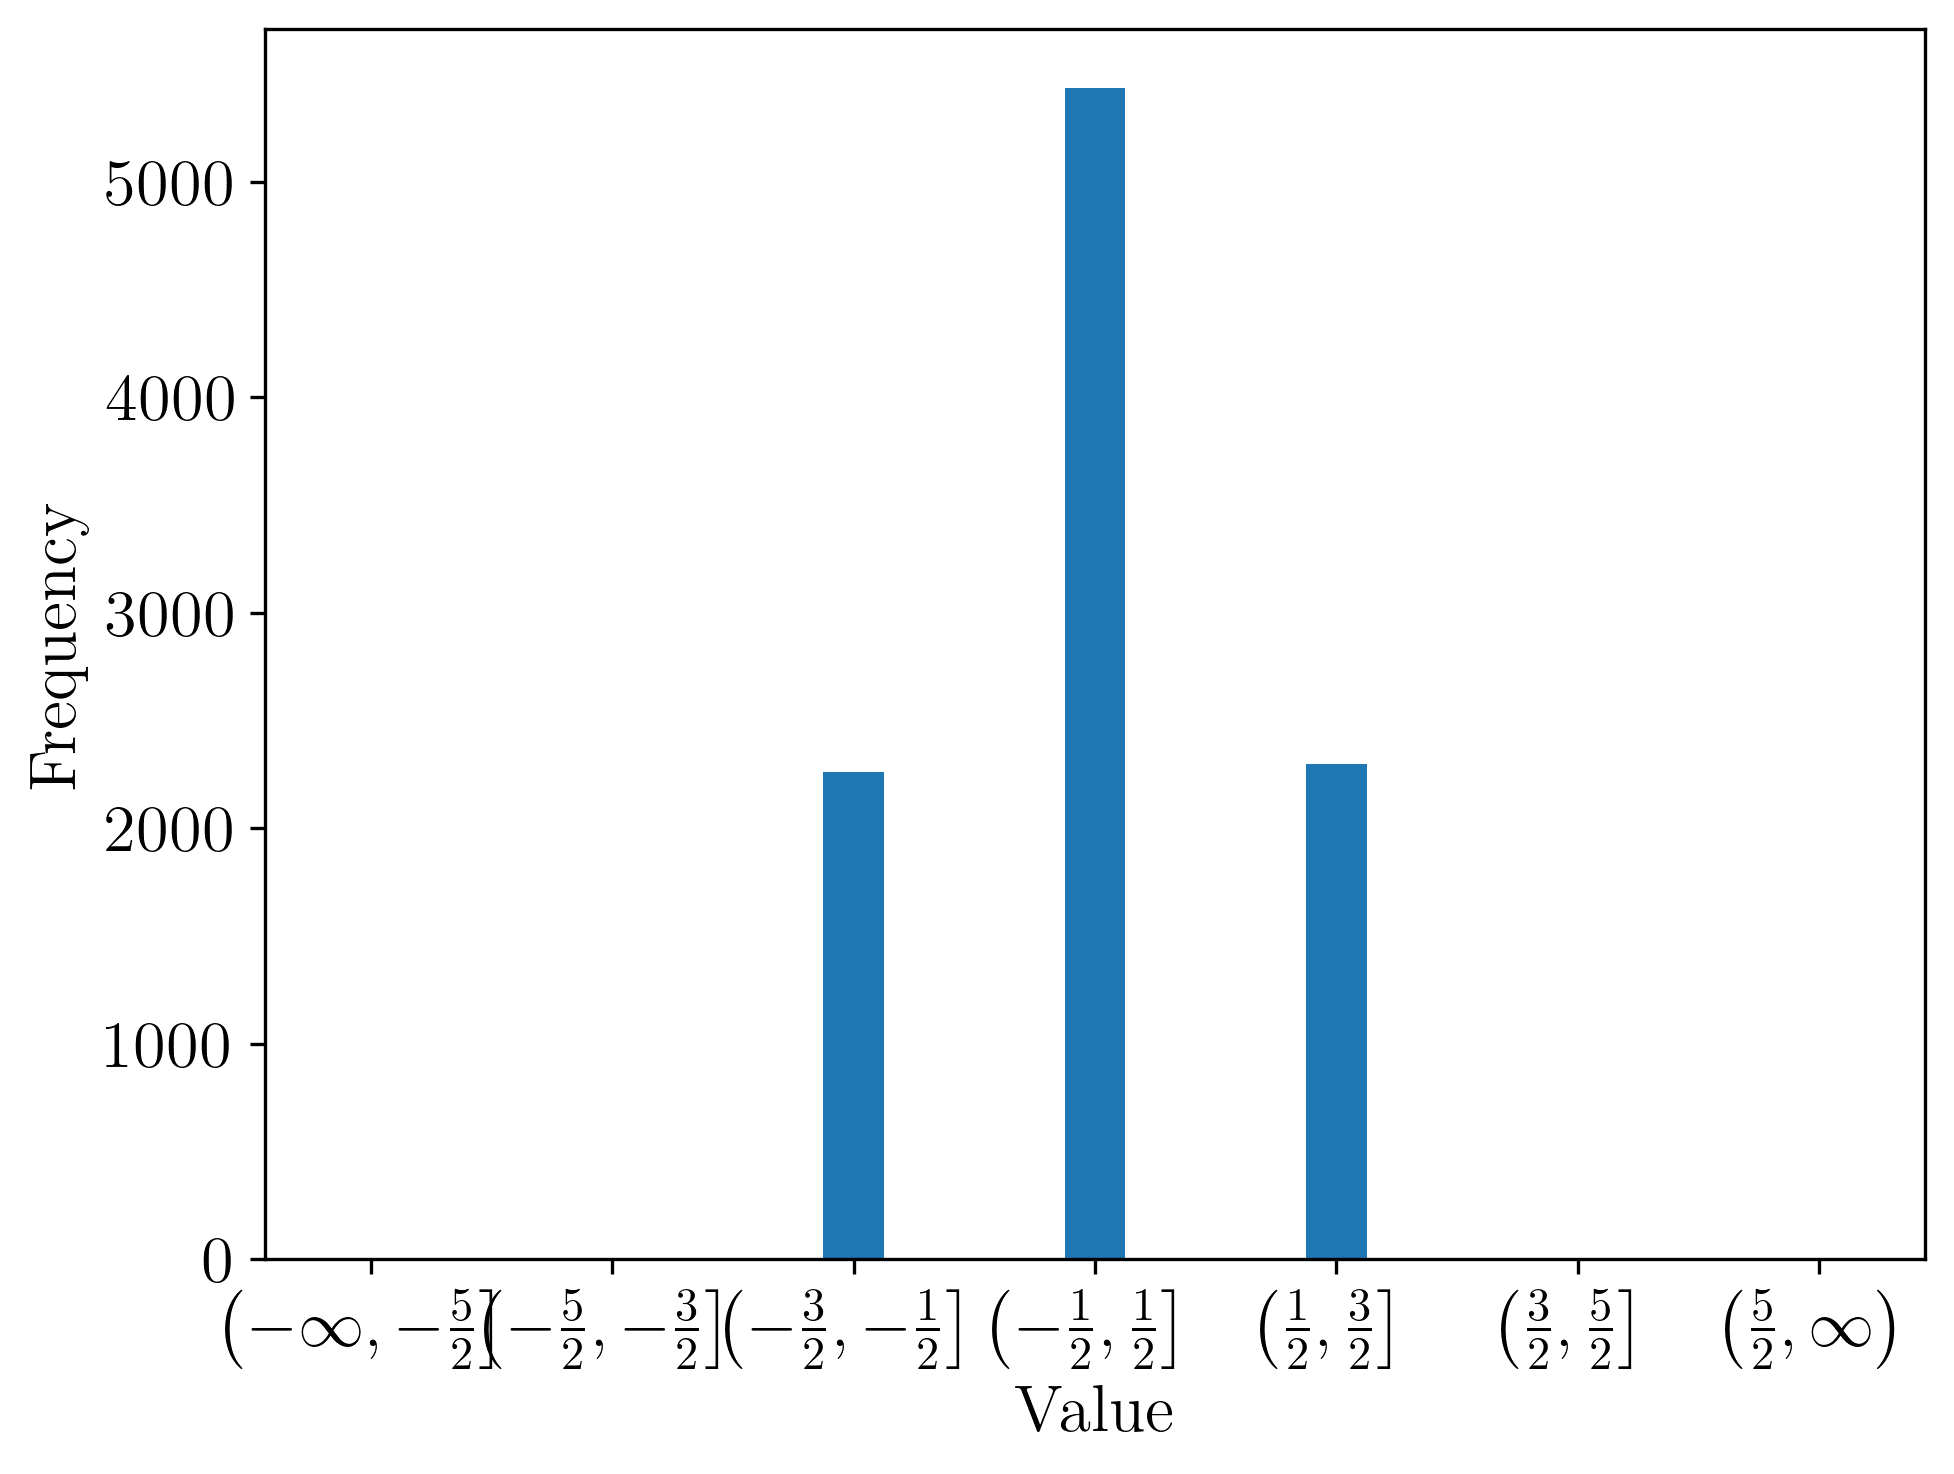
\includegraphics[width=0.5\linewidth]{./Section/Simulation/Sim Platy.png}
\caption{Simulation einer Verteilung mit Dichte $\sim \exp(- x^4)$}
\end{figure}

Da die gleiche Aufteilung auf der $x$-Achse gewählt wurde, erkennen wir genau das Vorhergesagte.
\end{enumerate}
Wir wollen es bei diesen Beispielen belassen. Insbesondere in diesem Kapitel sind der Phantasie keine Grenzen gesetzt und ich möchte Sie dazu anregen, das Programm selbst auszuprobieren.
\end{Beispiel}

\section{Mögliche Erweiterungen}

In diesem letzten Kapitel werden wir uns mit einigen möglichen Erweiterungen beschäftigen.\\

Eine wichtige Verallgemeinerung wäre es auf jeden Fall diese Bibliothek auf $d$-dimensionale Zufallsvektoren zu erweitern. Dies war anfangs auch das Ziel, doch leider stoß da SymPy auf einige Probleme. Ein großer Teil aller besprochenen Funktionen hat ohne Probleme auch für mehrdimensionale Zufallsvariablen funktioniert. Entsprechend wird beispielsweise der Erwartungswert zum Erwartungsvektor. Als großes Problem stellt sich dabei heraus, dass die Berechnung nur für Zufallsvektoren mit unabhängigen Einträgen funktionierte. Als erstes wurde eine zweidimensionale Multinormalverteilung versucht und SymPy hat ohne Ergebnis oder Fehler eine gute Stunde versucht den Erwartungswert zu berechnen. Ersetzen von $\mu_1$ und $\mu_2$ durch konkrete Zahlen erlaubte es SymPy nach langer Rechnung zumindest numerisch den Erwartungsvektor ungefähr zu berechnen. Für das nächste Beispiel wurde $X \sim \Exp(\lambda)$ und $Y \sim \Nor(\mu, \sigma)$ gewählt und der Zufallsvektor $(X, X + Y)^\top$ betrachtet. Auch hier rechnete SymPy ergebnislos für sehr lange Zeit. Da nicht einmal die Berechnung des Erwartungswertes für diese doch ziemlich einfachen Beispiele funktionierte, wurde dieser Teil nicht weiter bearbeitet.\\

Eine weitere nützliche Erweiterung wäre es zur Definition eines \lstinline|RandomVariable|-Objekts nicht mehr eine Dichte zu fordern. Man könnte also versuchen dieses Objekt mit der Verteilungs- oder charakteristischen Funktion zu definieren. Man müsste dann entsprechend die Methoden anpassen, dass diese in der Lage sind entsprechende Charakteristika auf anderen Wegen zu berechnen. Also beispielsweise
\begin{align*}
\mathbb{E}(X) &= \int_0^\infty 1 - F(x) \d x - \int_{-\infty}^0 F(x) \d x
\intertext{mit Verteilungsfunktion oder}
\mathbb{E}(X) &= \left[ \frac{\d}{\d t} \frac{C_X(t)}{i} \right]_{t = 0}
\end{align*}
mit charakteristischer Funktion. Außerdem könnte man damit eine deutlich größere Klasse an Zufallsvariablen simulieren.\\

Eine weiter schöne Erweiterung wäre es, die Python-Operatoren für Addition, Subtraktion, Multiplikation und Division zu implementieren. Damit könnte man dann zwei \lstinline|RandomVariable|-Objekte addieren, um daraus ein Neues zu erhalten. Da die Dichte der Summe von Zufallsvariablen deren Faltung ist, müsste man eine entsprechende Faltungsmethode definieren. Damit könnte man dann vielleicht entsprechende Sätze über die Summe von unabhängigen (identisch verteilten) Zufallsvariablen \glqq zeigen\grqq{} oder eine Brücke zu stochastischen Prozessen schlagen.\\

Umgekehrt gäbe es die Möglichkeit einer Spezialisierung. Man könnte für häufig vorkommende Verteilungen, wie zum Beispiel der Normalverteilung eine Unterklasse erstellen, die dann manche Berechnungen nicht mehr durchführen muss, um Rechenaufwand zu sparen. Beispielsweise verschwinden die ungeraden Momente einer Standardnormalverteilung aus Symmetriegründen. SymPy sieht dies leider nicht immer und berechnet deshalb das entsprechende Integral ohne abzukürzen. Durch die Unterklasse könnte man sich diese Berechnung ersparen. Die Implementierung von diesen Unterklassen hätte dann auch den Vorteil, dass Eingaben einfacher werden würden. Momentan muss man die ganzen Dichten und Symbole mit SymPy manuell definieren. Für diese Unterklassen wäre das dann alles schon programmiert und für ein Normalverteilungsobjekt müsste man nur ein $\mu$ und ein $\sigma$ angeben.\\

Sehr interessant wäre es zudem einen vierten Typen der Zufallsvariablen zu implementieren, der deutlich abstrakter ist. Man müsste zuerst eine Klasse auf die \lstinline|sym.Function|-Klasse aufbauen, die Dichtefunktionen beschreibt. Für diese Dichtefunktionen sollte man einen allgemeinen Integralbegriff implementieren, der Eigenschaften wie Linearität besitzt und für den man
\[\int \varphi \d \mathbb{P} = 1\]
definiert. Mit Dichtefunktions-Klasse könnte man dann eine \lstinline|RandomVariableAbstract|-Klasse definieren, mit der man vielleicht mehr Sätze, wie in der Bachelorarbeit angedeutet, mit SymPy \glqq beweisen\grqq{} kann.\\

Ein wichtiger Teil, der in meinem Programm recht wenig Beachtung gefunden hat, ist das Exception Handling. Damit der Code nicht allzu umfangreich wird und da dieses Programm eher als proof-of-concept gedacht ist, wurde auf derartige Überprüfungen verzichtet. Man kann beispielsweise in die \lstinline|moment|-Methode ohne Probleme eine negative Zahl oder Brüche reinstecken und wird dann vermutlich einen schwierig interpretierbaren Fehler von SymPy erhalten. Um dies zu verbessern, müssten also in jede Methode entsprechende \lstinline|try|- und \lstinline|except|-Blöcke eingebaut werden, die diese Fehler herausfiltern.\\

Abschließend denke ich, dass mit dieser Arbeit ein gut funktionierender Grundstein für vielfältige Erweiterungen gelegt wurde.

\section{Anhang}
\hypertarget{Sec:Anhang}{}

Hier der Code von \lstinline|RandomVariableFinite.py|
\begin{small}
\begin{lstlisting}
import sympy as sym
import numpy as np
import matplotlib.pyplot as plt

from .RandomVariable import RandomVariable


class RandomVariableFinite(RandomVariable):
    def __init__(self, density, variables, force_density=False):
        """
        A subclass of RandomVariable for finite random variables.

        Parameters:
            density (dict): The density function of the random variable as a dictionary mapping values to probabilities.
            variables (sympy.Symbol): The symbol used in the density function as a sympy object.
            force_density (bool): An Argument for skipping the check if the density function is normalized. Default is False.
        """
        self.type = 'f'
        density = RandomVariableFinite._make_density(density)
        # Initiates Random Variable
        super(RandomVariableFinite, self).__init__(density, variables, force_density=force_density)

    @staticmethod
    def _make_density(old_density):
        """
        Converts the density function of the random variable to a sympy expression if necessary.

        Parameters:
            old_density (dict): The density function of the random variable as a dictionary mapping values to probabilities.

        Returns:
            dict: The density function of the random variable as a dictionary mapping sympy expressions to sympy expressions.
        """
        density = {}
        for key in old_density.keys():
            density.update({sym.sympify(key): sym.sympify(old_density[key])})
        return density

    def integrate_random_variable(self, expr, lower=-sym.oo, upper=sym.oo):
        """
        Returns the sum of an expression involving the random variable.

        Parameters:
            expr (sympy.Expr): The expression to be summed as a symbolic expression.
            lower (sympy.Expr): The lower bound of the summation. Default is -sym.oo.
            upper (sympy.Expr): The upper bound of the summation. Default is sym.oo.

        Returns:
            sympy.Expr: The sum as a symbolic expression.
        """
        integral = sym.Integer(0)
        for key in self.density.keys():
            # Only values inside intervall
            if key >= lower and key <= upper:
                integral += expr.subs(self.variable, key) * self.density[key]
        integral = sym.simplify(integral)
        return integral

    def distribution_function(self):
        """
        Returns the distribution function of the random variable.

        Returns:
            dict: The distribution function of the random variable as a dictionary mapping values to cumulative probabilities.
        """
        sortable = True
        keys = list(self.density.keys())
        for key in keys:
            if isinstance(key, sym.Symbol):
                print('WARNING: Can\'t sort values.')
                sortable = False
                break
        if sortable:
            keys = sorted(keys)
        cumulative_probability = self.density[keys[0]]
        distribution_function = {keys[0]: cumulative_probability}
        keys.pop(0)
        for key in keys:
            cumulative_probability += self.density[key]
            distribution_function.update({key: cumulative_probability})
        return distribution_function

    def entropy(self):
        """
        Returns the entropy of the random variable.

        Returns:
            sympy.Expr: The entropy as a symbolic expression.
        """
        entropy = sym.Integer(0)
        for probability in self.density.values():
            entropy += probability * sym.log(probability)
        entropy = - entropy
        entropy = sym.simplify(entropy)
        return entropy

    def plot_density(self, show=True, use_latex=True):
        """
        Plots the density function of the random variable.

        Parameters:
            show (bool): A flag to indicate whether to show the plot or return the figure and axis objects. Default is True.
            use_latex (bool): A flag to indicate whether to use LaTeX for rendering the plot labels. Default is True.

        Returns:
            matplotlib.figure.Figure, matplotlib.axes.Axes: The figure and axis objects of the plot, if show is False.
        """
        if self._test_for_symbols():
            return
        x_values = list(self.density.keys())
        y_values = list(self.density.values())
        if use_latex:
            plt.rc('text', usetex=True)
        fig, ax = plt.subplots()
        ax.set_xlabel(f'${sym.latex(self.variable)}$')
        ax.set_ylabel('Density function')
        ax.scatter(x_values, y_values, marker='.')
        if show:
            plt.show()
        else:
            return fig, ax

    def plot_distribution_function(self, show=True, use_latex=True):
        """
        Plots the distribution function of the random variable.

        Parameters:
            lower (float or None): The lower bound of the plot domain. Default is None.
            upper (float or None): The upper bound of the plot domain. Default is None.
            show (bool): A flag to indicate whether to show the plot or return the figure and axis objects. Default is True.
            use_latex (bool): A flag to indicate whether to use LaTeX for rendering the plot labels. Default is False.

        Returns:
            matplotlib.figure.Figure, matplotlib.axes.Axes: The figure and axis objects of the plot, if show is False.
        """
        if self._test_for_symbols():
            return
        distribution_function = self.distribution_function()
        keys = list(distribution_function.keys())
        min_value = min(keys)
        max_value = max(keys)
        distance = max_value - min_value
        # Broader Plot
        lower = min_value - 0.1 * distance
        upper = max_value + 0.1 * distance
        if use_latex:
            plt.rc('text', usetex=True)
        fig, ax = plt.subplots()
        ax.set_xlabel(f'${sym.latex(self.variable)}$')
        ax.set_ylabel('Distribution function')
        # 0 from - infinity to first value
        ax.hlines(y=0, xmin=lower, xmax=min_value, color='tab:blue', linewidth=2)
        # 1 from last value to infinity
        ax.hlines(y=1, xmin=max_value, xmax=upper, color='tab:blue', linewidth=2)
        for num, key in enumerate(keys):
            # Skips last line
            if num < len(keys) - 1:
                ax.hlines(y=distribution_function[key], xmin=keys[num], xmax=keys[num+1], color='tab:blue', linewidth=2)
        if show:
            plt.show()
        else:
            return fig, ax

    def simulate(self, number):
        """
        Simulates the random variable using inverse transform sampling.

        Parameters:
            number (int): The number of samples to generate.

        Returns:
            list: A list of simulated values of the random variable.
        """
        simulate = []
        uni = np.random.uniform(0, 1, number)
        distribution_function = self.distribution_function()
        for num in uni:
            for key in distribution_function.keys():
                if num <= float(distribution_function[key]):
                    simulate.append(float(key))
                    break
        return simulate
\end{lstlisting}
\end{small}

Hier der Code von \lstinline|RandomVariableDiscrete.py|
\begin{small}
\begin{lstlisting}
import sympy as sym
import numpy as np
import matplotlib.pyplot as plt

from .RandomVariable import RandomVariable


class RandomVariableDiscrete(RandomVariable):
    def __init__(self, density, variables, supp=[], force_density=False):
        """
        A subclass of RandomVariable for discrete random variables.

        Parameters:
            density (sympy.Expr): The density function of the random variable as a symbolic expression.
            variables (sympy.Symbol): The symbol used in the density function as a sympy object.
            supp (list): The support of the density function as a list of two elements. Default is [sym.Integer(0), sym.oo].
            force_density (bool): An Argument for skipping the check if the density function is normalized. Default is False.
        """
        self.type = 'd'
        if supp == []:
            self.supp = [sym.Integer(0), sym.oo]
        else:
            self.supp = supp
        # Initiates Random Variable
        super(RandomVariableDiscrete, self).__init__(density, variables, force_density=force_density)

    def integrate_random_variable(self, expr, lower=sym.Integer(0), upper=sym.oo):
        """
        Returns the sum of an expression involving the random variable.

        Parameters:
            expr (sympy.Expr): The expression to be summed as a symbolic expression.
            lower (sympy.Expr): The lower bound of the summation. Default is sym.Integer(0).
            upper (sympy.Expr): The upper bound of the summation. Default is sym.oo.

        Returns:
            sympy.Expr: The sum as a symbolic expression.
        """
        lower = sym.Max(lower, self.supp[0])
        upper = sym.Min(upper, self.supp[1])
        integral = sym.summation(expr * self.density, (self.variable, lower, upper)).doit()
        integral = RandomVariable.clean_piecewise(integral)
        integral = sym.simplify(integral)
        return integral

    def distribution_function(self, value=None):
        """
        Returns the distribution function of the random variable.

        Parameters:
            value (float or None): The value at which to evaluate the distribution function. Default is None.

        Returns:
            sympy.Expr or float: The distribution function as a symbolic expression if value is None, or as a numerical value if value is given.
        """
        # Purely symbolic calculation
        if value == None:
            t = sym.Symbol('t', real=True)
            upper = sym.Min(self.supp[1], sym.floor(t))
            distribution_function = self.integrate_random_variable(sym.Integer(1), upper=upper)
            return distribution_function
        # Numeric calculation
        else:
            value = sym.sympify(value)
            upper = sym.Min(self.supp[1], sym.floor(value))
            distribution_function = self.integrate_random_variable(sym.Integer(1), upper=upper)
            distribution_function = float(distribution_function.evalf())
            return distribution_function

    def plot_density(self, lower=0, upper=10, show=True, use_latex=True):
        """
        Plots the density function of the random variable.

        Parameters:
            lower (int): The lower bound of the plot domain. Default is 0.
            upper (int): The upper bound of the plot domain. Default is 10.
            show (bool): A flag to indicate whether to show the plot or return the figure and axis objects. Default is True.
            use_latex (bool): A flag to indicate whether to use LaTeX for rendering the plot labels. Default is True.

        Returns:
            matplotlib.figure.Figure, matplotlib.axes.Axes: The figure and axis objects of the plot, if show is False.
        """
        if self._test_for_symbols():
            return
        x_values = np.arange(lower, upper + 1, step=1, dtype=int)
        y_values = []
        for x_value in x_values:
            # Value inside support
            if x_value >= self.supp[0] and x_value <= self.supp[1]:
                y_value = float(self.density.subs(self.variable, x_value).evalf())
            # Value inside support
            else:
                y_value = 0
            y_values.append(y_value)
        if use_latex:
            plt.rc('text', usetex=True)
        fig, ax = plt.subplots()
        ax.set_xlabel(f'${sym.latex(self.variable)}$')
        ax.set_ylabel('Density function')
        ax.scatter(x_values, y_values, marker='.')
        if show:
            plt.show()
        else:
            return fig, ax

    def plot_distribution_function(self, lower=0, upper=10, show=True, use_latex=True):
        """
        Plots the distribution function of the random variable.

        Parameters:
            lower (int): The lower bound of the plot domain. Default is 0.
            upper (int): The upper bound of the plot domain. Default is 10.
            show (bool): A flag to indicate whether to show the plot or return the figure and axis objects. Default is True.
            use_latex (bool): A flag to indicate whether to use LaTeX for rendering the plot labels. Default is False.

        Returns:
            matplotlib.figure.Figure, matplotlib.axes.Axes: The figure and axis objects of the plot, if show is False.
        """
        if self._test_for_symbols():
            return
        lower = int(np.floor(lower))
        upper = int(np.ceil(upper))
        if use_latex:
            plt.rc('text', usetex=True)
        fig, ax = plt.subplots()
        ax.set_xlabel(f'${sym.latex(self.variable)}$')
        ax.set_ylabel('Distribution function')
        for num in range(lower, upper + 1):
            propability = self.distribution_function(value=num)
            ax.hlines(y=propability, xmin=num - 1, xmax=num, color='tab:blue', linewidth=2)
        if show:
            plt.show()
        else:
            return fig, ax

    def simulate(self, number, n_max=100):
        """
        Simulates the random variable using inverse transform sampling.

        Parameters:
            number (int): The number of samples to generate.
            n_max (int): The maximum value of the random variable to consider. Default is 100.

        Returns:
            list: A list of simulated values of the random variable.
        """
        simulate = []
        n_list = [n for n in range(n_max) if n >= self.supp[0] and n <= self.supp[1]]
        uni = np.random.uniform(0, 1, number)
        for num in uni:
            cumulative_probability = sym.Integer(0)
            for n in n_list:
                cumulative_probability += self.density.subs(self.variable, n)
                if num <= cumulative_probability:
                    simulate.append(n)
                    break
        return simulate
\end{lstlisting}
\end{small}

Hier der Code von \lstinline|RandomVariableContinuous.py|
\begin{small}
\begin{lstlisting}
import sympy as sym
import numpy as np
import matplotlib.pyplot as plt

from .RandomVariable import RandomVariable


class RandomVariableContinuous(RandomVariable):
    def __init__(self, density, variable, supp=[], force_density=False):
        """
        A subclass of RandomVariable for continuous random variables.

        Parameters:
            density (sympy.Expr): The density function of the random variable as a symbolic expression.
            variable (sympy.Symbol): The symbol used in the density function as a sympy object.
            supp (list): The support of the density function as a list of two elements. Default is [-sym.oo, sym.oo].
            force_density (bool): An Argument for skipping the check if the density function is normalized. Default is False.
        """
        self.type = 'c'
        if supp == []:
            self.supp = [-sym.oo, sym.oo]
        else:
            self.supp = supp
        # Initiates Random Variable
        super(RandomVariableContinuous, self).__init__(density, variable, force_density=force_density)

    def integrate_random_variable(self, expr, lower=-sym.oo, upper=sym.oo):
        """
        Returns the integral of an expression involving the random variable.

        Parameters:
            expr (sympy.Expr): The expression to be integrated as a symbolic expression.
            lower (sympy.Expr): The lower bound of the integration. Default is -sym.oo.
            upper (sympy.Expr): The upper bound of the integration. Default is sym.oo.

        Returns:
            sympy.Expr: The integral as a symbolic expression.
        """
        lower = sym.Max(lower, self.supp[0])
        upper = sym.Min(upper, self.supp[1])
        integral = sym.integrate(expr * self.density, (self.variable, lower, upper)).doit()
        integral = RandomVariable.clean_piecewise(integral)
        integral = sym.simplify(integral)
        return integral

    def distribution_function(self):
        """
        Returns the distribution function of the random variable.

        Returns:
            sympy.Expr: The distribution function as a symbolic expression.
        """
        t = sym.Symbol('t', real=True)
        distribution_function = self.integrate_random_variable(sym.Integer(1), upper=t)
        return distribution_function

    def plot_density(self, lower=-5, upper=5, numpoints=100, show=True, use_latex=True):
        """
        Plots the density function of the random variable.

        Parameters:
            lower (float): The lower bound of the plot domain. Default is -5.
            upper (float): The upper bound of the plot domain. Default is 5.
            numpoints (int): The number of points to plot. Default is 100.
            show (bool): A flag to indicate whether to show the plot or return the figure and axis objects. Default is True.
            use_latex (bool): A flag to indicate whether to use LaTeX for rendering the plot labels. Default is True.

        Returns:
            matplotlib.figure.Figure, matplotlib.axes.Axes: The figure and axis objects of the plot, if show is False.
        """
        if self._test_for_symbols():
            return
        x_values = np.linspace(lower, upper, num=numpoints)
        y_values = []
        for x_value in x_values:
            # Value inside support
            if x_value > self.supp[0] and x_value < self.supp[1]:
                y_value = float(self.density.subs(self.variable, x_value).evalf())
            # Outside support zero
            else:
                y_value = 0
            y_values.append(y_value)
        if use_latex:
            plt.rc('text', usetex=True)
        fig, ax = plt.subplots()
        ax.set_xlabel(f'${sym.latex(self.variable)}$')
        ax.set_ylabel('Density function')
        ax.plot(x_values, y_values)
        if show:
            plt.show()
        else:
            return fig, ax

    def plot_distribution_function(self, lower=-5, upper=5, numpoints=100, show=True, use_latex=True):
        """
        Plots the distribution function of the random variable.

        Parameters:
            lower (float): The lower bound of the plot domain. Default is -5.
            upper (float): The upper bound of the plot domain. Default is 5.
            numpoints (int): The number of points to plot. Default is 100.
            show (bool): A flag to indicate whether to show the plot or return the figure and axis objects. Default is True.
            use_latex (bool): A flag to indicate whether to use LaTeX for rendering the plot labels. Default is True.

        Returns:
            matplotlib.figure.Figure, matplotlib.axes.Axes: The figure and axis objects of the plot, if show is False.
        """
        if self._test_for_symbols():
            return
        distribution_function = self.distribution_function()
        t = sym.Symbol('t', real=True)
        x_values = np.linspace(lower, upper, num=numpoints)
        y_values = []
        for x_value in x_values:
            if x_value < self.supp[0]:
                y_value = 0
            elif x_value > self.supp[1]:
                y_value = 1
            else:
                y_value = float(distribution_function.subs(t, x_value).evalf())
            y_values.append(y_value)
        if use_latex:
            plt.rc('text', usetex=True)
        fig, ax = plt.subplots()
        ax.set_xlabel(f'${sym.latex(self.variable)}$')
        ax.set_ylabel('Distribution function')
        ax.plot(x_values, y_values)
        if show:
            plt.show()
        else:
            return fig, ax

    def simulate(self, number):
        """
        Simulates the random variable using inverse transform sampling.

        Parameters:
            number (int): The number of samples to generate.

        Returns:
            list: A list of simulated values of the random variable.
        """
        simulate = []
        uni = np.random.uniform(0, 1, number)
        t = sym.Symbol('t', real=True)
        distribution_function = self.distribution_function()
        mean = self.mean()
        for num in uni:
            eq = sym.Eq(distribution_function, num)
            sim = sym.nsolve(eq, t, mean)
            simulate.append(float(sim))
        return simulate
\end{lstlisting}
\end{small}

Hier der Code von \lstinline|RandomVariable.py|
\begin{small}
\begin{lstlisting}
import sympy as sym
import numpy as np
import matplotlib.pyplot as plt


class RandomVariable:
    CLEAN_PIECEWISE = True

    def __init__(self, density, variable, force_density=False):
        """
        Initializes a random variable object with a given density function and symbol used in the density function.

        Parameters:
            density (sympy.Expr or dict): The density function of the random variable as a symbolic expression or dictionary.
            variable (sympy.Symbol): The symbol used in the density function as a sympy object.
            force_density (bool): An Argument for skipping the check if the density function is normalized. Default is False.
        """
        self.density = density
        self.variable = variable
        self.force_density = force_density
        if force_density == False:
            self._is_density()

    def integrate_random_variable(self):
        pass

    @staticmethod
    def clean_piecewise(expr):
        """
        Cleans up a piecewise expression by removing unnecessary branches and arguments.

        Parameters:
            expr (sympy.Expr): The expression to be cleaned up.

        Returns:
            sympy.Expr: The cleaned up expression.
        """
        if not RandomVariable.CLEAN_PIECEWISE:
            return expr
        if isinstance(expr, sym.Piecewise):
            print('WARNING: Chopped up piecewise-function')
            expr = expr.args[0][0]
        elif expr.is_Atom:
            expr = expr
        # Repeats previous steps for all parts
        else:
            args = [RandomVariable.clean_piecewise(arg) for arg in expr.args]
            expr = expr.func(*args)
        return expr

    @staticmethod
    def no_chopping():
        """
        Disables the clean_piecewise method.
        """
        RandomVariable.CLEAN_PIECEWISE = False

    def _test_for_symbols(self):
        """
        Tests if the density function of the random variable has multiple symbols.

        Returns:
            bool: True if the density function has multiple symbols, False otherwise.
        """
        if self.type == 'f':
            # Tests key for symbols
            for key in self.density.keys():
                if isinstance(key, sym.Symbol):
                    print('ERROR: Multiple symbols in density not supported.')
                    return True
            # Tests values for symbols
            for value in self.density.values():
                if isinstance(value, sym.Symbol):
                    print('ERROR: Multiple symbols in density not supported.')
                    return True
            return False
        else:
            if set(self.density.free_symbols) != set([self.variable]):
                print('ERROR: Multiple symbols in density not supported.')
                return True
            else:
                return False

    def _is_density(self):
        """
        Checks if the density function of the random variable is normalized.

        Returns:
            sympy.Expr: The integral of the density function over the whole domain.
        """
        total = self.integrate_random_variable(sym.Integer(1))
        if not total.equals(sym.Integer(1)):
            print('WARNING: Density not standardized!')
        return total

    # Methods for raw moments
    def moment_generating_function(self):
        """
        Returns the moment generating function of the random variable.

        Returns:
            sympy.Expr: The moment generating function as a symbolic expression.
        """
        # Tests for moment generating function attribute
        if hasattr(self, 'MGF'):
            moment_generating_function = self.MGF
        else:
            t = sym.Symbol('t', real=True)
            moment_generating_function = self.integrate_random_variable(sym.exp(t * self.variable))
            # Sets moment generating function attribute
            self.MGF = moment_generating_function
        return moment_generating_function

    def _moment_integration(self, n):
        """
        Returns the nth raw moment of the random variable using integration.

        Parameters:
            n (int): The order of the moment.

        Returns:
            sympy.Expr: The nth raw moment as a symbolic expression.
        """
        moment = self.integrate_random_variable(self.variable**n)
        return moment

    def _moment_generating(self, n):
        """
        Returns the nth raw moment of the random variable using differentiation of the moment generating function.

        Parameters:
            n (int): The order of the moment.

        Returns:
            sympy.Expr: The nth raw moment as a symbolic expression.
        """
        t = sym.Symbol('t', real=True)
        moment_generating_function = self.moment_generating_function()
        moment = sym.diff(moment_generating_function, (t, n))
        moment = moment.subs(t, sym.Integer(0))
        moment = sym.simplify(moment)
        return moment

    def moment(self, n, use_integration=True):
        """
        Returns the nth raw moment of the random variable.

        Parameters:
            n (int): The order of the moment.
            use_integration (bool): A flag to indicate whether to use integration or moment generating function to calculate the raw moment. Default is True.

        Returns:
            sympy.Expr: The nth raw moment as a symbolic expression.
        """
        if use_integration == True:
            moment = self._moment_integration(n)
        else:
            moment = self._moment_generating(n)
        return moment

    # Methods for central moments
    def central_moment_generating_function(self):
        """
        Returns the central moment generating function of the random variable.

        Returns:
            sympy.Expr: The central moment generating function as a symbolic expression.
        """
        # Tests for central moment generating function attribute
        if hasattr(self, 'CMGF'):
            central_moment_generating_function = self.CMGF
        else:
            t = sym.Symbol('t', real=True)
            mu = self.mean()
            moment_generating_function = self.moment_generating_function()
            central_moment_generating_function = sym.exp(- mu * t) * moment_generating_function
            central_moment_generating_function = sym.simplify(central_moment_generating_function)
            # Sets central moment generating function attribute
            self.CMGF = central_moment_generating_function
        return central_moment_generating_function

    def _central_moment_integration(self, n):
        """
        Returns the nth central moment of the random variable by integration.

        Parameters:
            n (int): The order of the central moment.

        Returns:
            sympy.Expr: The nth central moment as a symbolic expression.
        """
        mean = self.mean()
        central_moment = self.integrate_random_variable((self.variable - mean)**n)
        return central_moment

    def _central_moment_generating(self, n):
        """
        Returns the nth central moment of the random variable by using differentiation of the moment generating function.

        Parameters:
            n (int): The order of the central moment.

        Returns:
            sympy.Expr: The nth central moment as a symbolic expression.
        """
        t = sym.Symbol('t', real=True)
        central_moment_generating_function = self.central_moment_generating_function()
        central_moment = sym.diff(central_moment_generating_function, (t, n))
        central_moment = central_moment.subs(t, sym.Integer(0))
        central_moment = sym.simplify(central_moment)
        return central_moment

    def central_moment(self, n, use_integration=True):
        """
        Returns the nth central moment of the random variable.

        Parameters:
            n (int): The order of the central moment.
            use_integration (bool): A flag to indicate whether to use integration or moment generating function to calculate the central moment. Default is True.

        Returns:
            sympy.Expr: The nth central moment as a symbolic expression.
        """
        if use_integration == True:
            central_moment = self._central_moment_integration(n)
        else:
            central_moment = self._central_moment_generating(n)
        return central_moment

    # Methods for standardized moments
    def standardized_moment_generating_function(self):
        """
        Returns the standardized moment generating function of the random variable.

        Returns:
            sympy.Expr: The standardized moment generating function as a symbolic expression.
        """
        # Tests for standardized moment generating function attribute
        if hasattr(self, 'SMGF'):
            standardized_moment_generating_function = self.SMGF
        else:
            t = sym.Symbol('t', real=True)
            mu = self.mean()
            sigma = self.standard_deviation()
            moment_generating_function = self.moment_generating_function().subs(t, t / sigma)
            standardized_moment_generating_function = sym.exp(- mu / sigma * t) * moment_generating_function
            standardized_moment_generating_function = sym.simplify(standardized_moment_generating_function)
            # Sets standardized moment generating function attribute
            self.SMGF = standardized_moment_generating_function
        return standardized_moment_generating_function

    def _standard_moment_integration(self, n):
        """
        Returns the nth standardized moment of the random variable by integration.

        Parameters:
            n (int): The order of the standardized moment.

        Returns:
            sympy.Expr: The nth standardized moment as a symbolic expression.
        """
        central_moment = self.central_moment(n, use_integration=True)
        standard_deviation = self.standard_deviation(use_integration=True)
        standard_moment = central_moment / standard_deviation**n
        standard_moment = sym.simplify(standard_moment)
        return standard_moment

    def _standard_moment_generating(self, n):
        """
        Returns the nth standardized moment of the random variable by using the moment generating function.

        Parameters:
            n (int): The order of the standardized moment.

        Returns:
            sympy.Expr: The nth standardized moment as a symbolic expression.
        """
        t = sym.Symbol('t', real=True)
        standardized_moment_generating_function = self.standardized_moment_generating_function()
        standardized_moment = sym.diff(standardized_moment_generating_function, (t, n))
        standardized_moment = standardized_moment.subs(t, sym.Integer(0))
        standardized_moment = sym.simplify(standardized_moment)
        return standardized_moment

    def standard_moment(self, n, use_integration=True):
        """
        Returns the nth standardized moment of the random variable.

        Parameters:
            n (int): The order of the standardized moment.
            use_integration (bool): A flag to indicate whether to use integration or moment generating function to calculate the standardized moment. Default is True.

        Returns:
            sympy.Expr: The nth standardized moment as a symbolic expression.
        """
        if use_integration == True:
            standard_moment = self._standard_moment_integration(n)
        else:
            standard_moment = self._standard_moment_generating(n)
        return standard_moment

    def absolute_moment(self, n):
        """
        Returns the nth absolute moment of the random variable.

        Parameters:
            n (int): The order of the absolute moment.

        Returns:
            sympy.Expr: The nth absolute moment as a symbolic expression.
        """
        absolute_moment = self.integrate_random_variable(sym.Abs(self.variable)**n)
        return absolute_moment

    # Methods for cumulants
    def cumulant_generating_function(self):
        """
        Returns the cumulant generating function of the random variable.

        Returns:
            sympy.Expr: The cumulant generating function as a symbolic expression.
        """
        # Tests for cumulant generating function attribute
        if hasattr(self, 'CGF'):
            cumulant_generating_function = self.CGF
        else:
            moment_generating_function = self.moment_generating_function()
            cumulant_generating_function = sym.log(moment_generating_function)
            cumulant_generating_function = sym.simplify(cumulant_generating_function)
            # Sets cumulant generating function attribute
            self.CHF = cumulant_generating_function
        return cumulant_generating_function

    def cumulant(self, n):
        """
        Returns the nth cumulant of the random variable using differentiation of the cumulant generating function.

        Parameters:
            n (int): The order of the cumulant.

        Returns:
            sympy.Expr: The nth cumulant as a symbolic expression.
        """
        cumulant_generating_function = self.cumulant_generating_function()
        t = sym.Symbol('t', real=True)
        cumulant = sym.diff(cumulant_generating_function, t, n)
        cumulant = cumulant.subs(t, 0)
        cumulant = sym.simplify(cumulant)
        return cumulant

    # Special moments
    def mean(self, use_integration=True):
        """
        Returns the mean of the random variable.

        Parameters:
            use_integration (bool): A flag to indicate whether to use integration or moment generating function to calculate the mean. Default is True.

        Returns:
            sympy.Expr: The mean as a symbolic expression.
        """
        mean = self.moment(1, use_integration=use_integration)
        return mean

    def variance(self, use_integration=True):
        """
        Returns the variance of the random variable.

        Parameters:
            use_integration (bool): A flag to indicate whether to use integration or moment generating function to calculate the variance. Default is True.

        Returns:
            sympy.Expr: The variance as a symbolic expression.
        """
        variance = self.central_moment(2, use_integration=use_integration)
        return variance

    def standard_deviation(self, use_integration=True):
        """
        Returns the standard deviation of the random variable.

        Parameters:
            use_integration (bool): A flag to indicate whether to use integration or moment generating function to calculate the standard deviation. Default is True.

        Returns:
            sympy.Expr: The standard deviation as a symbolic expression.
        """
        variance = self.variance(use_integration=use_integration)
        standard_deviation = sym.sqrt(variance)
        standard_deviation = sym.simplify(standard_deviation)
        return standard_deviation

    def skewness(self, use_integration=True):
        """
        Returns the skewness of the random variable.

        Parameters:
            use_integration (bool): A flag to indicate whether to use integration or moment generating function to calculate the skewness. Default is True.

        Returns:
            sympy.Expr: The skewness as a symbolic expression.
        """
        skewness = self.standard_moment(3, use_integration=use_integration)
        return skewness

    def kurtosis(self, use_integration=True):
        """
        Returns the kurtosis of the random variable.

        Parameters:
            use_integration (bool): A flag to indicate whether to use integration or moment generating function to calculate the kurtosis. Default is True.

        Returns:
            sympy.Expr: The kurtosis as a symbolic expression.
        """
        kurtosis = self.standard_moment(4, use_integration=use_integration)
        return kurtosis

    def excess_kurtosis(self, use_integration=True):  # Exzess
        """
        Returns the excess kurtosis of the random variable.

        Parameters:
            use_integration (bool): A flag to indicate whether to use integration or moment generating function to calculate the excess kurtosis. Default is True.

        Returns:
            sympy.Expr: The excess kurtosis as a symbolic expression.
        """
        kurtosis = self.kurtosis(use_integration=use_integration)
        excess_kurtosis = kurtosis - sym.Integer(3)
        excess_kurtosis = sym.simplify(excess_kurtosis)
        return excess_kurtosis

    def hyperskewness(self, use_integration=True):
        """
        Returns the hyperskewness of the random variable.

        Parameters:
            use_integration (bool): A flag to indicate whether to use integration or moment generating function to calculate the hyperskewness. Default is True.

        Returns:
            sympy.Expr: The hyperskewness as a symbolic expression.
        """
        hyperskewness = self.standard_moment(5, use_integration=use_integration)
        return hyperskewness

    def hypertailedness(self, use_integration=True):
        """
        Returns the hypertailedness of the random variable.

        Parameters:
            use_integration (bool): A flag to indicate whether to use integration or moment generating function to calculate the hypertailedness. Default is True.

        Returns:
            sympy.Expr: The hypertailedness as a symbolic expression.
        """
        hypertailedness = self.standard_moment(6, use_integration=use_integration)
        return hypertailedness

    def interpret_excess_kurtosis(self, use_integration=True):  # Englische Ausgabe
        """
        Prints the interpretation of the excess kurtosis of the random variable.

        Parameters:
            use_integration (bool): A flag to indicate whether to use integration or moment generating function to calculate the excess kurtosis. Default is True.
        """
        excess_kurtosis = self.excess_kurtosis(use_integration=use_integration)
        if excess_kurtosis.free_symbols != set():
            print('ERROR: Symbols in excess kurtosis not supported.')
        if excess_kurtosis == 0:
            kind = "mesokurtic"
        elif excess_kurtosis > 0:
            kind = "leptokurtic"
        elif excess_kurtosis < 0:
            kind = "platykurtic"
        print(f"The Distribution is {kind}.")

    def coefficient_of_variation(self, use_integration=True):
        """
        Returns the coefficient of variation of the random variable.

        Parameters:
            use_integration (bool): A flag to indicate whether to use integration or moment generating function to calculate the coefficient of variation. Default is True.

        Returns:
            sympy.Expr: The coefficient of variation as a symbolic expression.
        """
        mean = self.mean(use_integration=use_integration)
        standard_deviation = self.standard_deviation(use_integration=use_integration)
        coefficient_of_variation = standard_deviation / mean
        coefficient_of_variation = sym.simplify(coefficient_of_variation)
        return coefficient_of_variation

    def entropy(self):
        """
        Returns the entropy of the random variable.

        Returns:
            sympy.Expr: The entropy as a symbolic expression.
        """
        entropy = self.integrate_random_variable(- sym.log(self.density))
        return entropy

    def mean_absolute_deviation(self):
        """
        Returns the mean absolute deviation of the random variable.

        Returns:
            sympy.Expr: The mean absolute deviation as a symbolic expression.
        """
        absolute_first_moment = self.absolute_moment(1)
        standard_deviation = self.standard_deviation()
        mean_absolute_deviation = absolute_first_moment / standard_deviation
        mean_absolute_deviation = sym.simplify(mean_absolute_deviation)
        return mean_absolute_deviation

    def characteristic_function(self):
        """
        Returns the characteristic function of the random variable.

        Returns:
            sympy.Expr: The characteristic function as a symbolic expression.
        """
        t = sym.Symbol('t', real=True)
        characteristic_function = self.integrate_random_variable(sym.exp(sym.I * t * self.variable))
        return characteristic_function

    def plot_moment_generating_function(self, lower=-1, upper=1, numpoints=100, show=True, use_latex=True):
        """
        Plots the moment generating function of the random variable.

        Parameters:
            lower (float): The lower bound of the plot domain. Default is -1.
            upper (float): The upper bound of the plot domain. Default is 1.
            numpoints (int): The number of points to plot. Default is 100.
            show (bool): A flag to indicate whether to show the plot or return the figure and axis objects. Default is True.
            use_latex (bool): A flag to indicate whether to use LaTeX for rendering the plot labels. Default is True.

        Returns:
            matplotlib.figure.Figure, matplotlib.axes.Axes: The figure and axis objects of the plot, if show is False.
        """
        if self._test_for_symbols():
            return
        t = sym.Symbol('t', real=True)
        moment_generating_function = self.moment_generating_function()
        x_values = np.linspace(lower, upper, num=numpoints)
        y_values = []
        for x_value in x_values:
            y_value = float(moment_generating_function.subs(t, x_value).evalf())
            y_values.append(y_value)
        if use_latex:
            plt.rc('text', usetex=True)
        fig, ax = plt.subplots()
        ax.set_xlabel(f'${sym.latex(t)}$')
        ax.set_ylabel('Momentgenerating function')
        ax.plot(x_values, y_values)
        if show:
            plt.show()
        else:
            return fig, ax
\end{lstlisting}
\end{small}

\addcontentsline{toc}{section}{Literatur}
\bibliographystyle{alpha}
\bibliography{Quellen}
\hypertarget{Sec:Bib}{}
\end{document}
